\documentclass[twoside]{book}

% Packages required by doxygen
\usepackage{fixltx2e}
\usepackage{calc}
\usepackage{doxygen}
\usepackage[export]{adjustbox} % also loads graphicx
\usepackage{graphicx}
\usepackage[utf8]{inputenc}
\usepackage{makeidx}
\usepackage{multicol}
\usepackage{multirow}
\PassOptionsToPackage{warn}{textcomp}
\usepackage{textcomp}
\usepackage[nointegrals]{wasysym}
\usepackage[table]{xcolor}

% Font selection
\usepackage[T1]{fontenc}
\usepackage[scaled=.90]{helvet}
\usepackage{courier}
\usepackage{amssymb}
\usepackage{sectsty}
\renewcommand{\familydefault}{\sfdefault}
\allsectionsfont{%
  \fontseries{bc}\selectfont%
  \color{darkgray}%
}
\renewcommand{\DoxyLabelFont}{%
  \fontseries{bc}\selectfont%
  \color{darkgray}%
}
\newcommand{\+}{\discretionary{\mbox{\scriptsize$\hookleftarrow$}}{}{}}

% Page & text layout
\usepackage{geometry}
\geometry{%
  a4paper,%
  top=2.5cm,%
  bottom=2.5cm,%
  left=2.5cm,%
  right=2.5cm%
}
\tolerance=750
\hfuzz=15pt
\hbadness=750
\setlength{\emergencystretch}{15pt}
\setlength{\parindent}{0cm}
\setlength{\parskip}{3ex plus 2ex minus 2ex}
\makeatletter
\renewcommand{\paragraph}{%
  \@startsection{paragraph}{4}{0ex}{-1.0ex}{1.0ex}{%
    \normalfont\normalsize\bfseries\SS@parafont%
  }%
}
\renewcommand{\subparagraph}{%
  \@startsection{subparagraph}{5}{0ex}{-1.0ex}{1.0ex}{%
    \normalfont\normalsize\bfseries\SS@subparafont%
  }%
}
\makeatother

% Headers & footers
\usepackage{fancyhdr}
\pagestyle{fancyplain}
\fancyhead[LE]{\fancyplain{}{\bfseries\thepage}}
\fancyhead[CE]{\fancyplain{}{}}
\fancyhead[RE]{\fancyplain{}{\bfseries\leftmark}}
\fancyhead[LO]{\fancyplain{}{\bfseries\rightmark}}
\fancyhead[CO]{\fancyplain{}{}}
\fancyhead[RO]{\fancyplain{}{\bfseries\thepage}}
\fancyfoot[LE]{\fancyplain{}{}}
\fancyfoot[CE]{\fancyplain{}{}}
\fancyfoot[RE]{\fancyplain{}{\bfseries\scriptsize Generated by Doxygen }}
\fancyfoot[LO]{\fancyplain{}{\bfseries\scriptsize Generated by Doxygen }}
\fancyfoot[CO]{\fancyplain{}{}}
\fancyfoot[RO]{\fancyplain{}{}}
\renewcommand{\footrulewidth}{0.4pt}
\renewcommand{\chaptermark}[1]{%
  \markboth{#1}{}%
}
\renewcommand{\sectionmark}[1]{%
  \markright{\thesection\ #1}%
}

% Indices & bibliography
\usepackage{natbib}
\usepackage[titles]{tocloft}
\setcounter{tocdepth}{3}
\setcounter{secnumdepth}{5}
\makeindex

% Hyperlinks (required, but should be loaded last)
\usepackage{ifpdf}
\ifpdf
  \usepackage[pdftex,pagebackref=true]{hyperref}
\else
  \usepackage[ps2pdf,pagebackref=true]{hyperref}
\fi
\hypersetup{%
  colorlinks=true,%
  linkcolor=blue,%
  citecolor=blue,%
  unicode%
}

% Custom commands
\newcommand{\clearemptydoublepage}{%
  \newpage{\pagestyle{empty}\cleardoublepage}%
}

\usepackage{caption}
\captionsetup{labelsep=space,justification=centering,font={bf},singlelinecheck=off,skip=4pt,position=top}

%===== C O N T E N T S =====

\begin{document}

% Titlepage & ToC
\hypersetup{pageanchor=false,
             bookmarksnumbered=true,
             pdfencoding=unicode
            }
\pagenumbering{alph}
\begin{titlepage}
\vspace*{7cm}
\begin{center}%
{\Large Active Manipulation Learning }\\
\vspace*{1cm}
{\large Generated by Doxygen 1.8.12}\\
\end{center}
\end{titlepage}
\clearemptydoublepage
\pagenumbering{roman}
\tableofcontents
\clearemptydoublepage
\pagenumbering{arabic}
\hypersetup{pageanchor=true}

%--- Begin generated contents ---
\chapter{Active Manipulation Learning (A\+ML)}
\label{md__r_e_a_d_m_e}
\hypertarget{md__r_e_a_d_m_e}{}
\subsection*{Live Docs for A\-M\-L}


\begin{DoxyItemize}
\item Live documentation for A\-M\-L can be found \href{https://docs.google.com/document/d/1_xM5TvY-ARBdU3P3D4MrxzcuUbaHkiwEP5UDHMdy4yM/edit?usp=sharing}{\tt here}
\item Also see the docs folder in the A\-M\-L root directory for the doxygen documentation.
\end{DoxyItemize}

\subsection*{Setting up A\-M\-L -\/ The Very Simple Way}


\begin{DoxyItemize}
\item A set of scripts for installing A\-M\-L natively in your host machine, or for getting it setup in a docker container can be found \href{https://github.com/eaa3/aml_install}{\tt here}
\end{DoxyItemize}

\subsection*{Setting A\-M\-L manually}

\subsubsection*{Dependencies}


\begin{DoxyItemize}
\item \href{http://wiki.ros.org/indigo/Installation/Ubuntu}{\tt R\-O\-S (Indigo)}
\item \href{http://sdk.rethinkrobotics.com/wiki/Hello_Baxter}{\tt Baxter\-S\-D\-K}
\item \href{http://sdk.rethinkrobotics.com/wiki/Simulator_Installation}{\tt Baxter Simulator}
\item \href{http://sdk.rethinkrobotics.com/intera/Main_Page}{\tt Saywer Robot}
\end{DoxyItemize}

\paragraph*{Python Libraries}


\begin{DoxyItemize}
\item \href{http://www.numpy.org/}{\tt numpy}
\item \href{https://pypi.python.org/pypi/numpy-quaternion}{\tt numpy-\/quaternion}
\item \href{http://www.pygame.org/download.shtml}{\tt pygame}
\item \href{https://pypi.python.org/pypi/PySide/1.2.4}{\tt Py\-Side}
\item \href{https://github.com/pybox2d/pybox2d}{\tt pybox2d}
\item \href{https://pypi.python.org/pypi/Pillow/4.1.1}{\tt Pillow}
\item \href{https://pypi.python.org/pypi/scipy/0.19.0}{\tt Scipy}
\item \href{https://pandas.pydata.org/}{\tt Pandas}
\item \href{https://pypi.python.org/pypi/six/1.10.0}{\tt six}
\item \href{https://pypi.python.org/pypi/decorator/4.0.11}{\tt decorator}
\item \href{https://pypi.python.org/pypi/matplotlib/2.0.1}{\tt matplotlib}
\item \href{https://pypi.python.org/pypi/ipython/6.0.0}{\tt ipython}
\item \href{https://github.com/opencv/opencv}{\tt cv2}
\end{DoxyItemize}

\subparagraph*{This document lists various setup instructions after a fresh installation of Ubuntu 14.\-04 on your machine. The end part of the document also contains some of the possible errors during installation and their solutions.}


\begin{DoxyEnumerate}
\item Installing R\-O\-S -\/ Indigo\-: Follow instructions on this \href{http://wiki.ros.org/indigo/Installation/Ubuntu}{\tt page}. {\bfseries Important Note\-:} install “desktop-\/full” version
\item Installing virtual environment
\begin{DoxyItemize}
\item Install packages ``` sudo apt-\/get install python-\/setuptools sudo easy\-\_\-install pip sudo apt-\/get install python-\/pip sudo pip install virtualenv sudo pip install virtualenvwrapper ```
\item Add the following two lines in your $\sim$/.bashrc script\-: ``` export W\-O\-R\-K\-O\-N\-\_\-\-H\-O\-M\-E=$\sim$/.venvs source /usr/share/virtualenvwrapper/virtualenvwrapper.sh export P\-I\-P\-\_\-\-V\-I\-R\-T\-U\-A\-L\-E\-N\-V\-\_\-\-B\-A\-S\-E=$\sim$/.venvs ```
\item Close the bashrc file and source them\-: ``` source $\sim$/.bashrc mkvirtualenv robotics workon robotics ```
\end{DoxyItemize}
\item Install C\-U\-D\-A 8.\-0 and Cuda-\/\-N\-N 5.\-1

You can get the compiled binary files from following websites\-:

a. \href{https://developer.nvidia.com/cuda-downloads}{\tt C\-U\-D\-A}

b. \href{https://developer.nvidia.com/cudnn}{\tt C\-U\-D\-A\-N\-N}
\begin{DoxyItemize}
\item You will have to create an account in Nvdia to download the libraries
\item Goto \char`\"{}\-Download cu\-D\-N\-N v5.\-1 (\-Jan 20, 2017), for C\-U\-D\-A 8.\-0\char`\"{}, Dowload cu\-D\-N\-N v5.\-1 Library for Linux
\item From the terminal goto the download directory

``` tar -\/zxf cudnn-\/8.\-0-\/linux-\/x64-\/v5.\-1.\-tgz cd cuda/ sudo cp include/$\ast$ /usr/local/cuda/include/ sudo cp lib64/$\ast$ /usr/local/cuda/lib64/ ```
\item Add the following bit to $\sim$/.bashrc file

``` export C\-U\-D\-A\-\_\-\-H\-O\-M\-E=/usr/local/cuda-\/8.0 export L\-D\-\_\-\-L\-I\-B\-R\-A\-R\-Y\-\_\-\-P\-A\-T\-H=\{C\-U\-D\-A\-\_\-\-H\-O\-M\-E\}/lib64 P\-A\-T\-H=\{C\-U\-D\-A\-\_\-\-H\-O\-M\-E\}/bin\-:\{P\-A\-T\-H\} export P\-A\-T\-H ```
\end{DoxyItemize}
\item Install tensorflow in virtual environment ``` workon robotics pip install --upgrade tensorflow-\/gpu ```
\item Create a new workspace and clone aml repository in it ``` mkdir $\sim$/catkin\-\_\-ws cd catkin\-\_\-ws mkdir baxter\-\_\-ws cd baxter\-\_\-ws mkdir src cd src git clone \href{https://github.com/RobotsLab/AML.git}{\tt https\-://github.\-com/\-Robots\-Lab/\-A\-M\-L.\-git} ```
\item Baxter simulator setup
\begin{DoxyItemize}
\item Dependencies ``` sudo apt-\/get install gazebo2 ros-\/indigo-\/qt-\/build ros-\/indigo-\/driver-\/common ros-\/indigo-\/gazebo-\/ros-\/control ros-\/indigo-\/gazebo-\/ros-\/pkgs ros-\/indigo-\/ros-\/control ros-\/indigo-\/control-\/toolbox ros-\/indigo-\/realtime-\/tools ros-\/indigo-\/ros-\/controllers ros-\/indigo-\/xacro python-\/wstool ros-\/indigo-\/tf-\/conversions ros-\/indigo-\/kdl-\/parser ```
\item Simulator (specific versions) ``` cd $\sim$/catkin\-\_\-workspaces/baxter\-\_\-ws/src wstool init . wstool merge aml/3rdparty/baxter/rethink\-\_\-packages.\-rosinstall wstool update wstool merge sawyer\-\_\-robot/sawyer\-\_\-robot.\-rosinstall wstool update ```
\end{DoxyItemize}
\end{DoxyEnumerate}

Check if any other unmet dependencies, run this line from ws folder ``` rosdep install --from-\/path . --ignore-\/src --rosdistro indigo -\/y -\/r ```


\begin{DoxyItemize}
\item Final step ``` cd ../ catkin\-\_\-make ```
\end{DoxyItemize}

Few other dependencies

``` pip install numpy numpy-\/quaternion pygame decorator ipython jupyter matplotlib Pillow scipy six Py\-Side pandas pip install pybullet pip install git+git\-://github.com/pybox2d/pybox2d ```


\begin{DoxyEnumerate}
\item Installing opencv for python

{\bfseries Note\-:} this compilation could take a while! And install this only after removing opencv-\/python (this is unofficial version) if installed previously.
\begin{DoxyItemize}
\item Go to a folder of your choice ``` git clone \href{https://github.com/Itseez/opencv.git}{\tt https\-://github.\-com/\-Itseez/opencv.\-git} cd opencv git checkout 3.\-2.\-0 mkdir build cd build cmake .. sudo make sudo make install sudo /bin/bash -\/c 'echo \char`\"{}/usr/local/lib\char`\"{} $>$ /etc/ld.so.\-conf.\-d/opencv.conf' sudo ldconfig ```
\item Set symlink to virtual environment (on assumtion that your venv name is \char`\"{}robotics\char`\"{}) ``` cd $\sim$/.venvs/robotics/lib/python2.\-7/site-\/packages/ ln -\/s /usr/local/lib/python2.7/site-\/packages/cv2.\-so cv2.\-so ```
\item Check installation ``` workon robotics python $>$$>$ import cv2 ```
\item To compile samples ``` cd $<$opencv folder=\char`\"{}\char`\"{} path$>$=\char`\"{}\char`\"{}$>$/opencv/samples cmake . sudo make ```
\end{DoxyItemize}
\end{DoxyEnumerate}

\subparagraph*{Possible Errors\-:}


\begin{DoxyEnumerate}
\item Could not find any downloads that satisfy the requirement tensorflow

{\bfseries Solution\-:} {\ttfamily pip install -\/-\/upgrade pip}
\item No module named catkin\-\_\-pkg.\-package

{\bfseries Solution\-:} {\ttfamily pip install catkin\-\_\-pkg}
\item No module named rospkg

{\bfseries Solution\-:} {\ttfamily pip install -\/\-U rospkg}
\item Import\-Error\-: No module named 'em'

{\bfseries Solution\-:} {\ttfamily pip install empty}
\item Could not stop controller 'left\-\_\-joint\-\_\-velocity\-\_\-controller' since it is not running

{\bfseries Solution\-:} goto {\ttfamily $\sim$/catkin\-\_\-ws/baxter\-\_\-ws/src/ baxter\-\_\-gazebo/src/baxter\-\_\-gazebo\-\_\-ros\-\_\-control\-\_\-plugin.\-cpp}

{\bfseries Edit lines\-:}{\ttfamily \-::\-Switch\-Controller\-::\-Request\-::\-S\-T\-R\-I\-C\-T to \-::\-Switch\-Controller\-::\-Request\-::\-B\-E\-S\-T\-\_\-\-E\-F\-F\-O\-R\-T} (This happens in two places)

{\itshape Note\-:} You have to rebuild the catkin\-\_\-make from baxter\-\_\-ws 
\end{DoxyEnumerate}
\chapter{Todo List}
\label{todo}
\hypertarget{todo}{}

\begin{DoxyRefList}
\item[\label{todo__todo000001}%
\hypertarget{todo__todo000001}{}%
Member \hyperlink{qbmove__communications_8h_a088f2abb4e7610589910e31f5c72b236}{R\-S485list\-Ports} (char list\-\_\-of\-\_\-ports\mbox{[}10\mbox{]}\mbox{[}255\mbox{]})]Make L\-I\-N\-U\-X version of this function.
\end{DoxyRefList}
\chapter{Namespace Index}
\section{Namespace List}
Here is a list of all documented namespaces with brief descriptions\+:\begin{DoxyCompactList}
\item\contentsline{section}{\hyperlink{namespacetf__model__delme}{tf\+\_\+model\+\_\+delme} }{\pageref{namespacetf__model__delme}}{}
\end{DoxyCompactList}

\chapter{Hierarchical Index}
\section{Class Hierarchy}
This inheritance list is sorted roughly, but not completely, alphabetically\+:\begin{DoxyCompactList}
\item \contentsline{section}{camera\+\_\+calib.\+Baxter\+\_\+\+Eye\+\_\+\+Hand\+\_\+\+Calib}{\pageref{classcamera__calib_1_1_baxter___eye___hand___calib}}{}
\item \contentsline{section}{aml\+\_\+robot.\+baxter\+\_\+robot.\+Baxter\+Button\+Status}{\pageref{classaml__robot_1_1baxter__robot_1_1_baxter_button_status}}{}
\item Limb\begin{DoxyCompactList}
\item \contentsline{section}{aml\+\_\+robot.\+baxter\+\_\+robot.\+Baxter\+Arm}{\pageref{classaml__robot_1_1baxter__robot_1_1_baxter_arm}}{}
\end{DoxyCompactList}
\item \contentsline{section}{Marker\+Odometry}{\pageref{class_marker_odometry}}{}
\item \contentsline{section}{aml\+\_\+ctrl.\+classical\+\_\+controllers.\+Min\+Jerk\+Controller}{\pageref{classaml__ctrl_1_1classical__controllers_1_1_min_jerk_controller}}{}
\item \contentsline{section}{aml\+\_\+ctrl.\+utilities.\+min\+\_\+jerk\+\_\+interp.\+Min\+Jerk\+Interp}{\pageref{classaml__ctrl_1_1utilities_1_1min__jerk__interp_1_1_min_jerk_interp}}{}
\item object\begin{DoxyCompactList}
\item \contentsline{section}{aml\+\_\+ctrl.\+classical\+\_\+controller.\+Classical\+Controller}{\pageref{classaml__ctrl_1_1classical__controller_1_1_classical_controller}}{}
\begin{DoxyCompactList}
\item \contentsline{section}{aml\+\_\+ctrl.\+controllers.\+osc\+\_\+postn\+\_\+controller.\+O\+S\+C\+\_\+\+Postn\+Controller}{\pageref{classaml__ctrl_1_1controllers_1_1osc__postn__controller_1_1_o_s_c___postn_controller}}{}
\item \contentsline{section}{aml\+\_\+ctrl.\+controllers.\+osc\+\_\+torque\+\_\+controller.\+O\+S\+C\+\_\+\+Torque\+Controller}{\pageref{classaml__ctrl_1_1controllers_1_1osc__torque__controller_1_1_o_s_c___torque_controller}}{}
\end{DoxyCompactList}
\item \contentsline{section}{aml\+\_\+data\+\_\+collec\+\_\+utils.\+collect\+\_\+pretraining\+\_\+data.\+Agent\+Proxy}{\pageref{classaml__data__collec__utils_1_1collect__pretraining__data_1_1_agent_proxy}}{}
\item \contentsline{section}{aml\+\_\+perception.\+camera\+\_\+sensor.\+Camera\+Sensor}{\pageref{classaml__perception_1_1camera__sensor_1_1_camera_sensor}}{}
\item \contentsline{section}{aml\+\_\+robot.\+baxter\+\_\+kinematics.\+baxter\+\_\+kinematics}{\pageref{classaml__robot_1_1baxter__kinematics_1_1baxter__kinematics}}{}
\end{DoxyCompactList}
\item \contentsline{section}{tests.\+Some\+Obj}{\pageref{classtests_1_1_some_obj}}{}
\end{DoxyCompactList}

\chapter{Class Index}
\section{Class List}
Here are the classes, structs, unions and interfaces with brief descriptions\+:\begin{DoxyCompactList}
\item\contentsline{section}{\hyperlink{classaml__data__collec__utils_1_1collect__pretraining__data_1_1_agent_proxy}{aml\+\_\+data\+\_\+collec\+\_\+utils.\+collect\+\_\+pretraining\+\_\+data.\+Agent\+Proxy} }{\pageref{classaml__data__collec__utils_1_1collect__pretraining__data_1_1_agent_proxy}}{}
\item\contentsline{section}{\hyperlink{classaml__io_1_1log__utils_1_1aml__logging}{aml\+\_\+io.\+log\+\_\+utils.\+aml\+\_\+logging} }{\pageref{classaml__io_1_1log__utils_1_1aml__logging}}{}
\item\contentsline{section}{\hyperlink{classsrc_1_1aml__dl_1_1utilities_1_1tf__batch__creator_1_1_batch_creator}{src.\+aml\+\_\+dl.\+utilities.\+tf\+\_\+batch\+\_\+creator.\+Batch\+Creator} }{\pageref{classsrc_1_1aml__dl_1_1utilities_1_1tf__batch__creator_1_1_batch_creator}}{}
\item\contentsline{section}{\hyperlink{classaml__robot_1_1baxter__kinematics_1_1baxter__kinematics}{aml\+\_\+robot.\+baxter\+\_\+kinematics.\+baxter\+\_\+kinematics} }{\pageref{classaml__robot_1_1baxter__kinematics_1_1baxter__kinematics}}{}
\item\contentsline{section}{\hyperlink{classaml__robot_1_1baxter__robot_1_1_baxter_arm}{aml\+\_\+robot.\+baxter\+\_\+robot.\+Baxter\+Arm} }{\pageref{classaml__robot_1_1baxter__robot_1_1_baxter_arm}}{}
\item\contentsline{section}{\hyperlink{classaml__robot_1_1baxter__robot_1_1_baxter_button_status}{aml\+\_\+robot.\+baxter\+\_\+robot.\+Baxter\+Button\+Status} }{\pageref{classaml__robot_1_1baxter__robot_1_1_baxter_button_status}}{}
\item\contentsline{section}{\hyperlink{classscripts_1_1camera__calib_1_1_baxter_eye_hand_calib}{scripts.\+camera\+\_\+calib.\+Baxter\+Eye\+Hand\+Calib} }{\pageref{classscripts_1_1camera__calib_1_1_baxter_eye_hand_calib}}{}
\item\contentsline{section}{\hyperlink{classbaxter__gazebo__plugin_1_1_baxter_gazebo_ros_control_plugin}{baxter\+\_\+gazebo\+\_\+plugin\+::\+Baxter\+Gazebo\+Ros\+Control\+Plugin} }{\pageref{classbaxter__gazebo__plugin_1_1_baxter_gazebo_ros_control_plugin}}{}
\item\contentsline{section}{\hyperlink{classaml__ctrl_1_1controllers_1_1os__controllers_1_1os__moveit__baxter__controller_1_1_baxter_move_it_controller}{aml\+\_\+ctrl.\+controllers.\+os\+\_\+controllers.\+os\+\_\+moveit\+\_\+baxter\+\_\+controller.\+Baxter\+Move\+It\+Controller} }{\pageref{classaml__ctrl_1_1controllers_1_1os__controllers_1_1os__moveit__baxter__controller_1_1_baxter_move_it_controller}}{}
\item\contentsline{section}{\hyperlink{classaml__robot_1_1bullet_1_1push__world_1_1push__machine_1_1_box_object}{aml\+\_\+robot.\+bullet.\+push\+\_\+world.\+push\+\_\+machine.\+Box\+Object} }{\pageref{classaml__robot_1_1bullet_1_1push__world_1_1push__machine_1_1_box_object}}{}
\item\contentsline{section}{\hyperlink{classaml__robot_1_1mujoco_1_1push__world_1_1collect__push__data__sim_1_1_box_object}{aml\+\_\+robot.\+mujoco.\+push\+\_\+world.\+collect\+\_\+push\+\_\+data\+\_\+sim.\+Box\+Object} }{\pageref{classaml__robot_1_1mujoco_1_1push__world_1_1collect__push__data__sim_1_1_box_object}}{}
\item\contentsline{section}{\hyperlink{classaml__data__collec__utils_1_1box__object_1_1_box_object}{aml\+\_\+data\+\_\+collec\+\_\+utils.\+box\+\_\+object.\+Box\+Object} }{\pageref{classaml__data__collec__utils_1_1box__object_1_1_box_object}}{}
\item\contentsline{section}{\hyperlink{classaml__robot_1_1bullet_1_1bullet__robot_1_1_bullet_robot}{aml\+\_\+robot.\+bullet.\+bullet\+\_\+robot.\+Bullet\+Robot} }{\pageref{classaml__robot_1_1bullet_1_1bullet__robot_1_1_bullet_robot}}{}
\item\contentsline{section}{\hyperlink{classaml__perception_1_1camera__sensor_1_1_camera_sensor}{aml\+\_\+perception.\+camera\+\_\+sensor.\+Camera\+Sensor} }{\pageref{classaml__perception_1_1camera__sensor_1_1_camera_sensor}}{}
\item\contentsline{section}{\hyperlink{classaml__data__collec__utils_1_1collect__gravity__comp__data_1_1_collect_gravity_comp_data}{aml\+\_\+data\+\_\+collec\+\_\+utils.\+collect\+\_\+gravity\+\_\+comp\+\_\+data.\+Collect\+Gravity\+Comp\+Data} }{\pageref{classaml__data__collec__utils_1_1collect__gravity__comp__data_1_1_collect_gravity_comp_data}}{}
\item\contentsline{section}{\hyperlink{structcomm__settings}{comm\+\_\+settings} }{\pageref{structcomm__settings}}{}
\item\contentsline{section}{\hyperlink{classaml__ctrl_1_1controller_1_1_controller}{aml\+\_\+ctrl.\+controller.\+Controller} }{\pageref{classaml__ctrl_1_1controller_1_1_controller}}{}
\item\contentsline{section}{\hyperlink{classaml__io_1_1data__manager_1_1_data_manager}{aml\+\_\+io.\+data\+\_\+manager.\+Data\+Manager} }{\pageref{classaml__io_1_1data__manager_1_1_data_manager}}{}
\item\contentsline{section}{\hyperlink{classaml__data__collec__utils_1_1core_1_1data__manager_1_1_data_manager}{aml\+\_\+data\+\_\+collec\+\_\+utils.\+core.\+data\+\_\+manager.\+Data\+Manager} }{\pageref{classaml__data__collec__utils_1_1core_1_1data__manager_1_1_data_manager}}{}
\item\contentsline{section}{\hyperlink{classaml__data__collec__utils_1_1record__sample_1_1_data_manager}{aml\+\_\+data\+\_\+collec\+\_\+utils.\+record\+\_\+sample.\+Data\+Manager} }{\pageref{classaml__data__collec__utils_1_1record__sample_1_1_data_manager}}{}
\item\contentsline{section}{\hyperlink{classaml__robot_1_1box2d_1_1data__manager_1_1_data_manager}{aml\+\_\+robot.\+box2d.\+data\+\_\+manager.\+Data\+Manager} }{\pageref{classaml__robot_1_1box2d_1_1data__manager_1_1_data_manager}}{}
\item\contentsline{section}{\hyperlink{classaml__data__collec__utils_1_1core_1_1data__recorder_1_1_data_recorder}{aml\+\_\+data\+\_\+collec\+\_\+utils.\+core.\+data\+\_\+recorder.\+Data\+Recorder} }{\pageref{classaml__data__collec__utils_1_1core_1_1data__recorder_1_1_data_recorder}}{}
\item\contentsline{section}{\hyperlink{classaml__lfd_1_1ilqr_1_1ilqr__traj__follow_1_1_d_d_p___traj_follow_class}{aml\+\_\+lfd.\+ilqr.\+ilqr\+\_\+traj\+\_\+follow.\+D\+D\+P\+\_\+\+Traj\+Follow\+Class} }{\pageref{classaml__lfd_1_1ilqr_1_1ilqr__traj__follow_1_1_d_d_p___traj_follow_class}}{}
\item\contentsline{section}{\hyperlink{classaml__lfd_1_1lqr_1_1ddp__traj__follow__base_1_1_d_d_p_traj_follow}{aml\+\_\+lfd.\+lqr.\+ddp\+\_\+traj\+\_\+follow\+\_\+base.\+D\+D\+P\+Traj\+Follow} }{\pageref{classaml__lfd_1_1lqr_1_1ddp__traj__follow__base_1_1_d_d_p_traj_follow}}{}
\item\contentsline{section}{\hyperlink{classaml__lfd_1_1dmp_1_1discrete__dmp__shell_1_1_discrete_d_m_p_shell}{aml\+\_\+lfd.\+dmp.\+discrete\+\_\+dmp\+\_\+shell.\+Discrete\+D\+M\+P\+Shell} }{\pageref{classaml__lfd_1_1dmp_1_1discrete__dmp__shell_1_1_discrete_d_m_p_shell}}{}
\item\contentsline{section}{\hyperlink{classtest__record__sample_1_1_dummy_task_interface}{test\+\_\+record\+\_\+sample.\+Dummy\+Task\+Interface} }{\pageref{classtest__record__sample_1_1_dummy_task_interface}}{}
\item\contentsline{section}{\hyperlink{classsrc_1_1aml__dl_1_1mdn_1_1model_1_1tf__gauss__regressor_1_1_gaussian_regressor}{src.\+aml\+\_\+dl.\+mdn.\+model.\+tf\+\_\+gauss\+\_\+regressor.\+Gaussian\+Regressor} }{\pageref{classsrc_1_1aml__dl_1_1mdn_1_1model_1_1tf__gauss__regressor_1_1_gaussian_regressor}}{}
\item\contentsline{section}{\hyperlink{classaml__robot_1_1baxter__ik_1_1_i_k_baxter}{aml\+\_\+robot.\+baxter\+\_\+ik.\+I\+K\+Baxter} }{\pageref{classaml__robot_1_1baxter__ik_1_1_i_k_baxter}}{}
\item\contentsline{section}{\hyperlink{classaml__ctrl_1_1controllers_1_1js__controller_1_1_j_s_controller}{aml\+\_\+ctrl.\+controllers.\+js\+\_\+controller.\+J\+S\+Controller} }{\pageref{classaml__ctrl_1_1controllers_1_1js__controller_1_1_j_s_controller}}{}
\item\contentsline{section}{\hyperlink{classaml__ctrl_1_1controllers_1_1js__controllers_1_1js__postn__controller_1_1_j_s_position_controller}{aml\+\_\+ctrl.\+controllers.\+js\+\_\+controllers.\+js\+\_\+postn\+\_\+controller.\+J\+S\+Position\+Controller} }{\pageref{classaml__ctrl_1_1controllers_1_1js__controllers_1_1js__postn__controller_1_1_j_s_position_controller}}{}
\item\contentsline{section}{\hyperlink{classaml__ctrl_1_1controllers_1_1js__controllers_1_1js__torque__controller_1_1_j_s_torque_controller}{aml\+\_\+ctrl.\+controllers.\+js\+\_\+controllers.\+js\+\_\+torque\+\_\+controller.\+J\+S\+Torque\+Controller} }{\pageref{classaml__ctrl_1_1controllers_1_1js__controllers_1_1js__torque__controller_1_1_j_s_torque_controller}}{}
\item\contentsline{section}{\hyperlink{classaml__ctrl_1_1traj__generator_1_1js__traj__generator_1_1_j_s_traj_generator}{aml\+\_\+ctrl.\+traj\+\_\+generator.\+js\+\_\+traj\+\_\+generator.\+J\+S\+Traj\+Generator} }{\pageref{classaml__ctrl_1_1traj__generator_1_1js__traj__generator_1_1_j_s_traj_generator}}{}
\item\contentsline{section}{\hyperlink{classaml__lfd_1_1lfd_1_1_lf_d}{aml\+\_\+lfd.\+lfd.\+LfD} }{\pageref{classaml__lfd_1_1lfd_1_1_lf_d}}{}
\item\contentsline{section}{\hyperlink{classaml__ctrl_1_1utilities_1_1lin__interp_1_1_lin_interp}{aml\+\_\+ctrl.\+utilities.\+lin\+\_\+interp.\+Lin\+Interp} }{\pageref{classaml__ctrl_1_1utilities_1_1lin__interp_1_1_lin_interp}}{}
\item\contentsline{section}{\hyperlink{classsrc_1_1aml__dl_1_1mdn_1_1utilities_1_1get__pre__process__data_1_1_load_preprocess_data}{src.\+aml\+\_\+dl.\+mdn.\+utilities.\+get\+\_\+pre\+\_\+process\+\_\+data.\+Load\+Preprocess\+Data} }{\pageref{classsrc_1_1aml__dl_1_1mdn_1_1utilities_1_1get__pre__process__data_1_1_load_preprocess_data}}{}
\item\contentsline{section}{\hyperlink{classaml__lfd_1_1lqr_1_1lqr__traj__follow_1_1_l_q_r_traj_follow}{aml\+\_\+lfd.\+lqr.\+lqr\+\_\+traj\+\_\+follow.\+L\+Q\+R\+Traj\+Follow} }{\pageref{classaml__lfd_1_1lqr_1_1lqr__traj__follow_1_1_l_q_r_traj_follow}}{}
\item\contentsline{section}{\hyperlink{class_marker_odometry}{Marker\+Odometry} }{\pageref{class_marker_odometry}}{}
\item\contentsline{section}{\hyperlink{classsrc_1_1aml__dl_1_1mdn_1_1model_1_1mdn__push__fwd__model_1_1_m_d_n_push_fwd_model}{src.\+aml\+\_\+dl.\+mdn.\+model.\+mdn\+\_\+push\+\_\+fwd\+\_\+model.\+M\+D\+N\+Push\+Fwd\+Model} }{\pageref{classsrc_1_1aml__dl_1_1mdn_1_1model_1_1mdn__push__fwd__model_1_1_m_d_n_push_fwd_model}}{}
\item\contentsline{section}{\hyperlink{classsrc_1_1aml__dl_1_1mdn_1_1model_1_1mdn__push__inv__model_1_1_m_d_n_push_inverse_model}{src.\+aml\+\_\+dl.\+mdn.\+model.\+mdn\+\_\+push\+\_\+inv\+\_\+model.\+M\+D\+N\+Push\+Inverse\+Model} }{\pageref{classsrc_1_1aml__dl_1_1mdn_1_1model_1_1mdn__push__inv__model_1_1_m_d_n_push_inverse_model}}{}
\item\contentsline{section}{\hyperlink{classaml__ctrl_1_1utilities_1_1min__jerk__interp_1_1_min_jerk_interp}{aml\+\_\+ctrl.\+utilities.\+min\+\_\+jerk\+\_\+interp.\+Min\+Jerk\+Interp} }{\pageref{classaml__ctrl_1_1utilities_1_1min__jerk__interp_1_1_min_jerk_interp}}{}
\item\contentsline{section}{\hyperlink{classsrc_1_1aml__dl_1_1mdn_1_1model_1_1tf__mdn__model_1_1_mixture_density_network}{src.\+aml\+\_\+dl.\+mdn.\+model.\+tf\+\_\+mdn\+\_\+model.\+Mixture\+Density\+Network} }{\pageref{classsrc_1_1aml__dl_1_1mdn_1_1model_1_1tf__mdn__model_1_1_mixture_density_network}}{}
\item\contentsline{section}{\hyperlink{classaml__robot_1_1mujoco_1_1mujoco__robot_1_1_mujoco_robot}{aml\+\_\+robot.\+mujoco.\+mujoco\+\_\+robot.\+Mujoco\+Robot} }{\pageref{classaml__robot_1_1mujoco_1_1mujoco__robot_1_1_mujoco_robot}}{}
\item\contentsline{section}{\hyperlink{classaml__robot_1_1mujoco_1_1mujoco__viewer_1_1_mujoco_viewer}{aml\+\_\+robot.\+mujoco.\+mujoco\+\_\+viewer.\+Mujoco\+Viewer} }{\pageref{classaml__robot_1_1mujoco_1_1mujoco__viewer_1_1_mujoco_viewer}}{}
\item\contentsline{section}{\hyperlink{classsrc_1_1aml__dl_1_1mdn_1_1model_1_1nn__push__fwd__model_1_1_n_n_push_fwd_model}{src.\+aml\+\_\+dl.\+mdn.\+model.\+nn\+\_\+push\+\_\+fwd\+\_\+model.\+N\+N\+Push\+Fwd\+Model} }{\pageref{classsrc_1_1aml__dl_1_1mdn_1_1model_1_1nn__push__fwd__model_1_1_n_n_push_fwd_model}}{}
\item\contentsline{section}{\hyperlink{classaml__ctrl_1_1controllers_1_1os__controllers_1_1os__bi__arm__controller_1_1_o_s_bi_arm_controller}{aml\+\_\+ctrl.\+controllers.\+os\+\_\+controllers.\+os\+\_\+bi\+\_\+arm\+\_\+controller.\+O\+S\+Bi\+Arm\+Controller} }{\pageref{classaml__ctrl_1_1controllers_1_1os__controllers_1_1os__bi__arm__controller_1_1_o_s_bi_arm_controller}}{}
\item\contentsline{section}{\hyperlink{classaml__ctrl_1_1controllers_1_1os__controller_1_1_o_s_controller}{aml\+\_\+ctrl.\+controllers.\+os\+\_\+controller.\+O\+S\+Controller} }{\pageref{classaml__ctrl_1_1controllers_1_1os__controller_1_1_o_s_controller}}{}
\item\contentsline{section}{\hyperlink{classaml__ctrl_1_1controllers_1_1os__controllers_1_1os__jt__torque__controller_1_1_o_s_j_t_torque_controller}{aml\+\_\+ctrl.\+controllers.\+os\+\_\+controllers.\+os\+\_\+jt\+\_\+torque\+\_\+controller.\+O\+S\+J\+T\+Torque\+Controller} }{\pageref{classaml__ctrl_1_1controllers_1_1os__controllers_1_1os__jt__torque__controller_1_1_o_s_j_t_torque_controller}}{}
\item\contentsline{section}{\hyperlink{classaml__ctrl_1_1controllers_1_1os__controllers_1_1os__postn__controller_1_1_o_s_position_controller}{aml\+\_\+ctrl.\+controllers.\+os\+\_\+controllers.\+os\+\_\+postn\+\_\+controller.\+O\+S\+Position\+Controller} }{\pageref{classaml__ctrl_1_1controllers_1_1os__controllers_1_1os__postn__controller_1_1_o_s_position_controller}}{}
\item\contentsline{section}{\hyperlink{classaml__ctrl_1_1controllers_1_1os__controllers_1_1os__torque__controller_1_1_o_s_torque_controller}{aml\+\_\+ctrl.\+controllers.\+os\+\_\+controllers.\+os\+\_\+torque\+\_\+controller.\+O\+S\+Torque\+Controller} }{\pageref{classaml__ctrl_1_1controllers_1_1os__controllers_1_1os__torque__controller_1_1_o_s_torque_controller}}{}
\item\contentsline{section}{\hyperlink{classaml__ctrl_1_1traj__generator_1_1os__traj__generator_1_1_o_s_traj_generator}{aml\+\_\+ctrl.\+traj\+\_\+generator.\+os\+\_\+traj\+\_\+generator.\+O\+S\+Traj\+Generator} }{\pageref{classaml__ctrl_1_1traj__generator_1_1os__traj__generator_1_1_o_s_traj_generator}}{}
\item\contentsline{section}{\hyperlink{classaml__ctrl_1_1controllers_1_1os__controllers_1_1os__velocity__controller_1_1_o_s_velocity_controller}{aml\+\_\+ctrl.\+controllers.\+os\+\_\+controllers.\+os\+\_\+velocity\+\_\+controller.\+O\+S\+Velocity\+Controller} }{\pageref{classaml__ctrl_1_1controllers_1_1os__controllers_1_1os__velocity__controller_1_1_o_s_velocity_controller}}{}
\item\contentsline{section}{\hyperlink{class_pisa_soft_hand}{Pisa\+Soft\+Hand} }{\pageref{class_pisa_soft_hand}}{}
\item\contentsline{section}{\hyperlink{classaml__robot_1_1mujoco_1_1push__world_1_1collect__push__data__sim_1_1_push_machine}{aml\+\_\+robot.\+mujoco.\+push\+\_\+world.\+collect\+\_\+push\+\_\+data\+\_\+sim.\+Push\+Machine} }{\pageref{classaml__robot_1_1mujoco_1_1push__world_1_1collect__push__data__sim_1_1_push_machine}}{}
\item\contentsline{section}{\hyperlink{classaml__robot_1_1bullet_1_1push__world_1_1push__machine_1_1_push_machine}{aml\+\_\+robot.\+bullet.\+push\+\_\+world.\+push\+\_\+machine.\+Push\+Machine} }{\pageref{classaml__robot_1_1bullet_1_1push__world_1_1push__machine_1_1_push_machine}}{}
\item\contentsline{section}{\hyperlink{classaml__data__collec__utils_1_1collect__push__data_1_1_push_machine}{aml\+\_\+data\+\_\+collec\+\_\+utils.\+collect\+\_\+push\+\_\+data.\+Push\+Machine} }{\pageref{classaml__data__collec__utils_1_1collect__push__data_1_1_push_machine}}{}
\item\contentsline{section}{\hyperlink{classtest__finger__hitting__box_1_1_push_machine}{test\+\_\+finger\+\_\+hitting\+\_\+box.\+Push\+Machine} }{\pageref{classtest__finger__hitting__box_1_1_push_machine}}{}
\item\contentsline{section}{\hyperlink{classaml__robot_1_1mujoco_1_1push__world_1_1push__world_1_1_push_world}{aml\+\_\+robot.\+mujoco.\+push\+\_\+world.\+push\+\_\+world.\+Push\+World} }{\pageref{classaml__robot_1_1mujoco_1_1push__world_1_1push__world_1_1_push_world}}{}
\item\contentsline{section}{\hyperlink{classaml__robot_1_1box2d_1_1push__world_1_1_push_world}{aml\+\_\+robot.\+box2d.\+push\+\_\+world.\+Push\+World} }{\pageref{classaml__robot_1_1box2d_1_1push__world_1_1_push_world}}{}
\item\contentsline{section}{\hyperlink{classaml__robot_1_1box2d_1_1pygame__viewer_1_1_py_game_viewer}{aml\+\_\+robot.\+box2d.\+pygame\+\_\+viewer.\+Py\+Game\+Viewer} }{\pageref{classaml__robot_1_1box2d_1_1pygame__viewer_1_1_py_game_viewer}}{}
\item\contentsline{section}{\hyperlink{classaml__data__collec__utils_1_1record__sample_1_1_record_sample}{aml\+\_\+data\+\_\+collec\+\_\+utils.\+record\+\_\+sample.\+Record\+Sample} }{\pageref{classaml__data__collec__utils_1_1record__sample_1_1_record_sample}}{}
\item\contentsline{section}{\hyperlink{classaml__robot_1_1robot__interface_1_1_robot_interface}{aml\+\_\+robot.\+robot\+\_\+interface.\+Robot\+Interface} }{\pageref{classaml__robot_1_1robot__interface_1_1_robot_interface}}{}
\item\contentsline{section}{\hyperlink{classaml__data__collec__utils_1_1record__sample_1_1_sample}{aml\+\_\+data\+\_\+collec\+\_\+utils.\+record\+\_\+sample.\+Sample} }{\pageref{classaml__data__collec__utils_1_1record__sample_1_1_sample}}{}
\item\contentsline{section}{\hyperlink{classaml__data__collec__utils_1_1core_1_1sample_1_1_sample}{aml\+\_\+data\+\_\+collec\+\_\+utils.\+core.\+sample.\+Sample} }{\pageref{classaml__data__collec__utils_1_1core_1_1sample_1_1_sample}}{}
\item\contentsline{section}{\hyperlink{classsrc_1_1aml__dl_1_1mdn_1_1model_1_1siamese__push__model_1_1_siamese_push_model}{src.\+aml\+\_\+dl.\+mdn.\+model.\+siamese\+\_\+push\+\_\+model.\+Siamese\+Push\+Model} }{\pageref{classsrc_1_1aml__dl_1_1mdn_1_1model_1_1siamese__push__model_1_1_siamese_push_model}}{}
\item\contentsline{section}{\hyperlink{classtests_1_1_some_obj}{tests.\+Some\+Obj} }{\pageref{classtests_1_1_some_obj}}{}
\item\contentsline{section}{\hyperlink{classaml__demos_1_1stochastic__pushing__machine_1_1_stochastic_push_machine}{aml\+\_\+demos.\+stochastic\+\_\+pushing\+\_\+machine.\+Stochastic\+Push\+Machine} }{\pageref{classaml__demos_1_1stochastic__pushing__machine_1_1_stochastic_push_machine}}{}
\item\contentsline{section}{\hyperlink{classaml__lfd_1_1utilities_1_1store__demonstration_1_1_store_demonstration}{aml\+\_\+lfd.\+utilities.\+store\+\_\+demonstration.\+Store\+Demonstration} }{\pageref{classaml__lfd_1_1utilities_1_1store__demonstration_1_1_store_demonstration}}{}
\item\contentsline{section}{\hyperlink{classaml__lfd_1_1utilities_1_1store__demonstration_1_1_task}{aml\+\_\+lfd.\+utilities.\+store\+\_\+demonstration.\+Task} }{\pageref{classaml__lfd_1_1utilities_1_1store__demonstration_1_1_task}}{}
\item\contentsline{section}{\hyperlink{classtest__push__world_1_1_test_model_push_world}{test\+\_\+push\+\_\+world.\+Test\+Model\+Push\+World} }{\pageref{classtest__push__world_1_1_test_model_push_world}}{}
\item\contentsline{section}{\hyperlink{classsrc_1_1aml__dl_1_1mdn_1_1utilities_1_1testing__setup_1_1_test_setup}{src.\+aml\+\_\+dl.\+mdn.\+utilities.\+testing\+\_\+setup.\+Test\+Setup} }{\pageref{classsrc_1_1aml__dl_1_1mdn_1_1utilities_1_1testing__setup_1_1_test_setup}}{}
\item\contentsline{section}{\hyperlink{classsrc_1_1aml__dl_1_1utilities_1_1tf__summary__writer_1_1_tf_summary_writer}{src.\+aml\+\_\+dl.\+utilities.\+tf\+\_\+summary\+\_\+writer.\+Tf\+Summary\+Writer} }{\pageref{classsrc_1_1aml__dl_1_1utilities_1_1tf__summary__writer_1_1_tf_summary_writer}}{}
\item\contentsline{section}{\hyperlink{classaml__ctrl_1_1traj__generator_1_1traj__generator_1_1_traj_generator}{aml\+\_\+ctrl.\+traj\+\_\+generator.\+traj\+\_\+generator.\+Traj\+Generator} }{\pageref{classaml__ctrl_1_1traj__generator_1_1traj__generator_1_1_traj_generator}}{}
\item\contentsline{section}{\hyperlink{classaml__ctrl_1_1traj__player_1_1traj__player_1_1_traj_player}{aml\+\_\+ctrl.\+traj\+\_\+player.\+traj\+\_\+player.\+Traj\+Player} }{\pageref{classaml__ctrl_1_1traj__player_1_1traj__player_1_1_traj_player}}{}
\end{DoxyCompactList}

\chapter{File Index}
\section{File List}
Here is a list of all documented files with brief descriptions\-:\begin{DoxyCompactList}
\item\contentsline{section}{aml\-\_\-calib/include/marker\-\_\-odometry/{\bfseries aruco\-\_\-utils.\-h} }{\pageref{aruco__utils_8h}}{}
\item\contentsline{section}{aml\-\_\-drivers/aml\-\_\-pisa\-\_\-hand/include/{\bfseries definitions.\-h} }{\pageref{definitions_8h}}{}
\item\contentsline{section}{aml\-\_\-drivers/aml\-\_\-pisa\-\_\-hand/qb\-A\-P\-I/src/\hyperlink{commands_8h}{commands.\-h} \\*Definitions for Q\-B Move commands, parameters and packages }{\pageref{commands_8h}}{}
\item\contentsline{section}{aml\-\_\-drivers/aml\-\_\-pisa\-\_\-hand/qb\-A\-P\-I/src/\hyperlink{qbmove__communications_8h}{qbmove\-\_\-communications.\-h} \\*Library of functions for S\-E\-R\-I\-A\-L P\-O\-R\-T communication with a Q\-B Move. Function Prototypes }{\pageref{qbmove__communications_8h}}{}
\item\contentsline{section}{aml\-\_\-sawyer\-\_\-sim/sawyer\-\_\-sim\-\_\-controllers/include/sawyer\-\_\-sim\-\_\-controllers/{\bfseries sawyer\-\_\-effort\-\_\-controller.\-h} }{\pageref{sawyer__effort__controller_8h}}{}
\item\contentsline{section}{aml\-\_\-sawyer\-\_\-sim/sawyer\-\_\-sim\-\_\-controllers/include/sawyer\-\_\-sim\-\_\-controllers/{\bfseries sawyer\-\_\-gripper\-\_\-controller.\-h} }{\pageref{sawyer__gripper__controller_8h}}{}
\item\contentsline{section}{aml\-\_\-sawyer\-\_\-sim/sawyer\-\_\-sim\-\_\-controllers/include/sawyer\-\_\-sim\-\_\-controllers/{\bfseries sawyer\-\_\-head\-\_\-controller.\-h} }{\pageref{sawyer__head__controller_8h}}{}
\item\contentsline{section}{aml\-\_\-sawyer\-\_\-sim/sawyer\-\_\-sim\-\_\-controllers/include/sawyer\-\_\-sim\-\_\-controllers/{\bfseries sawyer\-\_\-position\-\_\-controller.\-h} }{\pageref{sawyer__position__controller_8h}}{}
\item\contentsline{section}{aml\-\_\-sawyer\-\_\-sim/sawyer\-\_\-sim\-\_\-controllers/include/sawyer\-\_\-sim\-\_\-controllers/{\bfseries sawyer\-\_\-velocity\-\_\-controller.\-h} }{\pageref{sawyer__velocity__controller_8h}}{}
\item\contentsline{section}{aml\-\_\-sawyer\-\_\-sim/sawyer\-\_\-sim\-\_\-hardware/include/sawyer\-\_\-sim\-\_\-hardware/{\bfseries sawyer\-\_\-emulator.\-h} }{\pageref{sawyer__emulator_8h}}{}
\item\contentsline{section}{aml\-\_\-sawyer\-\_\-sim/sawyer\-\_\-sim\-\_\-kinematics/include/sawyer\-\_\-sim\-\_\-kinematics/{\bfseries arm\-\_\-kinematics.\-h} }{\pageref{arm__kinematics_8h}}{}
\item\contentsline{section}{aml\-\_\-sawyer\-\_\-sim/sawyer\-\_\-sim\-\_\-kinematics/include/sawyer\-\_\-sim\-\_\-kinematics/{\bfseries position\-\_\-kinematics.\-h} }{\pageref{position__kinematics_8h}}{}
\end{DoxyCompactList}

\chapter{Namespace Documentation}
\hypertarget{namespacetf__model__delme}{}\section{tf\+\_\+model\+\_\+delme Namespace Reference}
\label{namespacetf__model__delme}\index{tf\+\_\+model\+\_\+delme@{tf\+\_\+model\+\_\+delme}}
\subsection*{Functions}
\begin{DoxyCompactItemize}
\item 
\hypertarget{namespacetf__model__delme_a983fbd9af39da3951031928f62c33d50}{}\label{namespacetf__model__delme_a983fbd9af39da3951031928f62c33d50} 
def {\bfseries init\+\_\+weights} (shape, name=None)
\item 
\hypertarget{namespacetf__model__delme_a1f697bf843211577fa19166f908770b8}{}\label{namespacetf__model__delme_a1f697bf843211577fa19166f908770b8} 
def {\bfseries init\+\_\+bias} (shape, name=None)
\item 
def \hyperlink{namespacetf__model__delme_a49d3580d15c8b935b0d77a7ec7afa2f5}{batched\+\_\+matrix\+\_\+vector\+\_\+multiply} (vector, matrix)
\item 
def \hyperlink{namespacetf__model__delme_a5aa99342556074aff93e73f11413fb72}{euclidean\+\_\+loss\+\_\+layer} (a, b, precision, batch\+\_\+size)
\item 
def \hyperlink{namespacetf__model__delme_a0f397474eac4969ef271c649ca83ddeb}{get\+\_\+input\+\_\+layer} (dim\+\_\+input, dim\+\_\+output)
\item 
def \hyperlink{namespacetf__model__delme_a2518cdb8353b343932ddb0e0c6249232}{get\+\_\+mlp\+\_\+layers} (mlp\+\_\+input, number\+\_\+layers, dimension\+\_\+hidden)
\item 
def \hyperlink{namespacetf__model__delme_a120bac7a9b2da59e3b4d963751308e6d}{get\+\_\+loss\+\_\+layer} (mlp\+\_\+out, action, precision, batch\+\_\+size)
\item 
def \hyperlink{namespacetf__model__delme_a003783bd07e757645fb97863107aae3a}{pose\+\_\+estimation\+\_\+network} (dim\+\_\+input=27, dim\+\_\+output=7, batch\+\_\+size=25, network\+\_\+config=None)
\item 
\hypertarget{namespacetf__model__delme_ab68bafcca840c8748a93a9b977236712}{}\label{namespacetf__model__delme_ab68bafcca840c8748a93a9b977236712} 
def {\bfseries conv2d} (img, w, b, strides=\mbox{[}1)
\item 
\hypertarget{namespacetf__model__delme_a10158106dc1cdf0c089211aac15250ab}{}\label{namespacetf__model__delme_a10158106dc1cdf0c089211aac15250ab} 
def {\bfseries max\+\_\+pool} (img, k)
\item 
\hypertarget{namespacetf__model__delme_aacd9bdbfb944ad8e27a8093a0d5da707}{}\label{namespacetf__model__delme_aacd9bdbfb944ad8e27a8093a0d5da707} 
def {\bfseries get\+\_\+xavier\+\_\+weights} (filter\+\_\+shape, poolsize=(2, 2))
\end{DoxyCompactItemize}


\subsection{Detailed Description}
\begin{DoxyVerb}This file provides an example tensorflow network used to define a policy. \end{DoxyVerb}
 

\subsection{Function Documentation}
\hypertarget{namespacetf__model__delme_a49d3580d15c8b935b0d77a7ec7afa2f5}{}\label{namespacetf__model__delme_a49d3580d15c8b935b0d77a7ec7afa2f5} 
\index{tf\+\_\+model\+\_\+delme@{tf\+\_\+model\+\_\+delme}!batched\+\_\+matrix\+\_\+vector\+\_\+multiply@{batched\+\_\+matrix\+\_\+vector\+\_\+multiply}}
\index{batched\+\_\+matrix\+\_\+vector\+\_\+multiply@{batched\+\_\+matrix\+\_\+vector\+\_\+multiply}!tf\+\_\+model\+\_\+delme@{tf\+\_\+model\+\_\+delme}}
\subsubsection{\texorpdfstring{batched\+\_\+matrix\+\_\+vector\+\_\+multiply()}{batched\_matrix\_vector\_multiply()}}
{\footnotesize\ttfamily def tf\+\_\+model\+\_\+delme.\+batched\+\_\+matrix\+\_\+vector\+\_\+multiply (\begin{DoxyParamCaption}\item[{}]{vector,  }\item[{}]{matrix }\end{DoxyParamCaption})}

\begin{DoxyVerb}computes x^T A in mini-batches. \end{DoxyVerb}
 \hypertarget{namespacetf__model__delme_a5aa99342556074aff93e73f11413fb72}{}\label{namespacetf__model__delme_a5aa99342556074aff93e73f11413fb72} 
\index{tf\+\_\+model\+\_\+delme@{tf\+\_\+model\+\_\+delme}!euclidean\+\_\+loss\+\_\+layer@{euclidean\+\_\+loss\+\_\+layer}}
\index{euclidean\+\_\+loss\+\_\+layer@{euclidean\+\_\+loss\+\_\+layer}!tf\+\_\+model\+\_\+delme@{tf\+\_\+model\+\_\+delme}}
\subsubsection{\texorpdfstring{euclidean\+\_\+loss\+\_\+layer()}{euclidean\_loss\_layer()}}
{\footnotesize\ttfamily def tf\+\_\+model\+\_\+delme.\+euclidean\+\_\+loss\+\_\+layer (\begin{DoxyParamCaption}\item[{}]{a,  }\item[{}]{b,  }\item[{}]{precision,  }\item[{}]{batch\+\_\+size }\end{DoxyParamCaption})}

\begin{DoxyVerb}Math:  out = (action - mlp_out)'*precision*(action-mlp_out)
                = (u-uhat)'*A*(u-uhat)\end{DoxyVerb}
 \hypertarget{namespacetf__model__delme_a0f397474eac4969ef271c649ca83ddeb}{}\label{namespacetf__model__delme_a0f397474eac4969ef271c649ca83ddeb} 
\index{tf\+\_\+model\+\_\+delme@{tf\+\_\+model\+\_\+delme}!get\+\_\+input\+\_\+layer@{get\+\_\+input\+\_\+layer}}
\index{get\+\_\+input\+\_\+layer@{get\+\_\+input\+\_\+layer}!tf\+\_\+model\+\_\+delme@{tf\+\_\+model\+\_\+delme}}
\subsubsection{\texorpdfstring{get\+\_\+input\+\_\+layer()}{get\_input\_layer()}}
{\footnotesize\ttfamily def tf\+\_\+model\+\_\+delme.\+get\+\_\+input\+\_\+layer (\begin{DoxyParamCaption}\item[{}]{dim\+\_\+input,  }\item[{}]{dim\+\_\+output }\end{DoxyParamCaption})}

\begin{DoxyVerb}produce the placeholder inputs that are used to run ops forward and backwards.
    net_input: usually an observation.
    action: mu, the ground truth actions we're trying to learn.
    precision: precision matrix used to commpute loss.\end{DoxyVerb}
 \hypertarget{namespacetf__model__delme_a120bac7a9b2da59e3b4d963751308e6d}{}\label{namespacetf__model__delme_a120bac7a9b2da59e3b4d963751308e6d} 
\index{tf\+\_\+model\+\_\+delme@{tf\+\_\+model\+\_\+delme}!get\+\_\+loss\+\_\+layer@{get\+\_\+loss\+\_\+layer}}
\index{get\+\_\+loss\+\_\+layer@{get\+\_\+loss\+\_\+layer}!tf\+\_\+model\+\_\+delme@{tf\+\_\+model\+\_\+delme}}
\subsubsection{\texorpdfstring{get\+\_\+loss\+\_\+layer()}{get\_loss\_layer()}}
{\footnotesize\ttfamily def tf\+\_\+model\+\_\+delme.\+get\+\_\+loss\+\_\+layer (\begin{DoxyParamCaption}\item[{}]{mlp\+\_\+out,  }\item[{}]{action,  }\item[{}]{precision,  }\item[{}]{batch\+\_\+size }\end{DoxyParamCaption})}

\begin{DoxyVerb}The loss layer used for the MLP network is obtained through this class.\end{DoxyVerb}
 \hypertarget{namespacetf__model__delme_a2518cdb8353b343932ddb0e0c6249232}{}\label{namespacetf__model__delme_a2518cdb8353b343932ddb0e0c6249232} 
\index{tf\+\_\+model\+\_\+delme@{tf\+\_\+model\+\_\+delme}!get\+\_\+mlp\+\_\+layers@{get\+\_\+mlp\+\_\+layers}}
\index{get\+\_\+mlp\+\_\+layers@{get\+\_\+mlp\+\_\+layers}!tf\+\_\+model\+\_\+delme@{tf\+\_\+model\+\_\+delme}}
\subsubsection{\texorpdfstring{get\+\_\+mlp\+\_\+layers()}{get\_mlp\_layers()}}
{\footnotesize\ttfamily def tf\+\_\+model\+\_\+delme.\+get\+\_\+mlp\+\_\+layers (\begin{DoxyParamCaption}\item[{}]{mlp\+\_\+input,  }\item[{}]{number\+\_\+layers,  }\item[{}]{dimension\+\_\+hidden }\end{DoxyParamCaption})}

\begin{DoxyVerb}compute MLP with specified number of layers.
    math: sigma(Wx + b)
    for each layer, where sigma is by default relu\end{DoxyVerb}
 \hypertarget{namespacetf__model__delme_a003783bd07e757645fb97863107aae3a}{}\label{namespacetf__model__delme_a003783bd07e757645fb97863107aae3a} 
\index{tf\+\_\+model\+\_\+delme@{tf\+\_\+model\+\_\+delme}!pose\+\_\+estimation\+\_\+network@{pose\+\_\+estimation\+\_\+network}}
\index{pose\+\_\+estimation\+\_\+network@{pose\+\_\+estimation\+\_\+network}!tf\+\_\+model\+\_\+delme@{tf\+\_\+model\+\_\+delme}}
\subsubsection{\texorpdfstring{pose\+\_\+estimation\+\_\+network()}{pose\_estimation\_network()}}
{\footnotesize\ttfamily def tf\+\_\+model\+\_\+delme.\+pose\+\_\+estimation\+\_\+network (\begin{DoxyParamCaption}\item[{}]{dim\+\_\+input = {\ttfamily 27},  }\item[{}]{dim\+\_\+output = {\ttfamily 7},  }\item[{}]{batch\+\_\+size = {\ttfamily 25},  }\item[{}]{network\+\_\+config = {\ttfamily None} }\end{DoxyParamCaption})}

\begin{DoxyVerb}An example a network in tf that has both state and image inputs, with the feature
point architecture (spatial softmax + expectation).
Args:
    dim_input: Dimensionality of input.
    dim_output: Dimensionality of the output.
    batch_size: Batch size.
    network_config: dictionary of network structure parameters
Returns:
    A tfMap object that stores inputs, outputs, and scalar loss.
\end{DoxyVerb}
 
\chapter{Class Documentation}
\hypertarget{classaml__data__collec__utils_1_1collect__pretraining__data_1_1_agent_proxy}{\section{aml\-\_\-data\-\_\-collec\-\_\-utils.\-collect\-\_\-pretraining\-\_\-data.\-Agent\-Proxy Class Reference}
\label{classaml__data__collec__utils_1_1collect__pretraining__data_1_1_agent_proxy}\index{aml\-\_\-data\-\_\-collec\-\_\-utils.\-collect\-\_\-pretraining\-\_\-data.\-Agent\-Proxy@{aml\-\_\-data\-\_\-collec\-\_\-utils.\-collect\-\_\-pretraining\-\_\-data.\-Agent\-Proxy}}
}


Inheritance diagram for aml\-\_\-data\-\_\-collec\-\_\-utils.\-collect\-\_\-pretraining\-\_\-data.\-Agent\-Proxy\-:
\nopagebreak
\begin{figure}[H]
\begin{center}
\leavevmode
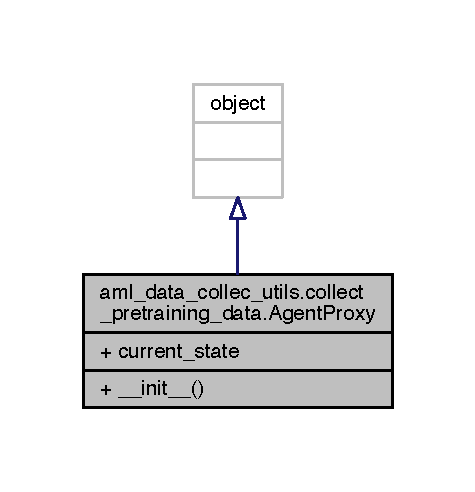
\includegraphics[width=224pt]{classaml__data__collec__utils_1_1collect__pretraining__data_1_1_agent_proxy__inherit__graph}
\end{center}
\end{figure}


Collaboration diagram for aml\-\_\-data\-\_\-collec\-\_\-utils.\-collect\-\_\-pretraining\-\_\-data.\-Agent\-Proxy\-:
\nopagebreak
\begin{figure}[H]
\begin{center}
\leavevmode
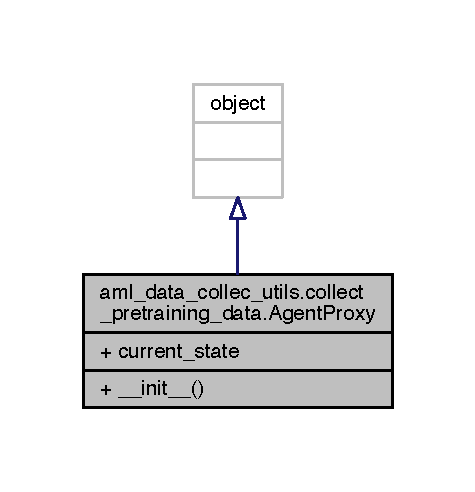
\includegraphics[width=224pt]{classaml__data__collec__utils_1_1collect__pretraining__data_1_1_agent_proxy__coll__graph}
\end{center}
\end{figure}
\subsection*{Public Member Functions}
\begin{DoxyCompactItemize}
\item 
\hypertarget{classaml__data__collec__utils_1_1collect__pretraining__data_1_1_agent_proxy_a0ba09dbbb1e176464aa07485f77cf9f9}{def {\bfseries \-\_\-\-\_\-init\-\_\-\-\_\-}}\label{classaml__data__collec__utils_1_1collect__pretraining__data_1_1_agent_proxy_a0ba09dbbb1e176464aa07485f77cf9f9}

\end{DoxyCompactItemize}
\subsection*{Public Attributes}
\begin{DoxyCompactItemize}
\item 
\hypertarget{classaml__data__collec__utils_1_1collect__pretraining__data_1_1_agent_proxy_aeb2225b6b78553e00dfa022cd7bafd49}{{\bfseries current\-\_\-state}}\label{classaml__data__collec__utils_1_1collect__pretraining__data_1_1_agent_proxy_aeb2225b6b78553e00dfa022cd7bafd49}

\end{DoxyCompactItemize}


The documentation for this class was generated from the following file\-:\begin{DoxyCompactItemize}
\item 
aml\-\_\-data\-\_\-collec\-\_\-utils/src/aml\-\_\-data\-\_\-collec\-\_\-utils/collect\-\_\-pretraining\-\_\-data.\-py\end{DoxyCompactItemize}

\hypertarget{classaml__io_1_1log__utils_1_1aml__logging}{}\section{aml\+\_\+io.\+log\+\_\+utils.\+aml\+\_\+logging Class Reference}
\label{classaml__io_1_1log__utils_1_1aml__logging}\index{aml\+\_\+io.\+log\+\_\+utils.\+aml\+\_\+logging@{aml\+\_\+io.\+log\+\_\+utils.\+aml\+\_\+logging}}


Inheritance diagram for aml\+\_\+io.\+log\+\_\+utils.\+aml\+\_\+logging\+:
\nopagebreak
\begin{figure}[H]
\begin{center}
\leavevmode
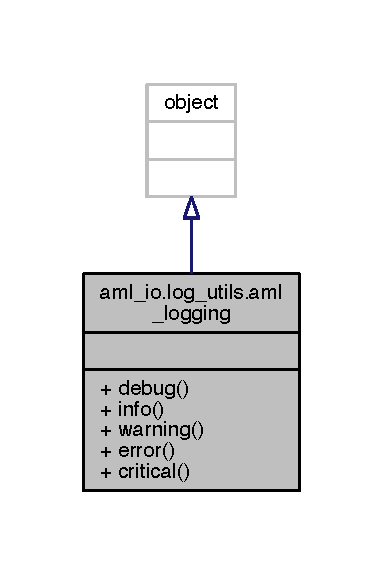
\includegraphics[width=184pt]{classaml__io_1_1log__utils_1_1aml__logging__inherit__graph}
\end{center}
\end{figure}


Collaboration diagram for aml\+\_\+io.\+log\+\_\+utils.\+aml\+\_\+logging\+:
\nopagebreak
\begin{figure}[H]
\begin{center}
\leavevmode
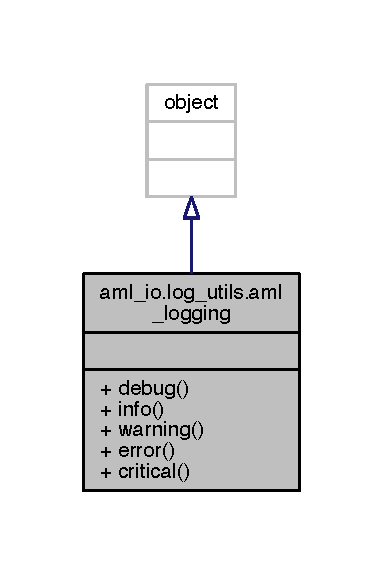
\includegraphics[width=184pt]{classaml__io_1_1log__utils_1_1aml__logging__coll__graph}
\end{center}
\end{figure}
\subsection*{Public Member Functions}
\begin{DoxyCompactItemize}
\item 
\hypertarget{classaml__io_1_1log__utils_1_1aml__logging_a841598eda325337f33a5f833384597ed}{}\label{classaml__io_1_1log__utils_1_1aml__logging_a841598eda325337f33a5f833384597ed} 
def {\bfseries debug} (cls, msg)
\item 
\hypertarget{classaml__io_1_1log__utils_1_1aml__logging_a35f613505f381c5c150211a19248897f}{}\label{classaml__io_1_1log__utils_1_1aml__logging_a35f613505f381c5c150211a19248897f} 
def {\bfseries info} (cls, msg)
\item 
\hypertarget{classaml__io_1_1log__utils_1_1aml__logging_a0d9a6a65dbc9e3d266a6bf8791ddd1c3}{}\label{classaml__io_1_1log__utils_1_1aml__logging_a0d9a6a65dbc9e3d266a6bf8791ddd1c3} 
def {\bfseries warning} (cls, msg)
\item 
\hypertarget{classaml__io_1_1log__utils_1_1aml__logging_ab88893a3ae1aa41bdf4c401af9f8a3b4}{}\label{classaml__io_1_1log__utils_1_1aml__logging_ab88893a3ae1aa41bdf4c401af9f8a3b4} 
def {\bfseries error} (cls, msg)
\item 
\hypertarget{classaml__io_1_1log__utils_1_1aml__logging_a2c3d6b9d2cc80d959da7f12cdf02a633}{}\label{classaml__io_1_1log__utils_1_1aml__logging_a2c3d6b9d2cc80d959da7f12cdf02a633} 
def {\bfseries critical} (cls, msg)
\end{DoxyCompactItemize}


The documentation for this class was generated from the following file\+:\begin{DoxyCompactItemize}
\item 
aml\+\_\+io/src/aml\+\_\+io/log\+\_\+utils.\+py\end{DoxyCompactItemize}

\hypertarget{classsrc_1_1aml__dl_1_1utilities_1_1tf__batch__creator_1_1_batch_creator}{\section{src.\-aml\-\_\-dl.\-utilities.\-tf\-\_\-batch\-\_\-creator.\-Batch\-Creator Class Reference}
\label{classsrc_1_1aml__dl_1_1utilities_1_1tf__batch__creator_1_1_batch_creator}\index{src.\-aml\-\_\-dl.\-utilities.\-tf\-\_\-batch\-\_\-creator.\-Batch\-Creator@{src.\-aml\-\_\-dl.\-utilities.\-tf\-\_\-batch\-\_\-creator.\-Batch\-Creator}}
}


Inheritance diagram for src.\-aml\-\_\-dl.\-utilities.\-tf\-\_\-batch\-\_\-creator.\-Batch\-Creator\-:
\nopagebreak
\begin{figure}[H]
\begin{center}
\leavevmode
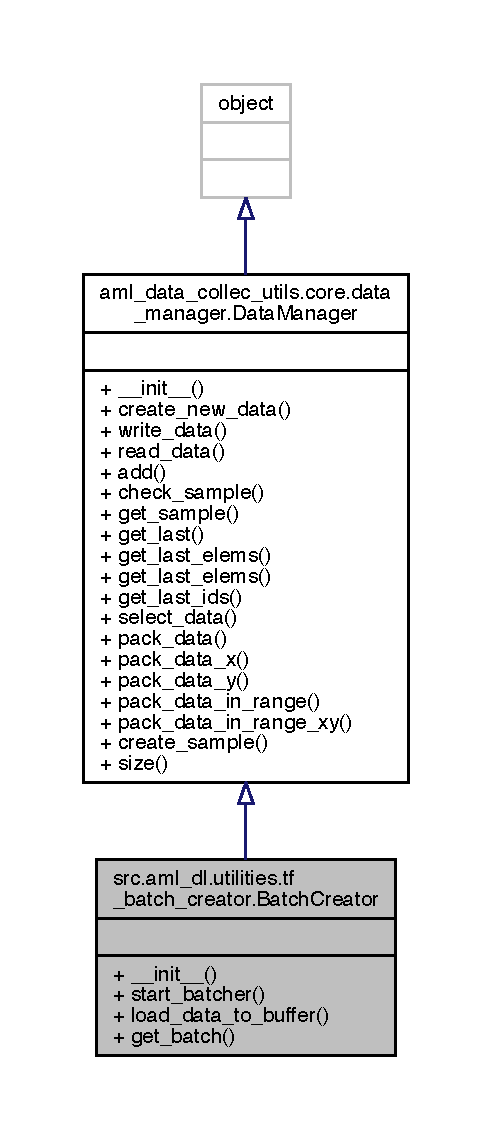
\includegraphics[height=550pt]{classsrc_1_1aml__dl_1_1utilities_1_1tf__batch__creator_1_1_batch_creator__inherit__graph}
\end{center}
\end{figure}


Collaboration diagram for src.\-aml\-\_\-dl.\-utilities.\-tf\-\_\-batch\-\_\-creator.\-Batch\-Creator\-:
\nopagebreak
\begin{figure}[H]
\begin{center}
\leavevmode
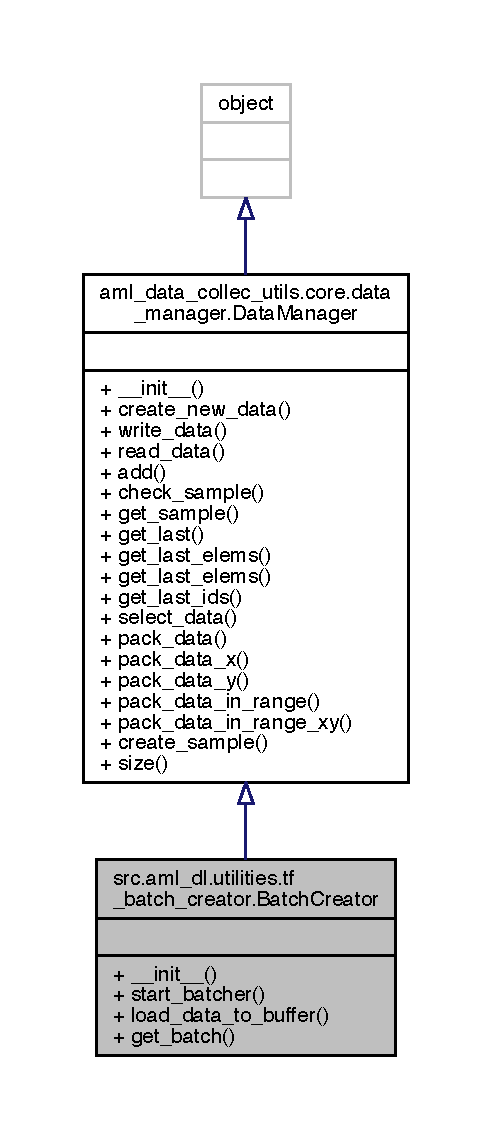
\includegraphics[height=550pt]{classsrc_1_1aml__dl_1_1utilities_1_1tf__batch__creator_1_1_batch_creator__coll__graph}
\end{center}
\end{figure}
\subsection*{Public Member Functions}
\begin{DoxyCompactItemize}
\item 
\hypertarget{classsrc_1_1aml__dl_1_1utilities_1_1tf__batch__creator_1_1_batch_creator_ab50c3143c3affca454228d60a2f5bb96}{def {\bfseries \-\_\-\-\_\-init\-\_\-\-\_\-}}\label{classsrc_1_1aml__dl_1_1utilities_1_1tf__batch__creator_1_1_batch_creator_ab50c3143c3affca454228d60a2f5bb96}

\item 
\hypertarget{classsrc_1_1aml__dl_1_1utilities_1_1tf__batch__creator_1_1_batch_creator_a19457cb3db9b6ac13b93755bbe7c12de}{def {\bfseries start\-\_\-batcher}}\label{classsrc_1_1aml__dl_1_1utilities_1_1tf__batch__creator_1_1_batch_creator_a19457cb3db9b6ac13b93755bbe7c12de}

\item 
\hypertarget{classsrc_1_1aml__dl_1_1utilities_1_1tf__batch__creator_1_1_batch_creator_a34ae5372026672a949991b4be886b8b1}{def {\bfseries load\-\_\-data\-\_\-to\-\_\-buffer}}\label{classsrc_1_1aml__dl_1_1utilities_1_1tf__batch__creator_1_1_batch_creator_a34ae5372026672a949991b4be886b8b1}

\item 
\hypertarget{classsrc_1_1aml__dl_1_1utilities_1_1tf__batch__creator_1_1_batch_creator_a49ef8b29356437b4b6be4948d1f51366}{def {\bfseries get\-\_\-batch}}\label{classsrc_1_1aml__dl_1_1utilities_1_1tf__batch__creator_1_1_batch_creator_a49ef8b29356437b4b6be4948d1f51366}

\end{DoxyCompactItemize}


The documentation for this class was generated from the following file\-:\begin{DoxyCompactItemize}
\item 
aml\-\_\-dl/src/aml\-\_\-dl/utilities/tf\-\_\-batch\-\_\-creator.\-py\end{DoxyCompactItemize}

\hypertarget{classaml__robot_1_1baxter__kinematics_1_1baxter__kinematics}{\section{aml\-\_\-robot.\-baxter\-\_\-kinematics.\-baxter\-\_\-kinematics Class Reference}
\label{classaml__robot_1_1baxter__kinematics_1_1baxter__kinematics}\index{aml\-\_\-robot.\-baxter\-\_\-kinematics.\-baxter\-\_\-kinematics@{aml\-\_\-robot.\-baxter\-\_\-kinematics.\-baxter\-\_\-kinematics}}
}


Inheritance diagram for aml\-\_\-robot.\-baxter\-\_\-kinematics.\-baxter\-\_\-kinematics\-:\nopagebreak
\begin{figure}[H]
\begin{center}
\leavevmode
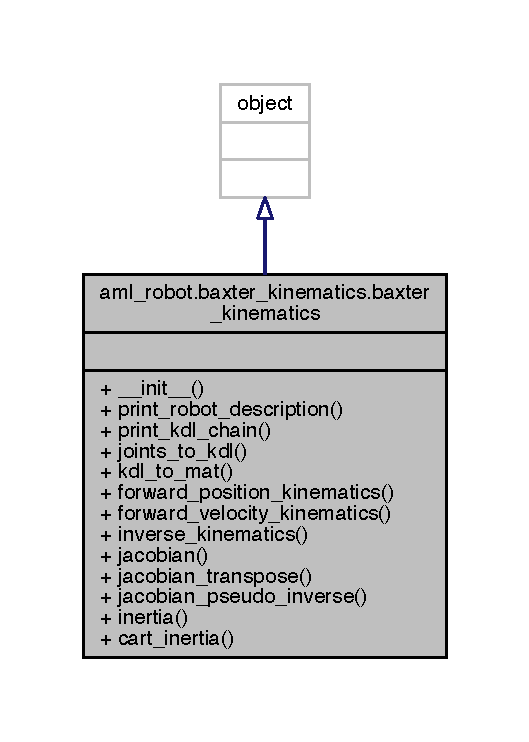
\includegraphics[width=252pt]{classaml__robot_1_1baxter__kinematics_1_1baxter__kinematics__inherit__graph}
\end{center}
\end{figure}


Collaboration diagram for aml\-\_\-robot.\-baxter\-\_\-kinematics.\-baxter\-\_\-kinematics\-:\nopagebreak
\begin{figure}[H]
\begin{center}
\leavevmode
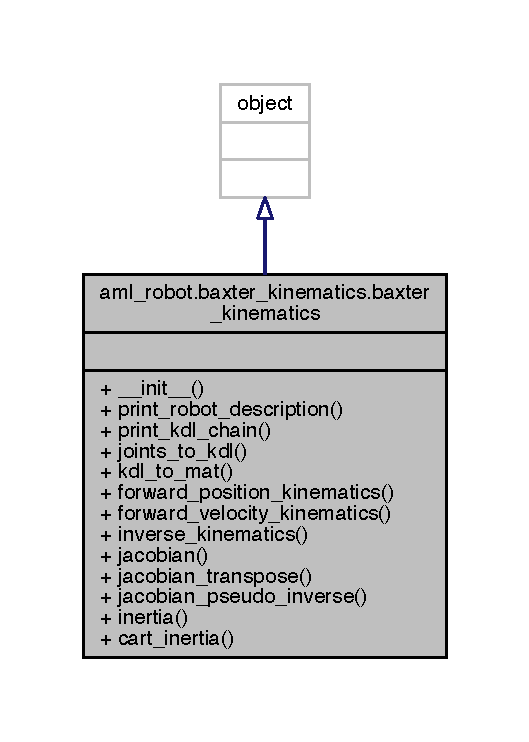
\includegraphics[width=252pt]{classaml__robot_1_1baxter__kinematics_1_1baxter__kinematics__coll__graph}
\end{center}
\end{figure}
\subsection*{Public Member Functions}
\begin{DoxyCompactItemize}
\item 
\hypertarget{classaml__robot_1_1baxter__kinematics_1_1baxter__kinematics_a6a642546348903ad83647e46b3997319}{def {\bfseries \-\_\-\-\_\-init\-\_\-\-\_\-}}\label{classaml__robot_1_1baxter__kinematics_1_1baxter__kinematics_a6a642546348903ad83647e46b3997319}

\item 
\hypertarget{classaml__robot_1_1baxter__kinematics_1_1baxter__kinematics_a5f20f5ed9f8e063544fe0f9269824d77}{def {\bfseries print\-\_\-robot\-\_\-description}}\label{classaml__robot_1_1baxter__kinematics_1_1baxter__kinematics_a5f20f5ed9f8e063544fe0f9269824d77}

\item 
\hypertarget{classaml__robot_1_1baxter__kinematics_1_1baxter__kinematics_a6505980cb91459683b46b4eb0ed5048f}{def {\bfseries print\-\_\-kdl\-\_\-chain}}\label{classaml__robot_1_1baxter__kinematics_1_1baxter__kinematics_a6505980cb91459683b46b4eb0ed5048f}

\item 
\hypertarget{classaml__robot_1_1baxter__kinematics_1_1baxter__kinematics_a5b33fe6f350f58a6b1eab83aa072d847}{def {\bfseries joints\-\_\-to\-\_\-kdl}}\label{classaml__robot_1_1baxter__kinematics_1_1baxter__kinematics_a5b33fe6f350f58a6b1eab83aa072d847}

\item 
\hypertarget{classaml__robot_1_1baxter__kinematics_1_1baxter__kinematics_a4b961c3b58138f41aa1b0f4f34da7e83}{def {\bfseries kdl\-\_\-to\-\_\-mat}}\label{classaml__robot_1_1baxter__kinematics_1_1baxter__kinematics_a4b961c3b58138f41aa1b0f4f34da7e83}

\item 
\hypertarget{classaml__robot_1_1baxter__kinematics_1_1baxter__kinematics_a4c3c9043ae935f5ae5c4bb5806532071}{def {\bfseries forward\-\_\-position\-\_\-kinematics}}\label{classaml__robot_1_1baxter__kinematics_1_1baxter__kinematics_a4c3c9043ae935f5ae5c4bb5806532071}

\item 
\hypertarget{classaml__robot_1_1baxter__kinematics_1_1baxter__kinematics_aca2eef593f0f9e6095c13153401eb948}{def {\bfseries forward\-\_\-velocity\-\_\-kinematics}}\label{classaml__robot_1_1baxter__kinematics_1_1baxter__kinematics_aca2eef593f0f9e6095c13153401eb948}

\item 
\hypertarget{classaml__robot_1_1baxter__kinematics_1_1baxter__kinematics_a5eaca30766683990b213182527cb3813}{def {\bfseries inverse\-\_\-kinematics}}\label{classaml__robot_1_1baxter__kinematics_1_1baxter__kinematics_a5eaca30766683990b213182527cb3813}

\item 
\hypertarget{classaml__robot_1_1baxter__kinematics_1_1baxter__kinematics_a307997661ec9ef26ae4a74bda67a3352}{def {\bfseries jacobian}}\label{classaml__robot_1_1baxter__kinematics_1_1baxter__kinematics_a307997661ec9ef26ae4a74bda67a3352}

\item 
\hypertarget{classaml__robot_1_1baxter__kinematics_1_1baxter__kinematics_a421d5a7383a8b88e7b03efc469f30098}{def {\bfseries jacobian\-\_\-transpose}}\label{classaml__robot_1_1baxter__kinematics_1_1baxter__kinematics_a421d5a7383a8b88e7b03efc469f30098}

\item 
\hypertarget{classaml__robot_1_1baxter__kinematics_1_1baxter__kinematics_ad70f0257064b8a85ee6537e2187822d8}{def {\bfseries jacobian\-\_\-pseudo\-\_\-inverse}}\label{classaml__robot_1_1baxter__kinematics_1_1baxter__kinematics_ad70f0257064b8a85ee6537e2187822d8}

\item 
\hypertarget{classaml__robot_1_1baxter__kinematics_1_1baxter__kinematics_a7fd0653ad6b2012a933822f98901ccce}{def {\bfseries inertia}}\label{classaml__robot_1_1baxter__kinematics_1_1baxter__kinematics_a7fd0653ad6b2012a933822f98901ccce}

\item 
\hypertarget{classaml__robot_1_1baxter__kinematics_1_1baxter__kinematics_af243bf47f45355fb5e71a23ed8b21d28}{def {\bfseries cart\-\_\-inertia}}\label{classaml__robot_1_1baxter__kinematics_1_1baxter__kinematics_af243bf47f45355fb5e71a23ed8b21d28}

\end{DoxyCompactItemize}


\subsection{Detailed Description}
\begin{DoxyVerb}Baxter Kinematics with PyKDL
\end{DoxyVerb}
 

The documentation for this class was generated from the following file\-:\begin{DoxyCompactItemize}
\item 
aml\-\_\-robot/src/aml\-\_\-robot/baxter\-\_\-kinematics.\-py\end{DoxyCompactItemize}

\hypertarget{classaml__robot_1_1baxter__robot_1_1_baxter_arm}{}\section{aml\+\_\+robot.\+baxter\+\_\+robot.\+Baxter\+Arm Class Reference}
\label{classaml__robot_1_1baxter__robot_1_1_baxter_arm}\index{aml\+\_\+robot.\+baxter\+\_\+robot.\+Baxter\+Arm@{aml\+\_\+robot.\+baxter\+\_\+robot.\+Baxter\+Arm}}


Inheritance diagram for aml\+\_\+robot.\+baxter\+\_\+robot.\+Baxter\+Arm\+:
\nopagebreak
\begin{figure}[H]
\begin{center}
\leavevmode
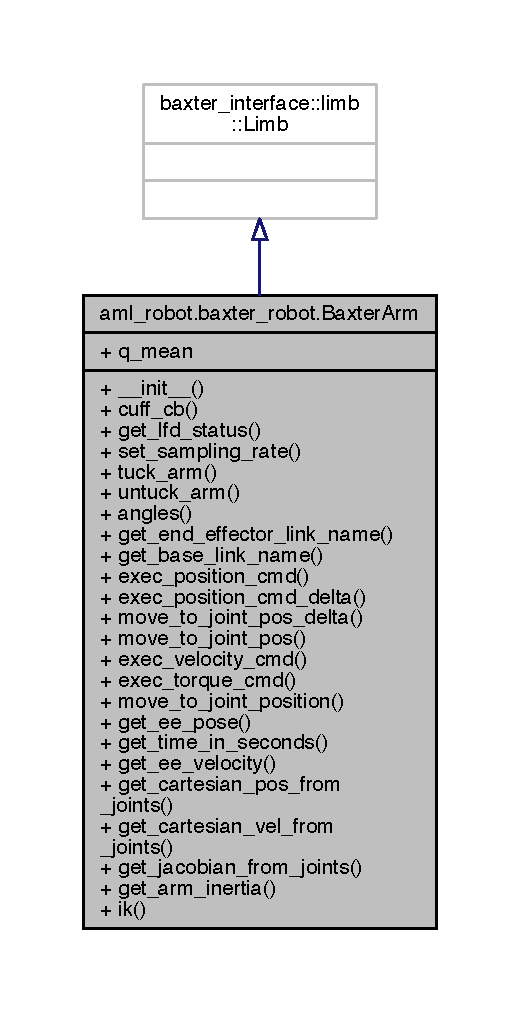
\includegraphics[width=249pt]{classaml__robot_1_1baxter__robot_1_1_baxter_arm__inherit__graph}
\end{center}
\end{figure}


Collaboration diagram for aml\+\_\+robot.\+baxter\+\_\+robot.\+Baxter\+Arm\+:
\nopagebreak
\begin{figure}[H]
\begin{center}
\leavevmode
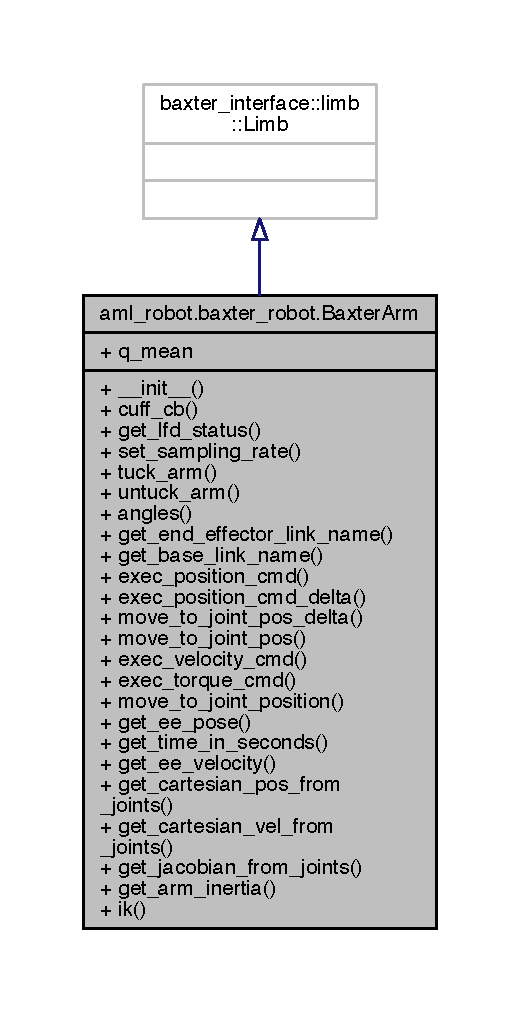
\includegraphics[width=249pt]{classaml__robot_1_1baxter__robot_1_1_baxter_arm__coll__graph}
\end{center}
\end{figure}
\subsection*{Public Member Functions}
\begin{DoxyCompactItemize}
\item 
\hypertarget{classaml__robot_1_1baxter__robot_1_1_baxter_arm_a72a5c161c29bd536c6a8727d3138643a}{}\label{classaml__robot_1_1baxter__robot_1_1_baxter_arm_a72a5c161c29bd536c6a8727d3138643a} 
def {\bfseries \+\_\+\+\_\+init\+\_\+\+\_\+} (self, limb, on\+\_\+state\+\_\+callback=None)
\item 
\hypertarget{classaml__robot_1_1baxter__robot_1_1_baxter_arm_ab8c5985c2c013d2da84e7415f2480f35}{}\label{classaml__robot_1_1baxter__robot_1_1_baxter_arm_ab8c5985c2c013d2da84e7415f2480f35} 
def {\bfseries cuff\+\_\+cb} (self, value)
\item 
\hypertarget{classaml__robot_1_1baxter__robot_1_1_baxter_arm_a08034a334645d8504b391a313add1cc7}{}\label{classaml__robot_1_1baxter__robot_1_1_baxter_arm_a08034a334645d8504b391a313add1cc7} 
def {\bfseries get\+\_\+lfd\+\_\+status} (self)
\item 
\hypertarget{classaml__robot_1_1baxter__robot_1_1_baxter_arm_a1f1b2c10d8e309c0cce60a971f5355b4}{}\label{classaml__robot_1_1baxter__robot_1_1_baxter_arm_a1f1b2c10d8e309c0cce60a971f5355b4} 
def {\bfseries set\+\_\+sampling\+\_\+rate} (self, sampling\+\_\+rate=100)
\item 
\hypertarget{classaml__robot_1_1baxter__robot_1_1_baxter_arm_add8768944b81542e122c676f2b38c075}{}\label{classaml__robot_1_1baxter__robot_1_1_baxter_arm_add8768944b81542e122c676f2b38c075} 
def {\bfseries tuck\+\_\+arm} (self)
\item 
\hypertarget{classaml__robot_1_1baxter__robot_1_1_baxter_arm_af3664aaae25213bf3930c821cbf68432}{}\label{classaml__robot_1_1baxter__robot_1_1_baxter_arm_af3664aaae25213bf3930c821cbf68432} 
def {\bfseries untuck\+\_\+arm} (self)
\item 
\hypertarget{classaml__robot_1_1baxter__robot_1_1_baxter_arm_a0434abfd5899e880a6856444ccc9ecae}{}\label{classaml__robot_1_1baxter__robot_1_1_baxter_arm_a0434abfd5899e880a6856444ccc9ecae} 
def {\bfseries angles} (self)
\item 
\hypertarget{classaml__robot_1_1baxter__robot_1_1_baxter_arm_a40dc93e2269ea57aec71457431984bc0}{}\label{classaml__robot_1_1baxter__robot_1_1_baxter_arm_a40dc93e2269ea57aec71457431984bc0} 
def {\bfseries get\+\_\+end\+\_\+effector\+\_\+link\+\_\+name} (self)
\item 
\hypertarget{classaml__robot_1_1baxter__robot_1_1_baxter_arm_a3d7c1dd8493d6ed1255e856db43e4d9c}{}\label{classaml__robot_1_1baxter__robot_1_1_baxter_arm_a3d7c1dd8493d6ed1255e856db43e4d9c} 
def {\bfseries get\+\_\+base\+\_\+link\+\_\+name} (self)
\item 
\hypertarget{classaml__robot_1_1baxter__robot_1_1_baxter_arm_aa8fb038222939675c5038f546d0e2627}{}\label{classaml__robot_1_1baxter__robot_1_1_baxter_arm_aa8fb038222939675c5038f546d0e2627} 
def {\bfseries exec\+\_\+position\+\_\+cmd} (self, cmd)
\item 
\hypertarget{classaml__robot_1_1baxter__robot_1_1_baxter_arm_a7231f60bcd22ea25ee84d5c3269e82ae}{}\label{classaml__robot_1_1baxter__robot_1_1_baxter_arm_a7231f60bcd22ea25ee84d5c3269e82ae} 
def {\bfseries exec\+\_\+position\+\_\+cmd\+\_\+delta} (self, cmd)
\item 
\hypertarget{classaml__robot_1_1baxter__robot_1_1_baxter_arm_ad4c0f6a22d0cb23f411d50e8f661bcbb}{}\label{classaml__robot_1_1baxter__robot_1_1_baxter_arm_ad4c0f6a22d0cb23f411d50e8f661bcbb} 
def {\bfseries move\+\_\+to\+\_\+joint\+\_\+pos\+\_\+delta} (self, cmd)
\item 
\hypertarget{classaml__robot_1_1baxter__robot_1_1_baxter_arm_a93f87a8500f9e0bfce6be75e41e3ac17}{}\label{classaml__robot_1_1baxter__robot_1_1_baxter_arm_a93f87a8500f9e0bfce6be75e41e3ac17} 
def {\bfseries move\+\_\+to\+\_\+joint\+\_\+pos} (self, cmd)
\item 
\hypertarget{classaml__robot_1_1baxter__robot_1_1_baxter_arm_a3b5cb3d6c651c72bfe9ffd80c867f8f7}{}\label{classaml__robot_1_1baxter__robot_1_1_baxter_arm_a3b5cb3d6c651c72bfe9ffd80c867f8f7} 
def {\bfseries exec\+\_\+velocity\+\_\+cmd} (self, cmd)
\item 
\hypertarget{classaml__robot_1_1baxter__robot_1_1_baxter_arm_aed8c9accc1f637677e4d64583b63d107}{}\label{classaml__robot_1_1baxter__robot_1_1_baxter_arm_aed8c9accc1f637677e4d64583b63d107} 
def {\bfseries exec\+\_\+torque\+\_\+cmd} (self, cmd)
\item 
\hypertarget{classaml__robot_1_1baxter__robot_1_1_baxter_arm_afddcdfa0cafe258cf7f432e7878bc687}{}\label{classaml__robot_1_1baxter__robot_1_1_baxter_arm_afddcdfa0cafe258cf7f432e7878bc687} 
def {\bfseries move\+\_\+to\+\_\+joint\+\_\+position} (self, joint\+\_\+angles)
\item 
\hypertarget{classaml__robot_1_1baxter__robot_1_1_baxter_arm_ac353cdab96098923a40efd30f17f4e7a}{}\label{classaml__robot_1_1baxter__robot_1_1_baxter_arm_ac353cdab96098923a40efd30f17f4e7a} 
def {\bfseries get\+\_\+ee\+\_\+pose} (self)
\item 
\hypertarget{classaml__robot_1_1baxter__robot_1_1_baxter_arm_a9dcc207d5f7703f7f9f69bb54c1ee7b3}{}\label{classaml__robot_1_1baxter__robot_1_1_baxter_arm_a9dcc207d5f7703f7f9f69bb54c1ee7b3} 
def {\bfseries get\+\_\+time\+\_\+in\+\_\+seconds} (self)
\item 
\hypertarget{classaml__robot_1_1baxter__robot_1_1_baxter_arm_a411092f179a7420d38625063c27b237e}{}\label{classaml__robot_1_1baxter__robot_1_1_baxter_arm_a411092f179a7420d38625063c27b237e} 
def {\bfseries get\+\_\+ee\+\_\+velocity} (self, real\+\_\+robot=True)
\item 
\hypertarget{classaml__robot_1_1baxter__robot_1_1_baxter_arm_a9ce9c74c445092b5f9bd26793366c8de}{}\label{classaml__robot_1_1baxter__robot_1_1_baxter_arm_a9ce9c74c445092b5f9bd26793366c8de} 
def {\bfseries get\+\_\+cartesian\+\_\+pos\+\_\+from\+\_\+joints} (self, joint\+\_\+angles=None)
\item 
\hypertarget{classaml__robot_1_1baxter__robot_1_1_baxter_arm_a5d42a91ca13fc1776997909afb999d8f}{}\label{classaml__robot_1_1baxter__robot_1_1_baxter_arm_a5d42a91ca13fc1776997909afb999d8f} 
def {\bfseries get\+\_\+cartesian\+\_\+vel\+\_\+from\+\_\+joints} (self, joint\+\_\+angles=None)
\item 
\hypertarget{classaml__robot_1_1baxter__robot_1_1_baxter_arm_a05c9ee1fe630edbcdc34249bb0c613b3}{}\label{classaml__robot_1_1baxter__robot_1_1_baxter_arm_a05c9ee1fe630edbcdc34249bb0c613b3} 
def {\bfseries get\+\_\+jacobian\+\_\+from\+\_\+joints} (self, joint\+\_\+angles=None)
\item 
\hypertarget{classaml__robot_1_1baxter__robot_1_1_baxter_arm_ae3980ca9408490d07b4460e6d7fc2eb2}{}\label{classaml__robot_1_1baxter__robot_1_1_baxter_arm_ae3980ca9408490d07b4460e6d7fc2eb2} 
def {\bfseries get\+\_\+arm\+\_\+inertia} (self, joint\+\_\+angles=None)
\item 
\hypertarget{classaml__robot_1_1baxter__robot_1_1_baxter_arm_a5ce4a9920b76e223e375755faaef7cf5}{}\label{classaml__robot_1_1baxter__robot_1_1_baxter_arm_a5ce4a9920b76e223e375755faaef7cf5} 
def {\bfseries ik} (self, pos, ori=None)
\end{DoxyCompactItemize}
\subsection*{Public Attributes}
\begin{DoxyCompactItemize}
\item 
\hypertarget{classaml__robot_1_1baxter__robot_1_1_baxter_arm_adf4365cfefdb2632a538a3f225023aa7}{}\label{classaml__robot_1_1baxter__robot_1_1_baxter_arm_adf4365cfefdb2632a538a3f225023aa7} 
{\bfseries q\+\_\+mean}
\end{DoxyCompactItemize}


The documentation for this class was generated from the following file\+:\begin{DoxyCompactItemize}
\item 
aml\+\_\+robot/src/aml\+\_\+robot/baxter\+\_\+robot.\+py\end{DoxyCompactItemize}

\hypertarget{classaml__robot_1_1baxter__robot_1_1_baxter_button_status}{}\section{aml\+\_\+robot.\+baxter\+\_\+robot.\+Baxter\+Button\+Status Class Reference}
\label{classaml__robot_1_1baxter__robot_1_1_baxter_button_status}\index{aml\+\_\+robot.\+baxter\+\_\+robot.\+Baxter\+Button\+Status@{aml\+\_\+robot.\+baxter\+\_\+robot.\+Baxter\+Button\+Status}}


Collaboration diagram for aml\+\_\+robot.\+baxter\+\_\+robot.\+Baxter\+Button\+Status\+:
\nopagebreak
\begin{figure}[H]
\begin{center}
\leavevmode
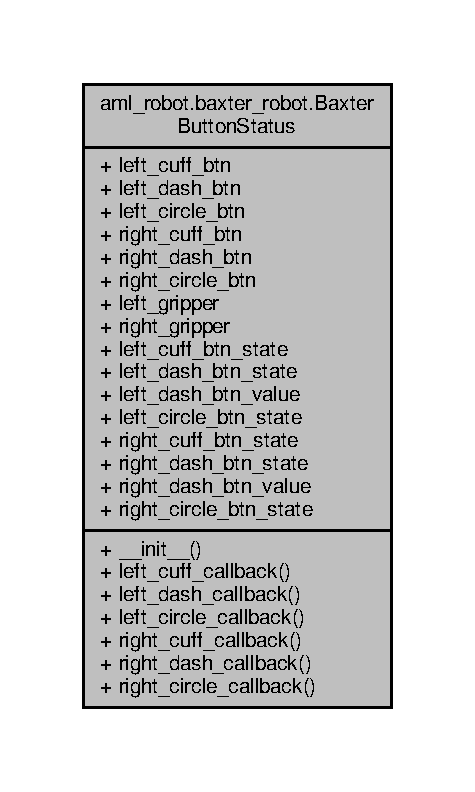
\includegraphics[width=231pt]{classaml__robot_1_1baxter__robot_1_1_baxter_button_status__coll__graph}
\end{center}
\end{figure}
\subsection*{Public Member Functions}
\begin{DoxyCompactItemize}
\item 
\hypertarget{classaml__robot_1_1baxter__robot_1_1_baxter_button_status_a867cbab0efc9f033f193484b7a6ee7d9}{}\label{classaml__robot_1_1baxter__robot_1_1_baxter_button_status_a867cbab0efc9f033f193484b7a6ee7d9} 
def {\bfseries \+\_\+\+\_\+init\+\_\+\+\_\+} (self)
\item 
\hypertarget{classaml__robot_1_1baxter__robot_1_1_baxter_button_status_a0be7e8628a069cee960ba4f84a1fba42}{}\label{classaml__robot_1_1baxter__robot_1_1_baxter_button_status_a0be7e8628a069cee960ba4f84a1fba42} 
def {\bfseries left\+\_\+cuff\+\_\+callback} (self, value)
\item 
\hypertarget{classaml__robot_1_1baxter__robot_1_1_baxter_button_status_a0c7539db9445b453a0eac9e24d402b89}{}\label{classaml__robot_1_1baxter__robot_1_1_baxter_button_status_a0c7539db9445b453a0eac9e24d402b89} 
def {\bfseries left\+\_\+dash\+\_\+callback} (self, value)
\item 
\hypertarget{classaml__robot_1_1baxter__robot_1_1_baxter_button_status_a2a5e12090c441e098b287596bac9b2e9}{}\label{classaml__robot_1_1baxter__robot_1_1_baxter_button_status_a2a5e12090c441e098b287596bac9b2e9} 
def {\bfseries left\+\_\+circle\+\_\+callback} (self, value)
\item 
\hypertarget{classaml__robot_1_1baxter__robot_1_1_baxter_button_status_aea7f6e2c3cb75cc764898bacdf24adad}{}\label{classaml__robot_1_1baxter__robot_1_1_baxter_button_status_aea7f6e2c3cb75cc764898bacdf24adad} 
def {\bfseries right\+\_\+cuff\+\_\+callback} (self, value)
\item 
\hypertarget{classaml__robot_1_1baxter__robot_1_1_baxter_button_status_a9ebd13514e6d978c3a022b99f56d0d2d}{}\label{classaml__robot_1_1baxter__robot_1_1_baxter_button_status_a9ebd13514e6d978c3a022b99f56d0d2d} 
def {\bfseries right\+\_\+dash\+\_\+callback} (self, value)
\item 
\hypertarget{classaml__robot_1_1baxter__robot_1_1_baxter_button_status_a80e8aebd2bf7ceb32d63bade6e078eff}{}\label{classaml__robot_1_1baxter__robot_1_1_baxter_button_status_a80e8aebd2bf7ceb32d63bade6e078eff} 
def {\bfseries right\+\_\+circle\+\_\+callback} (self, value)
\end{DoxyCompactItemize}
\subsection*{Public Attributes}
\begin{DoxyCompactItemize}
\item 
\hypertarget{classaml__robot_1_1baxter__robot_1_1_baxter_button_status_a04619f9d86af362ba45b652a30f75186}{}\label{classaml__robot_1_1baxter__robot_1_1_baxter_button_status_a04619f9d86af362ba45b652a30f75186} 
{\bfseries left\+\_\+cuff\+\_\+btn}
\item 
\hypertarget{classaml__robot_1_1baxter__robot_1_1_baxter_button_status_a8bf46c388908af610775a7853f12db6b}{}\label{classaml__robot_1_1baxter__robot_1_1_baxter_button_status_a8bf46c388908af610775a7853f12db6b} 
{\bfseries left\+\_\+dash\+\_\+btn}
\item 
\hypertarget{classaml__robot_1_1baxter__robot_1_1_baxter_button_status_aafc55b8a39cd12b8b916c1f9e4e101cb}{}\label{classaml__robot_1_1baxter__robot_1_1_baxter_button_status_aafc55b8a39cd12b8b916c1f9e4e101cb} 
{\bfseries left\+\_\+circle\+\_\+btn}
\item 
\hypertarget{classaml__robot_1_1baxter__robot_1_1_baxter_button_status_a96d1d159449f8937e2c8605ffb359e26}{}\label{classaml__robot_1_1baxter__robot_1_1_baxter_button_status_a96d1d159449f8937e2c8605ffb359e26} 
{\bfseries right\+\_\+cuff\+\_\+btn}
\item 
\hypertarget{classaml__robot_1_1baxter__robot_1_1_baxter_button_status_a20e886d155229257692984a1fc790216}{}\label{classaml__robot_1_1baxter__robot_1_1_baxter_button_status_a20e886d155229257692984a1fc790216} 
{\bfseries right\+\_\+dash\+\_\+btn}
\item 
\hypertarget{classaml__robot_1_1baxter__robot_1_1_baxter_button_status_af554ad16b5a28ab857cdc6c1d0e92ad8}{}\label{classaml__robot_1_1baxter__robot_1_1_baxter_button_status_af554ad16b5a28ab857cdc6c1d0e92ad8} 
{\bfseries right\+\_\+circle\+\_\+btn}
\item 
\hypertarget{classaml__robot_1_1baxter__robot_1_1_baxter_button_status_a1c2a8b264d928929fa9cad5d97bdc817}{}\label{classaml__robot_1_1baxter__robot_1_1_baxter_button_status_a1c2a8b264d928929fa9cad5d97bdc817} 
{\bfseries left\+\_\+gripper}
\item 
\hypertarget{classaml__robot_1_1baxter__robot_1_1_baxter_button_status_a1dd2e91ddd93d9c40dc8e7f83926d908}{}\label{classaml__robot_1_1baxter__robot_1_1_baxter_button_status_a1dd2e91ddd93d9c40dc8e7f83926d908} 
{\bfseries right\+\_\+gripper}
\item 
\hypertarget{classaml__robot_1_1baxter__robot_1_1_baxter_button_status_a3d147c0e2ab38474d2cb2d2cb358e9c6}{}\label{classaml__robot_1_1baxter__robot_1_1_baxter_button_status_a3d147c0e2ab38474d2cb2d2cb358e9c6} 
{\bfseries left\+\_\+cuff\+\_\+btn\+\_\+state}
\item 
\hypertarget{classaml__robot_1_1baxter__robot_1_1_baxter_button_status_a9858defbdfd1953111bc032a679dfbf6}{}\label{classaml__robot_1_1baxter__robot_1_1_baxter_button_status_a9858defbdfd1953111bc032a679dfbf6} 
{\bfseries left\+\_\+dash\+\_\+btn\+\_\+state}
\item 
\hypertarget{classaml__robot_1_1baxter__robot_1_1_baxter_button_status_ac4505635cb0c3096d50145a00aa996e1}{}\label{classaml__robot_1_1baxter__robot_1_1_baxter_button_status_ac4505635cb0c3096d50145a00aa996e1} 
{\bfseries left\+\_\+dash\+\_\+btn\+\_\+value}
\item 
\hypertarget{classaml__robot_1_1baxter__robot_1_1_baxter_button_status_a2cf8425649007e50335a7eab640138bd}{}\label{classaml__robot_1_1baxter__robot_1_1_baxter_button_status_a2cf8425649007e50335a7eab640138bd} 
{\bfseries left\+\_\+circle\+\_\+btn\+\_\+state}
\item 
\hypertarget{classaml__robot_1_1baxter__robot_1_1_baxter_button_status_a0b2de8e8474d9e9217024692b425a0b4}{}\label{classaml__robot_1_1baxter__robot_1_1_baxter_button_status_a0b2de8e8474d9e9217024692b425a0b4} 
{\bfseries right\+\_\+cuff\+\_\+btn\+\_\+state}
\item 
\hypertarget{classaml__robot_1_1baxter__robot_1_1_baxter_button_status_a99abdcffd19c44a10cb1f4a875adbb2d}{}\label{classaml__robot_1_1baxter__robot_1_1_baxter_button_status_a99abdcffd19c44a10cb1f4a875adbb2d} 
{\bfseries right\+\_\+dash\+\_\+btn\+\_\+state}
\item 
\hypertarget{classaml__robot_1_1baxter__robot_1_1_baxter_button_status_a990924b4c4d0b7f05b7fc909b3b7cc2f}{}\label{classaml__robot_1_1baxter__robot_1_1_baxter_button_status_a990924b4c4d0b7f05b7fc909b3b7cc2f} 
{\bfseries right\+\_\+dash\+\_\+btn\+\_\+value}
\item 
\hypertarget{classaml__robot_1_1baxter__robot_1_1_baxter_button_status_a6b266aa0af869f160bd2654e6fde6756}{}\label{classaml__robot_1_1baxter__robot_1_1_baxter_button_status_a6b266aa0af869f160bd2654e6fde6756} 
{\bfseries right\+\_\+circle\+\_\+btn\+\_\+state}
\end{DoxyCompactItemize}


The documentation for this class was generated from the following file\+:\begin{DoxyCompactItemize}
\item 
aml\+\_\+robot/src/aml\+\_\+robot/baxter\+\_\+robot.\+py\end{DoxyCompactItemize}

\hypertarget{classscripts_1_1camera__calib_1_1_baxter_eye_hand_calib}{\section{scripts.\-camera\-\_\-calib.\-Baxter\-Eye\-Hand\-Calib Class Reference}
\label{classscripts_1_1camera__calib_1_1_baxter_eye_hand_calib}\index{scripts.\-camera\-\_\-calib.\-Baxter\-Eye\-Hand\-Calib@{scripts.\-camera\-\_\-calib.\-Baxter\-Eye\-Hand\-Calib}}
}


Collaboration diagram for scripts.\-camera\-\_\-calib.\-Baxter\-Eye\-Hand\-Calib\-:\nopagebreak
\begin{figure}[H]
\begin{center}
\leavevmode
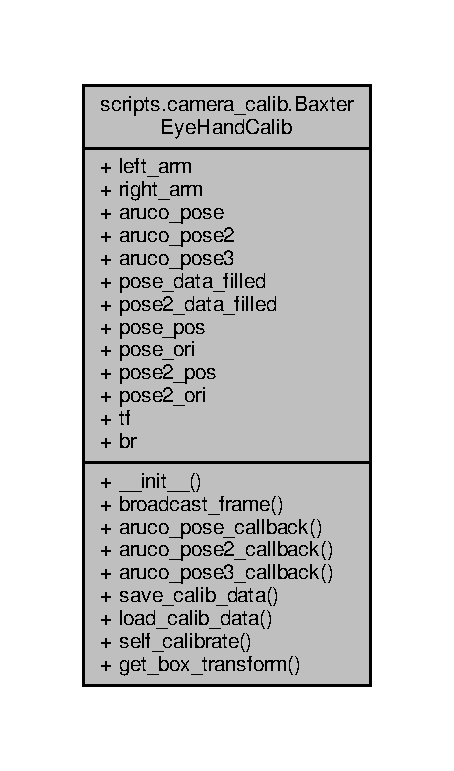
\includegraphics[width=218pt]{classscripts_1_1camera__calib_1_1_baxter_eye_hand_calib__coll__graph}
\end{center}
\end{figure}
\subsection*{Public Member Functions}
\begin{DoxyCompactItemize}
\item 
\hypertarget{classscripts_1_1camera__calib_1_1_baxter_eye_hand_calib_a80e6fdbd3328978e83856bc1f9511904}{def {\bfseries \-\_\-\-\_\-init\-\_\-\-\_\-}}\label{classscripts_1_1camera__calib_1_1_baxter_eye_hand_calib_a80e6fdbd3328978e83856bc1f9511904}

\item 
\hypertarget{classscripts_1_1camera__calib_1_1_baxter_eye_hand_calib_a5e488e63f6aba8960984276bf46df832}{def {\bfseries broadcast\-\_\-frame}}\label{classscripts_1_1camera__calib_1_1_baxter_eye_hand_calib_a5e488e63f6aba8960984276bf46df832}

\item 
\hypertarget{classscripts_1_1camera__calib_1_1_baxter_eye_hand_calib_ab26f80c1371115eda5b2b577597418c8}{def {\bfseries aruco\-\_\-pose\-\_\-callback}}\label{classscripts_1_1camera__calib_1_1_baxter_eye_hand_calib_ab26f80c1371115eda5b2b577597418c8}

\item 
\hypertarget{classscripts_1_1camera__calib_1_1_baxter_eye_hand_calib_a9e60a5b9a52220778599138f43da54c8}{def {\bfseries aruco\-\_\-pose2\-\_\-callback}}\label{classscripts_1_1camera__calib_1_1_baxter_eye_hand_calib_a9e60a5b9a52220778599138f43da54c8}

\item 
\hypertarget{classscripts_1_1camera__calib_1_1_baxter_eye_hand_calib_a9c9358fd48969228d5c8ffc2bc055b04}{def {\bfseries aruco\-\_\-pose3\-\_\-callback}}\label{classscripts_1_1camera__calib_1_1_baxter_eye_hand_calib_a9c9358fd48969228d5c8ffc2bc055b04}

\item 
\hypertarget{classscripts_1_1camera__calib_1_1_baxter_eye_hand_calib_a2b90ecd8fd8ee5cb210e868b2a90997a}{def {\bfseries save\-\_\-calib\-\_\-data}}\label{classscripts_1_1camera__calib_1_1_baxter_eye_hand_calib_a2b90ecd8fd8ee5cb210e868b2a90997a}

\item 
\hypertarget{classscripts_1_1camera__calib_1_1_baxter_eye_hand_calib_aca74cf091daafb370191e195e95b62e6}{def {\bfseries load\-\_\-calib\-\_\-data}}\label{classscripts_1_1camera__calib_1_1_baxter_eye_hand_calib_aca74cf091daafb370191e195e95b62e6}

\item 
\hypertarget{classscripts_1_1camera__calib_1_1_baxter_eye_hand_calib_ad46242daa5c68b20fd1d460c2542d761}{def {\bfseries self\-\_\-calibrate}}\label{classscripts_1_1camera__calib_1_1_baxter_eye_hand_calib_ad46242daa5c68b20fd1d460c2542d761}

\item 
\hypertarget{classscripts_1_1camera__calib_1_1_baxter_eye_hand_calib_abd71ea660f2e0b548c2606cd20f404a4}{def {\bfseries get\-\_\-box\-\_\-transform}}\label{classscripts_1_1camera__calib_1_1_baxter_eye_hand_calib_abd71ea660f2e0b548c2606cd20f404a4}

\end{DoxyCompactItemize}
\subsection*{Public Attributes}
\begin{DoxyCompactItemize}
\item 
\hypertarget{classscripts_1_1camera__calib_1_1_baxter_eye_hand_calib_ad56b37f9835ab1d410a14321d0ccdc7d}{{\bfseries left\-\_\-arm}}\label{classscripts_1_1camera__calib_1_1_baxter_eye_hand_calib_ad56b37f9835ab1d410a14321d0ccdc7d}

\item 
\hypertarget{classscripts_1_1camera__calib_1_1_baxter_eye_hand_calib_a1e8eb78f3692768af3b48ed999bc9cc9}{{\bfseries right\-\_\-arm}}\label{classscripts_1_1camera__calib_1_1_baxter_eye_hand_calib_a1e8eb78f3692768af3b48ed999bc9cc9}

\item 
\hypertarget{classscripts_1_1camera__calib_1_1_baxter_eye_hand_calib_ad568784ea9ac30513293bba1aea2a857}{{\bfseries aruco\-\_\-pose}}\label{classscripts_1_1camera__calib_1_1_baxter_eye_hand_calib_ad568784ea9ac30513293bba1aea2a857}

\item 
\hypertarget{classscripts_1_1camera__calib_1_1_baxter_eye_hand_calib_a286f3e64b708fa5e421081a541112c9b}{{\bfseries aruco\-\_\-pose2}}\label{classscripts_1_1camera__calib_1_1_baxter_eye_hand_calib_a286f3e64b708fa5e421081a541112c9b}

\item 
\hypertarget{classscripts_1_1camera__calib_1_1_baxter_eye_hand_calib_a9b482e44d1f456a7212caf8b04a82623}{{\bfseries aruco\-\_\-pose3}}\label{classscripts_1_1camera__calib_1_1_baxter_eye_hand_calib_a9b482e44d1f456a7212caf8b04a82623}

\item 
\hypertarget{classscripts_1_1camera__calib_1_1_baxter_eye_hand_calib_a4a485c29284a2921e762d4599c736bd1}{{\bfseries pose\-\_\-data\-\_\-filled}}\label{classscripts_1_1camera__calib_1_1_baxter_eye_hand_calib_a4a485c29284a2921e762d4599c736bd1}

\item 
\hypertarget{classscripts_1_1camera__calib_1_1_baxter_eye_hand_calib_ad87ce37e7087b0c8a5219821b4712e27}{{\bfseries pose2\-\_\-data\-\_\-filled}}\label{classscripts_1_1camera__calib_1_1_baxter_eye_hand_calib_ad87ce37e7087b0c8a5219821b4712e27}

\item 
\hypertarget{classscripts_1_1camera__calib_1_1_baxter_eye_hand_calib_ad98e6855ab85a0ddc846282de39cc74f}{{\bfseries pose\-\_\-pos}}\label{classscripts_1_1camera__calib_1_1_baxter_eye_hand_calib_ad98e6855ab85a0ddc846282de39cc74f}

\item 
\hypertarget{classscripts_1_1camera__calib_1_1_baxter_eye_hand_calib_afeed0b6826a0e6dd3362fa84138c06cf}{{\bfseries pose\-\_\-ori}}\label{classscripts_1_1camera__calib_1_1_baxter_eye_hand_calib_afeed0b6826a0e6dd3362fa84138c06cf}

\item 
\hypertarget{classscripts_1_1camera__calib_1_1_baxter_eye_hand_calib_adcb4f9d2feb400ef7ca8bb0672d23ea2}{{\bfseries pose2\-\_\-pos}}\label{classscripts_1_1camera__calib_1_1_baxter_eye_hand_calib_adcb4f9d2feb400ef7ca8bb0672d23ea2}

\item 
\hypertarget{classscripts_1_1camera__calib_1_1_baxter_eye_hand_calib_accdcaa8aa525885e280f8618040a0927}{{\bfseries pose2\-\_\-ori}}\label{classscripts_1_1camera__calib_1_1_baxter_eye_hand_calib_accdcaa8aa525885e280f8618040a0927}

\item 
\hypertarget{classscripts_1_1camera__calib_1_1_baxter_eye_hand_calib_a8c775943efd1fb7730e739366b295027}{{\bfseries tf}}\label{classscripts_1_1camera__calib_1_1_baxter_eye_hand_calib_a8c775943efd1fb7730e739366b295027}

\item 
\hypertarget{classscripts_1_1camera__calib_1_1_baxter_eye_hand_calib_a9d083d71d6425de359b3550c16fc97a6}{{\bfseries br}}\label{classscripts_1_1camera__calib_1_1_baxter_eye_hand_calib_a9d083d71d6425de359b3550c16fc97a6}

\end{DoxyCompactItemize}


The documentation for this class was generated from the following file\-:\begin{DoxyCompactItemize}
\item 
aml\-\_\-calib/scripts/camera\-\_\-calib.\-py\end{DoxyCompactItemize}

\hypertarget{classbaxter__gazebo__plugin_1_1_baxter_gazebo_ros_control_plugin}{}\section{baxter\+\_\+gazebo\+\_\+plugin\+:\+:Baxter\+Gazebo\+Ros\+Control\+Plugin Class Reference}
\label{classbaxter__gazebo__plugin_1_1_baxter_gazebo_ros_control_plugin}\index{baxter\+\_\+gazebo\+\_\+plugin\+::\+Baxter\+Gazebo\+Ros\+Control\+Plugin@{baxter\+\_\+gazebo\+\_\+plugin\+::\+Baxter\+Gazebo\+Ros\+Control\+Plugin}}


Inheritance diagram for baxter\+\_\+gazebo\+\_\+plugin\+:\+:Baxter\+Gazebo\+Ros\+Control\+Plugin\+:
\nopagebreak
\begin{figure}[H]
\begin{center}
\leavevmode
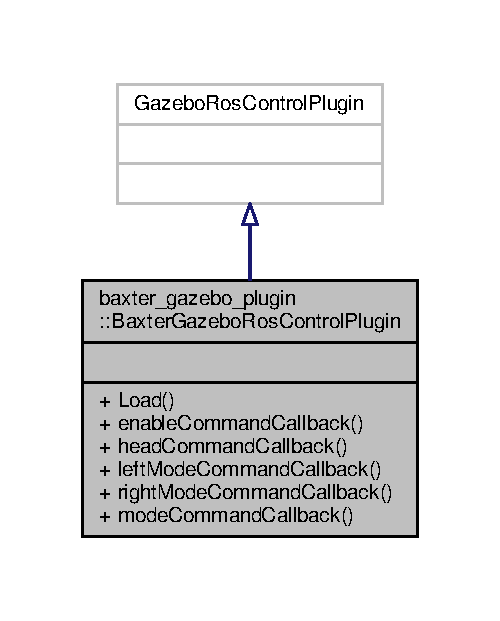
\includegraphics[width=243pt]{classbaxter__gazebo__plugin_1_1_baxter_gazebo_ros_control_plugin__inherit__graph}
\end{center}
\end{figure}


Collaboration diagram for baxter\+\_\+gazebo\+\_\+plugin\+:\+:Baxter\+Gazebo\+Ros\+Control\+Plugin\+:
\nopagebreak
\begin{figure}[H]
\begin{center}
\leavevmode
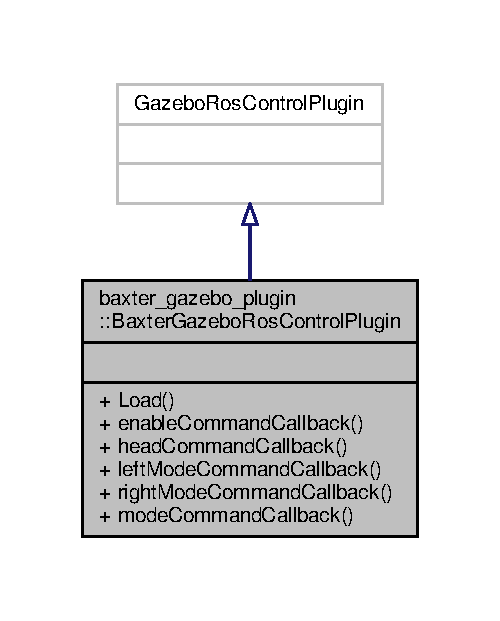
\includegraphics[width=243pt]{classbaxter__gazebo__plugin_1_1_baxter_gazebo_ros_control_plugin__coll__graph}
\end{center}
\end{figure}
\subsection*{Public Member Functions}
\begin{DoxyCompactItemize}
\item 
\hypertarget{classbaxter__gazebo__plugin_1_1_baxter_gazebo_ros_control_plugin_ad18708c5af902c198c114c6908c86d66}{}\label{classbaxter__gazebo__plugin_1_1_baxter_gazebo_ros_control_plugin_ad18708c5af902c198c114c6908c86d66} 
void {\bfseries Load} (gazebo\+::physics\+::\+Model\+Ptr parent, sdf\+::\+Element\+Ptr sdf)
\item 
\hypertarget{classbaxter__gazebo__plugin_1_1_baxter_gazebo_ros_control_plugin_ae142ff05eb7ee5d223939b1ecb41731f}{}\label{classbaxter__gazebo__plugin_1_1_baxter_gazebo_ros_control_plugin_ae142ff05eb7ee5d223939b1ecb41731f} 
void {\bfseries enable\+Command\+Callback} (const baxter\+\_\+core\+\_\+msgs\+::\+Assembly\+State msg)
\item 
\hypertarget{classbaxter__gazebo__plugin_1_1_baxter_gazebo_ros_control_plugin_abcbb5c7e3d26eb2dadfd03de5070ba47}{}\label{classbaxter__gazebo__plugin_1_1_baxter_gazebo_ros_control_plugin_abcbb5c7e3d26eb2dadfd03de5070ba47} 
void {\bfseries head\+Command\+Callback} (const baxter\+\_\+core\+\_\+msgs\+::\+Head\+Pan\+Command msg)
\item 
\hypertarget{classbaxter__gazebo__plugin_1_1_baxter_gazebo_ros_control_plugin_aad16fe48445d9dd9b21d3615034e2f37}{}\label{classbaxter__gazebo__plugin_1_1_baxter_gazebo_ros_control_plugin_aad16fe48445d9dd9b21d3615034e2f37} 
void {\bfseries left\+Mode\+Command\+Callback} (const baxter\+\_\+core\+\_\+msgs\+::\+Joint\+Command\+Const\+Ptr \&msg)
\item 
\hypertarget{classbaxter__gazebo__plugin_1_1_baxter_gazebo_ros_control_plugin_a5d21bace211533c2ea269e10ff7f63aa}{}\label{classbaxter__gazebo__plugin_1_1_baxter_gazebo_ros_control_plugin_a5d21bace211533c2ea269e10ff7f63aa} 
void {\bfseries right\+Mode\+Command\+Callback} (const baxter\+\_\+core\+\_\+msgs\+::\+Joint\+Command\+Const\+Ptr \&msg)
\item 
void \hyperlink{classbaxter__gazebo__plugin_1_1_baxter_gazebo_ros_control_plugin_aff0207bdb9a7d00b791ce5edc6ee27b9}{mode\+Command\+Callback} (const baxter\+\_\+core\+\_\+msgs\+::\+Joint\+Command\+Const\+Ptr \&msg, const std\+::string \&side)
\end{DoxyCompactItemize}


\subsection{Member Function Documentation}
\hypertarget{classbaxter__gazebo__plugin_1_1_baxter_gazebo_ros_control_plugin_aff0207bdb9a7d00b791ce5edc6ee27b9}{}\label{classbaxter__gazebo__plugin_1_1_baxter_gazebo_ros_control_plugin_aff0207bdb9a7d00b791ce5edc6ee27b9} 
\index{baxter\+\_\+gazebo\+\_\+plugin\+::\+Baxter\+Gazebo\+Ros\+Control\+Plugin@{baxter\+\_\+gazebo\+\_\+plugin\+::\+Baxter\+Gazebo\+Ros\+Control\+Plugin}!mode\+Command\+Callback@{mode\+Command\+Callback}}
\index{mode\+Command\+Callback@{mode\+Command\+Callback}!baxter\+\_\+gazebo\+\_\+plugin\+::\+Baxter\+Gazebo\+Ros\+Control\+Plugin@{baxter\+\_\+gazebo\+\_\+plugin\+::\+Baxter\+Gazebo\+Ros\+Control\+Plugin}}
\subsubsection{\texorpdfstring{mode\+Command\+Callback()}{modeCommandCallback()}}
{\footnotesize\ttfamily void baxter\+\_\+gazebo\+\_\+plugin\+::\+Baxter\+Gazebo\+Ros\+Control\+Plugin\+::mode\+Command\+Callback (\begin{DoxyParamCaption}\item[{const baxter\+\_\+core\+\_\+msgs\+::\+Joint\+Command\+Const\+Ptr \&}]{msg,  }\item[{const std\+::string \&}]{side }\end{DoxyParamCaption})\hspace{0.3cm}{\ttfamily [inline]}}

Switch multiple controllers simultaneously.


\begin{DoxyParams}{Parameters}
{\em start\+\_\+controllers} & A vector of controller names to be started \\
\hline
{\em stop\+\_\+controllers} & A vector of controller names to be stopped \\
\hline
{\em strictness} & How important it is that the requested controllers are started and stopped. The levels are defined in the controller\+\_\+manager\+\_\+msgs/\+Switch\+Controllers service as either {\ttfamily B\+E\+S\+T\+\_\+\+E\+F\+F\+O\+RT} or {\ttfamily S\+T\+R\+I\+CT}. {\ttfamily B\+E\+S\+T\+\_\+\+E\+F\+F\+O\+RT} means that switch\+Controller can still succeed if a non-\/existant controller is requested to be stopped or started.\\
\hline
\end{DoxyParams}


The documentation for this class was generated from the following file\+:\begin{DoxyCompactItemize}
\item 
aml\+\_\+assets/gazebo\+\_\+files/aml\+\_\+baxter\+\_\+gazebo/src/aml\+\_\+baxter\+\_\+gazebo\+\_\+ros\+\_\+control\+\_\+plugin.\+cpp\end{DoxyCompactItemize}

\hypertarget{classaml__ctrl_1_1controllers_1_1os__controllers_1_1os__moveit__baxter__controller_1_1_baxter_move_it_controller}{}\section{aml\+\_\+ctrl.\+controllers.\+os\+\_\+controllers.\+os\+\_\+moveit\+\_\+baxter\+\_\+controller.\+Baxter\+Move\+It\+Controller Class Reference}
\label{classaml__ctrl_1_1controllers_1_1os__controllers_1_1os__moveit__baxter__controller_1_1_baxter_move_it_controller}\index{aml\+\_\+ctrl.\+controllers.\+os\+\_\+controllers.\+os\+\_\+moveit\+\_\+baxter\+\_\+controller.\+Baxter\+Move\+It\+Controller@{aml\+\_\+ctrl.\+controllers.\+os\+\_\+controllers.\+os\+\_\+moveit\+\_\+baxter\+\_\+controller.\+Baxter\+Move\+It\+Controller}}


Collaboration diagram for aml\+\_\+ctrl.\+controllers.\+os\+\_\+controllers.\+os\+\_\+moveit\+\_\+baxter\+\_\+controller.\+Baxter\+Move\+It\+Controller\+:\nopagebreak
\begin{figure}[H]
\begin{center}
\leavevmode
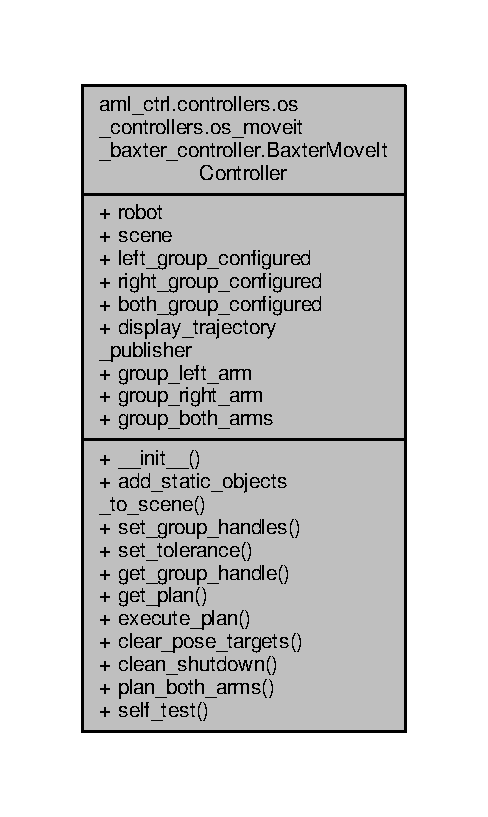
\includegraphics[width=237pt]{classaml__ctrl_1_1controllers_1_1os__controllers_1_1os__moveit__baxter__controller_1_1_baxter_move_it_controller__coll__graph}
\end{center}
\end{figure}
\subsection*{Public Member Functions}
\begin{DoxyCompactItemize}
\item 
\hypertarget{classaml__ctrl_1_1controllers_1_1os__controllers_1_1os__moveit__baxter__controller_1_1_baxter_move_it_controller_a1a84873529afbe9a69e6417b081c69b6}{}\label{classaml__ctrl_1_1controllers_1_1os__controllers_1_1os__moveit__baxter__controller_1_1_baxter_move_it_controller_a1a84873529afbe9a69e6417b081c69b6} 
def {\bfseries \+\_\+\+\_\+init\+\_\+\+\_\+} (self)
\item 
\hypertarget{classaml__ctrl_1_1controllers_1_1os__controllers_1_1os__moveit__baxter__controller_1_1_baxter_move_it_controller_aee42fd2df699bf36bacab48c62a3f835}{}\label{classaml__ctrl_1_1controllers_1_1os__controllers_1_1os__moveit__baxter__controller_1_1_baxter_move_it_controller_aee42fd2df699bf36bacab48c62a3f835} 
def {\bfseries add\+\_\+static\+\_\+objects\+\_\+to\+\_\+scene} (self, limb\+\_\+group=0, obj\+\_\+pos=None, obj\+\_\+ori=None)
\item 
\hypertarget{classaml__ctrl_1_1controllers_1_1os__controllers_1_1os__moveit__baxter__controller_1_1_baxter_move_it_controller_a8654d7c265d7b24cd100f9d48b27009e}{}\label{classaml__ctrl_1_1controllers_1_1os__controllers_1_1os__moveit__baxter__controller_1_1_baxter_move_it_controller_a8654d7c265d7b24cd100f9d48b27009e} 
def {\bfseries set\+\_\+group\+\_\+handles} (self, limb\+\_\+group=1)
\item 
\hypertarget{classaml__ctrl_1_1controllers_1_1os__controllers_1_1os__moveit__baxter__controller_1_1_baxter_move_it_controller_a5c36ba80284c58cd330250fe22df2b5f}{}\label{classaml__ctrl_1_1controllers_1_1os__controllers_1_1os__moveit__baxter__controller_1_1_baxter_move_it_controller_a5c36ba80284c58cd330250fe22df2b5f} 
def {\bfseries set\+\_\+tolerance} (self, group\+\_\+handle, pos\+\_\+tol=0.\+01, ori\+\_\+tol=0.\+01)
\item 
\hypertarget{classaml__ctrl_1_1controllers_1_1os__controllers_1_1os__moveit__baxter__controller_1_1_baxter_move_it_controller_a64def61cb6183744bb7811b12ae44f9d}{}\label{classaml__ctrl_1_1controllers_1_1os__controllers_1_1os__moveit__baxter__controller_1_1_baxter_move_it_controller_a64def61cb6183744bb7811b12ae44f9d} 
def {\bfseries get\+\_\+group\+\_\+handle} (self, limb\+\_\+group=1)
\item 
\hypertarget{classaml__ctrl_1_1controllers_1_1os__controllers_1_1os__moveit__baxter__controller_1_1_baxter_move_it_controller_a7a3f0ed80f28cc25fde582192593294e}{}\label{classaml__ctrl_1_1controllers_1_1os__controllers_1_1os__moveit__baxter__controller_1_1_baxter_move_it_controller_a7a3f0ed80f28cc25fde582192593294e} 
def {\bfseries get\+\_\+plan} (self, limb\+\_\+group, pos, ori, wait\+\_\+time=1.\+5)
\item 
\hypertarget{classaml__ctrl_1_1controllers_1_1os__controllers_1_1os__moveit__baxter__controller_1_1_baxter_move_it_controller_a2b49e5087fb6eaa70c6d13b768fdd164}{}\label{classaml__ctrl_1_1controllers_1_1os__controllers_1_1os__moveit__baxter__controller_1_1_baxter_move_it_controller_a2b49e5087fb6eaa70c6d13b768fdd164} 
def {\bfseries execute\+\_\+plan} (self, limb\+\_\+group, plan, real\+\_\+robot=False)
\item 
\hypertarget{classaml__ctrl_1_1controllers_1_1os__controllers_1_1os__moveit__baxter__controller_1_1_baxter_move_it_controller_ad5a033cc3fe8ed279770142466382764}{}\label{classaml__ctrl_1_1controllers_1_1os__controllers_1_1os__moveit__baxter__controller_1_1_baxter_move_it_controller_ad5a033cc3fe8ed279770142466382764} 
def {\bfseries clear\+\_\+pose\+\_\+targets} (self, limb\+\_\+group=1)
\item 
\hypertarget{classaml__ctrl_1_1controllers_1_1os__controllers_1_1os__moveit__baxter__controller_1_1_baxter_move_it_controller_a775b3416eb7d00d6270e69df81fd9e49}{}\label{classaml__ctrl_1_1controllers_1_1os__controllers_1_1os__moveit__baxter__controller_1_1_baxter_move_it_controller_a775b3416eb7d00d6270e69df81fd9e49} 
def {\bfseries clean\+\_\+shutdown} (self)
\item 
\hypertarget{classaml__ctrl_1_1controllers_1_1os__controllers_1_1os__moveit__baxter__controller_1_1_baxter_move_it_controller_a862572cd81154f514ea5044bf8cd7773}{}\label{classaml__ctrl_1_1controllers_1_1os__controllers_1_1os__moveit__baxter__controller_1_1_baxter_move_it_controller_a862572cd81154f514ea5044bf8cd7773} 
def {\bfseries plan\+\_\+both\+\_\+arms} (self, left\+\_\+pos, left\+\_\+ori, right\+\_\+pos, right\+\_\+ori)
\item 
\hypertarget{classaml__ctrl_1_1controllers_1_1os__controllers_1_1os__moveit__baxter__controller_1_1_baxter_move_it_controller_a76cb945e9e88f0d902e820cf1d1421c4}{}\label{classaml__ctrl_1_1controllers_1_1os__controllers_1_1os__moveit__baxter__controller_1_1_baxter_move_it_controller_a76cb945e9e88f0d902e820cf1d1421c4} 
def {\bfseries self\+\_\+test} (self, limb\+\_\+group=1)
\end{DoxyCompactItemize}
\subsection*{Public Attributes}
\begin{DoxyCompactItemize}
\item 
\hypertarget{classaml__ctrl_1_1controllers_1_1os__controllers_1_1os__moveit__baxter__controller_1_1_baxter_move_it_controller_a1c534361d1c6f82e6e6d0781097410bc}{}\label{classaml__ctrl_1_1controllers_1_1os__controllers_1_1os__moveit__baxter__controller_1_1_baxter_move_it_controller_a1c534361d1c6f82e6e6d0781097410bc} 
{\bfseries robot}
\item 
\hypertarget{classaml__ctrl_1_1controllers_1_1os__controllers_1_1os__moveit__baxter__controller_1_1_baxter_move_it_controller_abde30d477cfd2f39c9a7fe6e1227028b}{}\label{classaml__ctrl_1_1controllers_1_1os__controllers_1_1os__moveit__baxter__controller_1_1_baxter_move_it_controller_abde30d477cfd2f39c9a7fe6e1227028b} 
{\bfseries scene}
\item 
\hypertarget{classaml__ctrl_1_1controllers_1_1os__controllers_1_1os__moveit__baxter__controller_1_1_baxter_move_it_controller_a44ac924f2a51afd683e775fe6dc7baca}{}\label{classaml__ctrl_1_1controllers_1_1os__controllers_1_1os__moveit__baxter__controller_1_1_baxter_move_it_controller_a44ac924f2a51afd683e775fe6dc7baca} 
{\bfseries left\+\_\+group\+\_\+configured}
\item 
\hypertarget{classaml__ctrl_1_1controllers_1_1os__controllers_1_1os__moveit__baxter__controller_1_1_baxter_move_it_controller_a12e7944ade73dc34e96e1bef3949ae58}{}\label{classaml__ctrl_1_1controllers_1_1os__controllers_1_1os__moveit__baxter__controller_1_1_baxter_move_it_controller_a12e7944ade73dc34e96e1bef3949ae58} 
{\bfseries right\+\_\+group\+\_\+configured}
\item 
\hypertarget{classaml__ctrl_1_1controllers_1_1os__controllers_1_1os__moveit__baxter__controller_1_1_baxter_move_it_controller_aa9c8571105d028ff6e64a7cee0d10393}{}\label{classaml__ctrl_1_1controllers_1_1os__controllers_1_1os__moveit__baxter__controller_1_1_baxter_move_it_controller_aa9c8571105d028ff6e64a7cee0d10393} 
{\bfseries both\+\_\+group\+\_\+configured}
\item 
\hypertarget{classaml__ctrl_1_1controllers_1_1os__controllers_1_1os__moveit__baxter__controller_1_1_baxter_move_it_controller_ae424f29d48a9139e177314a1ec9735e3}{}\label{classaml__ctrl_1_1controllers_1_1os__controllers_1_1os__moveit__baxter__controller_1_1_baxter_move_it_controller_ae424f29d48a9139e177314a1ec9735e3} 
{\bfseries display\+\_\+trajectory\+\_\+publisher}
\item 
\hypertarget{classaml__ctrl_1_1controllers_1_1os__controllers_1_1os__moveit__baxter__controller_1_1_baxter_move_it_controller_a6750fdc448f782cfbd3bf1859c8e2503}{}\label{classaml__ctrl_1_1controllers_1_1os__controllers_1_1os__moveit__baxter__controller_1_1_baxter_move_it_controller_a6750fdc448f782cfbd3bf1859c8e2503} 
{\bfseries group\+\_\+left\+\_\+arm}
\item 
\hypertarget{classaml__ctrl_1_1controllers_1_1os__controllers_1_1os__moveit__baxter__controller_1_1_baxter_move_it_controller_afbc743ae405edc5f8974c7b89732aaa7}{}\label{classaml__ctrl_1_1controllers_1_1os__controllers_1_1os__moveit__baxter__controller_1_1_baxter_move_it_controller_afbc743ae405edc5f8974c7b89732aaa7} 
{\bfseries group\+\_\+right\+\_\+arm}
\item 
\hypertarget{classaml__ctrl_1_1controllers_1_1os__controllers_1_1os__moveit__baxter__controller_1_1_baxter_move_it_controller_a8fa5f00622d9497afe8d8df91a0bbe9f}{}\label{classaml__ctrl_1_1controllers_1_1os__controllers_1_1os__moveit__baxter__controller_1_1_baxter_move_it_controller_a8fa5f00622d9497afe8d8df91a0bbe9f} 
{\bfseries group\+\_\+both\+\_\+arms}
\end{DoxyCompactItemize}


The documentation for this class was generated from the following file\+:\begin{DoxyCompactItemize}
\item 
aml\+\_\+ctrl/src/aml\+\_\+ctrl/controllers/os\+\_\+controllers/os\+\_\+moveit\+\_\+baxter\+\_\+controller.\+py\end{DoxyCompactItemize}

\hypertarget{classaml__robot_1_1bullet_1_1push__world_1_1push__machine_1_1_box_object}{}\section{aml\+\_\+robot.\+bullet.\+push\+\_\+world.\+push\+\_\+machine.\+Box\+Object Class Reference}
\label{classaml__robot_1_1bullet_1_1push__world_1_1push__machine_1_1_box_object}\index{aml\+\_\+robot.\+bullet.\+push\+\_\+world.\+push\+\_\+machine.\+Box\+Object@{aml\+\_\+robot.\+bullet.\+push\+\_\+world.\+push\+\_\+machine.\+Box\+Object}}


Inheritance diagram for aml\+\_\+robot.\+bullet.\+push\+\_\+world.\+push\+\_\+machine.\+Box\+Object\+:
\nopagebreak
\begin{figure}[H]
\begin{center}
\leavevmode
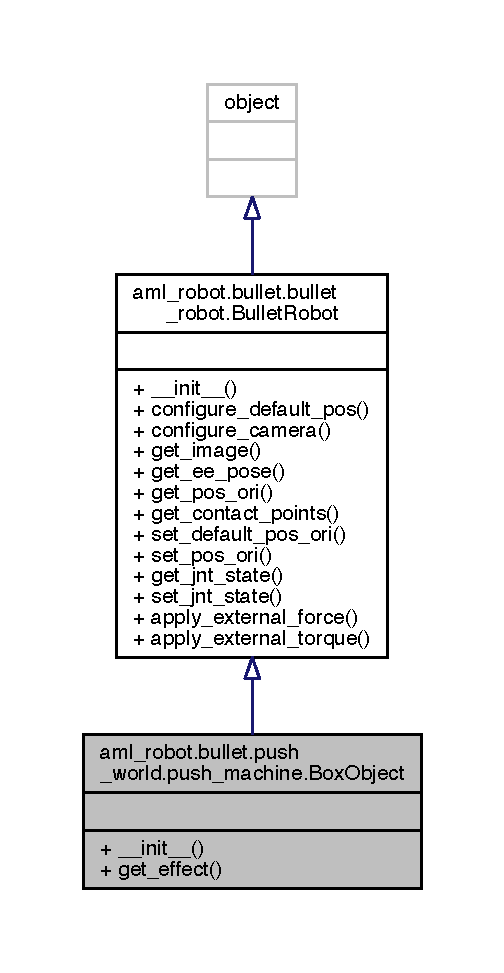
\includegraphics[width=242pt]{classaml__robot_1_1bullet_1_1push__world_1_1push__machine_1_1_box_object__inherit__graph}
\end{center}
\end{figure}


Collaboration diagram for aml\+\_\+robot.\+bullet.\+push\+\_\+world.\+push\+\_\+machine.\+Box\+Object\+:
\nopagebreak
\begin{figure}[H]
\begin{center}
\leavevmode
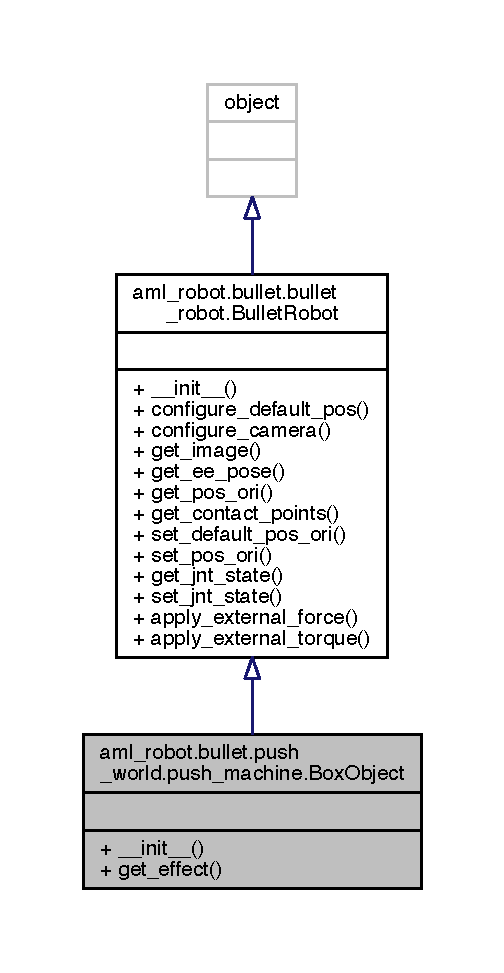
\includegraphics[width=242pt]{classaml__robot_1_1bullet_1_1push__world_1_1push__machine_1_1_box_object__coll__graph}
\end{center}
\end{figure}
\subsection*{Public Member Functions}
\begin{DoxyCompactItemize}
\item 
\hypertarget{classaml__robot_1_1bullet_1_1push__world_1_1push__machine_1_1_box_object_a6176168fbcfdc9c0c09808bf93e01e78}{}\label{classaml__robot_1_1bullet_1_1push__world_1_1push__machine_1_1_box_object_a6176168fbcfdc9c0c09808bf93e01e78} 
def {\bfseries \+\_\+\+\_\+init\+\_\+\+\_\+} (self, box\+\_\+id)
\item 
\hypertarget{classaml__robot_1_1bullet_1_1push__world_1_1push__machine_1_1_box_object_afaf0ea1787cdeda8b5266f9a1d37e723}{}\label{classaml__robot_1_1bullet_1_1push__world_1_1push__machine_1_1_box_object_afaf0ea1787cdeda8b5266f9a1d37e723} 
def {\bfseries get\+\_\+effect} (self)
\end{DoxyCompactItemize}


The documentation for this class was generated from the following file\+:\begin{DoxyCompactItemize}
\item 
aml\+\_\+robot/src/aml\+\_\+robot/bullet/push\+\_\+world/push\+\_\+machine.\+py\end{DoxyCompactItemize}

\hypertarget{classaml__robot_1_1mujoco_1_1push__world_1_1collect__push__data__sim_1_1_box_object}{\section{aml\-\_\-robot.\-mujoco.\-push\-\_\-world.\-collect\-\_\-push\-\_\-data\-\_\-sim.\-Box\-Object Class Reference}
\label{classaml__robot_1_1mujoco_1_1push__world_1_1collect__push__data__sim_1_1_box_object}\index{aml\-\_\-robot.\-mujoco.\-push\-\_\-world.\-collect\-\_\-push\-\_\-data\-\_\-sim.\-Box\-Object@{aml\-\_\-robot.\-mujoco.\-push\-\_\-world.\-collect\-\_\-push\-\_\-data\-\_\-sim.\-Box\-Object}}
}


Collaboration diagram for aml\-\_\-robot.\-mujoco.\-push\-\_\-world.\-collect\-\_\-push\-\_\-data\-\_\-sim.\-Box\-Object\-:
\nopagebreak
\begin{figure}[H]
\begin{center}
\leavevmode
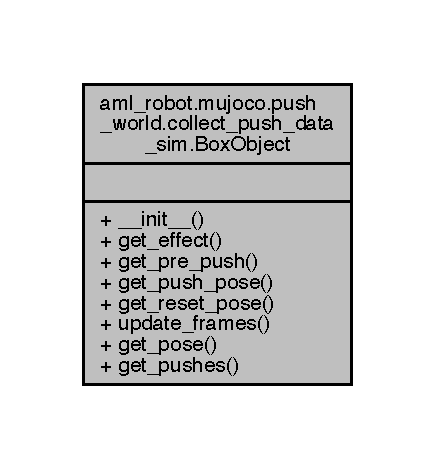
\includegraphics[width=206pt]{classaml__robot_1_1mujoco_1_1push__world_1_1collect__push__data__sim_1_1_box_object__coll__graph}
\end{center}
\end{figure}
\subsection*{Public Member Functions}
\begin{DoxyCompactItemize}
\item 
\hypertarget{classaml__robot_1_1mujoco_1_1push__world_1_1collect__push__data__sim_1_1_box_object_a6fe25f4e34ec4acf176a141e901ffecd}{def {\bfseries \-\_\-\-\_\-init\-\_\-\-\_\-}}\label{classaml__robot_1_1mujoco_1_1push__world_1_1collect__push__data__sim_1_1_box_object_a6fe25f4e34ec4acf176a141e901ffecd}

\item 
\hypertarget{classaml__robot_1_1mujoco_1_1push__world_1_1collect__push__data__sim_1_1_box_object_a720e24b1573d4d5f069da8eb68cbec38}{def {\bfseries get\-\_\-effect}}\label{classaml__robot_1_1mujoco_1_1push__world_1_1collect__push__data__sim_1_1_box_object_a720e24b1573d4d5f069da8eb68cbec38}

\item 
\hypertarget{classaml__robot_1_1mujoco_1_1push__world_1_1collect__push__data__sim_1_1_box_object_a1cd7b6ef72aa2bff61a2743cf9911a53}{def {\bfseries get\-\_\-pre\-\_\-push}}\label{classaml__robot_1_1mujoco_1_1push__world_1_1collect__push__data__sim_1_1_box_object_a1cd7b6ef72aa2bff61a2743cf9911a53}

\item 
\hypertarget{classaml__robot_1_1mujoco_1_1push__world_1_1collect__push__data__sim_1_1_box_object_a67831e80db6470538caa2443fb49cc44}{def {\bfseries get\-\_\-push\-\_\-pose}}\label{classaml__robot_1_1mujoco_1_1push__world_1_1collect__push__data__sim_1_1_box_object_a67831e80db6470538caa2443fb49cc44}

\item 
\hypertarget{classaml__robot_1_1mujoco_1_1push__world_1_1collect__push__data__sim_1_1_box_object_a3ecfa0ceeba774ab9b138a1519596aa8}{def {\bfseries get\-\_\-reset\-\_\-pose}}\label{classaml__robot_1_1mujoco_1_1push__world_1_1collect__push__data__sim_1_1_box_object_a3ecfa0ceeba774ab9b138a1519596aa8}

\item 
\hypertarget{classaml__robot_1_1mujoco_1_1push__world_1_1collect__push__data__sim_1_1_box_object_a02bfb0f0353d6fbb4fc0b776fe74e3ad}{def {\bfseries update\-\_\-frames}}\label{classaml__robot_1_1mujoco_1_1push__world_1_1collect__push__data__sim_1_1_box_object_a02bfb0f0353d6fbb4fc0b776fe74e3ad}

\item 
\hypertarget{classaml__robot_1_1mujoco_1_1push__world_1_1collect__push__data__sim_1_1_box_object_a08e04c4023ce3d917c1c41be1b5ba7c4}{def {\bfseries get\-\_\-pose}}\label{classaml__robot_1_1mujoco_1_1push__world_1_1collect__push__data__sim_1_1_box_object_a08e04c4023ce3d917c1c41be1b5ba7c4}

\item 
\hypertarget{classaml__robot_1_1mujoco_1_1push__world_1_1collect__push__data__sim_1_1_box_object_af61b690b7974ec13358052da7c34267b}{def {\bfseries get\-\_\-pushes}}\label{classaml__robot_1_1mujoco_1_1push__world_1_1collect__push__data__sim_1_1_box_object_af61b690b7974ec13358052da7c34267b}

\end{DoxyCompactItemize}


The documentation for this class was generated from the following file\-:\begin{DoxyCompactItemize}
\item 
aml\-\_\-robot/src/aml\-\_\-robot/mujoco/push\-\_\-world/collect\-\_\-push\-\_\-data\-\_\-sim.\-py\end{DoxyCompactItemize}

\hypertarget{classaml__data__collec__utils_1_1box__object_1_1_box_object}{\section{aml\-\_\-data\-\_\-collec\-\_\-utils.\-box\-\_\-object.\-Box\-Object Class Reference}
\label{classaml__data__collec__utils_1_1box__object_1_1_box_object}\index{aml\-\_\-data\-\_\-collec\-\_\-utils.\-box\-\_\-object.\-Box\-Object@{aml\-\_\-data\-\_\-collec\-\_\-utils.\-box\-\_\-object.\-Box\-Object}}
}


Inheritance diagram for aml\-\_\-data\-\_\-collec\-\_\-utils.\-box\-\_\-object.\-Box\-Object\-:
\nopagebreak
\begin{figure}[H]
\begin{center}
\leavevmode
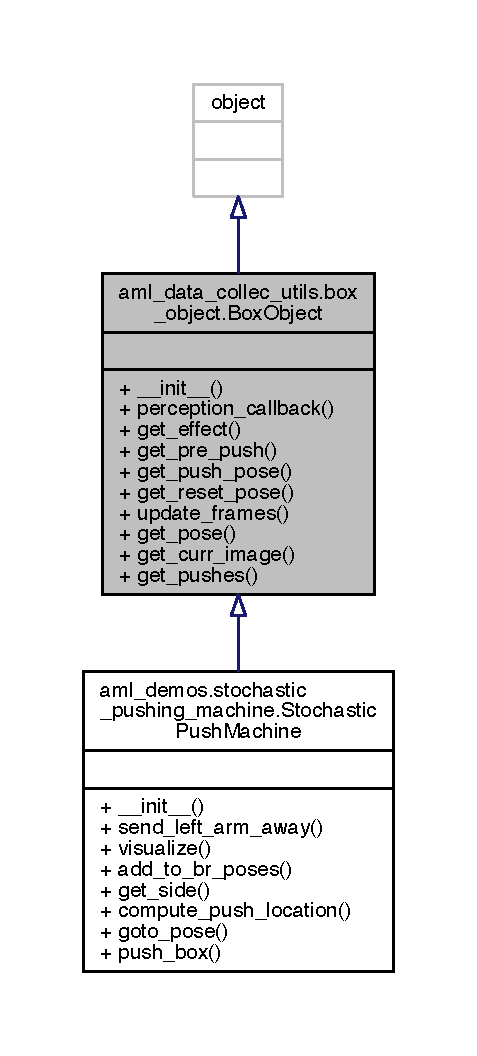
\includegraphics[width=350pt]{classaml__data__collec__utils_1_1box__object_1_1_box_object__inherit__graph}
\end{center}
\end{figure}


Collaboration diagram for aml\-\_\-data\-\_\-collec\-\_\-utils.\-box\-\_\-object.\-Box\-Object\-:
\nopagebreak
\begin{figure}[H]
\begin{center}
\leavevmode
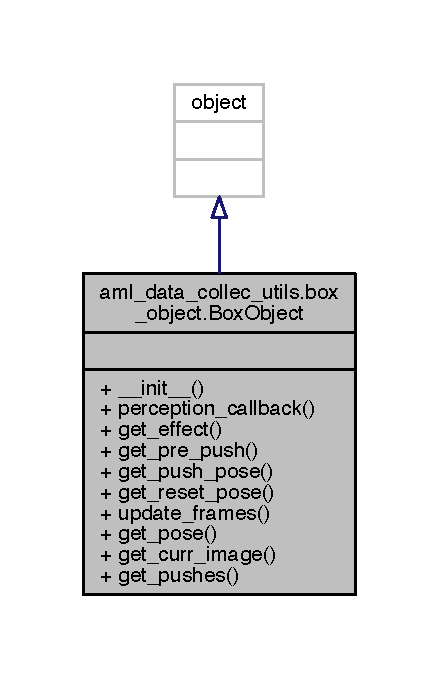
\includegraphics[width=208pt]{classaml__data__collec__utils_1_1box__object_1_1_box_object__coll__graph}
\end{center}
\end{figure}
\subsection*{Public Member Functions}
\begin{DoxyCompactItemize}
\item 
\hypertarget{classaml__data__collec__utils_1_1box__object_1_1_box_object_a0b113ad91ae9191e5f9b22be92b3ac6a}{def {\bfseries \-\_\-\-\_\-init\-\_\-\-\_\-}}\label{classaml__data__collec__utils_1_1box__object_1_1_box_object_a0b113ad91ae9191e5f9b22be92b3ac6a}

\item 
\hypertarget{classaml__data__collec__utils_1_1box__object_1_1_box_object_a9f0b232db9ba73d8cbfdbcfad56ea1b6}{def {\bfseries get\-\_\-effect}}\label{classaml__data__collec__utils_1_1box__object_1_1_box_object_a9f0b232db9ba73d8cbfdbcfad56ea1b6}

\item 
\hypertarget{classaml__data__collec__utils_1_1box__object_1_1_box_object_ac0083e59dc6b79f6f57feaaf3352b30c}{def {\bfseries get\-\_\-pre\-\_\-push}}\label{classaml__data__collec__utils_1_1box__object_1_1_box_object_ac0083e59dc6b79f6f57feaaf3352b30c}

\item 
\hypertarget{classaml__data__collec__utils_1_1box__object_1_1_box_object_a9953fcbc78eb41c18a3876e21097e65f}{def {\bfseries get\-\_\-push\-\_\-pose}}\label{classaml__data__collec__utils_1_1box__object_1_1_box_object_a9953fcbc78eb41c18a3876e21097e65f}

\item 
\hypertarget{classaml__data__collec__utils_1_1box__object_1_1_box_object_a3422f8905c4bb9e15d6af519645f8ccc}{def {\bfseries get\-\_\-reset\-\_\-pose}}\label{classaml__data__collec__utils_1_1box__object_1_1_box_object_a3422f8905c4bb9e15d6af519645f8ccc}

\item 
\hypertarget{classaml__data__collec__utils_1_1box__object_1_1_box_object_ab476197b5c0b40ca1276959cf2f53c97}{def {\bfseries update\-\_\-frames}}\label{classaml__data__collec__utils_1_1box__object_1_1_box_object_ab476197b5c0b40ca1276959cf2f53c97}

\item 
\hypertarget{classaml__data__collec__utils_1_1box__object_1_1_box_object_a9735855fbf5e69e61a921bb6c40d307d}{def {\bfseries get\-\_\-pose}}\label{classaml__data__collec__utils_1_1box__object_1_1_box_object_a9735855fbf5e69e61a921bb6c40d307d}

\item 
\hypertarget{classaml__data__collec__utils_1_1box__object_1_1_box_object_a7d9d988a7607d7ff4b7048542a0c37b3}{def {\bfseries get\-\_\-curr\-\_\-image}}\label{classaml__data__collec__utils_1_1box__object_1_1_box_object_a7d9d988a7607d7ff4b7048542a0c37b3}

\item 
\hypertarget{classaml__data__collec__utils_1_1box__object_1_1_box_object_a7483c6c349ad6fdee4ef76c01bb0cea6}{def {\bfseries get\-\_\-box\-\_\-state}}\label{classaml__data__collec__utils_1_1box__object_1_1_box_object_a7483c6c349ad6fdee4ef76c01bb0cea6}

\item 
\hypertarget{classaml__data__collec__utils_1_1box__object_1_1_box_object_a88af2c9d0a9501750921c75ccc613b55}{def {\bfseries get\-\_\-push}}\label{classaml__data__collec__utils_1_1box__object_1_1_box_object_a88af2c9d0a9501750921c75ccc613b55}

\item 
\hypertarget{classaml__data__collec__utils_1_1box__object_1_1_box_object_aa3824a2b91c66708d28b51d3bdc4e409}{def {\bfseries get\-\_\-pushes}}\label{classaml__data__collec__utils_1_1box__object_1_1_box_object_aa3824a2b91c66708d28b51d3bdc4e409}

\end{DoxyCompactItemize}


The documentation for this class was generated from the following file\-:\begin{DoxyCompactItemize}
\item 
aml\-\_\-data\-\_\-collec\-\_\-utils/src/aml\-\_\-data\-\_\-collec\-\_\-utils/box\-\_\-object.\-py\end{DoxyCompactItemize}

\hypertarget{classaml__robot_1_1bullet_1_1bullet__robot_1_1_bullet_robot}{\section{aml\-\_\-robot.\-bullet.\-bullet\-\_\-robot.\-Bullet\-Robot Class Reference}
\label{classaml__robot_1_1bullet_1_1bullet__robot_1_1_bullet_robot}\index{aml\-\_\-robot.\-bullet.\-bullet\-\_\-robot.\-Bullet\-Robot@{aml\-\_\-robot.\-bullet.\-bullet\-\_\-robot.\-Bullet\-Robot}}
}


Inheritance diagram for aml\-\_\-robot.\-bullet.\-bullet\-\_\-robot.\-Bullet\-Robot\-:
\nopagebreak
\begin{figure}[H]
\begin{center}
\leavevmode
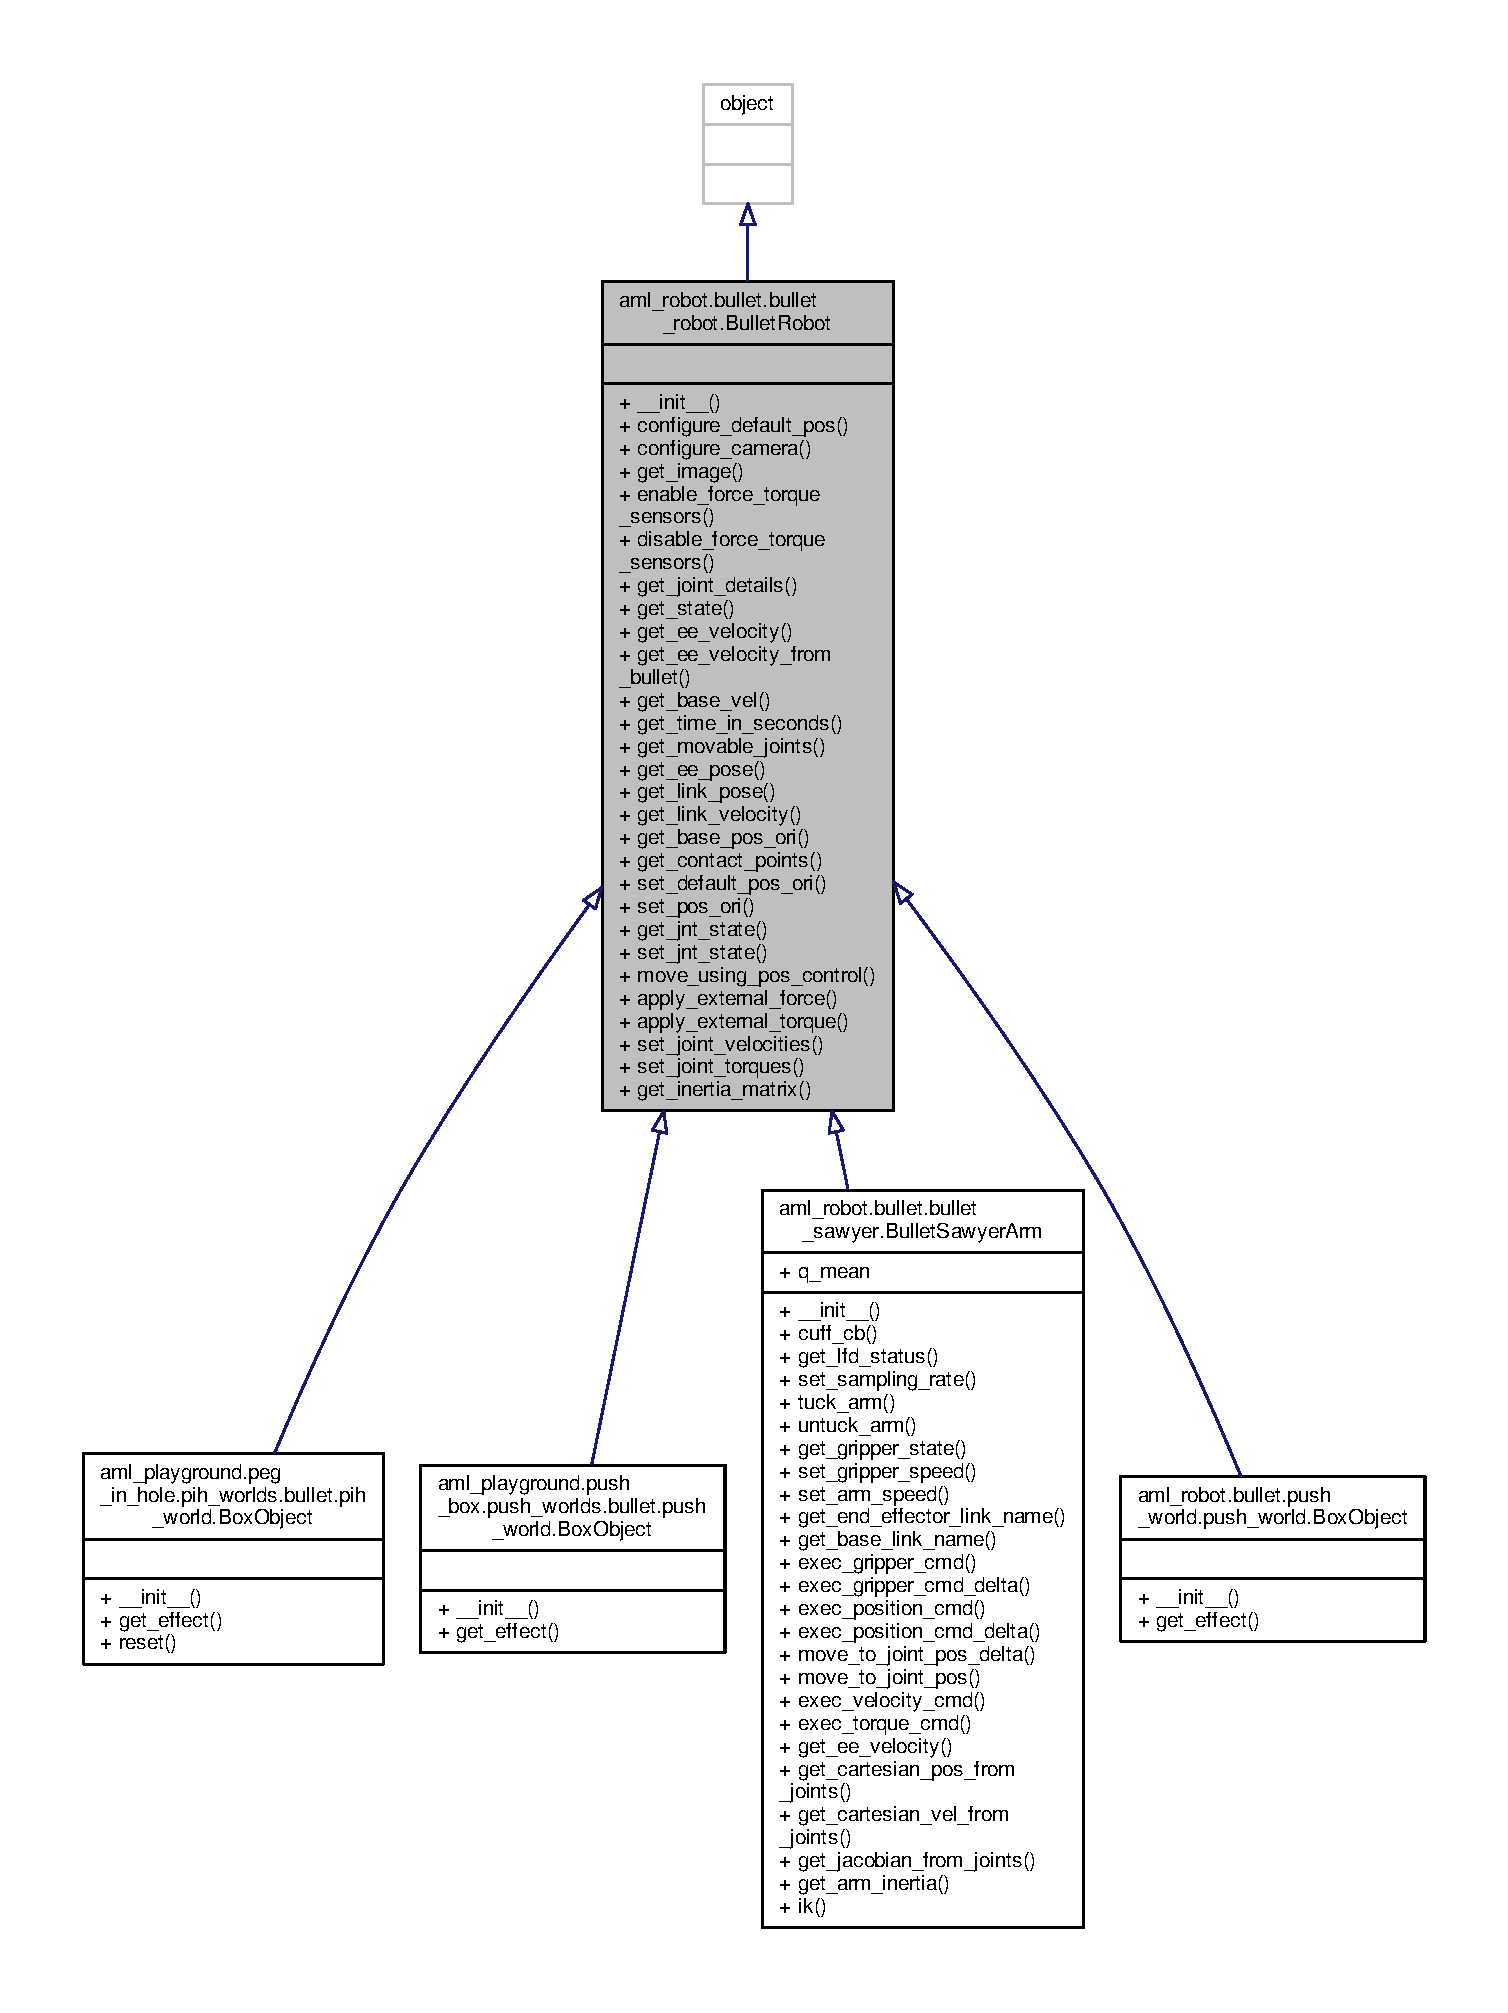
\includegraphics[width=350pt]{classaml__robot_1_1bullet_1_1bullet__robot_1_1_bullet_robot__inherit__graph}
\end{center}
\end{figure}


Collaboration diagram for aml\-\_\-robot.\-bullet.\-bullet\-\_\-robot.\-Bullet\-Robot\-:
\nopagebreak
\begin{figure}[H]
\begin{center}
\leavevmode
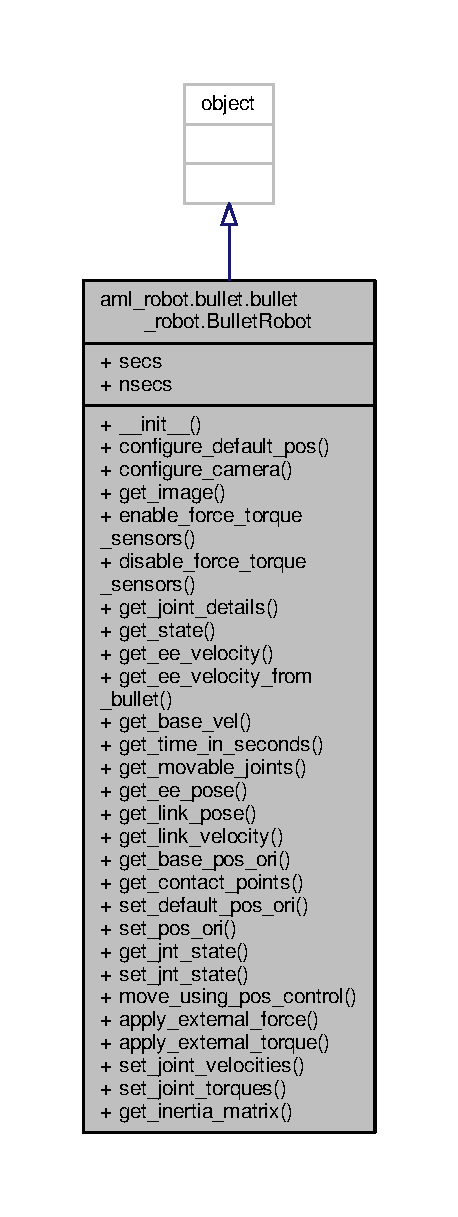
\includegraphics[height=550pt]{classaml__robot_1_1bullet_1_1bullet__robot_1_1_bullet_robot__coll__graph}
\end{center}
\end{figure}
\subsection*{Public Member Functions}
\begin{DoxyCompactItemize}
\item 
\hypertarget{classaml__robot_1_1bullet_1_1bullet__robot_1_1_bullet_robot_a6d7233ae89986285907afa4ab28a405f}{def {\bfseries \-\_\-\-\_\-init\-\_\-\-\_\-}}\label{classaml__robot_1_1bullet_1_1bullet__robot_1_1_bullet_robot_a6d7233ae89986285907afa4ab28a405f}

\item 
\hypertarget{classaml__robot_1_1bullet_1_1bullet__robot_1_1_bullet_robot_a709c2b87512124c09ba59986d5861f3e}{def {\bfseries configure\-\_\-default\-\_\-pos}}\label{classaml__robot_1_1bullet_1_1bullet__robot_1_1_bullet_robot_a709c2b87512124c09ba59986d5861f3e}

\item 
\hypertarget{classaml__robot_1_1bullet_1_1bullet__robot_1_1_bullet_robot_af5a32ad6a5599989c44de85c9913d7c4}{def {\bfseries configure\-\_\-camera}}\label{classaml__robot_1_1bullet_1_1bullet__robot_1_1_bullet_robot_af5a32ad6a5599989c44de85c9913d7c4}

\item 
\hypertarget{classaml__robot_1_1bullet_1_1bullet__robot_1_1_bullet_robot_af647a35802a8587bc7deb67967f68dea}{def {\bfseries get\-\_\-image}}\label{classaml__robot_1_1bullet_1_1bullet__robot_1_1_bullet_robot_af647a35802a8587bc7deb67967f68dea}

\item 
\hypertarget{classaml__robot_1_1bullet_1_1bullet__robot_1_1_bullet_robot_aa4e849e7cff7651983107c04c07ed152}{def {\bfseries enable\-\_\-force\-\_\-torque\-\_\-sensors}}\label{classaml__robot_1_1bullet_1_1bullet__robot_1_1_bullet_robot_aa4e849e7cff7651983107c04c07ed152}

\item 
\hypertarget{classaml__robot_1_1bullet_1_1bullet__robot_1_1_bullet_robot_a4aed842aa5f349071bde6acb44e04a02}{def {\bfseries disable\-\_\-force\-\_\-torque\-\_\-sensors}}\label{classaml__robot_1_1bullet_1_1bullet__robot_1_1_bullet_robot_a4aed842aa5f349071bde6acb44e04a02}

\item 
\hypertarget{classaml__robot_1_1bullet_1_1bullet__robot_1_1_bullet_robot_ab37105f9badd89b4d9c84fdea6287a4a}{def {\bfseries get\-\_\-joint\-\_\-details}}\label{classaml__robot_1_1bullet_1_1bullet__robot_1_1_bullet_robot_ab37105f9badd89b4d9c84fdea6287a4a}

\item 
\hypertarget{classaml__robot_1_1bullet_1_1bullet__robot_1_1_bullet_robot_a331fdaea2b357ca6bb56234f32f56916}{def {\bfseries get\-\_\-state}}\label{classaml__robot_1_1bullet_1_1bullet__robot_1_1_bullet_robot_a331fdaea2b357ca6bb56234f32f56916}

\item 
\hypertarget{classaml__robot_1_1bullet_1_1bullet__robot_1_1_bullet_robot_a003eb9e5644bf58183d21b2b35f1b538}{def {\bfseries get\-\_\-ee\-\_\-velocity}}\label{classaml__robot_1_1bullet_1_1bullet__robot_1_1_bullet_robot_a003eb9e5644bf58183d21b2b35f1b538}

\item 
\hypertarget{classaml__robot_1_1bullet_1_1bullet__robot_1_1_bullet_robot_ad0a44c6fccb87f7d6da9e891a22c1201}{def {\bfseries get\-\_\-ee\-\_\-velocity\-\_\-from\-\_\-bullet}}\label{classaml__robot_1_1bullet_1_1bullet__robot_1_1_bullet_robot_ad0a44c6fccb87f7d6da9e891a22c1201}

\item 
\hypertarget{classaml__robot_1_1bullet_1_1bullet__robot_1_1_bullet_robot_a01a4a77b03ccf152b749bce7e0228de1}{def {\bfseries get\-\_\-base\-\_\-vel}}\label{classaml__robot_1_1bullet_1_1bullet__robot_1_1_bullet_robot_a01a4a77b03ccf152b749bce7e0228de1}

\item 
\hypertarget{classaml__robot_1_1bullet_1_1bullet__robot_1_1_bullet_robot_a192a909b026c4620c2cb6b2a104c9aad}{def {\bfseries get\-\_\-time\-\_\-in\-\_\-seconds}}\label{classaml__robot_1_1bullet_1_1bullet__robot_1_1_bullet_robot_a192a909b026c4620c2cb6b2a104c9aad}

\item 
\hypertarget{classaml__robot_1_1bullet_1_1bullet__robot_1_1_bullet_robot_ae4835535a8930d9c16b5c0c3ce1b6a61}{def {\bfseries get\-\_\-movable\-\_\-joints}}\label{classaml__robot_1_1bullet_1_1bullet__robot_1_1_bullet_robot_ae4835535a8930d9c16b5c0c3ce1b6a61}

\item 
\hypertarget{classaml__robot_1_1bullet_1_1bullet__robot_1_1_bullet_robot_a77aae9137ce2c225edf6c956384e384f}{def {\bfseries get\-\_\-ee\-\_\-pose}}\label{classaml__robot_1_1bullet_1_1bullet__robot_1_1_bullet_robot_a77aae9137ce2c225edf6c956384e384f}

\item 
\hypertarget{classaml__robot_1_1bullet_1_1bullet__robot_1_1_bullet_robot_a6cf2000eca42e7cecdb7da1397452a63}{def {\bfseries get\-\_\-link\-\_\-pose}}\label{classaml__robot_1_1bullet_1_1bullet__robot_1_1_bullet_robot_a6cf2000eca42e7cecdb7da1397452a63}

\item 
\hypertarget{classaml__robot_1_1bullet_1_1bullet__robot_1_1_bullet_robot_acfb7e09561b5ef801e246bbdbb8fb1c0}{def {\bfseries get\-\_\-link\-\_\-velocity}}\label{classaml__robot_1_1bullet_1_1bullet__robot_1_1_bullet_robot_acfb7e09561b5ef801e246bbdbb8fb1c0}

\item 
\hypertarget{classaml__robot_1_1bullet_1_1bullet__robot_1_1_bullet_robot_a7474f982433aa1db27645da305931c1a}{def {\bfseries get\-\_\-base\-\_\-pos\-\_\-ori}}\label{classaml__robot_1_1bullet_1_1bullet__robot_1_1_bullet_robot_a7474f982433aa1db27645da305931c1a}

\item 
\hypertarget{classaml__robot_1_1bullet_1_1bullet__robot_1_1_bullet_robot_ad604789d11e1c674001cbfb7abd1d16d}{def {\bfseries get\-\_\-contact\-\_\-points}}\label{classaml__robot_1_1bullet_1_1bullet__robot_1_1_bullet_robot_ad604789d11e1c674001cbfb7abd1d16d}

\item 
\hypertarget{classaml__robot_1_1bullet_1_1bullet__robot_1_1_bullet_robot_aee8d45c207fc0d9883560ee231001188}{def {\bfseries set\-\_\-default\-\_\-pos\-\_\-ori}}\label{classaml__robot_1_1bullet_1_1bullet__robot_1_1_bullet_robot_aee8d45c207fc0d9883560ee231001188}

\item 
\hypertarget{classaml__robot_1_1bullet_1_1bullet__robot_1_1_bullet_robot_a9a5f1f2cc810da7412e7daf368567bc2}{def {\bfseries set\-\_\-pos\-\_\-ori}}\label{classaml__robot_1_1bullet_1_1bullet__robot_1_1_bullet_robot_a9a5f1f2cc810da7412e7daf368567bc2}

\item 
\hypertarget{classaml__robot_1_1bullet_1_1bullet__robot_1_1_bullet_robot_a4baea03b7ef7308e4e3503f01aec9c95}{def {\bfseries get\-\_\-jnt\-\_\-state}}\label{classaml__robot_1_1bullet_1_1bullet__robot_1_1_bullet_robot_a4baea03b7ef7308e4e3503f01aec9c95}

\item 
\hypertarget{classaml__robot_1_1bullet_1_1bullet__robot_1_1_bullet_robot_a38011296832f23eb67baf1659e4a9099}{def {\bfseries set\-\_\-jnt\-\_\-state}}\label{classaml__robot_1_1bullet_1_1bullet__robot_1_1_bullet_robot_a38011296832f23eb67baf1659e4a9099}

\item 
\hypertarget{classaml__robot_1_1bullet_1_1bullet__robot_1_1_bullet_robot_ab6e829310089354ebdc3a92c326dd6c3}{def {\bfseries move\-\_\-using\-\_\-pos\-\_\-control}}\label{classaml__robot_1_1bullet_1_1bullet__robot_1_1_bullet_robot_ab6e829310089354ebdc3a92c326dd6c3}

\item 
\hypertarget{classaml__robot_1_1bullet_1_1bullet__robot_1_1_bullet_robot_a16cd3128a33a669b715262a6566e7412}{def {\bfseries apply\-\_\-external\-\_\-force}}\label{classaml__robot_1_1bullet_1_1bullet__robot_1_1_bullet_robot_a16cd3128a33a669b715262a6566e7412}

\item 
\hypertarget{classaml__robot_1_1bullet_1_1bullet__robot_1_1_bullet_robot_acb39fd8e2a984ee5bf7b2d4f22d3cfcf}{def {\bfseries apply\-\_\-external\-\_\-torque}}\label{classaml__robot_1_1bullet_1_1bullet__robot_1_1_bullet_robot_acb39fd8e2a984ee5bf7b2d4f22d3cfcf}

\item 
\hypertarget{classaml__robot_1_1bullet_1_1bullet__robot_1_1_bullet_robot_a6887b7c121e80a302f9e77dc94c9c39a}{def {\bfseries set\-\_\-joint\-\_\-velocities}}\label{classaml__robot_1_1bullet_1_1bullet__robot_1_1_bullet_robot_a6887b7c121e80a302f9e77dc94c9c39a}

\item 
\hypertarget{classaml__robot_1_1bullet_1_1bullet__robot_1_1_bullet_robot_ae26eef83ee4b61ab862e9c5221cce502}{def {\bfseries set\-\_\-joint\-\_\-torques}}\label{classaml__robot_1_1bullet_1_1bullet__robot_1_1_bullet_robot_ae26eef83ee4b61ab862e9c5221cce502}

\item 
\hypertarget{classaml__robot_1_1bullet_1_1bullet__robot_1_1_bullet_robot_aa6ede6bc549404e2b75464bec59714c7}{def {\bfseries get\-\_\-inertia\-\_\-matrix}}\label{classaml__robot_1_1bullet_1_1bullet__robot_1_1_bullet_robot_aa6ede6bc549404e2b75464bec59714c7}

\end{DoxyCompactItemize}


The documentation for this class was generated from the following file\-:\begin{DoxyCompactItemize}
\item 
aml\-\_\-robot/src/aml\-\_\-robot/bullet/bullet\-\_\-robot.\-py\end{DoxyCompactItemize}

\hypertarget{classaml__perception_1_1camera__sensor_1_1_camera_sensor}{\section{aml\-\_\-perception.\-camera\-\_\-sensor.\-Camera\-Sensor Class Reference}
\label{classaml__perception_1_1camera__sensor_1_1_camera_sensor}\index{aml\-\_\-perception.\-camera\-\_\-sensor.\-Camera\-Sensor@{aml\-\_\-perception.\-camera\-\_\-sensor.\-Camera\-Sensor}}
}


Inheritance diagram for aml\-\_\-perception.\-camera\-\_\-sensor.\-Camera\-Sensor\-:
\nopagebreak
\begin{figure}[H]
\begin{center}
\leavevmode
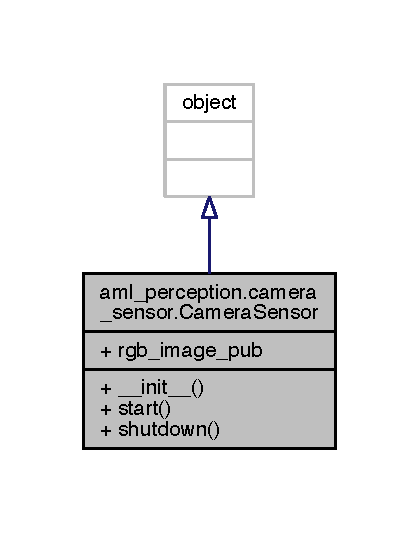
\includegraphics[width=198pt]{classaml__perception_1_1camera__sensor_1_1_camera_sensor__inherit__graph}
\end{center}
\end{figure}


Collaboration diagram for aml\-\_\-perception.\-camera\-\_\-sensor.\-Camera\-Sensor\-:
\nopagebreak
\begin{figure}[H]
\begin{center}
\leavevmode
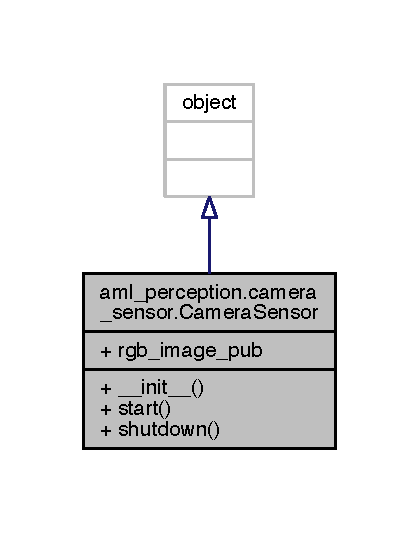
\includegraphics[width=198pt]{classaml__perception_1_1camera__sensor_1_1_camera_sensor__coll__graph}
\end{center}
\end{figure}
\subsection*{Public Member Functions}
\begin{DoxyCompactItemize}
\item 
\hypertarget{classaml__perception_1_1camera__sensor_1_1_camera_sensor_a21adf5c3740d47e8fb55c932e924618d}{def {\bfseries \-\_\-\-\_\-init\-\_\-\-\_\-}}\label{classaml__perception_1_1camera__sensor_1_1_camera_sensor_a21adf5c3740d47e8fb55c932e924618d}

\item 
\hypertarget{classaml__perception_1_1camera__sensor_1_1_camera_sensor_a08a06c82a0528c0462a49ec93db4dc0b}{def {\bfseries start}}\label{classaml__perception_1_1camera__sensor_1_1_camera_sensor_a08a06c82a0528c0462a49ec93db4dc0b}

\item 
\hypertarget{classaml__perception_1_1camera__sensor_1_1_camera_sensor_a95227671ed4cf14c09493d81bc619ea7}{def {\bfseries shutdown}}\label{classaml__perception_1_1camera__sensor_1_1_camera_sensor_a95227671ed4cf14c09493d81bc619ea7}

\item 
\hypertarget{classaml__perception_1_1camera__sensor_1_1_camera_sensor_adfbd28ea71c000f8ea5fed25868fb15f}{def {\bfseries set\-\_\-intrinsics}}\label{classaml__perception_1_1camera__sensor_1_1_camera_sensor_adfbd28ea71c000f8ea5fed25868fb15f}

\item 
\hypertarget{classaml__perception_1_1camera__sensor_1_1_camera_sensor_a57e0a5307a84544f0c0c5f8f1c0bc86b}{def {\bfseries intrinsics}}\label{classaml__perception_1_1camera__sensor_1_1_camera_sensor_a57e0a5307a84544f0c0c5f8f1c0bc86b}

\item 
\hypertarget{classaml__perception_1_1camera__sensor_1_1_camera_sensor_a0a599df52837dc5fc2debac009cbab99}{def {\bfseries rgb\-\_\-image}}\label{classaml__perception_1_1camera__sensor_1_1_camera_sensor_a0a599df52837dc5fc2debac009cbab99}

\item 
\hypertarget{classaml__perception_1_1camera__sensor_1_1_camera_sensor_ad77338064fe84b1932656006fdf5f366}{def {\bfseries depth\-\_\-image}}\label{classaml__perception_1_1camera__sensor_1_1_camera_sensor_ad77338064fe84b1932656006fdf5f366}

\item 
\hypertarget{classaml__perception_1_1camera__sensor_1_1_camera_sensor_abcd2dd8b9c56b814fccc4ae487835962}{def {\bfseries cloud}}\label{classaml__perception_1_1camera__sensor_1_1_camera_sensor_abcd2dd8b9c56b814fccc4ae487835962}

\item 
def \hyperlink{classaml__perception_1_1camera__sensor_1_1_camera_sensor_aa13c3fd9edecf042fb0a63daa1b2fc9a}{deproject}
\item 
def \hyperlink{classaml__perception_1_1camera__sensor_1_1_camera_sensor_a12f9efec439335da2874a9be29c63271}{project}
\end{DoxyCompactItemize}


\subsection{Member Function Documentation}
\hypertarget{classaml__perception_1_1camera__sensor_1_1_camera_sensor_aa13c3fd9edecf042fb0a63daa1b2fc9a}{\index{aml\-\_\-perception\-::camera\-\_\-sensor\-::\-Camera\-Sensor@{aml\-\_\-perception\-::camera\-\_\-sensor\-::\-Camera\-Sensor}!deproject@{deproject}}
\index{deproject@{deproject}!aml_perception::camera_sensor::CameraSensor@{aml\-\_\-perception\-::camera\-\_\-sensor\-::\-Camera\-Sensor}}
\subsubsection[{deproject}]{\setlength{\rightskip}{0pt plus 5cm}def aml\-\_\-perception.\-camera\-\_\-sensor.\-Camera\-Sensor.\-deproject (
\begin{DoxyParamCaption}
\item[{}]{self, }
\item[{}]{depth\-\_\-image}
\end{DoxyParamCaption}
)}}\label{classaml__perception_1_1camera__sensor_1_1_camera_sensor_aa13c3fd9edecf042fb0a63daa1b2fc9a}
\begin{DoxyVerb}Deprojects a depth image (2D numpy float array) into a point cloud
Params:

depth_image: (HxW numpy array of floats) 2D depth image to project
Returns:
3xN numpy float array of 3D points
\end{DoxyVerb}
 \hypertarget{classaml__perception_1_1camera__sensor_1_1_camera_sensor_a12f9efec439335da2874a9be29c63271}{\index{aml\-\_\-perception\-::camera\-\_\-sensor\-::\-Camera\-Sensor@{aml\-\_\-perception\-::camera\-\_\-sensor\-::\-Camera\-Sensor}!project@{project}}
\index{project@{project}!aml_perception::camera_sensor::CameraSensor@{aml\-\_\-perception\-::camera\-\_\-sensor\-::\-Camera\-Sensor}}
\subsubsection[{project}]{\setlength{\rightskip}{0pt plus 5cm}def aml\-\_\-perception.\-camera\-\_\-sensor.\-Camera\-Sensor.\-project (
\begin{DoxyParamCaption}
\item[{}]{self, }
\item[{}]{points}
\end{DoxyParamCaption}
)}}\label{classaml__perception_1_1camera__sensor_1_1_camera_sensor_a12f9efec439335da2874a9be29c63271}
\begin{DoxyVerb}Projects a set of points into the camera given by these parameters

Params:
points: (3xN numpy array of floats) 3D points to project
Returns:
2xN numpy float array of 2D image coordinates
1xN binary numpy array indicating whether or not point projected outside of image
\end{DoxyVerb}
 

The documentation for this class was generated from the following file\-:\begin{DoxyCompactItemize}
\item 
aml\-\_\-perception/src/aml\-\_\-perception/camera\-\_\-sensor.\-py\end{DoxyCompactItemize}

\hypertarget{classaml__data__collec__utils_1_1collect__gravity__comp__data_1_1_collect_gravity_comp_data}{}\section{aml\+\_\+data\+\_\+collec\+\_\+utils.\+collect\+\_\+gravity\+\_\+comp\+\_\+data.\+Collect\+Gravity\+Comp\+Data Class Reference}
\label{classaml__data__collec__utils_1_1collect__gravity__comp__data_1_1_collect_gravity_comp_data}\index{aml\+\_\+data\+\_\+collec\+\_\+utils.\+collect\+\_\+gravity\+\_\+comp\+\_\+data.\+Collect\+Gravity\+Comp\+Data@{aml\+\_\+data\+\_\+collec\+\_\+utils.\+collect\+\_\+gravity\+\_\+comp\+\_\+data.\+Collect\+Gravity\+Comp\+Data}}


Collaboration diagram for aml\+\_\+data\+\_\+collec\+\_\+utils.\+collect\+\_\+gravity\+\_\+comp\+\_\+data.\+Collect\+Gravity\+Comp\+Data\+:\nopagebreak
\begin{figure}[H]
\begin{center}
\leavevmode
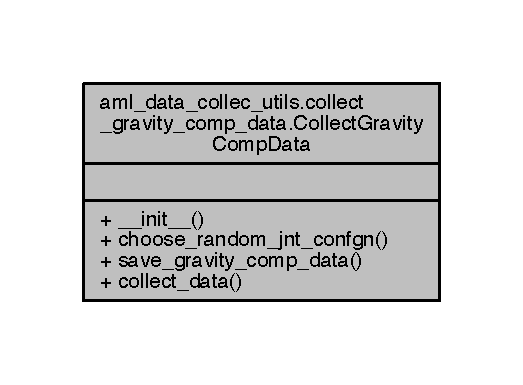
\includegraphics[width=251pt]{classaml__data__collec__utils_1_1collect__gravity__comp__data_1_1_collect_gravity_comp_data__coll__graph}
\end{center}
\end{figure}
\subsection*{Public Member Functions}
\begin{DoxyCompactItemize}
\item 
\hypertarget{classaml__data__collec__utils_1_1collect__gravity__comp__data_1_1_collect_gravity_comp_data_aa9326f995b23f38beee734657b7b0463}{}\label{classaml__data__collec__utils_1_1collect__gravity__comp__data_1_1_collect_gravity_comp_data_aa9326f995b23f38beee734657b7b0463} 
def {\bfseries \+\_\+\+\_\+init\+\_\+\+\_\+} (self, robot\+\_\+interface, data\+\_\+cnt=10, sample\+\_\+rate=50)
\item 
\hypertarget{classaml__data__collec__utils_1_1collect__gravity__comp__data_1_1_collect_gravity_comp_data_a94e8e8c3608993caa6e55fcd90c4ecd8}{}\label{classaml__data__collec__utils_1_1collect__gravity__comp__data_1_1_collect_gravity_comp_data_a94e8e8c3608993caa6e55fcd90c4ecd8} 
def {\bfseries choose\+\_\+random\+\_\+jnt\+\_\+confgn} (self)
\item 
\hypertarget{classaml__data__collec__utils_1_1collect__gravity__comp__data_1_1_collect_gravity_comp_data_a3084abc6f389d5930610e9a0a537a6d7}{}\label{classaml__data__collec__utils_1_1collect__gravity__comp__data_1_1_collect_gravity_comp_data_a3084abc6f389d5930610e9a0a537a6d7} 
def {\bfseries save\+\_\+gravity\+\_\+comp\+\_\+data} (self, event)
\item 
\hypertarget{classaml__data__collec__utils_1_1collect__gravity__comp__data_1_1_collect_gravity_comp_data_a841b1dda70c04964297beaee86345013}{}\label{classaml__data__collec__utils_1_1collect__gravity__comp__data_1_1_collect_gravity_comp_data_a841b1dda70c04964297beaee86345013} 
def {\bfseries collect\+\_\+data} (self)
\end{DoxyCompactItemize}


The documentation for this class was generated from the following file\+:\begin{DoxyCompactItemize}
\item 
aml\+\_\+data\+\_\+collec\+\_\+utils/src/aml\+\_\+data\+\_\+collec\+\_\+utils/collect\+\_\+gravity\+\_\+comp\+\_\+data.\+py\end{DoxyCompactItemize}

\hypertarget{structcomm__settings}{\section{comm\-\_\-settings Struct Reference}
\label{structcomm__settings}\index{comm\-\_\-settings@{comm\-\_\-settings}}
}


Collaboration diagram for comm\-\_\-settings\-:
\nopagebreak
\begin{figure}[H]
\begin{center}
\leavevmode
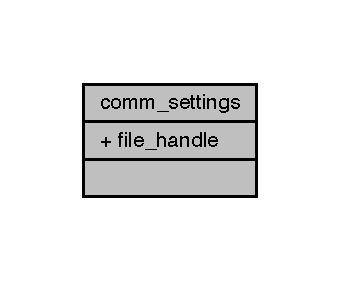
\includegraphics[width=162pt]{structcomm__settings__coll__graph}
\end{center}
\end{figure}
\subsection*{Public Attributes}
\begin{DoxyCompactItemize}
\item 
\hypertarget{structcomm__settings_a337e29e082a3b6b3c5d28634ea09d7fa}{\hyperlink{qbmove__communications_8h_ab521aa5010fb1afb801a899a55569e03}{H\-A\-N\-D\-L\-E} {\bfseries file\-\_\-handle}}\label{structcomm__settings_a337e29e082a3b6b3c5d28634ea09d7fa}

\end{DoxyCompactItemize}


The documentation for this struct was generated from the following file\-:\begin{DoxyCompactItemize}
\item 
aml\-\_\-drivers/aml\-\_\-pisa\-\_\-hand/qb\-A\-P\-I/src/\hyperlink{qbmove__communications_8h}{qbmove\-\_\-communications.\-h}\end{DoxyCompactItemize}

\hypertarget{classaml__ctrl_1_1controller_1_1_controller}{\section{aml\-\_\-ctrl.\-controller.\-Controller Class Reference}
\label{classaml__ctrl_1_1controller_1_1_controller}\index{aml\-\_\-ctrl.\-controller.\-Controller@{aml\-\_\-ctrl.\-controller.\-Controller}}
}


Inheritance diagram for aml\-\_\-ctrl.\-controller.\-Controller\-:
\nopagebreak
\begin{figure}[H]
\begin{center}
\leavevmode
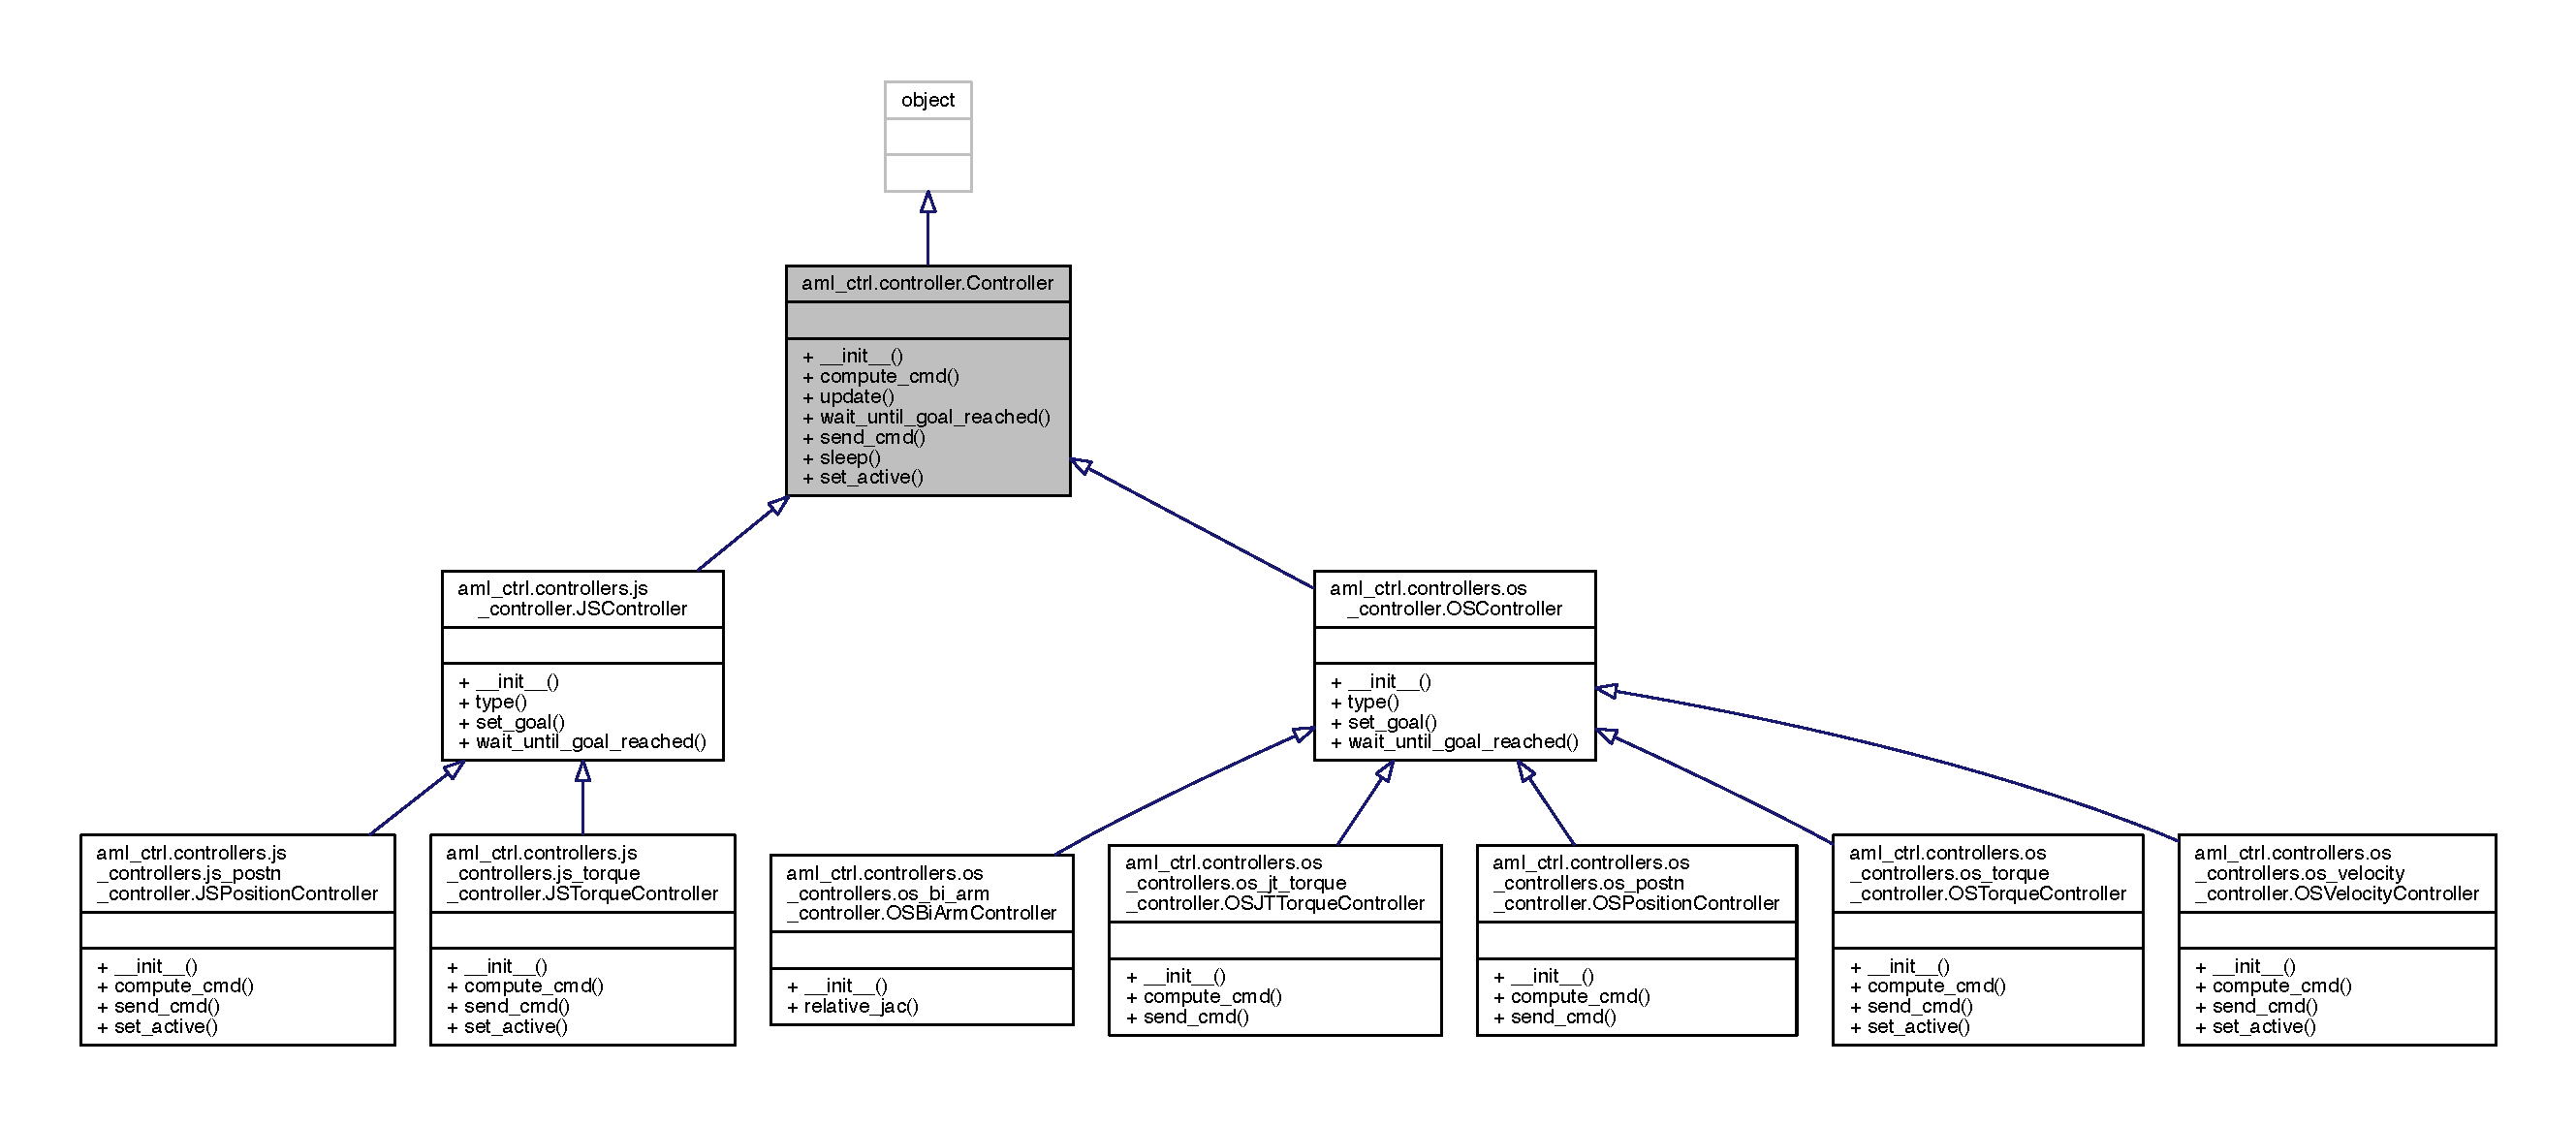
\includegraphics[width=350pt]{classaml__ctrl_1_1controller_1_1_controller__inherit__graph}
\end{center}
\end{figure}


Collaboration diagram for aml\-\_\-ctrl.\-controller.\-Controller\-:
\nopagebreak
\begin{figure}[H]
\begin{center}
\leavevmode
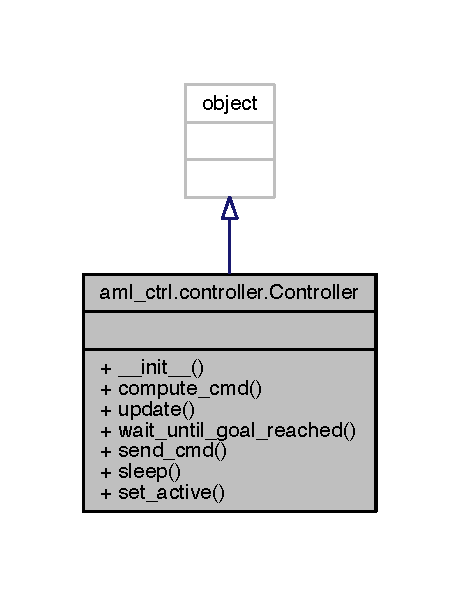
\includegraphics[width=218pt]{classaml__ctrl_1_1controller_1_1_controller__coll__graph}
\end{center}
\end{figure}
\subsection*{Public Member Functions}
\begin{DoxyCompactItemize}
\item 
\hypertarget{classaml__ctrl_1_1controller_1_1_controller_ac1a1888ac43afe5d53e3120d3370db9e}{def {\bfseries \-\_\-\-\_\-init\-\_\-\-\_\-}}\label{classaml__ctrl_1_1controller_1_1_controller_ac1a1888ac43afe5d53e3120d3370db9e}

\item 
\hypertarget{classaml__ctrl_1_1controller_1_1_controller_aace14d69a66dfa391a7d1c8d137b4fe2}{def {\bfseries compute\-\_\-cmd}}\label{classaml__ctrl_1_1controller_1_1_controller_aace14d69a66dfa391a7d1c8d137b4fe2}

\item 
\hypertarget{classaml__ctrl_1_1controller_1_1_controller_ad6f4761cc5211316e70a424472748a2a}{def {\bfseries update}}\label{classaml__ctrl_1_1controller_1_1_controller_ad6f4761cc5211316e70a424472748a2a}

\item 
\hypertarget{classaml__ctrl_1_1controller_1_1_controller_a06f4b5748924ca72a3a6f349370122cd}{def {\bfseries wait\-\_\-until\-\_\-goal\-\_\-reached}}\label{classaml__ctrl_1_1controller_1_1_controller_a06f4b5748924ca72a3a6f349370122cd}

\item 
\hypertarget{classaml__ctrl_1_1controller_1_1_controller_a341e4994f8a876aef85601d622afc968}{def {\bfseries send\-\_\-cmd}}\label{classaml__ctrl_1_1controller_1_1_controller_a341e4994f8a876aef85601d622afc968}

\item 
\hypertarget{classaml__ctrl_1_1controller_1_1_controller_a4047e0ef3a57caf51b599f6d0dc78fe1}{def {\bfseries sleep}}\label{classaml__ctrl_1_1controller_1_1_controller_a4047e0ef3a57caf51b599f6d0dc78fe1}

\item 
\hypertarget{classaml__ctrl_1_1controller_1_1_controller_ab3cf24f3dae223949e893bc61595c89e}{def {\bfseries set\-\_\-active}}\label{classaml__ctrl_1_1controller_1_1_controller_ab3cf24f3dae223949e893bc61595c89e}

\item 
\hypertarget{classaml__ctrl_1_1controller_1_1_controller_a1952a0675d40dee30d917b3f00fe555f}{def {\bfseries is\-\_\-active}}\label{classaml__ctrl_1_1controller_1_1_controller_a1952a0675d40dee30d917b3f00fe555f}

\end{DoxyCompactItemize}


The documentation for this class was generated from the following file\-:\begin{DoxyCompactItemize}
\item 
aml\-\_\-ctrl/src/aml\-\_\-ctrl/controller.\-py\end{DoxyCompactItemize}

\hypertarget{classaml__io_1_1data__manager_1_1_data_manager}{}\section{aml\+\_\+io.\+data\+\_\+manager.\+Data\+Manager Class Reference}
\label{classaml__io_1_1data__manager_1_1_data_manager}\index{aml\+\_\+io.\+data\+\_\+manager.\+Data\+Manager@{aml\+\_\+io.\+data\+\_\+manager.\+Data\+Manager}}


Inheritance diagram for aml\+\_\+io.\+data\+\_\+manager.\+Data\+Manager\+:\nopagebreak
\begin{figure}[H]
\begin{center}
\leavevmode
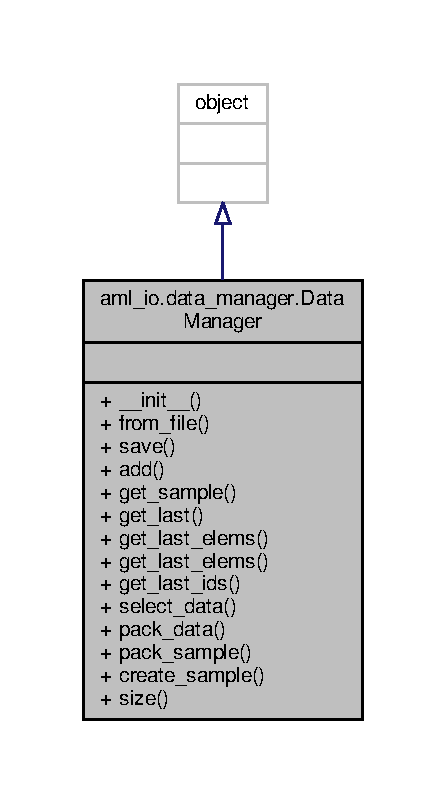
\includegraphics[width=216pt]{classaml__io_1_1data__manager_1_1_data_manager__inherit__graph}
\end{center}
\end{figure}


Collaboration diagram for aml\+\_\+io.\+data\+\_\+manager.\+Data\+Manager\+:\nopagebreak
\begin{figure}[H]
\begin{center}
\leavevmode
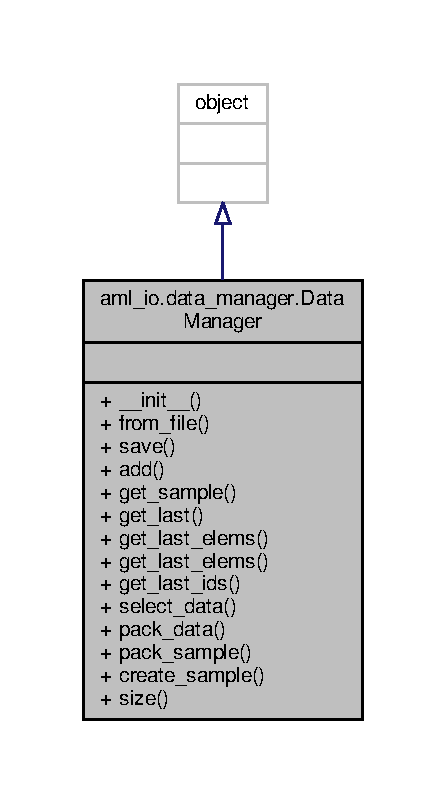
\includegraphics[width=216pt]{classaml__io_1_1data__manager_1_1_data_manager__coll__graph}
\end{center}
\end{figure}
\subsection*{Public Member Functions}
\begin{DoxyCompactItemize}
\item 
\hypertarget{classaml__io_1_1data__manager_1_1_data_manager_a75b042e808d5e6a66c14bf57b56a03fc}{}\label{classaml__io_1_1data__manager_1_1_data_manager_a75b042e808d5e6a66c14bf57b56a03fc} 
def {\bfseries \+\_\+\+\_\+init\+\_\+\+\_\+} (self, data=\mbox{[}$\,$\mbox{]})
\item 
\hypertarget{classaml__io_1_1data__manager_1_1_data_manager_accefddb095ef354e6f4ae639164e08aa}{}\label{classaml__io_1_1data__manager_1_1_data_manager_accefddb095ef354e6f4ae639164e08aa} 
def {\bfseries from\+\_\+file} (cls, filepath, filenames)
\item 
\hypertarget{classaml__io_1_1data__manager_1_1_data_manager_a81de5eeb6512756573939fdf2b45d6c2}{}\label{classaml__io_1_1data__manager_1_1_data_manager_a81de5eeb6512756573939fdf2b45d6c2} 
def {\bfseries save} (self, filename)
\item 
\hypertarget{classaml__io_1_1data__manager_1_1_data_manager_a280fc9cb608f2ea8fc81ebf8f91858e8}{}\label{classaml__io_1_1data__manager_1_1_data_manager_a280fc9cb608f2ea8fc81ebf8f91858e8} 
def {\bfseries add} (self, sample)
\item 
\hypertarget{classaml__io_1_1data__manager_1_1_data_manager_ad816701ca9036e4e265f007a4653171e}{}\label{classaml__io_1_1data__manager_1_1_data_manager_ad816701ca9036e4e265f007a4653171e} 
def {\bfseries get\+\_\+sample} (self, idx, key)
\item 
\hypertarget{classaml__io_1_1data__manager_1_1_data_manager_a74bd27486642541e462ecab78e9a8e24}{}\label{classaml__io_1_1data__manager_1_1_data_manager_a74bd27486642541e462ecab78e9a8e24} 
def {\bfseries get\+\_\+last} (self)
\item 
\hypertarget{classaml__io_1_1data__manager_1_1_data_manager_ad6e5e6cda6ea50e0610b6ccac5d085e2}{}\label{classaml__io_1_1data__manager_1_1_data_manager_ad6e5e6cda6ea50e0610b6ccac5d085e2} 
def {\bfseries get\+\_\+last\+\_\+elems} (self, n=1)
\item 
\hypertarget{classaml__io_1_1data__manager_1_1_data_manager_ad6e5e6cda6ea50e0610b6ccac5d085e2}{}\label{classaml__io_1_1data__manager_1_1_data_manager_ad6e5e6cda6ea50e0610b6ccac5d085e2} 
def {\bfseries get\+\_\+last\+\_\+elems} (self, n=1)
\item 
\hypertarget{classaml__io_1_1data__manager_1_1_data_manager_a01a098a7f0905659c0570de863aabb25}{}\label{classaml__io_1_1data__manager_1_1_data_manager_a01a098a7f0905659c0570de863aabb25} 
def {\bfseries get\+\_\+last\+\_\+ids} (self, n=1)
\item 
\hypertarget{classaml__io_1_1data__manager_1_1_data_manager_aad58f7c69f6c06eb34675010533a8aac}{}\label{classaml__io_1_1data__manager_1_1_data_manager_aad58f7c69f6c06eb34675010533a8aac} 
def {\bfseries select\+\_\+data} (self, ids=None)
\item 
\hypertarget{classaml__io_1_1data__manager_1_1_data_manager_af0c7cf0fcd554d702cf895b33a1a2b5a}{}\label{classaml__io_1_1data__manager_1_1_data_manager_af0c7cf0fcd554d702cf895b33a1a2b5a} 
def {\bfseries pack\+\_\+data} (self, keys, sub\+\_\+keys=None, ids=None)
\item 
\hypertarget{classaml__io_1_1data__manager_1_1_data_manager_a3df42b15ac20a5178f71e420eb2a9241}{}\label{classaml__io_1_1data__manager_1_1_data_manager_a3df42b15ac20a5178f71e420eb2a9241} 
def {\bfseries pack\+\_\+sample} (self, x\+\_\+keys, x\+\_\+sub\+\_\+keys, y\+\_\+keys, y\+\_\+sub\+\_\+keys, ids=None)
\item 
\hypertarget{classaml__io_1_1data__manager_1_1_data_manager_a3cf16fc43ca8af46405c4c9addbc0b0b}{}\label{classaml__io_1_1data__manager_1_1_data_manager_a3cf16fc43ca8af46405c4c9addbc0b0b} 
def {\bfseries create\+\_\+sample} (self)
\item 
\hypertarget{classaml__io_1_1data__manager_1_1_data_manager_a1a4f99ae3887cb1076b39bc747ed3b4d}{}\label{classaml__io_1_1data__manager_1_1_data_manager_a1a4f99ae3887cb1076b39bc747ed3b4d} 
def {\bfseries size} (self)
\end{DoxyCompactItemize}


The documentation for this class was generated from the following file\+:\begin{DoxyCompactItemize}
\item 
aml\+\_\+io/src/aml\+\_\+io/data\+\_\+manager.\+py\end{DoxyCompactItemize}

\hypertarget{classaml__data__collec__utils_1_1core_1_1data__manager_1_1_data_manager}{}\section{aml\+\_\+data\+\_\+collec\+\_\+utils.\+core.\+data\+\_\+manager.\+Data\+Manager Class Reference}
\label{classaml__data__collec__utils_1_1core_1_1data__manager_1_1_data_manager}\index{aml\+\_\+data\+\_\+collec\+\_\+utils.\+core.\+data\+\_\+manager.\+Data\+Manager@{aml\+\_\+data\+\_\+collec\+\_\+utils.\+core.\+data\+\_\+manager.\+Data\+Manager}}


Inheritance diagram for aml\+\_\+data\+\_\+collec\+\_\+utils.\+core.\+data\+\_\+manager.\+Data\+Manager\+:
\nopagebreak
\begin{figure}[H]
\begin{center}
\leavevmode
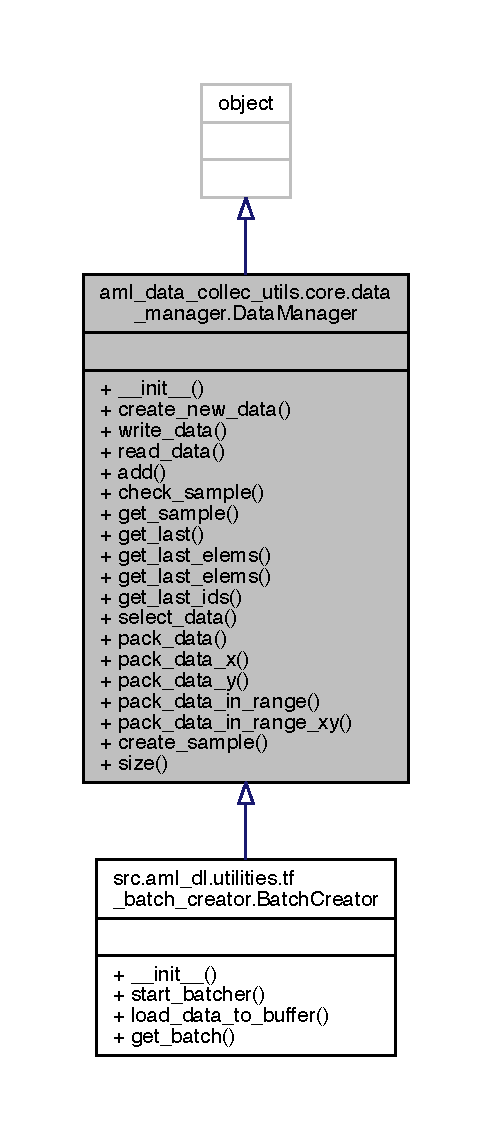
\includegraphics[width=236pt]{classaml__data__collec__utils_1_1core_1_1data__manager_1_1_data_manager__inherit__graph}
\end{center}
\end{figure}


Collaboration diagram for aml\+\_\+data\+\_\+collec\+\_\+utils.\+core.\+data\+\_\+manager.\+Data\+Manager\+:
\nopagebreak
\begin{figure}[H]
\begin{center}
\leavevmode
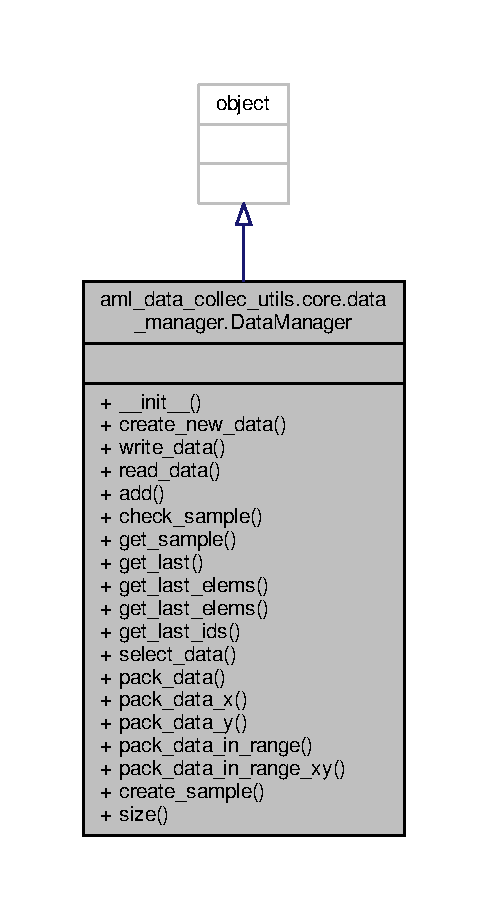
\includegraphics[width=236pt]{classaml__data__collec__utils_1_1core_1_1data__manager_1_1_data_manager__coll__graph}
\end{center}
\end{figure}
\subsection*{Public Member Functions}
\begin{DoxyCompactItemize}
\item 
\hypertarget{classaml__data__collec__utils_1_1core_1_1data__manager_1_1_data_manager_a8d5f6c2f2dd6e9fd067a140cea2a0904}{}\label{classaml__data__collec__utils_1_1core_1_1data__manager_1_1_data_manager_a8d5f6c2f2dd6e9fd067a140cea2a0904} 
def {\bfseries \+\_\+\+\_\+init\+\_\+\+\_\+} (self, append\+\_\+to\+\_\+last\+\_\+file=True, data\+\_\+folder\+\_\+path=None, data\+\_\+name\+\_\+prefix=None, num\+\_\+samples\+\_\+per\+\_\+file=1000)
\item 
\hypertarget{classaml__data__collec__utils_1_1core_1_1data__manager_1_1_data_manager_a00b3fe4436da3dae9419a8064c5ad9ca}{}\label{classaml__data__collec__utils_1_1core_1_1data__manager_1_1_data_manager_a00b3fe4436da3dae9419a8064c5ad9ca} 
def {\bfseries create\+\_\+new\+\_\+data} (self)
\item 
\hypertarget{classaml__data__collec__utils_1_1core_1_1data__manager_1_1_data_manager_a9c7fab4029e1390f60b365facf106769}{}\label{classaml__data__collec__utils_1_1core_1_1data__manager_1_1_data_manager_a9c7fab4029e1390f60b365facf106769} 
def {\bfseries write\+\_\+data} (self)
\item 
\hypertarget{classaml__data__collec__utils_1_1core_1_1data__manager_1_1_data_manager_a9c779a3c3c8f33aa4a7600241189d148}{}\label{classaml__data__collec__utils_1_1core_1_1data__manager_1_1_data_manager_a9c779a3c3c8f33aa4a7600241189d148} 
def {\bfseries read\+\_\+data} (self, data\+\_\+idx)
\item 
\hypertarget{classaml__data__collec__utils_1_1core_1_1data__manager_1_1_data_manager_a4b3e831e21430aee28b787639de33a07}{}\label{classaml__data__collec__utils_1_1core_1_1data__manager_1_1_data_manager_a4b3e831e21430aee28b787639de33a07} 
def {\bfseries add} (self, sample)
\item 
\hypertarget{classaml__data__collec__utils_1_1core_1_1data__manager_1_1_data_manager_a2734742ce00fa78fe05b00d3a51e686f}{}\label{classaml__data__collec__utils_1_1core_1_1data__manager_1_1_data_manager_a2734742ce00fa78fe05b00d3a51e686f} 
def {\bfseries check\+\_\+sample} (self, sample)
\item 
\hypertarget{classaml__data__collec__utils_1_1core_1_1data__manager_1_1_data_manager_ac5d20597c5c48f3da59959be9a4a403f}{}\label{classaml__data__collec__utils_1_1core_1_1data__manager_1_1_data_manager_ac5d20597c5c48f3da59959be9a4a403f} 
def {\bfseries get\+\_\+sample} (self, idx, key)
\item 
\hypertarget{classaml__data__collec__utils_1_1core_1_1data__manager_1_1_data_manager_af4bb596cc3a288f35afdb98db7e372b7}{}\label{classaml__data__collec__utils_1_1core_1_1data__manager_1_1_data_manager_af4bb596cc3a288f35afdb98db7e372b7} 
def {\bfseries get\+\_\+last} (self)
\item 
\hypertarget{classaml__data__collec__utils_1_1core_1_1data__manager_1_1_data_manager_a5cb04122fbd4e9e68e3b58d4d66d1684}{}\label{classaml__data__collec__utils_1_1core_1_1data__manager_1_1_data_manager_a5cb04122fbd4e9e68e3b58d4d66d1684} 
def {\bfseries get\+\_\+last\+\_\+elems} (self, n=1)
\item 
\hypertarget{classaml__data__collec__utils_1_1core_1_1data__manager_1_1_data_manager_a5cb04122fbd4e9e68e3b58d4d66d1684}{}\label{classaml__data__collec__utils_1_1core_1_1data__manager_1_1_data_manager_a5cb04122fbd4e9e68e3b58d4d66d1684} 
def {\bfseries get\+\_\+last\+\_\+elems} (self, n=1)
\item 
\hypertarget{classaml__data__collec__utils_1_1core_1_1data__manager_1_1_data_manager_ac4cc59d510b13daaba59cda32ffd317d}{}\label{classaml__data__collec__utils_1_1core_1_1data__manager_1_1_data_manager_ac4cc59d510b13daaba59cda32ffd317d} 
def {\bfseries get\+\_\+last\+\_\+ids} (self, n=1)
\item 
\hypertarget{classaml__data__collec__utils_1_1core_1_1data__manager_1_1_data_manager_aa6b798ad60ef4414770f03cf5bf87d81}{}\label{classaml__data__collec__utils_1_1core_1_1data__manager_1_1_data_manager_aa6b798ad60ef4414770f03cf5bf87d81} 
def {\bfseries select\+\_\+data} (self, ids=None)
\item 
\hypertarget{classaml__data__collec__utils_1_1core_1_1data__manager_1_1_data_manager_af9f2964c695d4455f5b5151c7530a799}{}\label{classaml__data__collec__utils_1_1core_1_1data__manager_1_1_data_manager_af9f2964c695d4455f5b5151c7530a799} 
def {\bfseries pack\+\_\+data} (self, keys, sub\+\_\+keys=None, ids=None, sample\+\_\+points=None)
\item 
def \hyperlink{classaml__data__collec__utils_1_1core_1_1data__manager_1_1_data_manager_a51ac4a22f0965b1a7e72823bc138a70b}{pack\+\_\+data\+\_\+x} (self, keys, sub\+\_\+keys=None, ids=None, just\+\_\+before=False)
\item 
\hypertarget{classaml__data__collec__utils_1_1core_1_1data__manager_1_1_data_manager_a97caca399fab479e898d03742afe622d}{}\label{classaml__data__collec__utils_1_1core_1_1data__manager_1_1_data_manager_a97caca399fab479e898d03742afe622d} 
def {\bfseries pack\+\_\+data\+\_\+y} (self, keys, sub\+\_\+keys=None, ids=None, just\+\_\+after=False)
\item 
\hypertarget{classaml__data__collec__utils_1_1core_1_1data__manager_1_1_data_manager_ab02da972553d3b3417e72e8888759193}{}\label{classaml__data__collec__utils_1_1core_1_1data__manager_1_1_data_manager_ab02da972553d3b3417e72e8888759193} 
def {\bfseries pack\+\_\+data\+\_\+in\+\_\+range} (self, keys, sub\+\_\+keys=None, ids=None, sample\+\_\+points=None, data\+\_\+file\+\_\+range=None)
\item 
def \hyperlink{classaml__data__collec__utils_1_1core_1_1data__manager_1_1_data_manager_a1afec102117b34b11d170594543439f8}{pack\+\_\+data\+\_\+in\+\_\+range\+\_\+xy} (self, x\+\_\+keys, y\+\_\+keys, x\+\_\+sub\+\_\+keys=None, y\+\_\+sub\+\_\+keys=None, ids=None, before\+\_\+after=False, data\+\_\+file\+\_\+range=None)
\item 
\hypertarget{classaml__data__collec__utils_1_1core_1_1data__manager_1_1_data_manager_a0726ea619d947ce908167ed818de16d3}{}\label{classaml__data__collec__utils_1_1core_1_1data__manager_1_1_data_manager_a0726ea619d947ce908167ed818de16d3} 
def {\bfseries create\+\_\+sample} (self)
\item 
\hypertarget{classaml__data__collec__utils_1_1core_1_1data__manager_1_1_data_manager_adde3cc9ccbf385a50d0dfe610185e417}{}\label{classaml__data__collec__utils_1_1core_1_1data__manager_1_1_data_manager_adde3cc9ccbf385a50d0dfe610185e417} 
def {\bfseries size} (self)
\end{DoxyCompactItemize}


\subsection{Member Function Documentation}
\hypertarget{classaml__data__collec__utils_1_1core_1_1data__manager_1_1_data_manager_a1afec102117b34b11d170594543439f8}{}\label{classaml__data__collec__utils_1_1core_1_1data__manager_1_1_data_manager_a1afec102117b34b11d170594543439f8} 
\index{aml\+\_\+data\+\_\+collec\+\_\+utils\+::core\+::data\+\_\+manager\+::\+Data\+Manager@{aml\+\_\+data\+\_\+collec\+\_\+utils\+::core\+::data\+\_\+manager\+::\+Data\+Manager}!pack\+\_\+data\+\_\+in\+\_\+range\+\_\+xy@{pack\+\_\+data\+\_\+in\+\_\+range\+\_\+xy}}
\index{pack\+\_\+data\+\_\+in\+\_\+range\+\_\+xy@{pack\+\_\+data\+\_\+in\+\_\+range\+\_\+xy}!aml\+\_\+data\+\_\+collec\+\_\+utils\+::core\+::data\+\_\+manager\+::\+Data\+Manager@{aml\+\_\+data\+\_\+collec\+\_\+utils\+::core\+::data\+\_\+manager\+::\+Data\+Manager}}
\subsubsection{\texorpdfstring{pack\+\_\+data\+\_\+in\+\_\+range\+\_\+xy()}{pack\_data\_in\_range\_xy()}}
{\footnotesize\ttfamily def aml\+\_\+data\+\_\+collec\+\_\+utils.\+core.\+data\+\_\+manager.\+Data\+Manager.\+pack\+\_\+data\+\_\+in\+\_\+range\+\_\+xy (\begin{DoxyParamCaption}\item[{}]{self,  }\item[{}]{x\+\_\+keys,  }\item[{}]{y\+\_\+keys,  }\item[{}]{x\+\_\+sub\+\_\+keys = {\ttfamily None},  }\item[{}]{y\+\_\+sub\+\_\+keys = {\ttfamily None},  }\item[{}]{ids = {\ttfamily None},  }\item[{}]{before\+\_\+after = {\ttfamily False},  }\item[{}]{data\+\_\+file\+\_\+range = {\ttfamily None} }\end{DoxyParamCaption})}

\begin{DoxyVerb}This function is for getting a specific set of files from the hard disk
data_file_range reads the given number of files from the hard disk
if data_file_range argument is false, it will just read the penultimate file.
ids chooses the data ids within a sample contained in a datafile, usually there are 5 samples per data file
before_after argument if set true would read only first point in a sample and the last point in a sample
\end{DoxyVerb}
 \hypertarget{classaml__data__collec__utils_1_1core_1_1data__manager_1_1_data_manager_a51ac4a22f0965b1a7e72823bc138a70b}{}\label{classaml__data__collec__utils_1_1core_1_1data__manager_1_1_data_manager_a51ac4a22f0965b1a7e72823bc138a70b} 
\index{aml\+\_\+data\+\_\+collec\+\_\+utils\+::core\+::data\+\_\+manager\+::\+Data\+Manager@{aml\+\_\+data\+\_\+collec\+\_\+utils\+::core\+::data\+\_\+manager\+::\+Data\+Manager}!pack\+\_\+data\+\_\+x@{pack\+\_\+data\+\_\+x}}
\index{pack\+\_\+data\+\_\+x@{pack\+\_\+data\+\_\+x}!aml\+\_\+data\+\_\+collec\+\_\+utils\+::core\+::data\+\_\+manager\+::\+Data\+Manager@{aml\+\_\+data\+\_\+collec\+\_\+utils\+::core\+::data\+\_\+manager\+::\+Data\+Manager}}
\subsubsection{\texorpdfstring{pack\+\_\+data\+\_\+x()}{pack\_data\_x()}}
{\footnotesize\ttfamily def aml\+\_\+data\+\_\+collec\+\_\+utils.\+core.\+data\+\_\+manager.\+Data\+Manager.\+pack\+\_\+data\+\_\+x (\begin{DoxyParamCaption}\item[{}]{self,  }\item[{}]{keys,  }\item[{}]{sub\+\_\+keys = {\ttfamily None},  }\item[{}]{ids = {\ttfamily None},  }\item[{}]{just\+\_\+before = {\ttfamily False} }\end{DoxyParamCaption})}

\begin{DoxyVerb}just_before argument is to be passed if only the starting data point is required.
fundamentally this is a redundant function!
\end{DoxyVerb}
 

The documentation for this class was generated from the following file\+:\begin{DoxyCompactItemize}
\item 
aml\+\_\+data\+\_\+collec\+\_\+utils/src/aml\+\_\+data\+\_\+collec\+\_\+utils/core/data\+\_\+manager.\+py\end{DoxyCompactItemize}

\hypertarget{classaml__data__collec__utils_1_1record__sample_1_1_data_manager}{\section{aml\-\_\-data\-\_\-collec\-\_\-utils.\-record\-\_\-sample.\-Data\-Manager Class Reference}
\label{classaml__data__collec__utils_1_1record__sample_1_1_data_manager}\index{aml\-\_\-data\-\_\-collec\-\_\-utils.\-record\-\_\-sample.\-Data\-Manager@{aml\-\_\-data\-\_\-collec\-\_\-utils.\-record\-\_\-sample.\-Data\-Manager}}
}


Collaboration diagram for aml\-\_\-data\-\_\-collec\-\_\-utils.\-record\-\_\-sample.\-Data\-Manager\-:\nopagebreak
\begin{figure}[H]
\begin{center}
\leavevmode
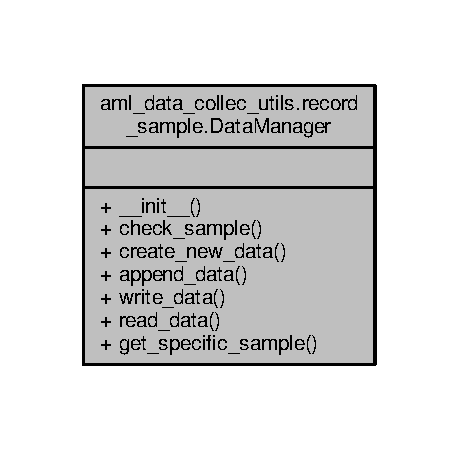
\includegraphics[width=220pt]{classaml__data__collec__utils_1_1record__sample_1_1_data_manager__coll__graph}
\end{center}
\end{figure}
\subsection*{Public Member Functions}
\begin{DoxyCompactItemize}
\item 
\hypertarget{classaml__data__collec__utils_1_1record__sample_1_1_data_manager_a966eab202c69988ff7ae109043cda6a9}{def {\bfseries \-\_\-\-\_\-init\-\_\-\-\_\-}}\label{classaml__data__collec__utils_1_1record__sample_1_1_data_manager_a966eab202c69988ff7ae109043cda6a9}

\item 
\hypertarget{classaml__data__collec__utils_1_1record__sample_1_1_data_manager_a1635586a623f54e627cbc38a6500e67b}{def {\bfseries check\-\_\-sample}}\label{classaml__data__collec__utils_1_1record__sample_1_1_data_manager_a1635586a623f54e627cbc38a6500e67b}

\item 
\hypertarget{classaml__data__collec__utils_1_1record__sample_1_1_data_manager_a409f6d441ea5b00171f42a04c2b64e93}{def {\bfseries create\-\_\-new\-\_\-data}}\label{classaml__data__collec__utils_1_1record__sample_1_1_data_manager_a409f6d441ea5b00171f42a04c2b64e93}

\item 
\hypertarget{classaml__data__collec__utils_1_1record__sample_1_1_data_manager_a6fbb84e06370cee2957c36a6182e4e91}{def {\bfseries append\-\_\-data}}\label{classaml__data__collec__utils_1_1record__sample_1_1_data_manager_a6fbb84e06370cee2957c36a6182e4e91}

\item 
\hypertarget{classaml__data__collec__utils_1_1record__sample_1_1_data_manager_ab46c74dad620a5484a08b88918c2c6aa}{def {\bfseries write\-\_\-data}}\label{classaml__data__collec__utils_1_1record__sample_1_1_data_manager_ab46c74dad620a5484a08b88918c2c6aa}

\item 
\hypertarget{classaml__data__collec__utils_1_1record__sample_1_1_data_manager_a7724d8a3d3df1b3c5a87620e005b5f96}{def {\bfseries read\-\_\-data}}\label{classaml__data__collec__utils_1_1record__sample_1_1_data_manager_a7724d8a3d3df1b3c5a87620e005b5f96}

\item 
\hypertarget{classaml__data__collec__utils_1_1record__sample_1_1_data_manager_a5770a65124b6e2c1e0f94fd2237e8d2d}{def {\bfseries get\-\_\-specific\-\_\-sample}}\label{classaml__data__collec__utils_1_1record__sample_1_1_data_manager_a5770a65124b6e2c1e0f94fd2237e8d2d}

\end{DoxyCompactItemize}


The documentation for this class was generated from the following file\-:\begin{DoxyCompactItemize}
\item 
aml\-\_\-data\-\_\-collec\-\_\-utils/src/aml\-\_\-data\-\_\-collec\-\_\-utils/record\-\_\-sample.\-py\end{DoxyCompactItemize}

\hypertarget{classaml__robot_1_1box2d_1_1data__manager_1_1_data_manager}{}\section{aml\+\_\+robot.\+box2d.\+data\+\_\+manager.\+Data\+Manager Class Reference}
\label{classaml__robot_1_1box2d_1_1data__manager_1_1_data_manager}\index{aml\+\_\+robot.\+box2d.\+data\+\_\+manager.\+Data\+Manager@{aml\+\_\+robot.\+box2d.\+data\+\_\+manager.\+Data\+Manager}}


Inheritance diagram for aml\+\_\+robot.\+box2d.\+data\+\_\+manager.\+Data\+Manager\+:\nopagebreak
\begin{figure}[H]
\begin{center}
\leavevmode
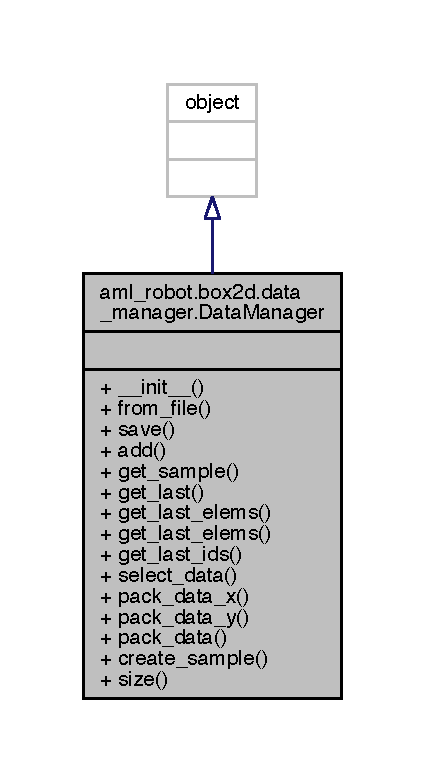
\includegraphics[width=204pt]{classaml__robot_1_1box2d_1_1data__manager_1_1_data_manager__inherit__graph}
\end{center}
\end{figure}


Collaboration diagram for aml\+\_\+robot.\+box2d.\+data\+\_\+manager.\+Data\+Manager\+:\nopagebreak
\begin{figure}[H]
\begin{center}
\leavevmode
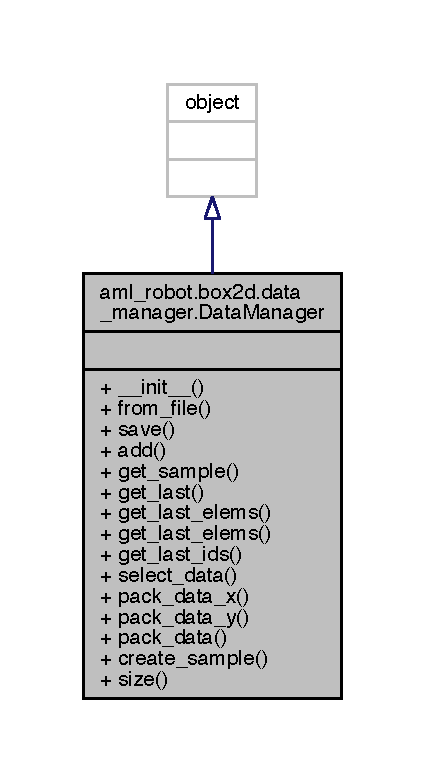
\includegraphics[width=204pt]{classaml__robot_1_1box2d_1_1data__manager_1_1_data_manager__coll__graph}
\end{center}
\end{figure}
\subsection*{Public Member Functions}
\begin{DoxyCompactItemize}
\item 
\hypertarget{classaml__robot_1_1box2d_1_1data__manager_1_1_data_manager_aa0580187539e82c3ceac6917bffe62fa}{}\label{classaml__robot_1_1box2d_1_1data__manager_1_1_data_manager_aa0580187539e82c3ceac6917bffe62fa} 
def {\bfseries \+\_\+\+\_\+init\+\_\+\+\_\+} (self, data=\mbox{[}$\,$\mbox{]})
\item 
\hypertarget{classaml__robot_1_1box2d_1_1data__manager_1_1_data_manager_a400cf525806b262ec07a4432886ce611}{}\label{classaml__robot_1_1box2d_1_1data__manager_1_1_data_manager_a400cf525806b262ec07a4432886ce611} 
def {\bfseries from\+\_\+file} (cls, filename)
\item 
\hypertarget{classaml__robot_1_1box2d_1_1data__manager_1_1_data_manager_a1d5d0230feeab6bd931b3fcebbf7f5f8}{}\label{classaml__robot_1_1box2d_1_1data__manager_1_1_data_manager_a1d5d0230feeab6bd931b3fcebbf7f5f8} 
def {\bfseries save} (self, filename)
\item 
\hypertarget{classaml__robot_1_1box2d_1_1data__manager_1_1_data_manager_a00530313dc94c0c8dd2da7eb50d3739e}{}\label{classaml__robot_1_1box2d_1_1data__manager_1_1_data_manager_a00530313dc94c0c8dd2da7eb50d3739e} 
def {\bfseries add} (self, sample)
\item 
\hypertarget{classaml__robot_1_1box2d_1_1data__manager_1_1_data_manager_a2ccfb6f0938fccc05d6c44670d62e82e}{}\label{classaml__robot_1_1box2d_1_1data__manager_1_1_data_manager_a2ccfb6f0938fccc05d6c44670d62e82e} 
def {\bfseries get\+\_\+sample} (self, idx, key)
\item 
\hypertarget{classaml__robot_1_1box2d_1_1data__manager_1_1_data_manager_a65e78ddd432d63b011c9daffa16270fb}{}\label{classaml__robot_1_1box2d_1_1data__manager_1_1_data_manager_a65e78ddd432d63b011c9daffa16270fb} 
def {\bfseries get\+\_\+last} (self)
\item 
\hypertarget{classaml__robot_1_1box2d_1_1data__manager_1_1_data_manager_a229d07bd1289ae076b6d85006fb79317}{}\label{classaml__robot_1_1box2d_1_1data__manager_1_1_data_manager_a229d07bd1289ae076b6d85006fb79317} 
def {\bfseries get\+\_\+last\+\_\+elems} (self, n=1)
\item 
\hypertarget{classaml__robot_1_1box2d_1_1data__manager_1_1_data_manager_a229d07bd1289ae076b6d85006fb79317}{}\label{classaml__robot_1_1box2d_1_1data__manager_1_1_data_manager_a229d07bd1289ae076b6d85006fb79317} 
def {\bfseries get\+\_\+last\+\_\+elems} (self, n=1)
\item 
\hypertarget{classaml__robot_1_1box2d_1_1data__manager_1_1_data_manager_a4f5a35574b483916068562d4d9f9c19c}{}\label{classaml__robot_1_1box2d_1_1data__manager_1_1_data_manager_a4f5a35574b483916068562d4d9f9c19c} 
def {\bfseries get\+\_\+last\+\_\+ids} (self, n=1)
\item 
\hypertarget{classaml__robot_1_1box2d_1_1data__manager_1_1_data_manager_aa573ee39665d43261bb768c1c3c1cb64}{}\label{classaml__robot_1_1box2d_1_1data__manager_1_1_data_manager_aa573ee39665d43261bb768c1c3c1cb64} 
def {\bfseries select\+\_\+data} (self, ids=None)
\item 
\hypertarget{classaml__robot_1_1box2d_1_1data__manager_1_1_data_manager_a3351b75171e381a07c89fabb723c770b}{}\label{classaml__robot_1_1box2d_1_1data__manager_1_1_data_manager_a3351b75171e381a07c89fabb723c770b} 
def {\bfseries pack\+\_\+data\+\_\+x} (self, keys, ids=None)
\item 
\hypertarget{classaml__robot_1_1box2d_1_1data__manager_1_1_data_manager_a73f284159c9b215bf6884565caf0f601}{}\label{classaml__robot_1_1box2d_1_1data__manager_1_1_data_manager_a73f284159c9b215bf6884565caf0f601} 
def {\bfseries pack\+\_\+data\+\_\+y} (self, ids=None)
\item 
\hypertarget{classaml__robot_1_1box2d_1_1data__manager_1_1_data_manager_ad9975a5ada92b83489e2ccd80db88f13}{}\label{classaml__robot_1_1box2d_1_1data__manager_1_1_data_manager_ad9975a5ada92b83489e2ccd80db88f13} 
def {\bfseries pack\+\_\+data} (self, keys, ids=None)
\item 
\hypertarget{classaml__robot_1_1box2d_1_1data__manager_1_1_data_manager_a4146de256982fba71b91a46a9117ae60}{}\label{classaml__robot_1_1box2d_1_1data__manager_1_1_data_manager_a4146de256982fba71b91a46a9117ae60} 
def {\bfseries create\+\_\+sample} (self)
\item 
\hypertarget{classaml__robot_1_1box2d_1_1data__manager_1_1_data_manager_aaa5cac201a4804c05c4ad9ee950aca33}{}\label{classaml__robot_1_1box2d_1_1data__manager_1_1_data_manager_aaa5cac201a4804c05c4ad9ee950aca33} 
def {\bfseries size} (self)
\end{DoxyCompactItemize}


The documentation for this class was generated from the following file\+:\begin{DoxyCompactItemize}
\item 
aml\+\_\+robot/src/aml\+\_\+robot/box2d/data\+\_\+manager.\+py\end{DoxyCompactItemize}

\hypertarget{classaml__data__collec__utils_1_1core_1_1data__recorder_1_1_data_recorder}{\section{aml\-\_\-data\-\_\-collec\-\_\-utils.\-core.\-data\-\_\-recorder.\-Data\-Recorder Class Reference}
\label{classaml__data__collec__utils_1_1core_1_1data__recorder_1_1_data_recorder}\index{aml\-\_\-data\-\_\-collec\-\_\-utils.\-core.\-data\-\_\-recorder.\-Data\-Recorder@{aml\-\_\-data\-\_\-collec\-\_\-utils.\-core.\-data\-\_\-recorder.\-Data\-Recorder}}
}


Inheritance diagram for aml\-\_\-data\-\_\-collec\-\_\-utils.\-core.\-data\-\_\-recorder.\-Data\-Recorder\-:\nopagebreak
\begin{figure}[H]
\begin{center}
\leavevmode
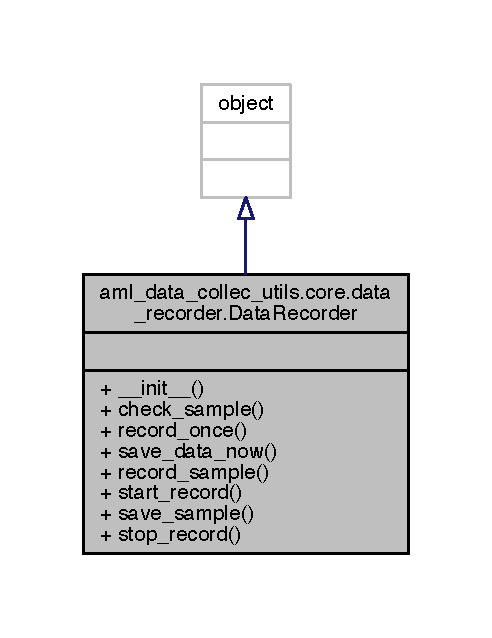
\includegraphics[width=234pt]{classaml__data__collec__utils_1_1core_1_1data__recorder_1_1_data_recorder__inherit__graph}
\end{center}
\end{figure}


Collaboration diagram for aml\-\_\-data\-\_\-collec\-\_\-utils.\-core.\-data\-\_\-recorder.\-Data\-Recorder\-:\nopagebreak
\begin{figure}[H]
\begin{center}
\leavevmode
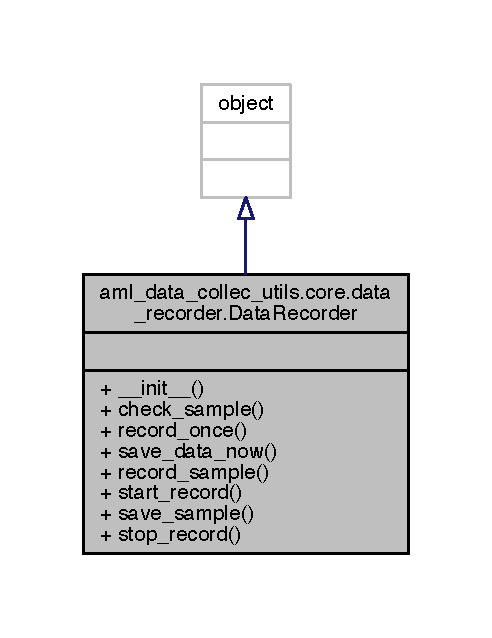
\includegraphics[width=234pt]{classaml__data__collec__utils_1_1core_1_1data__recorder_1_1_data_recorder__coll__graph}
\end{center}
\end{figure}
\subsection*{Public Member Functions}
\begin{DoxyCompactItemize}
\item 
\hypertarget{classaml__data__collec__utils_1_1core_1_1data__recorder_1_1_data_recorder_af30fc89a11eb8f23797d2bc65986e02f}{def {\bfseries \-\_\-\-\_\-init\-\_\-\-\_\-}}\label{classaml__data__collec__utils_1_1core_1_1data__recorder_1_1_data_recorder_af30fc89a11eb8f23797d2bc65986e02f}

\item 
\hypertarget{classaml__data__collec__utils_1_1core_1_1data__recorder_1_1_data_recorder_ac8c97876fbc9ba1f5d386425692350f8}{def {\bfseries check\-\_\-sample}}\label{classaml__data__collec__utils_1_1core_1_1data__recorder_1_1_data_recorder_ac8c97876fbc9ba1f5d386425692350f8}

\item 
\hypertarget{classaml__data__collec__utils_1_1core_1_1data__recorder_1_1_data_recorder_a0657028709128be59ca90df23e9a1a9d}{def {\bfseries record\-\_\-once}}\label{classaml__data__collec__utils_1_1core_1_1data__recorder_1_1_data_recorder_a0657028709128be59ca90df23e9a1a9d}

\item 
\hypertarget{classaml__data__collec__utils_1_1core_1_1data__recorder_1_1_data_recorder_a2f2398422b0f75510801188164971882}{def {\bfseries save\-\_\-data\-\_\-now}}\label{classaml__data__collec__utils_1_1core_1_1data__recorder_1_1_data_recorder_a2f2398422b0f75510801188164971882}

\item 
\hypertarget{classaml__data__collec__utils_1_1core_1_1data__recorder_1_1_data_recorder_a40ed019eb5117361ecfb769528a72968}{def {\bfseries record\-\_\-sample}}\label{classaml__data__collec__utils_1_1core_1_1data__recorder_1_1_data_recorder_a40ed019eb5117361ecfb769528a72968}

\item 
\hypertarget{classaml__data__collec__utils_1_1core_1_1data__recorder_1_1_data_recorder_acc481956358b64a8038370f5a8fc9f49}{def {\bfseries start\-\_\-record}}\label{classaml__data__collec__utils_1_1core_1_1data__recorder_1_1_data_recorder_acc481956358b64a8038370f5a8fc9f49}

\item 
\hypertarget{classaml__data__collec__utils_1_1core_1_1data__recorder_1_1_data_recorder_a4bf0d2565d7bf39b7bdd3acc08dd1057}{def {\bfseries save\-\_\-sample}}\label{classaml__data__collec__utils_1_1core_1_1data__recorder_1_1_data_recorder_a4bf0d2565d7bf39b7bdd3acc08dd1057}

\item 
\hypertarget{classaml__data__collec__utils_1_1core_1_1data__recorder_1_1_data_recorder_ad56cbcc53fc7fee273c87e627b3d3f8c}{def {\bfseries stop\-\_\-record}}\label{classaml__data__collec__utils_1_1core_1_1data__recorder_1_1_data_recorder_ad56cbcc53fc7fee273c87e627b3d3f8c}

\end{DoxyCompactItemize}


The documentation for this class was generated from the following file\-:\begin{DoxyCompactItemize}
\item 
aml\-\_\-data\-\_\-collec\-\_\-utils/src/aml\-\_\-data\-\_\-collec\-\_\-utils/core/data\-\_\-recorder.\-py\end{DoxyCompactItemize}

\hypertarget{classaml__lfd_1_1ilqr_1_1ilqr__traj__follow_1_1_d_d_p___traj_follow_class}{\section{aml\-\_\-lfd.\-ilqr.\-ilqr\-\_\-traj\-\_\-follow.\-D\-D\-P\-\_\-\-Traj\-Follow\-Class Class Reference}
\label{classaml__lfd_1_1ilqr_1_1ilqr__traj__follow_1_1_d_d_p___traj_follow_class}\index{aml\-\_\-lfd.\-ilqr.\-ilqr\-\_\-traj\-\_\-follow.\-D\-D\-P\-\_\-\-Traj\-Follow\-Class@{aml\-\_\-lfd.\-ilqr.\-ilqr\-\_\-traj\-\_\-follow.\-D\-D\-P\-\_\-\-Traj\-Follow\-Class}}
}


Collaboration diagram for aml\-\_\-lfd.\-ilqr.\-ilqr\-\_\-traj\-\_\-follow.\-D\-D\-P\-\_\-\-Traj\-Follow\-Class\-:\nopagebreak
\begin{figure}[H]
\begin{center}
\leavevmode
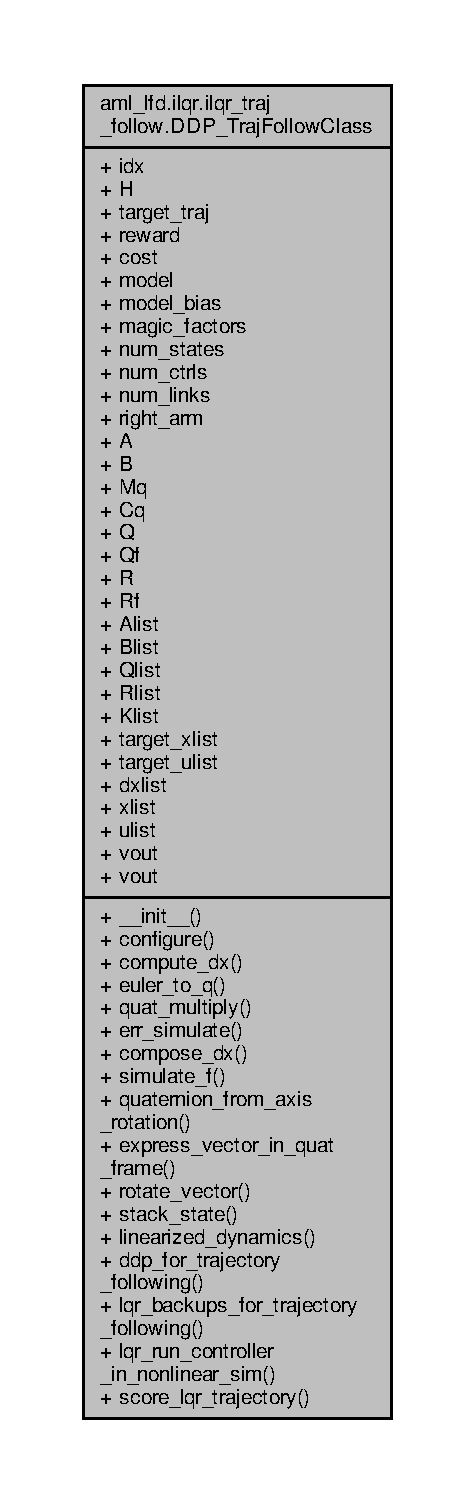
\includegraphics[height=550pt]{classaml__lfd_1_1ilqr_1_1ilqr__traj__follow_1_1_d_d_p___traj_follow_class__coll__graph}
\end{center}
\end{figure}
\subsection*{Public Member Functions}
\begin{DoxyCompactItemize}
\item 
\hypertarget{classaml__lfd_1_1ilqr_1_1ilqr__traj__follow_1_1_d_d_p___traj_follow_class_ad7fc5b47422623c1369ef622a30ba654}{def {\bfseries \-\_\-\-\_\-init\-\_\-\-\_\-}}\label{classaml__lfd_1_1ilqr_1_1ilqr__traj__follow_1_1_d_d_p___traj_follow_class_ad7fc5b47422623c1369ef622a30ba654}

\item 
\hypertarget{classaml__lfd_1_1ilqr_1_1ilqr__traj__follow_1_1_d_d_p___traj_follow_class_ac3673e1d7138eade9bcc0e12e8546322}{def {\bfseries configure}}\label{classaml__lfd_1_1ilqr_1_1ilqr__traj__follow_1_1_d_d_p___traj_follow_class_ac3673e1d7138eade9bcc0e12e8546322}

\item 
\hypertarget{classaml__lfd_1_1ilqr_1_1ilqr__traj__follow_1_1_d_d_p___traj_follow_class_aed985f043586a1740a0181d331f53176}{def {\bfseries compute\-\_\-dx}}\label{classaml__lfd_1_1ilqr_1_1ilqr__traj__follow_1_1_d_d_p___traj_follow_class_aed985f043586a1740a0181d331f53176}

\item 
\hypertarget{classaml__lfd_1_1ilqr_1_1ilqr__traj__follow_1_1_d_d_p___traj_follow_class_ad2e783809690f057364e87eaa52f48ab}{def {\bfseries euler\-\_\-to\-\_\-q}}\label{classaml__lfd_1_1ilqr_1_1ilqr__traj__follow_1_1_d_d_p___traj_follow_class_ad2e783809690f057364e87eaa52f48ab}

\item 
\hypertarget{classaml__lfd_1_1ilqr_1_1ilqr__traj__follow_1_1_d_d_p___traj_follow_class_a33165af92cd027dea290adda63a6b036}{def {\bfseries quat\-\_\-multiply}}\label{classaml__lfd_1_1ilqr_1_1ilqr__traj__follow_1_1_d_d_p___traj_follow_class_a33165af92cd027dea290adda63a6b036}

\item 
\hypertarget{classaml__lfd_1_1ilqr_1_1ilqr__traj__follow_1_1_d_d_p___traj_follow_class_a7f873bf434749da8e00780f991dd875a}{def {\bfseries err\-\_\-simulate}}\label{classaml__lfd_1_1ilqr_1_1ilqr__traj__follow_1_1_d_d_p___traj_follow_class_a7f873bf434749da8e00780f991dd875a}

\item 
\hypertarget{classaml__lfd_1_1ilqr_1_1ilqr__traj__follow_1_1_d_d_p___traj_follow_class_afc28b6ddc1d262b1d5e11312e880db30}{def {\bfseries compose\-\_\-dx}}\label{classaml__lfd_1_1ilqr_1_1ilqr__traj__follow_1_1_d_d_p___traj_follow_class_afc28b6ddc1d262b1d5e11312e880db30}

\item 
\hypertarget{classaml__lfd_1_1ilqr_1_1ilqr__traj__follow_1_1_d_d_p___traj_follow_class_ac0d8f0c54d196a70822308a3b3a3150f}{def {\bfseries simulate\-\_\-f}}\label{classaml__lfd_1_1ilqr_1_1ilqr__traj__follow_1_1_d_d_p___traj_follow_class_ac0d8f0c54d196a70822308a3b3a3150f}

\item 
\hypertarget{classaml__lfd_1_1ilqr_1_1ilqr__traj__follow_1_1_d_d_p___traj_follow_class_abd87fb33b984bf16a7b8a22e156ad9bd}{def {\bfseries quaternion\-\_\-from\-\_\-axis\-\_\-rotation}}\label{classaml__lfd_1_1ilqr_1_1ilqr__traj__follow_1_1_d_d_p___traj_follow_class_abd87fb33b984bf16a7b8a22e156ad9bd}

\item 
\hypertarget{classaml__lfd_1_1ilqr_1_1ilqr__traj__follow_1_1_d_d_p___traj_follow_class_ace91aea7502ef0c2923f74b16e6c5e11}{def {\bfseries express\-\_\-vector\-\_\-in\-\_\-quat\-\_\-frame}}\label{classaml__lfd_1_1ilqr_1_1ilqr__traj__follow_1_1_d_d_p___traj_follow_class_ace91aea7502ef0c2923f74b16e6c5e11}

\item 
\hypertarget{classaml__lfd_1_1ilqr_1_1ilqr__traj__follow_1_1_d_d_p___traj_follow_class_af6bb5e31fe445276d683d947a444d557}{def {\bfseries rotate\-\_\-vector}}\label{classaml__lfd_1_1ilqr_1_1ilqr__traj__follow_1_1_d_d_p___traj_follow_class_af6bb5e31fe445276d683d947a444d557}

\item 
\hypertarget{classaml__lfd_1_1ilqr_1_1ilqr__traj__follow_1_1_d_d_p___traj_follow_class_ae591b82eb361d4c870535bfe9cd3511e}{def {\bfseries stack\-\_\-state}}\label{classaml__lfd_1_1ilqr_1_1ilqr__traj__follow_1_1_d_d_p___traj_follow_class_ae591b82eb361d4c870535bfe9cd3511e}

\item 
\hypertarget{classaml__lfd_1_1ilqr_1_1ilqr__traj__follow_1_1_d_d_p___traj_follow_class_a0c9aed35c760850a40dce2504a8102fc}{def {\bfseries linearized\-\_\-dynamics}}\label{classaml__lfd_1_1ilqr_1_1ilqr__traj__follow_1_1_d_d_p___traj_follow_class_a0c9aed35c760850a40dce2504a8102fc}

\item 
\hypertarget{classaml__lfd_1_1ilqr_1_1ilqr__traj__follow_1_1_d_d_p___traj_follow_class_ad0160a37cf1558a94e5fe280ef363b0f}{def {\bfseries ddp\-\_\-for\-\_\-trajectory\-\_\-following}}\label{classaml__lfd_1_1ilqr_1_1ilqr__traj__follow_1_1_d_d_p___traj_follow_class_ad0160a37cf1558a94e5fe280ef363b0f}

\item 
\hypertarget{classaml__lfd_1_1ilqr_1_1ilqr__traj__follow_1_1_d_d_p___traj_follow_class_a26cfeaef8f2b3c3772e90eafd5550dd2}{def {\bfseries lqr\-\_\-backups\-\_\-for\-\_\-trajectory\-\_\-following}}\label{classaml__lfd_1_1ilqr_1_1ilqr__traj__follow_1_1_d_d_p___traj_follow_class_a26cfeaef8f2b3c3772e90eafd5550dd2}

\item 
\hypertarget{classaml__lfd_1_1ilqr_1_1ilqr__traj__follow_1_1_d_d_p___traj_follow_class_aaf416ec526fdccbbd0b19a57e9372d77}{def {\bfseries lqr\-\_\-run\-\_\-controller\-\_\-in\-\_\-nonlinear\-\_\-sim}}\label{classaml__lfd_1_1ilqr_1_1ilqr__traj__follow_1_1_d_d_p___traj_follow_class_aaf416ec526fdccbbd0b19a57e9372d77}

\item 
\hypertarget{classaml__lfd_1_1ilqr_1_1ilqr__traj__follow_1_1_d_d_p___traj_follow_class_a9459c23b6439beaeb095011e013d3c09}{def {\bfseries score\-\_\-lqr\-\_\-trajectory}}\label{classaml__lfd_1_1ilqr_1_1ilqr__traj__follow_1_1_d_d_p___traj_follow_class_a9459c23b6439beaeb095011e013d3c09}

\end{DoxyCompactItemize}
\subsection*{Public Attributes}
\begin{DoxyCompactItemize}
\item 
\hypertarget{classaml__lfd_1_1ilqr_1_1ilqr__traj__follow_1_1_d_d_p___traj_follow_class_a24d5d726678380440f768704b014d3cb}{{\bfseries idx}}\label{classaml__lfd_1_1ilqr_1_1ilqr__traj__follow_1_1_d_d_p___traj_follow_class_a24d5d726678380440f768704b014d3cb}

\item 
\hypertarget{classaml__lfd_1_1ilqr_1_1ilqr__traj__follow_1_1_d_d_p___traj_follow_class_af293f4032dae063fcef8b87db6f0755d}{{\bfseries H}}\label{classaml__lfd_1_1ilqr_1_1ilqr__traj__follow_1_1_d_d_p___traj_follow_class_af293f4032dae063fcef8b87db6f0755d}

\item 
\hypertarget{classaml__lfd_1_1ilqr_1_1ilqr__traj__follow_1_1_d_d_p___traj_follow_class_afa1787ffdca740b26dea0352871facaa}{{\bfseries target\-\_\-traj}}\label{classaml__lfd_1_1ilqr_1_1ilqr__traj__follow_1_1_d_d_p___traj_follow_class_afa1787ffdca740b26dea0352871facaa}

\item 
\hypertarget{classaml__lfd_1_1ilqr_1_1ilqr__traj__follow_1_1_d_d_p___traj_follow_class_af69890ed626d1d51fd0c0c9c90a07029}{{\bfseries reward}}\label{classaml__lfd_1_1ilqr_1_1ilqr__traj__follow_1_1_d_d_p___traj_follow_class_af69890ed626d1d51fd0c0c9c90a07029}

\item 
\hypertarget{classaml__lfd_1_1ilqr_1_1ilqr__traj__follow_1_1_d_d_p___traj_follow_class_afebda9c04f87f105838bbe8d0d459a9f}{{\bfseries cost}}\label{classaml__lfd_1_1ilqr_1_1ilqr__traj__follow_1_1_d_d_p___traj_follow_class_afebda9c04f87f105838bbe8d0d459a9f}

\item 
\hypertarget{classaml__lfd_1_1ilqr_1_1ilqr__traj__follow_1_1_d_d_p___traj_follow_class_a92ebe7f59db045d57fd0ec0dd5eb8233}{{\bfseries model}}\label{classaml__lfd_1_1ilqr_1_1ilqr__traj__follow_1_1_d_d_p___traj_follow_class_a92ebe7f59db045d57fd0ec0dd5eb8233}

\item 
\hypertarget{classaml__lfd_1_1ilqr_1_1ilqr__traj__follow_1_1_d_d_p___traj_follow_class_a9bbff6812b2bb4ad8498049c36c4456b}{{\bfseries model\-\_\-bias}}\label{classaml__lfd_1_1ilqr_1_1ilqr__traj__follow_1_1_d_d_p___traj_follow_class_a9bbff6812b2bb4ad8498049c36c4456b}

\item 
\hypertarget{classaml__lfd_1_1ilqr_1_1ilqr__traj__follow_1_1_d_d_p___traj_follow_class_a868566fc02ed89a173ed419e4e16f592}{{\bfseries magic\-\_\-factors}}\label{classaml__lfd_1_1ilqr_1_1ilqr__traj__follow_1_1_d_d_p___traj_follow_class_a868566fc02ed89a173ed419e4e16f592}

\item 
\hypertarget{classaml__lfd_1_1ilqr_1_1ilqr__traj__follow_1_1_d_d_p___traj_follow_class_ae474874e12f41dba69615a82c7a8cb60}{{\bfseries num\-\_\-states}}\label{classaml__lfd_1_1ilqr_1_1ilqr__traj__follow_1_1_d_d_p___traj_follow_class_ae474874e12f41dba69615a82c7a8cb60}

\item 
\hypertarget{classaml__lfd_1_1ilqr_1_1ilqr__traj__follow_1_1_d_d_p___traj_follow_class_a9c3bdb7c8a694200ad80c8c1aee526c2}{{\bfseries num\-\_\-ctrls}}\label{classaml__lfd_1_1ilqr_1_1ilqr__traj__follow_1_1_d_d_p___traj_follow_class_a9c3bdb7c8a694200ad80c8c1aee526c2}

\item 
\hypertarget{classaml__lfd_1_1ilqr_1_1ilqr__traj__follow_1_1_d_d_p___traj_follow_class_ab8ccf4574218a1a3e7126f27b3408789}{{\bfseries num\-\_\-links}}\label{classaml__lfd_1_1ilqr_1_1ilqr__traj__follow_1_1_d_d_p___traj_follow_class_ab8ccf4574218a1a3e7126f27b3408789}

\item 
\hypertarget{classaml__lfd_1_1ilqr_1_1ilqr__traj__follow_1_1_d_d_p___traj_follow_class_a50b099d5205a3fa99dbaacd3057cc148}{{\bfseries right\-\_\-arm}}\label{classaml__lfd_1_1ilqr_1_1ilqr__traj__follow_1_1_d_d_p___traj_follow_class_a50b099d5205a3fa99dbaacd3057cc148}

\item 
\hypertarget{classaml__lfd_1_1ilqr_1_1ilqr__traj__follow_1_1_d_d_p___traj_follow_class_ae5267f78b503df5d7ead70bfa2475e97}{{\bfseries A}}\label{classaml__lfd_1_1ilqr_1_1ilqr__traj__follow_1_1_d_d_p___traj_follow_class_ae5267f78b503df5d7ead70bfa2475e97}

\item 
\hypertarget{classaml__lfd_1_1ilqr_1_1ilqr__traj__follow_1_1_d_d_p___traj_follow_class_a785a4e091b777d2b31041be375a46a49}{{\bfseries B}}\label{classaml__lfd_1_1ilqr_1_1ilqr__traj__follow_1_1_d_d_p___traj_follow_class_a785a4e091b777d2b31041be375a46a49}

\item 
\hypertarget{classaml__lfd_1_1ilqr_1_1ilqr__traj__follow_1_1_d_d_p___traj_follow_class_a6d27ee9d34134d8d37f5cf3ebea59741}{{\bfseries Mq}}\label{classaml__lfd_1_1ilqr_1_1ilqr__traj__follow_1_1_d_d_p___traj_follow_class_a6d27ee9d34134d8d37f5cf3ebea59741}

\item 
\hypertarget{classaml__lfd_1_1ilqr_1_1ilqr__traj__follow_1_1_d_d_p___traj_follow_class_ae34c9104cc990dde3a60ac3bad1ca2e3}{{\bfseries Cq}}\label{classaml__lfd_1_1ilqr_1_1ilqr__traj__follow_1_1_d_d_p___traj_follow_class_ae34c9104cc990dde3a60ac3bad1ca2e3}

\item 
\hypertarget{classaml__lfd_1_1ilqr_1_1ilqr__traj__follow_1_1_d_d_p___traj_follow_class_a1d99f2916f1896bd424ba68a1f67e814}{{\bfseries Q}}\label{classaml__lfd_1_1ilqr_1_1ilqr__traj__follow_1_1_d_d_p___traj_follow_class_a1d99f2916f1896bd424ba68a1f67e814}

\item 
\hypertarget{classaml__lfd_1_1ilqr_1_1ilqr__traj__follow_1_1_d_d_p___traj_follow_class_a307ecd9fdbbab36d3bc067730e4fab64}{{\bfseries Qf}}\label{classaml__lfd_1_1ilqr_1_1ilqr__traj__follow_1_1_d_d_p___traj_follow_class_a307ecd9fdbbab36d3bc067730e4fab64}

\item 
\hypertarget{classaml__lfd_1_1ilqr_1_1ilqr__traj__follow_1_1_d_d_p___traj_follow_class_a6f4f259eada3a4e47f5a711747b1e342}{{\bfseries R}}\label{classaml__lfd_1_1ilqr_1_1ilqr__traj__follow_1_1_d_d_p___traj_follow_class_a6f4f259eada3a4e47f5a711747b1e342}

\item 
\hypertarget{classaml__lfd_1_1ilqr_1_1ilqr__traj__follow_1_1_d_d_p___traj_follow_class_abb529fb840b8d7ab8a4207e3f51e29c1}{{\bfseries Rf}}\label{classaml__lfd_1_1ilqr_1_1ilqr__traj__follow_1_1_d_d_p___traj_follow_class_abb529fb840b8d7ab8a4207e3f51e29c1}

\item 
\hypertarget{classaml__lfd_1_1ilqr_1_1ilqr__traj__follow_1_1_d_d_p___traj_follow_class_a61793e7ea328fb11752146fa5106c5e1}{{\bfseries Alist}}\label{classaml__lfd_1_1ilqr_1_1ilqr__traj__follow_1_1_d_d_p___traj_follow_class_a61793e7ea328fb11752146fa5106c5e1}

\item 
\hypertarget{classaml__lfd_1_1ilqr_1_1ilqr__traj__follow_1_1_d_d_p___traj_follow_class_ae5dbe5975a442e1e3f14467cf6d09968}{{\bfseries Blist}}\label{classaml__lfd_1_1ilqr_1_1ilqr__traj__follow_1_1_d_d_p___traj_follow_class_ae5dbe5975a442e1e3f14467cf6d09968}

\item 
\hypertarget{classaml__lfd_1_1ilqr_1_1ilqr__traj__follow_1_1_d_d_p___traj_follow_class_aa003fc26899988835cd9231b709f5e62}{{\bfseries Qlist}}\label{classaml__lfd_1_1ilqr_1_1ilqr__traj__follow_1_1_d_d_p___traj_follow_class_aa003fc26899988835cd9231b709f5e62}

\item 
\hypertarget{classaml__lfd_1_1ilqr_1_1ilqr__traj__follow_1_1_d_d_p___traj_follow_class_a769b8bb1bbd4803d742df4a124930cd0}{{\bfseries Rlist}}\label{classaml__lfd_1_1ilqr_1_1ilqr__traj__follow_1_1_d_d_p___traj_follow_class_a769b8bb1bbd4803d742df4a124930cd0}

\item 
\hypertarget{classaml__lfd_1_1ilqr_1_1ilqr__traj__follow_1_1_d_d_p___traj_follow_class_a9c06e5ea9a384bce048d5c7e3ddc8d93}{{\bfseries Klist}}\label{classaml__lfd_1_1ilqr_1_1ilqr__traj__follow_1_1_d_d_p___traj_follow_class_a9c06e5ea9a384bce048d5c7e3ddc8d93}

\item 
\hypertarget{classaml__lfd_1_1ilqr_1_1ilqr__traj__follow_1_1_d_d_p___traj_follow_class_a100748474b1784ce9203a15edf12cfda}{{\bfseries target\-\_\-xlist}}\label{classaml__lfd_1_1ilqr_1_1ilqr__traj__follow_1_1_d_d_p___traj_follow_class_a100748474b1784ce9203a15edf12cfda}

\item 
\hypertarget{classaml__lfd_1_1ilqr_1_1ilqr__traj__follow_1_1_d_d_p___traj_follow_class_aca8ae4b641b2fb8838e7892de4c55125}{{\bfseries target\-\_\-ulist}}\label{classaml__lfd_1_1ilqr_1_1ilqr__traj__follow_1_1_d_d_p___traj_follow_class_aca8ae4b641b2fb8838e7892de4c55125}

\item 
\hypertarget{classaml__lfd_1_1ilqr_1_1ilqr__traj__follow_1_1_d_d_p___traj_follow_class_a0688bdd96bc836e5de454dc7241d64b8}{{\bfseries dxlist}}\label{classaml__lfd_1_1ilqr_1_1ilqr__traj__follow_1_1_d_d_p___traj_follow_class_a0688bdd96bc836e5de454dc7241d64b8}

\item 
\hypertarget{classaml__lfd_1_1ilqr_1_1ilqr__traj__follow_1_1_d_d_p___traj_follow_class_a203438b84d4591e8cb909e85ed4c8c81}{{\bfseries xlist}}\label{classaml__lfd_1_1ilqr_1_1ilqr__traj__follow_1_1_d_d_p___traj_follow_class_a203438b84d4591e8cb909e85ed4c8c81}

\item 
\hypertarget{classaml__lfd_1_1ilqr_1_1ilqr__traj__follow_1_1_d_d_p___traj_follow_class_a709d529f4e4e60a53ed5119a42ea8605}{{\bfseries ulist}}\label{classaml__lfd_1_1ilqr_1_1ilqr__traj__follow_1_1_d_d_p___traj_follow_class_a709d529f4e4e60a53ed5119a42ea8605}

\end{DoxyCompactItemize}
\subsection*{Static Public Attributes}
\begin{DoxyCompactItemize}
\item 
\hypertarget{classaml__lfd_1_1ilqr_1_1ilqr__traj__follow_1_1_d_d_p___traj_follow_class_a46ee912e03e87a01ae53303079b3bed2}{tuple {\bfseries vout} = self.\-quat\-\_\-multiply( quat\-\_\-multiply ( q, np.\-hstack( np.\-vstack(\mbox{[}0, vin\mbox{]}), np.\-vstack(\mbox{[}q\mbox{[}0\mbox{]},-\/ q\mbox{[}1\-:4\mbox{]}\mbox{]}) ) ) )}\label{classaml__lfd_1_1ilqr_1_1ilqr__traj__follow_1_1_d_d_p___traj_follow_class_a46ee912e03e87a01ae53303079b3bed2}

\item 
\hypertarget{classaml__lfd_1_1ilqr_1_1ilqr__traj__follow_1_1_d_d_p___traj_follow_class_a16c4553ec373478e5f8aae0802a9a198}{list {\bfseries vout} = vout\mbox{[}1\-:4\mbox{]}}\label{classaml__lfd_1_1ilqr_1_1ilqr__traj__follow_1_1_d_d_p___traj_follow_class_a16c4553ec373478e5f8aae0802a9a198}

\end{DoxyCompactItemize}


The documentation for this class was generated from the following file\-:\begin{DoxyCompactItemize}
\item 
aml\-\_\-lfd/src/aml\-\_\-lfd/ilqr/ilqr\-\_\-traj\-\_\-follow.\-py\end{DoxyCompactItemize}

\hypertarget{classaml__lfd_1_1lqr_1_1ddp__traj__follow__base_1_1_d_d_p_traj_follow}{\section{aml\-\_\-lfd.\-lqr.\-ddp\-\_\-traj\-\_\-follow\-\_\-base.\-D\-D\-P\-Traj\-Follow Class Reference}
\label{classaml__lfd_1_1lqr_1_1ddp__traj__follow__base_1_1_d_d_p_traj_follow}\index{aml\-\_\-lfd.\-lqr.\-ddp\-\_\-traj\-\_\-follow\-\_\-base.\-D\-D\-P\-Traj\-Follow@{aml\-\_\-lfd.\-lqr.\-ddp\-\_\-traj\-\_\-follow\-\_\-base.\-D\-D\-P\-Traj\-Follow}}
}


Collaboration diagram for aml\-\_\-lfd.\-lqr.\-ddp\-\_\-traj\-\_\-follow\-\_\-base.\-D\-D\-P\-Traj\-Follow\-:\nopagebreak
\begin{figure}[H]
\begin{center}
\leavevmode
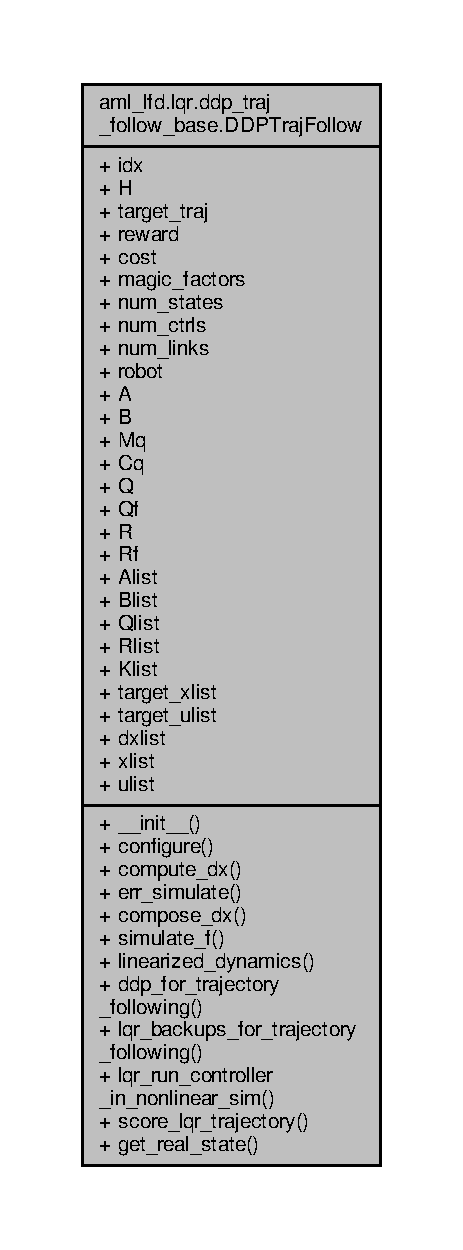
\includegraphics[height=550pt]{classaml__lfd_1_1lqr_1_1ddp__traj__follow__base_1_1_d_d_p_traj_follow__coll__graph}
\end{center}
\end{figure}
\subsection*{Public Member Functions}
\begin{DoxyCompactItemize}
\item 
\hypertarget{classaml__lfd_1_1lqr_1_1ddp__traj__follow__base_1_1_d_d_p_traj_follow_a056ad6c1307488c0ce377da8e5cf8bdb}{def {\bfseries \-\_\-\-\_\-init\-\_\-\-\_\-}}\label{classaml__lfd_1_1lqr_1_1ddp__traj__follow__base_1_1_d_d_p_traj_follow_a056ad6c1307488c0ce377da8e5cf8bdb}

\item 
\hypertarget{classaml__lfd_1_1lqr_1_1ddp__traj__follow__base_1_1_d_d_p_traj_follow_a90408dc24bbe915a9e95a87f1cc21d7d}{def {\bfseries configure}}\label{classaml__lfd_1_1lqr_1_1ddp__traj__follow__base_1_1_d_d_p_traj_follow_a90408dc24bbe915a9e95a87f1cc21d7d}

\item 
\hypertarget{classaml__lfd_1_1lqr_1_1ddp__traj__follow__base_1_1_d_d_p_traj_follow_a16dd3bb218fb2a761dedba0077ea5c75}{def {\bfseries compute\-\_\-dx}}\label{classaml__lfd_1_1lqr_1_1ddp__traj__follow__base_1_1_d_d_p_traj_follow_a16dd3bb218fb2a761dedba0077ea5c75}

\item 
\hypertarget{classaml__lfd_1_1lqr_1_1ddp__traj__follow__base_1_1_d_d_p_traj_follow_a29454de12b3272d19d31f1b9763a8c84}{def {\bfseries err\-\_\-simulate}}\label{classaml__lfd_1_1lqr_1_1ddp__traj__follow__base_1_1_d_d_p_traj_follow_a29454de12b3272d19d31f1b9763a8c84}

\item 
\hypertarget{classaml__lfd_1_1lqr_1_1ddp__traj__follow__base_1_1_d_d_p_traj_follow_a8aeae647129bd99e45a5601eaffa6ae9}{def {\bfseries compose\-\_\-dx}}\label{classaml__lfd_1_1lqr_1_1ddp__traj__follow__base_1_1_d_d_p_traj_follow_a8aeae647129bd99e45a5601eaffa6ae9}

\item 
\hypertarget{classaml__lfd_1_1lqr_1_1ddp__traj__follow__base_1_1_d_d_p_traj_follow_af7d1f720102dc0a16ab0e0259fee6bd4}{def {\bfseries simulate\-\_\-f}}\label{classaml__lfd_1_1lqr_1_1ddp__traj__follow__base_1_1_d_d_p_traj_follow_af7d1f720102dc0a16ab0e0259fee6bd4}

\item 
\hypertarget{classaml__lfd_1_1lqr_1_1ddp__traj__follow__base_1_1_d_d_p_traj_follow_ad99452c989bdd3f69793bf9d47060aab}{def {\bfseries linearized\-\_\-dynamics}}\label{classaml__lfd_1_1lqr_1_1ddp__traj__follow__base_1_1_d_d_p_traj_follow_ad99452c989bdd3f69793bf9d47060aab}

\item 
\hypertarget{classaml__lfd_1_1lqr_1_1ddp__traj__follow__base_1_1_d_d_p_traj_follow_adbd0641ee97f6f570336cba071f2e491}{def {\bfseries ddp\-\_\-for\-\_\-trajectory\-\_\-following}}\label{classaml__lfd_1_1lqr_1_1ddp__traj__follow__base_1_1_d_d_p_traj_follow_adbd0641ee97f6f570336cba071f2e491}

\item 
\hypertarget{classaml__lfd_1_1lqr_1_1ddp__traj__follow__base_1_1_d_d_p_traj_follow_a1d87e2ffffb673f72cf13b55c6d81846}{def {\bfseries lqr\-\_\-backups\-\_\-for\-\_\-trajectory\-\_\-following}}\label{classaml__lfd_1_1lqr_1_1ddp__traj__follow__base_1_1_d_d_p_traj_follow_a1d87e2ffffb673f72cf13b55c6d81846}

\item 
\hypertarget{classaml__lfd_1_1lqr_1_1ddp__traj__follow__base_1_1_d_d_p_traj_follow_aece8a96b5eb3535ef06ebc70a248eea9}{def {\bfseries lqr\-\_\-run\-\_\-controller\-\_\-in\-\_\-nonlinear\-\_\-sim}}\label{classaml__lfd_1_1lqr_1_1ddp__traj__follow__base_1_1_d_d_p_traj_follow_aece8a96b5eb3535ef06ebc70a248eea9}

\item 
\hypertarget{classaml__lfd_1_1lqr_1_1ddp__traj__follow__base_1_1_d_d_p_traj_follow_a21f0b4c8898671073bd6cdd2c8347e29}{def {\bfseries score\-\_\-lqr\-\_\-trajectory}}\label{classaml__lfd_1_1lqr_1_1ddp__traj__follow__base_1_1_d_d_p_traj_follow_a21f0b4c8898671073bd6cdd2c8347e29}

\item 
\hypertarget{classaml__lfd_1_1lqr_1_1ddp__traj__follow__base_1_1_d_d_p_traj_follow_ab064db58d2709906da9fdb29aee40a93}{def {\bfseries get\-\_\-real\-\_\-state}}\label{classaml__lfd_1_1lqr_1_1ddp__traj__follow__base_1_1_d_d_p_traj_follow_ab064db58d2709906da9fdb29aee40a93}

\end{DoxyCompactItemize}
\subsection*{Public Attributes}
\begin{DoxyCompactItemize}
\item 
\hypertarget{classaml__lfd_1_1lqr_1_1ddp__traj__follow__base_1_1_d_d_p_traj_follow_af0b6fbbc185f857a746ca2981001e4fa}{{\bfseries idx}}\label{classaml__lfd_1_1lqr_1_1ddp__traj__follow__base_1_1_d_d_p_traj_follow_af0b6fbbc185f857a746ca2981001e4fa}

\item 
\hypertarget{classaml__lfd_1_1lqr_1_1ddp__traj__follow__base_1_1_d_d_p_traj_follow_aec1df18773cc7d2f37d95e9408d4748f}{{\bfseries H}}\label{classaml__lfd_1_1lqr_1_1ddp__traj__follow__base_1_1_d_d_p_traj_follow_aec1df18773cc7d2f37d95e9408d4748f}

\item 
\hypertarget{classaml__lfd_1_1lqr_1_1ddp__traj__follow__base_1_1_d_d_p_traj_follow_a03f52d1545917a8954bd837c9fc428f8}{{\bfseries target\-\_\-traj}}\label{classaml__lfd_1_1lqr_1_1ddp__traj__follow__base_1_1_d_d_p_traj_follow_a03f52d1545917a8954bd837c9fc428f8}

\item 
\hypertarget{classaml__lfd_1_1lqr_1_1ddp__traj__follow__base_1_1_d_d_p_traj_follow_a1f8edf414c5f464fca690964c2a9bf7a}{{\bfseries reward}}\label{classaml__lfd_1_1lqr_1_1ddp__traj__follow__base_1_1_d_d_p_traj_follow_a1f8edf414c5f464fca690964c2a9bf7a}

\item 
\hypertarget{classaml__lfd_1_1lqr_1_1ddp__traj__follow__base_1_1_d_d_p_traj_follow_a843d69188b565822569099d0832f2b60}{{\bfseries cost}}\label{classaml__lfd_1_1lqr_1_1ddp__traj__follow__base_1_1_d_d_p_traj_follow_a843d69188b565822569099d0832f2b60}

\item 
\hypertarget{classaml__lfd_1_1lqr_1_1ddp__traj__follow__base_1_1_d_d_p_traj_follow_a76562065147ed65895d58af5f78b9e3b}{{\bfseries magic\-\_\-factors}}\label{classaml__lfd_1_1lqr_1_1ddp__traj__follow__base_1_1_d_d_p_traj_follow_a76562065147ed65895d58af5f78b9e3b}

\item 
\hypertarget{classaml__lfd_1_1lqr_1_1ddp__traj__follow__base_1_1_d_d_p_traj_follow_a3ff02e2708357534cb2af0d8a7e5560d}{{\bfseries num\-\_\-states}}\label{classaml__lfd_1_1lqr_1_1ddp__traj__follow__base_1_1_d_d_p_traj_follow_a3ff02e2708357534cb2af0d8a7e5560d}

\item 
\hypertarget{classaml__lfd_1_1lqr_1_1ddp__traj__follow__base_1_1_d_d_p_traj_follow_ac565b2592399d6c46eaa9603649e8bd1}{{\bfseries num\-\_\-ctrls}}\label{classaml__lfd_1_1lqr_1_1ddp__traj__follow__base_1_1_d_d_p_traj_follow_ac565b2592399d6c46eaa9603649e8bd1}

\item 
\hypertarget{classaml__lfd_1_1lqr_1_1ddp__traj__follow__base_1_1_d_d_p_traj_follow_a4cfe2bc27d78ce4dd4f96f591e812386}{{\bfseries num\-\_\-links}}\label{classaml__lfd_1_1lqr_1_1ddp__traj__follow__base_1_1_d_d_p_traj_follow_a4cfe2bc27d78ce4dd4f96f591e812386}

\item 
\hypertarget{classaml__lfd_1_1lqr_1_1ddp__traj__follow__base_1_1_d_d_p_traj_follow_a9bc25164edb2c2e29743ed1a8eb64488}{{\bfseries robot}}\label{classaml__lfd_1_1lqr_1_1ddp__traj__follow__base_1_1_d_d_p_traj_follow_a9bc25164edb2c2e29743ed1a8eb64488}

\item 
\hypertarget{classaml__lfd_1_1lqr_1_1ddp__traj__follow__base_1_1_d_d_p_traj_follow_ad7d04202fc2d76e5a955e5ffb71633cd}{{\bfseries A}}\label{classaml__lfd_1_1lqr_1_1ddp__traj__follow__base_1_1_d_d_p_traj_follow_ad7d04202fc2d76e5a955e5ffb71633cd}

\item 
\hypertarget{classaml__lfd_1_1lqr_1_1ddp__traj__follow__base_1_1_d_d_p_traj_follow_a63516b4578bc9ae85b609c7b1d8cc8db}{{\bfseries B}}\label{classaml__lfd_1_1lqr_1_1ddp__traj__follow__base_1_1_d_d_p_traj_follow_a63516b4578bc9ae85b609c7b1d8cc8db}

\item 
\hypertarget{classaml__lfd_1_1lqr_1_1ddp__traj__follow__base_1_1_d_d_p_traj_follow_a2dd2df27d2b4ea3cd0a91db3fda4427a}{{\bfseries Mq}}\label{classaml__lfd_1_1lqr_1_1ddp__traj__follow__base_1_1_d_d_p_traj_follow_a2dd2df27d2b4ea3cd0a91db3fda4427a}

\item 
\hypertarget{classaml__lfd_1_1lqr_1_1ddp__traj__follow__base_1_1_d_d_p_traj_follow_a0b0e42bc2ff3b66681542f8d8c38e100}{{\bfseries Cq}}\label{classaml__lfd_1_1lqr_1_1ddp__traj__follow__base_1_1_d_d_p_traj_follow_a0b0e42bc2ff3b66681542f8d8c38e100}

\item 
\hypertarget{classaml__lfd_1_1lqr_1_1ddp__traj__follow__base_1_1_d_d_p_traj_follow_a1173c1b05d86aa568abcab18b7bd69ea}{{\bfseries Q}}\label{classaml__lfd_1_1lqr_1_1ddp__traj__follow__base_1_1_d_d_p_traj_follow_a1173c1b05d86aa568abcab18b7bd69ea}

\item 
\hypertarget{classaml__lfd_1_1lqr_1_1ddp__traj__follow__base_1_1_d_d_p_traj_follow_abf905d9982f96f9ed454961c42359f9f}{{\bfseries Qf}}\label{classaml__lfd_1_1lqr_1_1ddp__traj__follow__base_1_1_d_d_p_traj_follow_abf905d9982f96f9ed454961c42359f9f}

\item 
\hypertarget{classaml__lfd_1_1lqr_1_1ddp__traj__follow__base_1_1_d_d_p_traj_follow_a70e3c8b1d5e33f94e5141075ebf02975}{{\bfseries R}}\label{classaml__lfd_1_1lqr_1_1ddp__traj__follow__base_1_1_d_d_p_traj_follow_a70e3c8b1d5e33f94e5141075ebf02975}

\item 
\hypertarget{classaml__lfd_1_1lqr_1_1ddp__traj__follow__base_1_1_d_d_p_traj_follow_a6c6bfb30d6a4c345412210240fb0e296}{{\bfseries Rf}}\label{classaml__lfd_1_1lqr_1_1ddp__traj__follow__base_1_1_d_d_p_traj_follow_a6c6bfb30d6a4c345412210240fb0e296}

\item 
\hypertarget{classaml__lfd_1_1lqr_1_1ddp__traj__follow__base_1_1_d_d_p_traj_follow_a577e00ce473a24465c4f0de0a146ef3e}{{\bfseries Alist}}\label{classaml__lfd_1_1lqr_1_1ddp__traj__follow__base_1_1_d_d_p_traj_follow_a577e00ce473a24465c4f0de0a146ef3e}

\item 
\hypertarget{classaml__lfd_1_1lqr_1_1ddp__traj__follow__base_1_1_d_d_p_traj_follow_a5da728040bfb20c0144f91e4e3f8cb36}{{\bfseries Blist}}\label{classaml__lfd_1_1lqr_1_1ddp__traj__follow__base_1_1_d_d_p_traj_follow_a5da728040bfb20c0144f91e4e3f8cb36}

\item 
\hypertarget{classaml__lfd_1_1lqr_1_1ddp__traj__follow__base_1_1_d_d_p_traj_follow_aeee69abfc8dd387e0ef2b752be44f2f6}{{\bfseries Qlist}}\label{classaml__lfd_1_1lqr_1_1ddp__traj__follow__base_1_1_d_d_p_traj_follow_aeee69abfc8dd387e0ef2b752be44f2f6}

\item 
\hypertarget{classaml__lfd_1_1lqr_1_1ddp__traj__follow__base_1_1_d_d_p_traj_follow_ae4c9a614b6a275e49e6f39bcb76b27b6}{{\bfseries Rlist}}\label{classaml__lfd_1_1lqr_1_1ddp__traj__follow__base_1_1_d_d_p_traj_follow_ae4c9a614b6a275e49e6f39bcb76b27b6}

\item 
\hypertarget{classaml__lfd_1_1lqr_1_1ddp__traj__follow__base_1_1_d_d_p_traj_follow_a1fc53a0218dd657abe54fa4585c35cd1}{{\bfseries Klist}}\label{classaml__lfd_1_1lqr_1_1ddp__traj__follow__base_1_1_d_d_p_traj_follow_a1fc53a0218dd657abe54fa4585c35cd1}

\item 
\hypertarget{classaml__lfd_1_1lqr_1_1ddp__traj__follow__base_1_1_d_d_p_traj_follow_ac8045400042e1740c62cd987a5bd78be}{{\bfseries target\-\_\-xlist}}\label{classaml__lfd_1_1lqr_1_1ddp__traj__follow__base_1_1_d_d_p_traj_follow_ac8045400042e1740c62cd987a5bd78be}

\item 
\hypertarget{classaml__lfd_1_1lqr_1_1ddp__traj__follow__base_1_1_d_d_p_traj_follow_af8fb8b26f0014cc318a822a1ecce6859}{{\bfseries target\-\_\-ulist}}\label{classaml__lfd_1_1lqr_1_1ddp__traj__follow__base_1_1_d_d_p_traj_follow_af8fb8b26f0014cc318a822a1ecce6859}

\item 
\hypertarget{classaml__lfd_1_1lqr_1_1ddp__traj__follow__base_1_1_d_d_p_traj_follow_a6d2157818c66fe4ca6c57414262309a4}{{\bfseries dxlist}}\label{classaml__lfd_1_1lqr_1_1ddp__traj__follow__base_1_1_d_d_p_traj_follow_a6d2157818c66fe4ca6c57414262309a4}

\item 
\hypertarget{classaml__lfd_1_1lqr_1_1ddp__traj__follow__base_1_1_d_d_p_traj_follow_a737296883bc4be3b617e584833125ed3}{{\bfseries xlist}}\label{classaml__lfd_1_1lqr_1_1ddp__traj__follow__base_1_1_d_d_p_traj_follow_a737296883bc4be3b617e584833125ed3}

\item 
\hypertarget{classaml__lfd_1_1lqr_1_1ddp__traj__follow__base_1_1_d_d_p_traj_follow_a23c501383ace126e72954a4e9e3138f1}{{\bfseries ulist}}\label{classaml__lfd_1_1lqr_1_1ddp__traj__follow__base_1_1_d_d_p_traj_follow_a23c501383ace126e72954a4e9e3138f1}

\end{DoxyCompactItemize}


The documentation for this class was generated from the following file\-:\begin{DoxyCompactItemize}
\item 
aml\-\_\-lfd/src/aml\-\_\-lfd/lqr/ddp\-\_\-traj\-\_\-follow\-\_\-base.\-py\end{DoxyCompactItemize}

\hypertarget{classaml__lfd_1_1dmp_1_1discrete__dmp__shell_1_1_discrete_d_m_p_shell}{}\section{aml\+\_\+lfd.\+dmp.\+discrete\+\_\+dmp\+\_\+shell.\+Discrete\+D\+M\+P\+Shell Class Reference}
\label{classaml__lfd_1_1dmp_1_1discrete__dmp__shell_1_1_discrete_d_m_p_shell}\index{aml\+\_\+lfd.\+dmp.\+discrete\+\_\+dmp\+\_\+shell.\+Discrete\+D\+M\+P\+Shell@{aml\+\_\+lfd.\+dmp.\+discrete\+\_\+dmp\+\_\+shell.\+Discrete\+D\+M\+P\+Shell}}


Inheritance diagram for aml\+\_\+lfd.\+dmp.\+discrete\+\_\+dmp\+\_\+shell.\+Discrete\+D\+M\+P\+Shell\+:\nopagebreak
\begin{figure}[H]
\begin{center}
\leavevmode
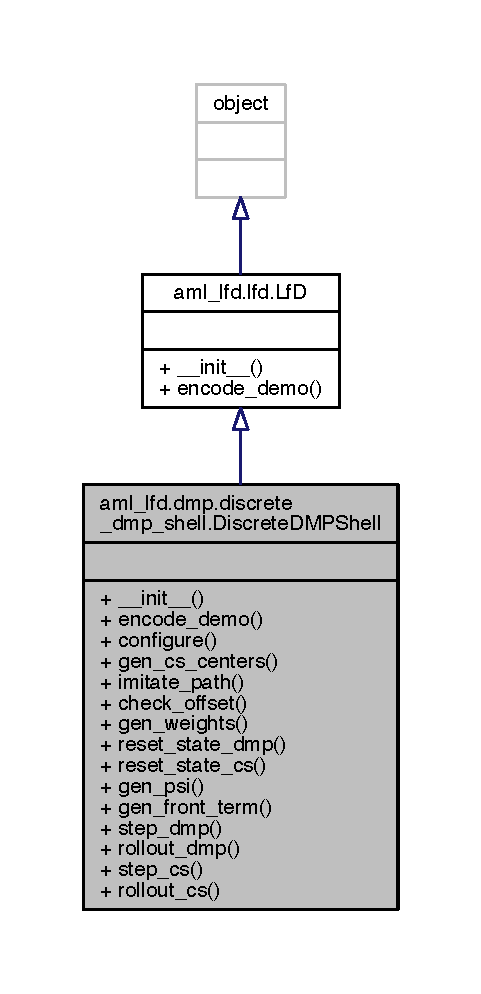
\includegraphics[width=231pt]{classaml__lfd_1_1dmp_1_1discrete__dmp__shell_1_1_discrete_d_m_p_shell__inherit__graph}
\end{center}
\end{figure}


Collaboration diagram for aml\+\_\+lfd.\+dmp.\+discrete\+\_\+dmp\+\_\+shell.\+Discrete\+D\+M\+P\+Shell\+:\nopagebreak
\begin{figure}[H]
\begin{center}
\leavevmode
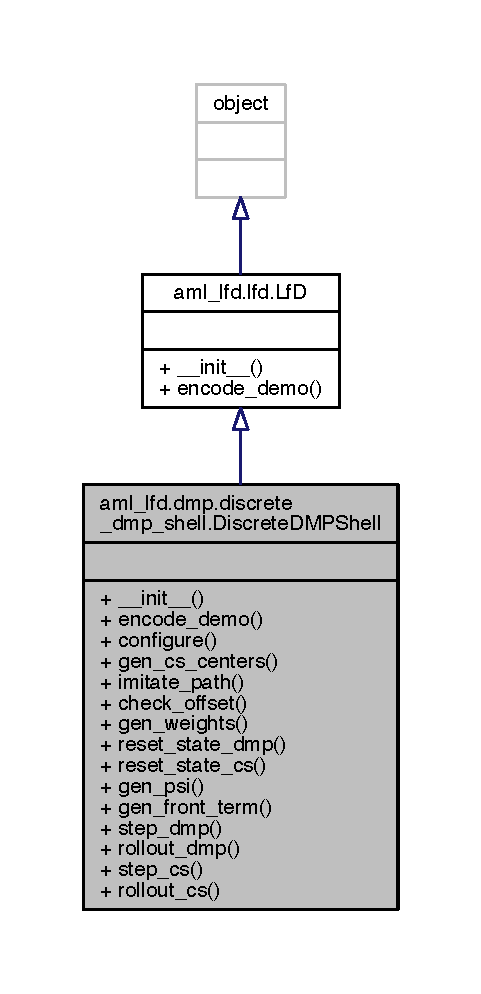
\includegraphics[width=231pt]{classaml__lfd_1_1dmp_1_1discrete__dmp__shell_1_1_discrete_d_m_p_shell__coll__graph}
\end{center}
\end{figure}
\subsection*{Public Member Functions}
\begin{DoxyCompactItemize}
\item 
\hypertarget{classaml__lfd_1_1dmp_1_1discrete__dmp__shell_1_1_discrete_d_m_p_shell_afdc79719c645bf1ffd4166faff1ce082}{}\label{classaml__lfd_1_1dmp_1_1discrete__dmp__shell_1_1_discrete_d_m_p_shell_afdc79719c645bf1ffd4166faff1ce082} 
def {\bfseries \+\_\+\+\_\+init\+\_\+\+\_\+} (self, config=D\+I\+S\+C\+R\+E\+T\+E\+\_\+\+D\+MP)
\item 
\hypertarget{classaml__lfd_1_1dmp_1_1discrete__dmp__shell_1_1_discrete_d_m_p_shell_a8e9bcf0d7885c2b6e8bef7b57ea3ffbe}{}\label{classaml__lfd_1_1dmp_1_1discrete__dmp__shell_1_1_discrete_d_m_p_shell_a8e9bcf0d7885c2b6e8bef7b57ea3ffbe} 
def {\bfseries encode\+\_\+demo} (self)
\item 
\hypertarget{classaml__lfd_1_1dmp_1_1discrete__dmp__shell_1_1_discrete_d_m_p_shell_a5d15a53724bb01efe93bc3a176837458}{}\label{classaml__lfd_1_1dmp_1_1discrete__dmp__shell_1_1_discrete_d_m_p_shell_a5d15a53724bb01efe93bc3a176837458} 
def {\bfseries configure} (self, traj2follow, start, goal)
\item 
def \hyperlink{classaml__lfd_1_1dmp_1_1discrete__dmp__shell_1_1_discrete_d_m_p_shell_ab364e2625c5983ba748c212e7cc4b16b}{gen\+\_\+cs\+\_\+centers} (self)
\item 
def \hyperlink{classaml__lfd_1_1dmp_1_1discrete__dmp__shell_1_1_discrete_d_m_p_shell_a2036e592bfd791bf24f238f9636b42ff}{imitate\+\_\+path} (self)
\item 
def \hyperlink{classaml__lfd_1_1dmp_1_1discrete__dmp__shell_1_1_discrete_d_m_p_shell_a10cec75150acb1c2e426fc17ce22bde6}{check\+\_\+offset} (self)
\item 
def \hyperlink{classaml__lfd_1_1dmp_1_1discrete__dmp__shell_1_1_discrete_d_m_p_shell_a369eaa244df73de31517906315c98772}{gen\+\_\+weights} (self, f\+\_\+target)
\item 
def \hyperlink{classaml__lfd_1_1dmp_1_1discrete__dmp__shell_1_1_discrete_d_m_p_shell_a07482e8fe6955be1c72e67258953e298}{reset\+\_\+state\+\_\+dmp} (self, new\+\_\+start=None)
\item 
def \hyperlink{classaml__lfd_1_1dmp_1_1discrete__dmp__shell_1_1_discrete_d_m_p_shell_a26c7a072996b7b5e2cdb13f19e3c3053}{reset\+\_\+state\+\_\+cs} (self)
\item 
def \hyperlink{classaml__lfd_1_1dmp_1_1discrete__dmp__shell_1_1_discrete_d_m_p_shell_a0da4fbcdb74db7ca2d32e5913be72a81}{gen\+\_\+psi} (self, x)
\item 
def \hyperlink{classaml__lfd_1_1dmp_1_1discrete__dmp__shell_1_1_discrete_d_m_p_shell_a49cf27ca02e86e1773133835e1f606a2}{gen\+\_\+front\+\_\+term} (self, x, dmp\+\_\+num)
\item 
def \hyperlink{classaml__lfd_1_1dmp_1_1discrete__dmp__shell_1_1_discrete_d_m_p_shell_a198fd652ccf7f3d54a77361f521ca3ae}{step\+\_\+dmp} (self, tau=None, state\+\_\+fb=None, external\+\_\+force=None)
\item 
def \hyperlink{classaml__lfd_1_1dmp_1_1discrete__dmp__shell_1_1_discrete_d_m_p_shell_ad46fa7e783a6c38e19bb6f36fed76a8b}{rollout\+\_\+dmp} (self, tau=None)
\item 
def \hyperlink{classaml__lfd_1_1dmp_1_1discrete__dmp__shell_1_1_discrete_d_m_p_shell_aeff4509250d19885d751a439f3eff8f5}{step\+\_\+cs} (self, tau=1.\+0, error\+\_\+coupling=1.\+0)
\item 
def \hyperlink{classaml__lfd_1_1dmp_1_1discrete__dmp__shell_1_1_discrete_d_m_p_shell_a21a2c8cac5774e8dbd87a211fda6ef05}{rollout\+\_\+cs} (self, kwargs)
\end{DoxyCompactItemize}


\subsection{Member Function Documentation}
\hypertarget{classaml__lfd_1_1dmp_1_1discrete__dmp__shell_1_1_discrete_d_m_p_shell_a10cec75150acb1c2e426fc17ce22bde6}{}\label{classaml__lfd_1_1dmp_1_1discrete__dmp__shell_1_1_discrete_d_m_p_shell_a10cec75150acb1c2e426fc17ce22bde6} 
\index{aml\+\_\+lfd\+::dmp\+::discrete\+\_\+dmp\+\_\+shell\+::\+Discrete\+D\+M\+P\+Shell@{aml\+\_\+lfd\+::dmp\+::discrete\+\_\+dmp\+\_\+shell\+::\+Discrete\+D\+M\+P\+Shell}!check\+\_\+offset@{check\+\_\+offset}}
\index{check\+\_\+offset@{check\+\_\+offset}!aml\+\_\+lfd\+::dmp\+::discrete\+\_\+dmp\+\_\+shell\+::\+Discrete\+D\+M\+P\+Shell@{aml\+\_\+lfd\+::dmp\+::discrete\+\_\+dmp\+\_\+shell\+::\+Discrete\+D\+M\+P\+Shell}}
\subsubsection{\texorpdfstring{check\+\_\+offset()}{check\_offset()}}
{\footnotesize\ttfamily def aml\+\_\+lfd.\+dmp.\+discrete\+\_\+dmp\+\_\+shell.\+Discrete\+D\+M\+P\+Shell.\+check\+\_\+offset (\begin{DoxyParamCaption}\item[{}]{self }\end{DoxyParamCaption})}

\begin{DoxyVerb}Check to see if initial position and goal are the same
if they are, offset slightly so that the forcing term is not 0\end{DoxyVerb}
 \hypertarget{classaml__lfd_1_1dmp_1_1discrete__dmp__shell_1_1_discrete_d_m_p_shell_ab364e2625c5983ba748c212e7cc4b16b}{}\label{classaml__lfd_1_1dmp_1_1discrete__dmp__shell_1_1_discrete_d_m_p_shell_ab364e2625c5983ba748c212e7cc4b16b} 
\index{aml\+\_\+lfd\+::dmp\+::discrete\+\_\+dmp\+\_\+shell\+::\+Discrete\+D\+M\+P\+Shell@{aml\+\_\+lfd\+::dmp\+::discrete\+\_\+dmp\+\_\+shell\+::\+Discrete\+D\+M\+P\+Shell}!gen\+\_\+cs\+\_\+centers@{gen\+\_\+cs\+\_\+centers}}
\index{gen\+\_\+cs\+\_\+centers@{gen\+\_\+cs\+\_\+centers}!aml\+\_\+lfd\+::dmp\+::discrete\+\_\+dmp\+\_\+shell\+::\+Discrete\+D\+M\+P\+Shell@{aml\+\_\+lfd\+::dmp\+::discrete\+\_\+dmp\+\_\+shell\+::\+Discrete\+D\+M\+P\+Shell}}
\subsubsection{\texorpdfstring{gen\+\_\+cs\+\_\+centers()}{gen\_cs\_centers()}}
{\footnotesize\ttfamily def aml\+\_\+lfd.\+dmp.\+discrete\+\_\+dmp\+\_\+shell.\+Discrete\+D\+M\+P\+Shell.\+gen\+\_\+cs\+\_\+centers (\begin{DoxyParamCaption}\item[{}]{self }\end{DoxyParamCaption})}

\begin{DoxyVerb}Set the centre of the Gaussian basis 
functions be spaced evenly throughout run time\end{DoxyVerb}
 \hypertarget{classaml__lfd_1_1dmp_1_1discrete__dmp__shell_1_1_discrete_d_m_p_shell_a49cf27ca02e86e1773133835e1f606a2}{}\label{classaml__lfd_1_1dmp_1_1discrete__dmp__shell_1_1_discrete_d_m_p_shell_a49cf27ca02e86e1773133835e1f606a2} 
\index{aml\+\_\+lfd\+::dmp\+::discrete\+\_\+dmp\+\_\+shell\+::\+Discrete\+D\+M\+P\+Shell@{aml\+\_\+lfd\+::dmp\+::discrete\+\_\+dmp\+\_\+shell\+::\+Discrete\+D\+M\+P\+Shell}!gen\+\_\+front\+\_\+term@{gen\+\_\+front\+\_\+term}}
\index{gen\+\_\+front\+\_\+term@{gen\+\_\+front\+\_\+term}!aml\+\_\+lfd\+::dmp\+::discrete\+\_\+dmp\+\_\+shell\+::\+Discrete\+D\+M\+P\+Shell@{aml\+\_\+lfd\+::dmp\+::discrete\+\_\+dmp\+\_\+shell\+::\+Discrete\+D\+M\+P\+Shell}}
\subsubsection{\texorpdfstring{gen\+\_\+front\+\_\+term()}{gen\_front\_term()}}
{\footnotesize\ttfamily def aml\+\_\+lfd.\+dmp.\+discrete\+\_\+dmp\+\_\+shell.\+Discrete\+D\+M\+P\+Shell.\+gen\+\_\+front\+\_\+term (\begin{DoxyParamCaption}\item[{}]{self,  }\item[{}]{x,  }\item[{}]{dmp\+\_\+num }\end{DoxyParamCaption})}

\begin{DoxyVerb}Generates the diminishing front term on 
the forcing term.

x float: the current value of the canonical system
dmp_num int: the index of the current dmp
\end{DoxyVerb}
 \hypertarget{classaml__lfd_1_1dmp_1_1discrete__dmp__shell_1_1_discrete_d_m_p_shell_a0da4fbcdb74db7ca2d32e5913be72a81}{}\label{classaml__lfd_1_1dmp_1_1discrete__dmp__shell_1_1_discrete_d_m_p_shell_a0da4fbcdb74db7ca2d32e5913be72a81} 
\index{aml\+\_\+lfd\+::dmp\+::discrete\+\_\+dmp\+\_\+shell\+::\+Discrete\+D\+M\+P\+Shell@{aml\+\_\+lfd\+::dmp\+::discrete\+\_\+dmp\+\_\+shell\+::\+Discrete\+D\+M\+P\+Shell}!gen\+\_\+psi@{gen\+\_\+psi}}
\index{gen\+\_\+psi@{gen\+\_\+psi}!aml\+\_\+lfd\+::dmp\+::discrete\+\_\+dmp\+\_\+shell\+::\+Discrete\+D\+M\+P\+Shell@{aml\+\_\+lfd\+::dmp\+::discrete\+\_\+dmp\+\_\+shell\+::\+Discrete\+D\+M\+P\+Shell}}
\subsubsection{\texorpdfstring{gen\+\_\+psi()}{gen\_psi()}}
{\footnotesize\ttfamily def aml\+\_\+lfd.\+dmp.\+discrete\+\_\+dmp\+\_\+shell.\+Discrete\+D\+M\+P\+Shell.\+gen\+\_\+psi (\begin{DoxyParamCaption}\item[{}]{self,  }\item[{}]{x }\end{DoxyParamCaption})}

\begin{DoxyVerb}Generates the activity of the basis functions for a given 
canonical system rollout. 

x float, array: the canonical system state or path
\end{DoxyVerb}
 \hypertarget{classaml__lfd_1_1dmp_1_1discrete__dmp__shell_1_1_discrete_d_m_p_shell_a369eaa244df73de31517906315c98772}{}\label{classaml__lfd_1_1dmp_1_1discrete__dmp__shell_1_1_discrete_d_m_p_shell_a369eaa244df73de31517906315c98772} 
\index{aml\+\_\+lfd\+::dmp\+::discrete\+\_\+dmp\+\_\+shell\+::\+Discrete\+D\+M\+P\+Shell@{aml\+\_\+lfd\+::dmp\+::discrete\+\_\+dmp\+\_\+shell\+::\+Discrete\+D\+M\+P\+Shell}!gen\+\_\+weights@{gen\+\_\+weights}}
\index{gen\+\_\+weights@{gen\+\_\+weights}!aml\+\_\+lfd\+::dmp\+::discrete\+\_\+dmp\+\_\+shell\+::\+Discrete\+D\+M\+P\+Shell@{aml\+\_\+lfd\+::dmp\+::discrete\+\_\+dmp\+\_\+shell\+::\+Discrete\+D\+M\+P\+Shell}}
\subsubsection{\texorpdfstring{gen\+\_\+weights()}{gen\_weights()}}
{\footnotesize\ttfamily def aml\+\_\+lfd.\+dmp.\+discrete\+\_\+dmp\+\_\+shell.\+Discrete\+D\+M\+P\+Shell.\+gen\+\_\+weights (\begin{DoxyParamCaption}\item[{}]{self,  }\item[{}]{f\+\_\+target }\end{DoxyParamCaption})}

\begin{DoxyVerb}Generate a set of weights over the basis functions such 
that the target forcing term trajectory is matched.

f_target np.array: the desired forcing term trajectory
\end{DoxyVerb}
 \hypertarget{classaml__lfd_1_1dmp_1_1discrete__dmp__shell_1_1_discrete_d_m_p_shell_a2036e592bfd791bf24f238f9636b42ff}{}\label{classaml__lfd_1_1dmp_1_1discrete__dmp__shell_1_1_discrete_d_m_p_shell_a2036e592bfd791bf24f238f9636b42ff} 
\index{aml\+\_\+lfd\+::dmp\+::discrete\+\_\+dmp\+\_\+shell\+::\+Discrete\+D\+M\+P\+Shell@{aml\+\_\+lfd\+::dmp\+::discrete\+\_\+dmp\+\_\+shell\+::\+Discrete\+D\+M\+P\+Shell}!imitate\+\_\+path@{imitate\+\_\+path}}
\index{imitate\+\_\+path@{imitate\+\_\+path}!aml\+\_\+lfd\+::dmp\+::discrete\+\_\+dmp\+\_\+shell\+::\+Discrete\+D\+M\+P\+Shell@{aml\+\_\+lfd\+::dmp\+::discrete\+\_\+dmp\+\_\+shell\+::\+Discrete\+D\+M\+P\+Shell}}
\subsubsection{\texorpdfstring{imitate\+\_\+path()}{imitate\_path()}}
{\footnotesize\ttfamily def aml\+\_\+lfd.\+dmp.\+discrete\+\_\+dmp\+\_\+shell.\+Discrete\+D\+M\+P\+Shell.\+imitate\+\_\+path (\begin{DoxyParamCaption}\item[{}]{self }\end{DoxyParamCaption})}

\begin{DoxyVerb}Takes in a desired trajectory and generates the set of 
system parameters that best realize this path.
    
y_des list/array: the desired trajectories of each DMP
          should be shaped [dmps, run_time]
\end{DoxyVerb}
 \hypertarget{classaml__lfd_1_1dmp_1_1discrete__dmp__shell_1_1_discrete_d_m_p_shell_a26c7a072996b7b5e2cdb13f19e3c3053}{}\label{classaml__lfd_1_1dmp_1_1discrete__dmp__shell_1_1_discrete_d_m_p_shell_a26c7a072996b7b5e2cdb13f19e3c3053} 
\index{aml\+\_\+lfd\+::dmp\+::discrete\+\_\+dmp\+\_\+shell\+::\+Discrete\+D\+M\+P\+Shell@{aml\+\_\+lfd\+::dmp\+::discrete\+\_\+dmp\+\_\+shell\+::\+Discrete\+D\+M\+P\+Shell}!reset\+\_\+state\+\_\+cs@{reset\+\_\+state\+\_\+cs}}
\index{reset\+\_\+state\+\_\+cs@{reset\+\_\+state\+\_\+cs}!aml\+\_\+lfd\+::dmp\+::discrete\+\_\+dmp\+\_\+shell\+::\+Discrete\+D\+M\+P\+Shell@{aml\+\_\+lfd\+::dmp\+::discrete\+\_\+dmp\+\_\+shell\+::\+Discrete\+D\+M\+P\+Shell}}
\subsubsection{\texorpdfstring{reset\+\_\+state\+\_\+cs()}{reset\_state\_cs()}}
{\footnotesize\ttfamily def aml\+\_\+lfd.\+dmp.\+discrete\+\_\+dmp\+\_\+shell.\+Discrete\+D\+M\+P\+Shell.\+reset\+\_\+state\+\_\+cs (\begin{DoxyParamCaption}\item[{}]{self }\end{DoxyParamCaption})}

\begin{DoxyVerb}Reset the system state\end{DoxyVerb}
 \hypertarget{classaml__lfd_1_1dmp_1_1discrete__dmp__shell_1_1_discrete_d_m_p_shell_a07482e8fe6955be1c72e67258953e298}{}\label{classaml__lfd_1_1dmp_1_1discrete__dmp__shell_1_1_discrete_d_m_p_shell_a07482e8fe6955be1c72e67258953e298} 
\index{aml\+\_\+lfd\+::dmp\+::discrete\+\_\+dmp\+\_\+shell\+::\+Discrete\+D\+M\+P\+Shell@{aml\+\_\+lfd\+::dmp\+::discrete\+\_\+dmp\+\_\+shell\+::\+Discrete\+D\+M\+P\+Shell}!reset\+\_\+state\+\_\+dmp@{reset\+\_\+state\+\_\+dmp}}
\index{reset\+\_\+state\+\_\+dmp@{reset\+\_\+state\+\_\+dmp}!aml\+\_\+lfd\+::dmp\+::discrete\+\_\+dmp\+\_\+shell\+::\+Discrete\+D\+M\+P\+Shell@{aml\+\_\+lfd\+::dmp\+::discrete\+\_\+dmp\+\_\+shell\+::\+Discrete\+D\+M\+P\+Shell}}
\subsubsection{\texorpdfstring{reset\+\_\+state\+\_\+dmp()}{reset\_state\_dmp()}}
{\footnotesize\ttfamily def aml\+\_\+lfd.\+dmp.\+discrete\+\_\+dmp\+\_\+shell.\+Discrete\+D\+M\+P\+Shell.\+reset\+\_\+state\+\_\+dmp (\begin{DoxyParamCaption}\item[{}]{self,  }\item[{}]{new\+\_\+start = {\ttfamily None} }\end{DoxyParamCaption})}

\begin{DoxyVerb}Reset the system state\end{DoxyVerb}
 \hypertarget{classaml__lfd_1_1dmp_1_1discrete__dmp__shell_1_1_discrete_d_m_p_shell_a21a2c8cac5774e8dbd87a211fda6ef05}{}\label{classaml__lfd_1_1dmp_1_1discrete__dmp__shell_1_1_discrete_d_m_p_shell_a21a2c8cac5774e8dbd87a211fda6ef05} 
\index{aml\+\_\+lfd\+::dmp\+::discrete\+\_\+dmp\+\_\+shell\+::\+Discrete\+D\+M\+P\+Shell@{aml\+\_\+lfd\+::dmp\+::discrete\+\_\+dmp\+\_\+shell\+::\+Discrete\+D\+M\+P\+Shell}!rollout\+\_\+cs@{rollout\+\_\+cs}}
\index{rollout\+\_\+cs@{rollout\+\_\+cs}!aml\+\_\+lfd\+::dmp\+::discrete\+\_\+dmp\+\_\+shell\+::\+Discrete\+D\+M\+P\+Shell@{aml\+\_\+lfd\+::dmp\+::discrete\+\_\+dmp\+\_\+shell\+::\+Discrete\+D\+M\+P\+Shell}}
\subsubsection{\texorpdfstring{rollout\+\_\+cs()}{rollout\_cs()}}
{\footnotesize\ttfamily def aml\+\_\+lfd.\+dmp.\+discrete\+\_\+dmp\+\_\+shell.\+Discrete\+D\+M\+P\+Shell.\+rollout\+\_\+cs (\begin{DoxyParamCaption}\item[{}]{self,  }\item[{}]{kwargs }\end{DoxyParamCaption})}

\begin{DoxyVerb}Generate x for open loop movements.
\end{DoxyVerb}
 \hypertarget{classaml__lfd_1_1dmp_1_1discrete__dmp__shell_1_1_discrete_d_m_p_shell_ad46fa7e783a6c38e19bb6f36fed76a8b}{}\label{classaml__lfd_1_1dmp_1_1discrete__dmp__shell_1_1_discrete_d_m_p_shell_ad46fa7e783a6c38e19bb6f36fed76a8b} 
\index{aml\+\_\+lfd\+::dmp\+::discrete\+\_\+dmp\+\_\+shell\+::\+Discrete\+D\+M\+P\+Shell@{aml\+\_\+lfd\+::dmp\+::discrete\+\_\+dmp\+\_\+shell\+::\+Discrete\+D\+M\+P\+Shell}!rollout\+\_\+dmp@{rollout\+\_\+dmp}}
\index{rollout\+\_\+dmp@{rollout\+\_\+dmp}!aml\+\_\+lfd\+::dmp\+::discrete\+\_\+dmp\+\_\+shell\+::\+Discrete\+D\+M\+P\+Shell@{aml\+\_\+lfd\+::dmp\+::discrete\+\_\+dmp\+\_\+shell\+::\+Discrete\+D\+M\+P\+Shell}}
\subsubsection{\texorpdfstring{rollout\+\_\+dmp()}{rollout\_dmp()}}
{\footnotesize\ttfamily def aml\+\_\+lfd.\+dmp.\+discrete\+\_\+dmp\+\_\+shell.\+Discrete\+D\+M\+P\+Shell.\+rollout\+\_\+dmp (\begin{DoxyParamCaption}\item[{}]{self,  }\item[{}]{tau = {\ttfamily None} }\end{DoxyParamCaption})}

\begin{DoxyVerb}Generate a system trial, no feedback is incorporated.\end{DoxyVerb}
 \hypertarget{classaml__lfd_1_1dmp_1_1discrete__dmp__shell_1_1_discrete_d_m_p_shell_aeff4509250d19885d751a439f3eff8f5}{}\label{classaml__lfd_1_1dmp_1_1discrete__dmp__shell_1_1_discrete_d_m_p_shell_aeff4509250d19885d751a439f3eff8f5} 
\index{aml\+\_\+lfd\+::dmp\+::discrete\+\_\+dmp\+\_\+shell\+::\+Discrete\+D\+M\+P\+Shell@{aml\+\_\+lfd\+::dmp\+::discrete\+\_\+dmp\+\_\+shell\+::\+Discrete\+D\+M\+P\+Shell}!step\+\_\+cs@{step\+\_\+cs}}
\index{step\+\_\+cs@{step\+\_\+cs}!aml\+\_\+lfd\+::dmp\+::discrete\+\_\+dmp\+\_\+shell\+::\+Discrete\+D\+M\+P\+Shell@{aml\+\_\+lfd\+::dmp\+::discrete\+\_\+dmp\+\_\+shell\+::\+Discrete\+D\+M\+P\+Shell}}
\subsubsection{\texorpdfstring{step\+\_\+cs()}{step\_cs()}}
{\footnotesize\ttfamily def aml\+\_\+lfd.\+dmp.\+discrete\+\_\+dmp\+\_\+shell.\+Discrete\+D\+M\+P\+Shell.\+step\+\_\+cs (\begin{DoxyParamCaption}\item[{}]{self,  }\item[{}]{tau = {\ttfamily 1.0},  }\item[{}]{error\+\_\+coupling = {\ttfamily 1.0} }\end{DoxyParamCaption})}

\begin{DoxyVerb}Generate a single step of x for discrete
(potentially closed) loop movements. 
Decaying from 1 to 0 according to dx = -ax*x.

tau float: gain on execution time
   increase tau to make the system execute faster
error_coupling float: slow down if the error is > 1
\end{DoxyVerb}
 \hypertarget{classaml__lfd_1_1dmp_1_1discrete__dmp__shell_1_1_discrete_d_m_p_shell_a198fd652ccf7f3d54a77361f521ca3ae}{}\label{classaml__lfd_1_1dmp_1_1discrete__dmp__shell_1_1_discrete_d_m_p_shell_a198fd652ccf7f3d54a77361f521ca3ae} 
\index{aml\+\_\+lfd\+::dmp\+::discrete\+\_\+dmp\+\_\+shell\+::\+Discrete\+D\+M\+P\+Shell@{aml\+\_\+lfd\+::dmp\+::discrete\+\_\+dmp\+\_\+shell\+::\+Discrete\+D\+M\+P\+Shell}!step\+\_\+dmp@{step\+\_\+dmp}}
\index{step\+\_\+dmp@{step\+\_\+dmp}!aml\+\_\+lfd\+::dmp\+::discrete\+\_\+dmp\+\_\+shell\+::\+Discrete\+D\+M\+P\+Shell@{aml\+\_\+lfd\+::dmp\+::discrete\+\_\+dmp\+\_\+shell\+::\+Discrete\+D\+M\+P\+Shell}}
\subsubsection{\texorpdfstring{step\+\_\+dmp()}{step\_dmp()}}
{\footnotesize\ttfamily def aml\+\_\+lfd.\+dmp.\+discrete\+\_\+dmp\+\_\+shell.\+Discrete\+D\+M\+P\+Shell.\+step\+\_\+dmp (\begin{DoxyParamCaption}\item[{}]{self,  }\item[{}]{tau = {\ttfamily None},  }\item[{}]{state\+\_\+fb = {\ttfamily None},  }\item[{}]{external\+\_\+force = {\ttfamily None} }\end{DoxyParamCaption})}

\begin{DoxyVerb}Run the DMP system for a single timestep.

       tau float: scales the timestep
  increase tau to make the system execute faster
       state_fb np.array: optional system feedback
\end{DoxyVerb}
 

The documentation for this class was generated from the following file\+:\begin{DoxyCompactItemize}
\item 
aml\+\_\+lfd/src/aml\+\_\+lfd/dmp/discrete\+\_\+dmp\+\_\+shell.\+py\end{DoxyCompactItemize}

\hypertarget{classtest__record__sample_1_1_dummy_task_interface}{}\section{test\+\_\+record\+\_\+sample.\+Dummy\+Task\+Interface Class Reference}
\label{classtest__record__sample_1_1_dummy_task_interface}\index{test\+\_\+record\+\_\+sample.\+Dummy\+Task\+Interface@{test\+\_\+record\+\_\+sample.\+Dummy\+Task\+Interface}}


Inheritance diagram for test\+\_\+record\+\_\+sample.\+Dummy\+Task\+Interface\+:\nopagebreak
\begin{figure}[H]
\begin{center}
\leavevmode
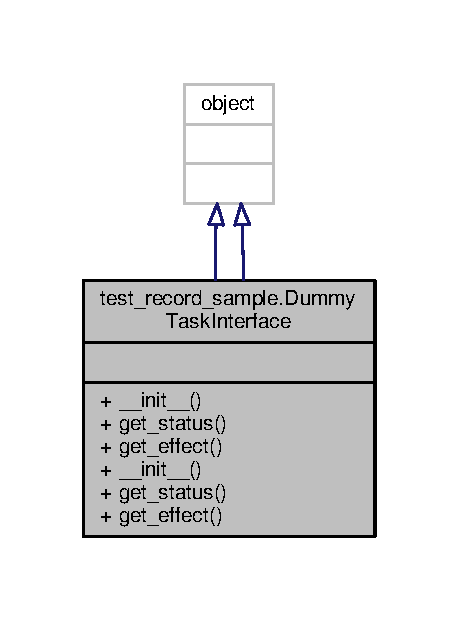
\includegraphics[width=221pt]{classtest__record__sample_1_1_dummy_task_interface__inherit__graph}
\end{center}
\end{figure}


Collaboration diagram for test\+\_\+record\+\_\+sample.\+Dummy\+Task\+Interface\+:\nopagebreak
\begin{figure}[H]
\begin{center}
\leavevmode
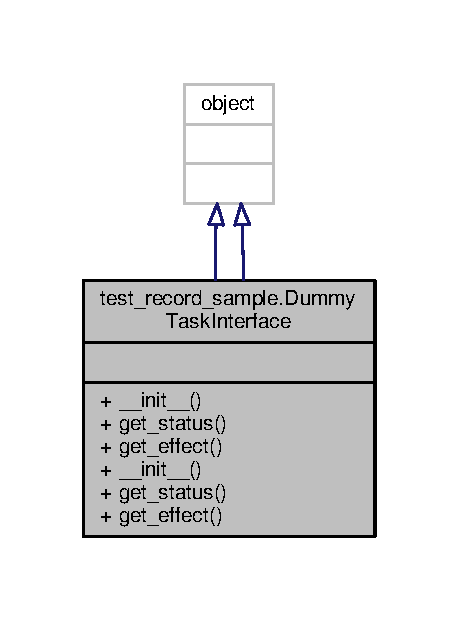
\includegraphics[width=221pt]{classtest__record__sample_1_1_dummy_task_interface__coll__graph}
\end{center}
\end{figure}
\subsection*{Public Member Functions}
\begin{DoxyCompactItemize}
\item 
\hypertarget{classtest__record__sample_1_1_dummy_task_interface_ae65615d7e6bf3cabcbaa38c704ad3e8e}{}\label{classtest__record__sample_1_1_dummy_task_interface_ae65615d7e6bf3cabcbaa38c704ad3e8e} 
def {\bfseries \+\_\+\+\_\+init\+\_\+\+\_\+} (self)
\item 
\hypertarget{classtest__record__sample_1_1_dummy_task_interface_a5f30dff815bef801f930219a68e01a34}{}\label{classtest__record__sample_1_1_dummy_task_interface_a5f30dff815bef801f930219a68e01a34} 
def {\bfseries get\+\_\+status} (self)
\item 
\hypertarget{classtest__record__sample_1_1_dummy_task_interface_abb169f22038abe7de80434e898d219e3}{}\label{classtest__record__sample_1_1_dummy_task_interface_abb169f22038abe7de80434e898d219e3} 
def {\bfseries get\+\_\+effect} (self)
\item 
\hypertarget{classtest__record__sample_1_1_dummy_task_interface_ae65615d7e6bf3cabcbaa38c704ad3e8e}{}\label{classtest__record__sample_1_1_dummy_task_interface_ae65615d7e6bf3cabcbaa38c704ad3e8e} 
def {\bfseries \+\_\+\+\_\+init\+\_\+\+\_\+} (self)
\item 
\hypertarget{classtest__record__sample_1_1_dummy_task_interface_a5f30dff815bef801f930219a68e01a34}{}\label{classtest__record__sample_1_1_dummy_task_interface_a5f30dff815bef801f930219a68e01a34} 
def {\bfseries get\+\_\+status} (self)
\item 
\hypertarget{classtest__record__sample_1_1_dummy_task_interface_abb169f22038abe7de80434e898d219e3}{}\label{classtest__record__sample_1_1_dummy_task_interface_abb169f22038abe7de80434e898d219e3} 
def {\bfseries get\+\_\+effect} (self)
\end{DoxyCompactItemize}


The documentation for this class was generated from the following file\+:\begin{DoxyCompactItemize}
\item 
aml\+\_\+data\+\_\+collec\+\_\+utils/src/aml\+\_\+data\+\_\+collec\+\_\+utils/core/tests/test\+\_\+record\+\_\+sample.\+py\end{DoxyCompactItemize}

\hypertarget{classsrc_1_1aml__dl_1_1mdn_1_1model_1_1tf__gauss__regressor_1_1_gaussian_regressor}{}\section{src.\+aml\+\_\+dl.\+mdn.\+model.\+tf\+\_\+gauss\+\_\+regressor.\+Gaussian\+Regressor Class Reference}
\label{classsrc_1_1aml__dl_1_1mdn_1_1model_1_1tf__gauss__regressor_1_1_gaussian_regressor}\index{src.\+aml\+\_\+dl.\+mdn.\+model.\+tf\+\_\+gauss\+\_\+regressor.\+Gaussian\+Regressor@{src.\+aml\+\_\+dl.\+mdn.\+model.\+tf\+\_\+gauss\+\_\+regressor.\+Gaussian\+Regressor}}


Inheritance diagram for src.\+aml\+\_\+dl.\+mdn.\+model.\+tf\+\_\+gauss\+\_\+regressor.\+Gaussian\+Regressor\+:
\nopagebreak
\begin{figure}[H]
\begin{center}
\leavevmode
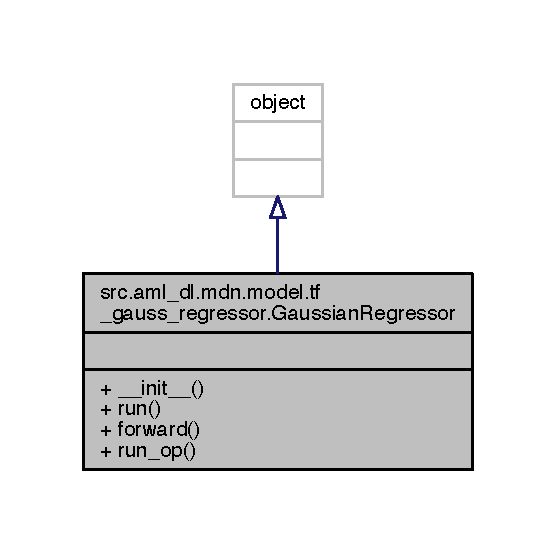
\includegraphics[width=267pt]{classsrc_1_1aml__dl_1_1mdn_1_1model_1_1tf__gauss__regressor_1_1_gaussian_regressor__inherit__graph}
\end{center}
\end{figure}


Collaboration diagram for src.\+aml\+\_\+dl.\+mdn.\+model.\+tf\+\_\+gauss\+\_\+regressor.\+Gaussian\+Regressor\+:
\nopagebreak
\begin{figure}[H]
\begin{center}
\leavevmode
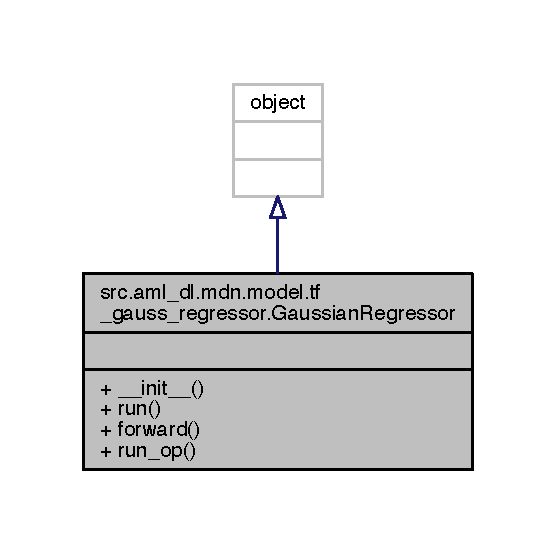
\includegraphics[width=267pt]{classsrc_1_1aml__dl_1_1mdn_1_1model_1_1tf__gauss__regressor_1_1_gaussian_regressor__coll__graph}
\end{center}
\end{figure}
\subsection*{Public Member Functions}
\begin{DoxyCompactItemize}
\item 
\hypertarget{classsrc_1_1aml__dl_1_1mdn_1_1model_1_1tf__gauss__regressor_1_1_gaussian_regressor_a4c80b2988737f5105daa84594d985724}{}\label{classsrc_1_1aml__dl_1_1mdn_1_1model_1_1tf__gauss__regressor_1_1_gaussian_regressor_a4c80b2988737f5105daa84594d985724} 
def {\bfseries \+\_\+\+\_\+init\+\_\+\+\_\+} (self, network\+\_\+params)
\item 
\hypertarget{classsrc_1_1aml__dl_1_1mdn_1_1model_1_1tf__gauss__regressor_1_1_gaussian_regressor_acc12f8257e881010aa7b96fe959456dd}{}\label{classsrc_1_1aml__dl_1_1mdn_1_1model_1_1tf__gauss__regressor_1_1_gaussian_regressor_acc12f8257e881010aa7b96fe959456dd} 
def {\bfseries run} (self, sess, xs, ys=None)
\item 
\hypertarget{classsrc_1_1aml__dl_1_1mdn_1_1model_1_1tf__gauss__regressor_1_1_gaussian_regressor_ae76839400b19f70f2d8c346c536a6264}{}\label{classsrc_1_1aml__dl_1_1mdn_1_1model_1_1tf__gauss__regressor_1_1_gaussian_regressor_ae76839400b19f70f2d8c346c536a6264} 
def {\bfseries forward} (self, sess, xs)
\item 
\hypertarget{classsrc_1_1aml__dl_1_1mdn_1_1model_1_1tf__gauss__regressor_1_1_gaussian_regressor_a93f219ac08506e0c4b51e5c06cd0948b}{}\label{classsrc_1_1aml__dl_1_1mdn_1_1model_1_1tf__gauss__regressor_1_1_gaussian_regressor_a93f219ac08506e0c4b51e5c06cd0948b} 
def {\bfseries run\+\_\+op} (self, sess, op, xs, ys=None)
\end{DoxyCompactItemize}


The documentation for this class was generated from the following file\+:\begin{DoxyCompactItemize}
\item 
aml\+\_\+dl/src/aml\+\_\+dl/mdn/model/tf\+\_\+gauss\+\_\+regressor.\+py\end{DoxyCompactItemize}

\hypertarget{classaml__robot_1_1baxter__ik_1_1_i_k_baxter}{\section{aml\-\_\-robot.\-baxter\-\_\-ik.\-I\-K\-Baxter Class Reference}
\label{classaml__robot_1_1baxter__ik_1_1_i_k_baxter}\index{aml\-\_\-robot.\-baxter\-\_\-ik.\-I\-K\-Baxter@{aml\-\_\-robot.\-baxter\-\_\-ik.\-I\-K\-Baxter}}
}


Collaboration diagram for aml\-\_\-robot.\-baxter\-\_\-ik.\-I\-K\-Baxter\-:\nopagebreak
\begin{figure}[H]
\begin{center}
\leavevmode
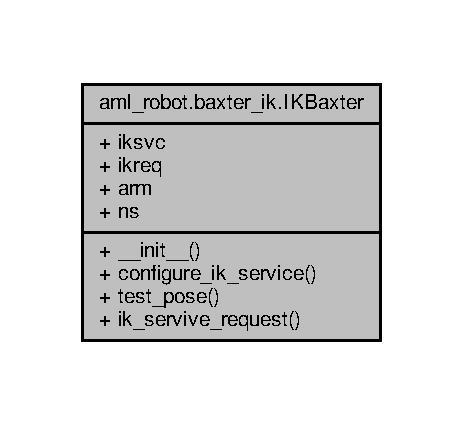
\includegraphics[width=222pt]{classaml__robot_1_1baxter__ik_1_1_i_k_baxter__coll__graph}
\end{center}
\end{figure}
\subsection*{Public Member Functions}
\begin{DoxyCompactItemize}
\item 
\hypertarget{classaml__robot_1_1baxter__ik_1_1_i_k_baxter_acdcbd683c692f89daec2685a9ec2e623}{def {\bfseries \-\_\-\-\_\-init\-\_\-\-\_\-}}\label{classaml__robot_1_1baxter__ik_1_1_i_k_baxter_acdcbd683c692f89daec2685a9ec2e623}

\item 
\hypertarget{classaml__robot_1_1baxter__ik_1_1_i_k_baxter_a6985adef358e80b1924292508a707a66}{def {\bfseries configure\-\_\-ik\-\_\-service}}\label{classaml__robot_1_1baxter__ik_1_1_i_k_baxter_a6985adef358e80b1924292508a707a66}

\item 
\hypertarget{classaml__robot_1_1baxter__ik_1_1_i_k_baxter_a87fb9334e61c8d42b4ff2c5e00402b98}{def {\bfseries test\-\_\-pose}}\label{classaml__robot_1_1baxter__ik_1_1_i_k_baxter_a87fb9334e61c8d42b4ff2c5e00402b98}

\item 
\hypertarget{classaml__robot_1_1baxter__ik_1_1_i_k_baxter_a306f472f1d9fd2105c6d42f092bf476c}{def {\bfseries ik\-\_\-servive\-\_\-request}}\label{classaml__robot_1_1baxter__ik_1_1_i_k_baxter_a306f472f1d9fd2105c6d42f092bf476c}

\end{DoxyCompactItemize}
\subsection*{Public Attributes}
\begin{DoxyCompactItemize}
\item 
\hypertarget{classaml__robot_1_1baxter__ik_1_1_i_k_baxter_a8febd21258f15a3721ecdddd275c9bef}{{\bfseries iksvc}}\label{classaml__robot_1_1baxter__ik_1_1_i_k_baxter_a8febd21258f15a3721ecdddd275c9bef}

\item 
\hypertarget{classaml__robot_1_1baxter__ik_1_1_i_k_baxter_ac3a37bd5bdcafced7d11cff004d5a5da}{{\bfseries ikreq}}\label{classaml__robot_1_1baxter__ik_1_1_i_k_baxter_ac3a37bd5bdcafced7d11cff004d5a5da}

\item 
\hypertarget{classaml__robot_1_1baxter__ik_1_1_i_k_baxter_a31eb6a0623788ecb628c413f6c1cf85a}{{\bfseries arm}}\label{classaml__robot_1_1baxter__ik_1_1_i_k_baxter_a31eb6a0623788ecb628c413f6c1cf85a}

\item 
\hypertarget{classaml__robot_1_1baxter__ik_1_1_i_k_baxter_a006f01e493d58ff9db613d66baa07a63}{{\bfseries ns}}\label{classaml__robot_1_1baxter__ik_1_1_i_k_baxter_a006f01e493d58ff9db613d66baa07a63}

\end{DoxyCompactItemize}


The documentation for this class was generated from the following file\-:\begin{DoxyCompactItemize}
\item 
aml\-\_\-robot/src/aml\-\_\-robot/baxter\-\_\-ik.\-py\end{DoxyCompactItemize}

\hypertarget{classaml__ctrl_1_1controllers_1_1js__controller_1_1_j_s_controller}{\section{aml\-\_\-ctrl.\-controllers.\-js\-\_\-controller.\-J\-S\-Controller Class Reference}
\label{classaml__ctrl_1_1controllers_1_1js__controller_1_1_j_s_controller}\index{aml\-\_\-ctrl.\-controllers.\-js\-\_\-controller.\-J\-S\-Controller@{aml\-\_\-ctrl.\-controllers.\-js\-\_\-controller.\-J\-S\-Controller}}
}


Inheritance diagram for aml\-\_\-ctrl.\-controllers.\-js\-\_\-controller.\-J\-S\-Controller\-:\nopagebreak
\begin{figure}[H]
\begin{center}
\leavevmode
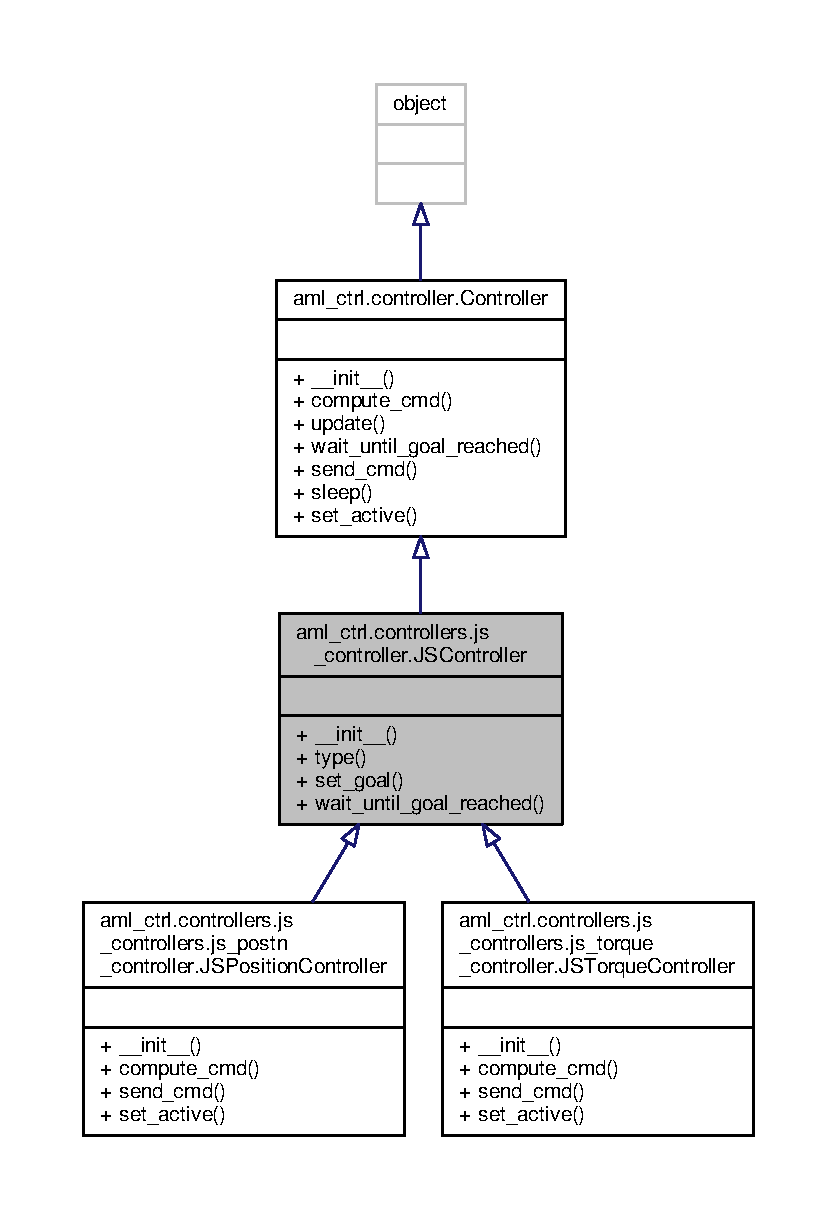
\includegraphics[width=350pt]{classaml__ctrl_1_1controllers_1_1js__controller_1_1_j_s_controller__inherit__graph}
\end{center}
\end{figure}


Collaboration diagram for aml\-\_\-ctrl.\-controllers.\-js\-\_\-controller.\-J\-S\-Controller\-:\nopagebreak
\begin{figure}[H]
\begin{center}
\leavevmode
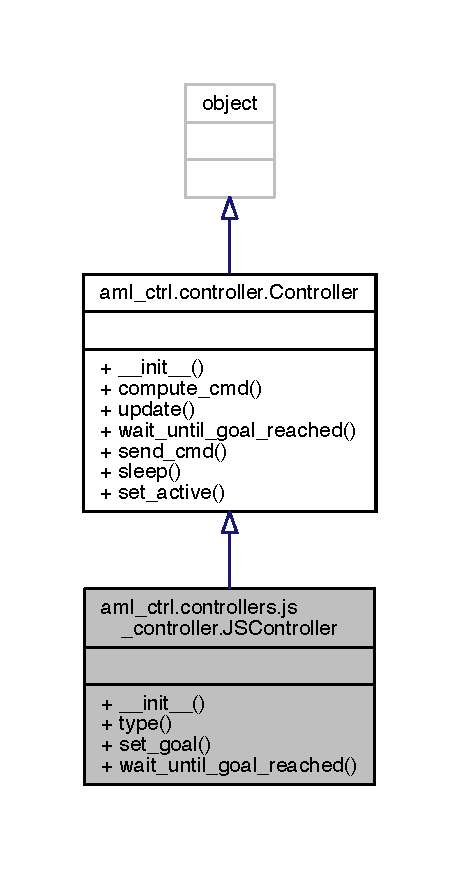
\includegraphics[width=218pt]{classaml__ctrl_1_1controllers_1_1js__controller_1_1_j_s_controller__coll__graph}
\end{center}
\end{figure}
\subsection*{Public Member Functions}
\begin{DoxyCompactItemize}
\item 
\hypertarget{classaml__ctrl_1_1controllers_1_1js__controller_1_1_j_s_controller_a1be5960e312e049110b8991d51210cfe}{def {\bfseries \-\_\-\-\_\-init\-\_\-\-\_\-}}\label{classaml__ctrl_1_1controllers_1_1js__controller_1_1_j_s_controller_a1be5960e312e049110b8991d51210cfe}

\item 
\hypertarget{classaml__ctrl_1_1controllers_1_1js__controller_1_1_j_s_controller_a79e68c4d8dacce86034685b456d73f35}{def {\bfseries type}}\label{classaml__ctrl_1_1controllers_1_1js__controller_1_1_j_s_controller_a79e68c4d8dacce86034685b456d73f35}

\item 
\hypertarget{classaml__ctrl_1_1controllers_1_1js__controller_1_1_j_s_controller_a6fc08eab26adc2e6b8203000c6354995}{def {\bfseries set\-\_\-goal}}\label{classaml__ctrl_1_1controllers_1_1js__controller_1_1_j_s_controller_a6fc08eab26adc2e6b8203000c6354995}

\item 
\hypertarget{classaml__ctrl_1_1controllers_1_1js__controller_1_1_j_s_controller_abe8dc6b50975e05b50c4f7ab2c2caf7c}{def {\bfseries wait\-\_\-until\-\_\-goal\-\_\-reached}}\label{classaml__ctrl_1_1controllers_1_1js__controller_1_1_j_s_controller_abe8dc6b50975e05b50c4f7ab2c2caf7c}

\end{DoxyCompactItemize}


The documentation for this class was generated from the following file\-:\begin{DoxyCompactItemize}
\item 
aml\-\_\-ctrl/src/aml\-\_\-ctrl/controllers/js\-\_\-controller.\-py\end{DoxyCompactItemize}

\hypertarget{classaml__ctrl_1_1controllers_1_1js__controllers_1_1js__postn__controller_1_1_j_s_position_controller}{\section{aml\-\_\-ctrl.\-controllers.\-js\-\_\-controllers.\-js\-\_\-postn\-\_\-controller.\-J\-S\-Position\-Controller Class Reference}
\label{classaml__ctrl_1_1controllers_1_1js__controllers_1_1js__postn__controller_1_1_j_s_position_controller}\index{aml\-\_\-ctrl.\-controllers.\-js\-\_\-controllers.\-js\-\_\-postn\-\_\-controller.\-J\-S\-Position\-Controller@{aml\-\_\-ctrl.\-controllers.\-js\-\_\-controllers.\-js\-\_\-postn\-\_\-controller.\-J\-S\-Position\-Controller}}
}


Inheritance diagram for aml\-\_\-ctrl.\-controllers.\-js\-\_\-controllers.\-js\-\_\-postn\-\_\-controller.\-J\-S\-Position\-Controller\-:
\nopagebreak
\begin{figure}[H]
\begin{center}
\leavevmode
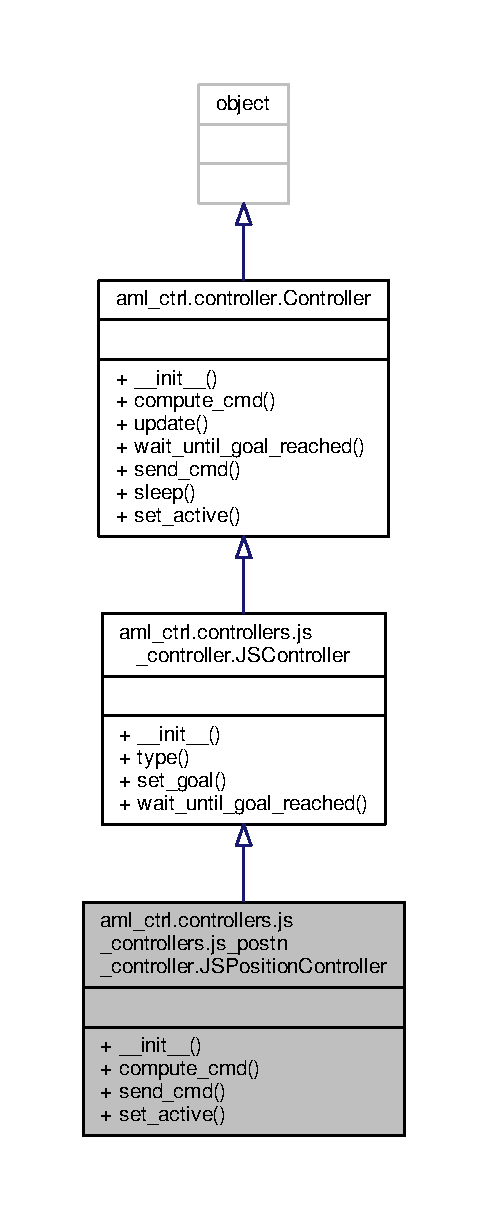
\includegraphics[height=550pt]{classaml__ctrl_1_1controllers_1_1js__controllers_1_1js__postn__controller_1_1_j_s_position_controller__inherit__graph}
\end{center}
\end{figure}


Collaboration diagram for aml\-\_\-ctrl.\-controllers.\-js\-\_\-controllers.\-js\-\_\-postn\-\_\-controller.\-J\-S\-Position\-Controller\-:
\nopagebreak
\begin{figure}[H]
\begin{center}
\leavevmode
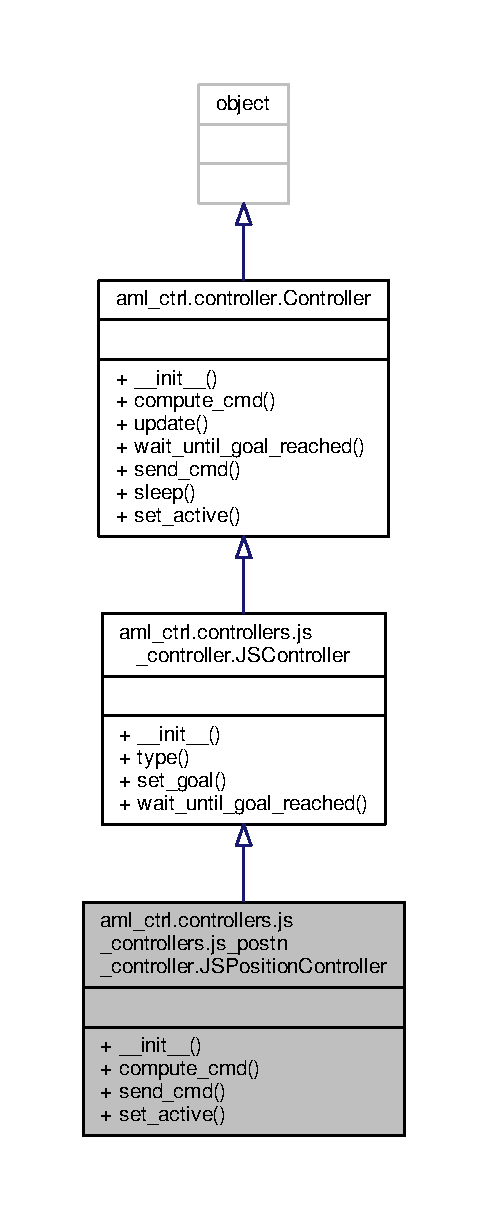
\includegraphics[height=550pt]{classaml__ctrl_1_1controllers_1_1js__controllers_1_1js__postn__controller_1_1_j_s_position_controller__coll__graph}
\end{center}
\end{figure}
\subsection*{Public Member Functions}
\begin{DoxyCompactItemize}
\item 
\hypertarget{classaml__ctrl_1_1controllers_1_1js__controllers_1_1js__postn__controller_1_1_j_s_position_controller_ac463a885a8605d9493b750bb479cb6a8}{def {\bfseries \-\_\-\-\_\-init\-\_\-\-\_\-}}\label{classaml__ctrl_1_1controllers_1_1js__controllers_1_1js__postn__controller_1_1_j_s_position_controller_ac463a885a8605d9493b750bb479cb6a8}

\item 
\hypertarget{classaml__ctrl_1_1controllers_1_1js__controllers_1_1js__postn__controller_1_1_j_s_position_controller_a17033e0eba8bfa1c3a2681089feb7bc4}{def {\bfseries compute\-\_\-cmd}}\label{classaml__ctrl_1_1controllers_1_1js__controllers_1_1js__postn__controller_1_1_j_s_position_controller_a17033e0eba8bfa1c3a2681089feb7bc4}

\item 
\hypertarget{classaml__ctrl_1_1controllers_1_1js__controllers_1_1js__postn__controller_1_1_j_s_position_controller_adff2d8a101823f2830097b24c097d01a}{def {\bfseries send\-\_\-cmd}}\label{classaml__ctrl_1_1controllers_1_1js__controllers_1_1js__postn__controller_1_1_j_s_position_controller_adff2d8a101823f2830097b24c097d01a}

\item 
\hypertarget{classaml__ctrl_1_1controllers_1_1js__controllers_1_1js__postn__controller_1_1_j_s_position_controller_a4748c9f80fbbc3b24326e295d0755482}{def {\bfseries set\-\_\-active}}\label{classaml__ctrl_1_1controllers_1_1js__controllers_1_1js__postn__controller_1_1_j_s_position_controller_a4748c9f80fbbc3b24326e295d0755482}

\end{DoxyCompactItemize}


The documentation for this class was generated from the following file\-:\begin{DoxyCompactItemize}
\item 
aml\-\_\-ctrl/src/aml\-\_\-ctrl/controllers/js\-\_\-controllers/js\-\_\-postn\-\_\-controller.\-py\end{DoxyCompactItemize}

\hypertarget{classaml__ctrl_1_1controllers_1_1js__controllers_1_1js__torque__controller_1_1_j_s_torque_controller}{}\section{aml\+\_\+ctrl.\+controllers.\+js\+\_\+controllers.\+js\+\_\+torque\+\_\+controller.\+J\+S\+Torque\+Controller Class Reference}
\label{classaml__ctrl_1_1controllers_1_1js__controllers_1_1js__torque__controller_1_1_j_s_torque_controller}\index{aml\+\_\+ctrl.\+controllers.\+js\+\_\+controllers.\+js\+\_\+torque\+\_\+controller.\+J\+S\+Torque\+Controller@{aml\+\_\+ctrl.\+controllers.\+js\+\_\+controllers.\+js\+\_\+torque\+\_\+controller.\+J\+S\+Torque\+Controller}}


Inheritance diagram for aml\+\_\+ctrl.\+controllers.\+js\+\_\+controllers.\+js\+\_\+torque\+\_\+controller.\+J\+S\+Torque\+Controller\+:\nopagebreak
\begin{figure}[H]
\begin{center}
\leavevmode
\includegraphics[height=550pt]{classaml__ctrl_1_1controllers_1_1js__controllers_1_1js__torque__controller_1_1_j_s_torque_controller__inherit__graph}
\end{center}
\end{figure}


Collaboration diagram for aml\+\_\+ctrl.\+controllers.\+js\+\_\+controllers.\+js\+\_\+torque\+\_\+controller.\+J\+S\+Torque\+Controller\+:\nopagebreak
\begin{figure}[H]
\begin{center}
\leavevmode
\includegraphics[height=550pt]{classaml__ctrl_1_1controllers_1_1js__controllers_1_1js__torque__controller_1_1_j_s_torque_controller__coll__graph}
\end{center}
\end{figure}
\subsection*{Public Member Functions}
\begin{DoxyCompactItemize}
\item 
\hypertarget{classaml__ctrl_1_1controllers_1_1js__controllers_1_1js__torque__controller_1_1_j_s_torque_controller_a6c4438a0f7de1511e34fff8dd78f6999}{}\label{classaml__ctrl_1_1controllers_1_1js__controllers_1_1js__torque__controller_1_1_j_s_torque_controller_a6c4438a0f7de1511e34fff8dd78f6999} 
def {\bfseries \+\_\+\+\_\+init\+\_\+\+\_\+} (self, robot\+\_\+interface, config=J\+S\+\_\+\+T\+O\+R\+Q\+U\+E\+\_\+\+C\+N\+T\+LR)
\item 
\hypertarget{classaml__ctrl_1_1controllers_1_1js__controllers_1_1js__torque__controller_1_1_j_s_torque_controller_a1f6cfa660a0b6e9f123c544bac73a8b2}{}\label{classaml__ctrl_1_1controllers_1_1js__controllers_1_1js__torque__controller_1_1_j_s_torque_controller_a1f6cfa660a0b6e9f123c544bac73a8b2} 
def {\bfseries compute\+\_\+cmd} (self, time\+\_\+elapsed)
\item 
\hypertarget{classaml__ctrl_1_1controllers_1_1js__controllers_1_1js__torque__controller_1_1_j_s_torque_controller_a339d1c5d2acc1859605f5c87200a88bf}{}\label{classaml__ctrl_1_1controllers_1_1js__controllers_1_1js__torque__controller_1_1_j_s_torque_controller_a339d1c5d2acc1859605f5c87200a88bf} 
def {\bfseries send\+\_\+cmd} (self, time\+\_\+elapsed)
\item 
\hypertarget{classaml__ctrl_1_1controllers_1_1js__controllers_1_1js__torque__controller_1_1_j_s_torque_controller_ad422e4ee2a27feaa48be0d483ab3132d}{}\label{classaml__ctrl_1_1controllers_1_1js__controllers_1_1js__torque__controller_1_1_j_s_torque_controller_ad422e4ee2a27feaa48be0d483ab3132d} 
def {\bfseries set\+\_\+active} (self, is\+\_\+active)
\end{DoxyCompactItemize}


The documentation for this class was generated from the following file\+:\begin{DoxyCompactItemize}
\item 
aml\+\_\+ctrl/src/aml\+\_\+ctrl/controllers/js\+\_\+controllers/js\+\_\+torque\+\_\+controller.\+py\end{DoxyCompactItemize}

\hypertarget{classaml__ctrl_1_1traj__generator_1_1js__traj__generator_1_1_j_s_traj_generator}{}\section{aml\+\_\+ctrl.\+traj\+\_\+generator.\+js\+\_\+traj\+\_\+generator.\+J\+S\+Traj\+Generator Class Reference}
\label{classaml__ctrl_1_1traj__generator_1_1js__traj__generator_1_1_j_s_traj_generator}\index{aml\+\_\+ctrl.\+traj\+\_\+generator.\+js\+\_\+traj\+\_\+generator.\+J\+S\+Traj\+Generator@{aml\+\_\+ctrl.\+traj\+\_\+generator.\+js\+\_\+traj\+\_\+generator.\+J\+S\+Traj\+Generator}}


Inheritance diagram for aml\+\_\+ctrl.\+traj\+\_\+generator.\+js\+\_\+traj\+\_\+generator.\+J\+S\+Traj\+Generator\+:\nopagebreak
\begin{figure}[H]
\begin{center}
\leavevmode
\includegraphics[width=240pt]{classaml__ctrl_1_1traj__generator_1_1js__traj__generator_1_1_j_s_traj_generator__inherit__graph}
\end{center}
\end{figure}


Collaboration diagram for aml\+\_\+ctrl.\+traj\+\_\+generator.\+js\+\_\+traj\+\_\+generator.\+J\+S\+Traj\+Generator\+:\nopagebreak
\begin{figure}[H]
\begin{center}
\leavevmode
\includegraphics[width=240pt]{classaml__ctrl_1_1traj__generator_1_1js__traj__generator_1_1_j_s_traj_generator__coll__graph}
\end{center}
\end{figure}
\subsection*{Public Member Functions}
\begin{DoxyCompactItemize}
\item 
\hypertarget{classaml__ctrl_1_1traj__generator_1_1js__traj__generator_1_1_j_s_traj_generator_a8f3f80b67d5c1ca0821cd311764636ec}{}\label{classaml__ctrl_1_1traj__generator_1_1js__traj__generator_1_1_j_s_traj_generator_a8f3f80b67d5c1ca0821cd311764636ec} 
def {\bfseries \+\_\+\+\_\+init\+\_\+\+\_\+} (self, load\+\_\+from\+\_\+demo=False, kwargs)
\item 
\hypertarget{classaml__ctrl_1_1traj__generator_1_1js__traj__generator_1_1_j_s_traj_generator_a022b44a0ef727669bb5c5a12b6ed9b44}{}\label{classaml__ctrl_1_1traj__generator_1_1js__traj__generator_1_1_j_s_traj_generator_a022b44a0ef727669bb5c5a12b6ed9b44} 
def {\bfseries configure} (self, robot\+\_\+interface)
\item 
\hypertarget{classaml__ctrl_1_1traj__generator_1_1js__traj__generator_1_1_j_s_traj_generator_ad5f065b319964c3e6640c700eabf2361}{}\label{classaml__ctrl_1_1traj__generator_1_1js__traj__generator_1_1_j_s_traj_generator_ad5f065b319964c3e6640c700eabf2361} 
def {\bfseries get\+\_\+demo\+\_\+traj} (self)
\item 
\hypertarget{classaml__ctrl_1_1traj__generator_1_1js__traj__generator_1_1_j_s_traj_generator_a8844409ef5da594ac029efbb4c60f617}{}\label{classaml__ctrl_1_1traj__generator_1_1js__traj__generator_1_1_j_s_traj_generator_a8844409ef5da594ac029efbb4c60f617} 
def {\bfseries get\+\_\+traj\+\_\+interp} (self)
\item 
\hypertarget{classaml__ctrl_1_1traj__generator_1_1js__traj__generator_1_1_j_s_traj_generator_a8aeb635dc050800d6dad4a7f34d32f26}{}\label{classaml__ctrl_1_1traj__generator_1_1js__traj__generator_1_1_j_s_traj_generator_a8aeb635dc050800d6dad4a7f34d32f26} 
def {\bfseries convert\+\_\+os\+\_\+to\+\_\+js} (self, os\+\_\+traj=None)
\item 
\hypertarget{classaml__ctrl_1_1traj__generator_1_1js__traj__generator_1_1_j_s_traj_generator_a449ff9de50f0939e27a5ae11e9c4cfb0}{}\label{classaml__ctrl_1_1traj__generator_1_1js__traj__generator_1_1_j_s_traj_generator_a449ff9de50f0939e27a5ae11e9c4cfb0} 
def {\bfseries generate\+\_\+traj} (self)
\end{DoxyCompactItemize}


The documentation for this class was generated from the following file\+:\begin{DoxyCompactItemize}
\item 
aml\+\_\+ctrl/src/aml\+\_\+ctrl/traj\+\_\+generator/js\+\_\+traj\+\_\+generator.\+py\end{DoxyCompactItemize}

\hypertarget{classaml__lfd_1_1lfd_1_1_lf_d}{\section{aml\-\_\-lfd.\-lfd.\-Lf\-D Class Reference}
\label{classaml__lfd_1_1lfd_1_1_lf_d}\index{aml\-\_\-lfd.\-lfd.\-Lf\-D@{aml\-\_\-lfd.\-lfd.\-Lf\-D}}
}


Inheritance diagram for aml\-\_\-lfd.\-lfd.\-Lf\-D\-:\nopagebreak
\begin{figure}[H]
\begin{center}
\leavevmode
\includegraphics[width=172pt]{classaml__lfd_1_1lfd_1_1_lf_d__inherit__graph}
\end{center}
\end{figure}


Collaboration diagram for aml\-\_\-lfd.\-lfd.\-Lf\-D\-:\nopagebreak
\begin{figure}[H]
\begin{center}
\leavevmode
\includegraphics[width=172pt]{classaml__lfd_1_1lfd_1_1_lf_d__coll__graph}
\end{center}
\end{figure}
\subsection*{Public Member Functions}
\begin{DoxyCompactItemize}
\item 
\hypertarget{classaml__lfd_1_1lfd_1_1_lf_d_aab9046d6d3824e7bfeea0eddbfe5054f}{def {\bfseries \-\_\-\-\_\-init\-\_\-\-\_\-}}\label{classaml__lfd_1_1lfd_1_1_lf_d_aab9046d6d3824e7bfeea0eddbfe5054f}

\item 
\hypertarget{classaml__lfd_1_1lfd_1_1_lf_d_a0f3dff0ab9b2d70047d3a2679cd5152e}{def {\bfseries encode\-\_\-demo}}\label{classaml__lfd_1_1lfd_1_1_lf_d_a0f3dff0ab9b2d70047d3a2679cd5152e}

\end{DoxyCompactItemize}


The documentation for this class was generated from the following file\-:\begin{DoxyCompactItemize}
\item 
aml\-\_\-lfd/src/aml\-\_\-lfd/lfd.\-py\end{DoxyCompactItemize}

\hypertarget{classaml__ctrl_1_1utilities_1_1lin__interp_1_1_lin_interp}{\section{aml\-\_\-ctrl.\-utilities.\-lin\-\_\-interp.\-Lin\-Interp Class Reference}
\label{classaml__ctrl_1_1utilities_1_1lin__interp_1_1_lin_interp}\index{aml\-\_\-ctrl.\-utilities.\-lin\-\_\-interp.\-Lin\-Interp@{aml\-\_\-ctrl.\-utilities.\-lin\-\_\-interp.\-Lin\-Interp}}
}


Collaboration diagram for aml\-\_\-ctrl.\-utilities.\-lin\-\_\-interp.\-Lin\-Interp\-:
\nopagebreak
\begin{figure}[H]
\begin{center}
\leavevmode
\includegraphics[width=226pt]{classaml__ctrl_1_1utilities_1_1lin__interp_1_1_lin_interp__coll__graph}
\end{center}
\end{figure}
\subsection*{Public Member Functions}
\begin{DoxyCompactItemize}
\item 
\hypertarget{classaml__ctrl_1_1utilities_1_1lin__interp_1_1_lin_interp_a1e35790a94c93ae7d3d8024028c550ff}{def {\bfseries \-\_\-\-\_\-init\-\_\-\-\_\-}}\label{classaml__ctrl_1_1utilities_1_1lin__interp_1_1_lin_interp_a1e35790a94c93ae7d3d8024028c550ff}

\item 
\hypertarget{classaml__ctrl_1_1utilities_1_1lin__interp_1_1_lin_interp_a14a7de9dcf847e85448a5e5b1d061e94}{def {\bfseries configure}}\label{classaml__ctrl_1_1utilities_1_1lin__interp_1_1_lin_interp_a14a7de9dcf847e85448a5e5b1d061e94}

\item 
\hypertarget{classaml__ctrl_1_1utilities_1_1lin__interp_1_1_lin_interp_a4ed2ce1b4e7cc2b115247fb09a7847ad}{def {\bfseries lin\-\_\-step\-\_\-qt}}\label{classaml__ctrl_1_1utilities_1_1lin__interp_1_1_lin_interp_a4ed2ce1b4e7cc2b115247fb09a7847ad}

\item 
\hypertarget{classaml__ctrl_1_1utilities_1_1lin__interp_1_1_lin_interp_a4938f92638c8384e71cbdc9ca57fd0e0}{def {\bfseries lin\-\_\-step\-\_\-pos}}\label{classaml__ctrl_1_1utilities_1_1lin__interp_1_1_lin_interp_a4938f92638c8384e71cbdc9ca57fd0e0}

\item 
\hypertarget{classaml__ctrl_1_1utilities_1_1lin__interp_1_1_lin_interp_a50602f7c9cfa8746de0fda436e6b6283}{def {\bfseries get\-\_\-interpolated\-\_\-trajectory}}\label{classaml__ctrl_1_1utilities_1_1lin__interp_1_1_lin_interp_a50602f7c9cfa8746de0fda436e6b6283}

\item 
\hypertarget{classaml__ctrl_1_1utilities_1_1lin__interp_1_1_lin_interp_ab08c5f7742c601b1523f7d82216e2f3e}{def {\bfseries plot\-\_\-lin\-\_\-interp\-\_\-traj}}\label{classaml__ctrl_1_1utilities_1_1lin__interp_1_1_lin_interp_ab08c5f7742c601b1523f7d82216e2f3e}

\end{DoxyCompactItemize}
\subsection*{Public Attributes}
\begin{DoxyCompactItemize}
\item 
\hypertarget{classaml__ctrl_1_1utilities_1_1lin__interp_1_1_lin_interp_a91ce8d62c538477b2e4e30cc604b9d60}{{\bfseries dt}}\label{classaml__ctrl_1_1utilities_1_1lin__interp_1_1_lin_interp_a91ce8d62c538477b2e4e30cc604b9d60}

\item 
\hypertarget{classaml__ctrl_1_1utilities_1_1lin__interp_1_1_lin_interp_a3a9296ff1896b9de1f43ebf138554658}{{\bfseries tau}}\label{classaml__ctrl_1_1utilities_1_1lin__interp_1_1_lin_interp_a3a9296ff1896b9de1f43ebf138554658}

\item 
\hypertarget{classaml__ctrl_1_1utilities_1_1lin__interp_1_1_lin_interp_a601fd091f2e367969d20dced930e84ca}{{\bfseries timesteps}}\label{classaml__ctrl_1_1utilities_1_1lin__interp_1_1_lin_interp_a601fd091f2e367969d20dced930e84ca}

\item 
\hypertarget{classaml__ctrl_1_1utilities_1_1lin__interp_1_1_lin_interp_a636787254c4170344140b25b54139782}{{\bfseries lin\-\_\-interp\-\_\-traj}}\label{classaml__ctrl_1_1utilities_1_1lin__interp_1_1_lin_interp_a636787254c4170344140b25b54139782}

\item 
\hypertarget{classaml__ctrl_1_1utilities_1_1lin__interp_1_1_lin_interp_af6583e2f56c7732af967927541ed01ce}{{\bfseries start\-\_\-pos}}\label{classaml__ctrl_1_1utilities_1_1lin__interp_1_1_lin_interp_af6583e2f56c7732af967927541ed01ce}

\item 
\hypertarget{classaml__ctrl_1_1utilities_1_1lin__interp_1_1_lin_interp_a2827d5e7e445519eb94643982b8fbe15}{{\bfseries goal\-\_\-pos}}\label{classaml__ctrl_1_1utilities_1_1lin__interp_1_1_lin_interp_a2827d5e7e445519eb94643982b8fbe15}

\item 
\hypertarget{classaml__ctrl_1_1utilities_1_1lin__interp_1_1_lin_interp_a8e59d6ea4a99b6ef7ed6a8acaac632d4}{{\bfseries start\-\_\-qt}}\label{classaml__ctrl_1_1utilities_1_1lin__interp_1_1_lin_interp_a8e59d6ea4a99b6ef7ed6a8acaac632d4}

\item 
\hypertarget{classaml__ctrl_1_1utilities_1_1lin__interp_1_1_lin_interp_ac042c31929df9c729e392ee7bc72a84a}{{\bfseries goal\-\_\-qt}}\label{classaml__ctrl_1_1utilities_1_1lin__interp_1_1_lin_interp_ac042c31929df9c729e392ee7bc72a84a}

\end{DoxyCompactItemize}


The documentation for this class was generated from the following file\-:\begin{DoxyCompactItemize}
\item 
aml\-\_\-ctrl/src/aml\-\_\-ctrl/utilities/lin\-\_\-interp.\-py\end{DoxyCompactItemize}

\hypertarget{classsrc_1_1aml__dl_1_1mdn_1_1utilities_1_1get__pre__process__data_1_1_load_preprocess_data}{\section{src.\-aml\-\_\-dl.\-mdn.\-utilities.\-get\-\_\-pre\-\_\-process\-\_\-data.\-Load\-Preprocess\-Data Class Reference}
\label{classsrc_1_1aml__dl_1_1mdn_1_1utilities_1_1get__pre__process__data_1_1_load_preprocess_data}\index{src.\-aml\-\_\-dl.\-mdn.\-utilities.\-get\-\_\-pre\-\_\-process\-\_\-data.\-Load\-Preprocess\-Data@{src.\-aml\-\_\-dl.\-mdn.\-utilities.\-get\-\_\-pre\-\_\-process\-\_\-data.\-Load\-Preprocess\-Data}}
}


Collaboration diagram for src.\-aml\-\_\-dl.\-mdn.\-utilities.\-get\-\_\-pre\-\_\-process\-\_\-data.\-Load\-Preprocess\-Data\-:
\nopagebreak
\begin{figure}[H]
\begin{center}
\leavevmode
\includegraphics[width=272pt]{classsrc_1_1aml__dl_1_1mdn_1_1utilities_1_1get__pre__process__data_1_1_load_preprocess_data__coll__graph}
\end{center}
\end{figure}
\subsection*{Public Member Functions}
\begin{DoxyCompactItemize}
\item 
\hypertarget{classsrc_1_1aml__dl_1_1mdn_1_1utilities_1_1get__pre__process__data_1_1_load_preprocess_data_a8a19efbe586a07ceb103b9f393aa96e0}{def {\bfseries \-\_\-\-\_\-init\-\_\-\-\_\-}}\label{classsrc_1_1aml__dl_1_1mdn_1_1utilities_1_1get__pre__process__data_1_1_load_preprocess_data_a8a19efbe586a07ceb103b9f393aa96e0}

\item 
\hypertarget{classsrc_1_1aml__dl_1_1mdn_1_1utilities_1_1get__pre__process__data_1_1_load_preprocess_data_a3845622f8dffba8f59b154540f70c74d}{def {\bfseries get\-\_\-file\-\_\-names}}\label{classsrc_1_1aml__dl_1_1mdn_1_1utilities_1_1get__pre__process__data_1_1_load_preprocess_data_a3845622f8dffba8f59b154540f70c74d}

\item 
\hypertarget{classsrc_1_1aml__dl_1_1mdn_1_1utilities_1_1get__pre__process__data_1_1_load_preprocess_data_add4e5d98ff7c6dcf58e3ee766348949a}{def {\bfseries update\-\_\-file\-\_\-idx}}\label{classsrc_1_1aml__dl_1_1mdn_1_1utilities_1_1get__pre__process__data_1_1_load_preprocess_data_add4e5d98ff7c6dcf58e3ee766348949a}

\item 
\hypertarget{classsrc_1_1aml__dl_1_1mdn_1_1utilities_1_1get__pre__process__data_1_1_load_preprocess_data_afc7d5d2e1a5f2cfd71efc07d35195802}{def {\bfseries load\-\_\-data}}\label{classsrc_1_1aml__dl_1_1mdn_1_1utilities_1_1get__pre__process__data_1_1_load_preprocess_data_afc7d5d2e1a5f2cfd71efc07d35195802}

\end{DoxyCompactItemize}


The documentation for this class was generated from the following file\-:\begin{DoxyCompactItemize}
\item 
aml\-\_\-dl/src/aml\-\_\-dl/mdn/utilities/get\-\_\-pre\-\_\-process\-\_\-data.\-py\end{DoxyCompactItemize}

\hypertarget{classaml__lfd_1_1lqr_1_1lqr__traj__follow_1_1_l_q_r_traj_follow}{\section{aml\-\_\-lfd.\-lqr.\-lqr\-\_\-traj\-\_\-follow.\-L\-Q\-R\-Traj\-Follow Class Reference}
\label{classaml__lfd_1_1lqr_1_1lqr__traj__follow_1_1_l_q_r_traj_follow}\index{aml\-\_\-lfd.\-lqr.\-lqr\-\_\-traj\-\_\-follow.\-L\-Q\-R\-Traj\-Follow@{aml\-\_\-lfd.\-lqr.\-lqr\-\_\-traj\-\_\-follow.\-L\-Q\-R\-Traj\-Follow}}
}


Collaboration diagram for aml\-\_\-lfd.\-lqr.\-lqr\-\_\-traj\-\_\-follow.\-L\-Q\-R\-Traj\-Follow\-:
\nopagebreak
\begin{figure}[H]
\begin{center}
\leavevmode
\includegraphics[width=200pt]{classaml__lfd_1_1lqr_1_1lqr__traj__follow_1_1_l_q_r_traj_follow__coll__graph}
\end{center}
\end{figure}
\subsection*{Public Member Functions}
\begin{DoxyCompactItemize}
\item 
\hypertarget{classaml__lfd_1_1lqr_1_1lqr__traj__follow_1_1_l_q_r_traj_follow_acbb05476cbb16e8e238eaecc375bd062}{def {\bfseries \-\_\-\-\_\-init\-\_\-\-\_\-}}\label{classaml__lfd_1_1lqr_1_1lqr__traj__follow_1_1_l_q_r_traj_follow_acbb05476cbb16e8e238eaecc375bd062}

\item 
\hypertarget{classaml__lfd_1_1lqr_1_1lqr__traj__follow_1_1_l_q_r_traj_follow_ac4e443bc2b3b58dfb909dd1084a11a11}{def {\bfseries configure}}\label{classaml__lfd_1_1lqr_1_1lqr__traj__follow_1_1_l_q_r_traj_follow_ac4e443bc2b3b58dfb909dd1084a11a11}

\item 
\hypertarget{classaml__lfd_1_1lqr_1_1lqr__traj__follow_1_1_l_q_r_traj_follow_a36a88a75e595f13d0b6717f35fa5ab91}{def {\bfseries compute\-\_\-dx}}\label{classaml__lfd_1_1lqr_1_1lqr__traj__follow_1_1_l_q_r_traj_follow_a36a88a75e595f13d0b6717f35fa5ab91}

\item 
\hypertarget{classaml__lfd_1_1lqr_1_1lqr__traj__follow_1_1_l_q_r_traj_follow_a7fd528502e2e6f355dd0a78e85edbde0}{def {\bfseries err\-\_\-simulate}}\label{classaml__lfd_1_1lqr_1_1lqr__traj__follow_1_1_l_q_r_traj_follow_a7fd528502e2e6f355dd0a78e85edbde0}

\item 
\hypertarget{classaml__lfd_1_1lqr_1_1lqr__traj__follow_1_1_l_q_r_traj_follow_a92582e75cb2c7fb600ccf28d0eead6e9}{def {\bfseries compose\-\_\-dx}}\label{classaml__lfd_1_1lqr_1_1lqr__traj__follow_1_1_l_q_r_traj_follow_a92582e75cb2c7fb600ccf28d0eead6e9}

\item 
\hypertarget{classaml__lfd_1_1lqr_1_1lqr__traj__follow_1_1_l_q_r_traj_follow_ae44942a2b3f38265f5864e112e713a4e}{def {\bfseries simulate\-\_\-f}}\label{classaml__lfd_1_1lqr_1_1lqr__traj__follow_1_1_l_q_r_traj_follow_ae44942a2b3f38265f5864e112e713a4e}

\item 
\hypertarget{classaml__lfd_1_1lqr_1_1lqr__traj__follow_1_1_l_q_r_traj_follow_a2b582169fbc023aeb0121fea485cc0ff}{def {\bfseries linearized\-\_\-dynamics}}\label{classaml__lfd_1_1lqr_1_1lqr__traj__follow_1_1_l_q_r_traj_follow_a2b582169fbc023aeb0121fea485cc0ff}

\item 
\hypertarget{classaml__lfd_1_1lqr_1_1lqr__traj__follow_1_1_l_q_r_traj_follow_a690d75d9e9512c773502199444480685}{def {\bfseries lqr}}\label{classaml__lfd_1_1lqr_1_1lqr__traj__follow_1_1_l_q_r_traj_follow_a690d75d9e9512c773502199444480685}

\item 
\hypertarget{classaml__lfd_1_1lqr_1_1lqr__traj__follow_1_1_l_q_r_traj_follow_aa05b359efc9d1779ae81ca0dd3525467}{def {\bfseries dlqr}}\label{classaml__lfd_1_1lqr_1_1lqr__traj__follow_1_1_l_q_r_traj_follow_aa05b359efc9d1779ae81ca0dd3525467}

\item 
\hypertarget{classaml__lfd_1_1lqr_1_1lqr__traj__follow_1_1_l_q_r_traj_follow_adec42df243dc0661ce780b509a714876}{def {\bfseries find\-\_\-feedback\-\_\-gains}}\label{classaml__lfd_1_1lqr_1_1lqr__traj__follow_1_1_l_q_r_traj_follow_adec42df243dc0661ce780b509a714876}

\end{DoxyCompactItemize}
\subsection*{Public Attributes}
\begin{DoxyCompactItemize}
\item 
\hypertarget{classaml__lfd_1_1lqr_1_1lqr__traj__follow_1_1_l_q_r_traj_follow_acdfe028943c87b025cf7fbc06ef70fd0}{{\bfseries idx}}\label{classaml__lfd_1_1lqr_1_1lqr__traj__follow_1_1_l_q_r_traj_follow_acdfe028943c87b025cf7fbc06ef70fd0}

\item 
\hypertarget{classaml__lfd_1_1lqr_1_1lqr__traj__follow_1_1_l_q_r_traj_follow_ab761a4111b05cec415c4a3216084f77d}{{\bfseries H}}\label{classaml__lfd_1_1lqr_1_1lqr__traj__follow_1_1_l_q_r_traj_follow_ab761a4111b05cec415c4a3216084f77d}

\item 
\hypertarget{classaml__lfd_1_1lqr_1_1lqr__traj__follow_1_1_l_q_r_traj_follow_a8f217f0b7f45e88af0249baffe6b9e24}{{\bfseries target\-\_\-traj}}\label{classaml__lfd_1_1lqr_1_1lqr__traj__follow_1_1_l_q_r_traj_follow_a8f217f0b7f45e88af0249baffe6b9e24}

\item 
\hypertarget{classaml__lfd_1_1lqr_1_1lqr__traj__follow_1_1_l_q_r_traj_follow_a5a99d1280c2ca955b078734bc923453d}{{\bfseries model}}\label{classaml__lfd_1_1lqr_1_1lqr__traj__follow_1_1_l_q_r_traj_follow_a5a99d1280c2ca955b078734bc923453d}

\item 
\hypertarget{classaml__lfd_1_1lqr_1_1lqr__traj__follow_1_1_l_q_r_traj_follow_ae74ea09c332230dd2d3a7ea018d2b4f0}{{\bfseries reward}}\label{classaml__lfd_1_1lqr_1_1lqr__traj__follow_1_1_l_q_r_traj_follow_ae74ea09c332230dd2d3a7ea018d2b4f0}

\item 
\hypertarget{classaml__lfd_1_1lqr_1_1lqr__traj__follow_1_1_l_q_r_traj_follow_a90c1612252d53e6cc2c748efd08cc144}{{\bfseries num\-\_\-states}}\label{classaml__lfd_1_1lqr_1_1lqr__traj__follow_1_1_l_q_r_traj_follow_a90c1612252d53e6cc2c748efd08cc144}

\item 
\hypertarget{classaml__lfd_1_1lqr_1_1lqr__traj__follow_1_1_l_q_r_traj_follow_a7636aa71830621dfc55a820451f06c69}{{\bfseries num\-\_\-ctrls}}\label{classaml__lfd_1_1lqr_1_1lqr__traj__follow_1_1_l_q_r_traj_follow_a7636aa71830621dfc55a820451f06c69}

\item 
\hypertarget{classaml__lfd_1_1lqr_1_1lqr__traj__follow_1_1_l_q_r_traj_follow_a7de94731c6015deb36958adbc45b50b3}{{\bfseries num\-\_\-links}}\label{classaml__lfd_1_1lqr_1_1lqr__traj__follow_1_1_l_q_r_traj_follow_a7de94731c6015deb36958adbc45b50b3}

\item 
\hypertarget{classaml__lfd_1_1lqr_1_1lqr__traj__follow_1_1_l_q_r_traj_follow_a5a5623456a1a207a4b61e40ef3f9bac7}{{\bfseries robot}}\label{classaml__lfd_1_1lqr_1_1lqr__traj__follow_1_1_l_q_r_traj_follow_a5a5623456a1a207a4b61e40ef3f9bac7}

\item 
\hypertarget{classaml__lfd_1_1lqr_1_1lqr__traj__follow_1_1_l_q_r_traj_follow_a7ded951bc3a6aa453117ef453cf81d89}{{\bfseries A}}\label{classaml__lfd_1_1lqr_1_1lqr__traj__follow_1_1_l_q_r_traj_follow_a7ded951bc3a6aa453117ef453cf81d89}

\item 
\hypertarget{classaml__lfd_1_1lqr_1_1lqr__traj__follow_1_1_l_q_r_traj_follow_acdc87fa664772ed3a9249d6409b0ffe9}{{\bfseries B}}\label{classaml__lfd_1_1lqr_1_1lqr__traj__follow_1_1_l_q_r_traj_follow_acdc87fa664772ed3a9249d6409b0ffe9}

\item 
\hypertarget{classaml__lfd_1_1lqr_1_1lqr__traj__follow_1_1_l_q_r_traj_follow_a39a7fada44bbd9d99d11833570dd68a4}{{\bfseries Q}}\label{classaml__lfd_1_1lqr_1_1lqr__traj__follow_1_1_l_q_r_traj_follow_a39a7fada44bbd9d99d11833570dd68a4}

\item 
\hypertarget{classaml__lfd_1_1lqr_1_1lqr__traj__follow_1_1_l_q_r_traj_follow_ab0c18118be7bbbef6a6d016418cdbab1}{{\bfseries Qf}}\label{classaml__lfd_1_1lqr_1_1lqr__traj__follow_1_1_l_q_r_traj_follow_ab0c18118be7bbbef6a6d016418cdbab1}

\item 
\hypertarget{classaml__lfd_1_1lqr_1_1lqr__traj__follow_1_1_l_q_r_traj_follow_a7191995bec2a33ced77e96614dcdfef3}{{\bfseries R}}\label{classaml__lfd_1_1lqr_1_1lqr__traj__follow_1_1_l_q_r_traj_follow_a7191995bec2a33ced77e96614dcdfef3}

\item 
\hypertarget{classaml__lfd_1_1lqr_1_1lqr__traj__follow_1_1_l_q_r_traj_follow_a2f8f716d9c1d04fbf3696b41608431d8}{{\bfseries Rf}}\label{classaml__lfd_1_1lqr_1_1lqr__traj__follow_1_1_l_q_r_traj_follow_a2f8f716d9c1d04fbf3696b41608431d8}

\item 
\hypertarget{classaml__lfd_1_1lqr_1_1lqr__traj__follow_1_1_l_q_r_traj_follow_ada7ee9aef1116f1ba812b16a5d007e2c}{{\bfseries Alist}}\label{classaml__lfd_1_1lqr_1_1lqr__traj__follow_1_1_l_q_r_traj_follow_ada7ee9aef1116f1ba812b16a5d007e2c}

\item 
\hypertarget{classaml__lfd_1_1lqr_1_1lqr__traj__follow_1_1_l_q_r_traj_follow_ad99234f85e754237f6b9981fca8ec1db}{{\bfseries Blist}}\label{classaml__lfd_1_1lqr_1_1lqr__traj__follow_1_1_l_q_r_traj_follow_ad99234f85e754237f6b9981fca8ec1db}

\item 
\hypertarget{classaml__lfd_1_1lqr_1_1lqr__traj__follow_1_1_l_q_r_traj_follow_a3f5c63feb46c1c5f53a7654930405866}{{\bfseries Qlist}}\label{classaml__lfd_1_1lqr_1_1lqr__traj__follow_1_1_l_q_r_traj_follow_a3f5c63feb46c1c5f53a7654930405866}

\item 
\hypertarget{classaml__lfd_1_1lqr_1_1lqr__traj__follow_1_1_l_q_r_traj_follow_a677cefc87aae3e07521793209eb6a23d}{{\bfseries Rlist}}\label{classaml__lfd_1_1lqr_1_1lqr__traj__follow_1_1_l_q_r_traj_follow_a677cefc87aae3e07521793209eb6a23d}

\item 
\hypertarget{classaml__lfd_1_1lqr_1_1lqr__traj__follow_1_1_l_q_r_traj_follow_a5f2bda5589414211230b627c8e3a898c}{{\bfseries Klist}}\label{classaml__lfd_1_1lqr_1_1lqr__traj__follow_1_1_l_q_r_traj_follow_a5f2bda5589414211230b627c8e3a898c}

\item 
\hypertarget{classaml__lfd_1_1lqr_1_1lqr__traj__follow_1_1_l_q_r_traj_follow_aab5b823ec9dc177f15a50fc07fdf76bd}{{\bfseries target\-\_\-xlist}}\label{classaml__lfd_1_1lqr_1_1lqr__traj__follow_1_1_l_q_r_traj_follow_aab5b823ec9dc177f15a50fc07fdf76bd}

\item 
\hypertarget{classaml__lfd_1_1lqr_1_1lqr__traj__follow_1_1_l_q_r_traj_follow_a6543397245f6804c23f2f3adde765f5f}{{\bfseries target\-\_\-ulist}}\label{classaml__lfd_1_1lqr_1_1lqr__traj__follow_1_1_l_q_r_traj_follow_a6543397245f6804c23f2f3adde765f5f}

\item 
\hypertarget{classaml__lfd_1_1lqr_1_1lqr__traj__follow_1_1_l_q_r_traj_follow_a1c7fc079361b526c5af7447d2c744867}{{\bfseries dxlist}}\label{classaml__lfd_1_1lqr_1_1lqr__traj__follow_1_1_l_q_r_traj_follow_a1c7fc079361b526c5af7447d2c744867}

\item 
\hypertarget{classaml__lfd_1_1lqr_1_1lqr__traj__follow_1_1_l_q_r_traj_follow_a35e6ec1df9ee8d476105209def393a1b}{{\bfseries xlist}}\label{classaml__lfd_1_1lqr_1_1lqr__traj__follow_1_1_l_q_r_traj_follow_a35e6ec1df9ee8d476105209def393a1b}

\item 
\hypertarget{classaml__lfd_1_1lqr_1_1lqr__traj__follow_1_1_l_q_r_traj_follow_a9998974c298bc9a488ce3a01d5269544}{{\bfseries ulist}}\label{classaml__lfd_1_1lqr_1_1lqr__traj__follow_1_1_l_q_r_traj_follow_a9998974c298bc9a488ce3a01d5269544}

\end{DoxyCompactItemize}


The documentation for this class was generated from the following file\-:\begin{DoxyCompactItemize}
\item 
aml\-\_\-lfd/src/aml\-\_\-lfd/lqr/lqr\-\_\-traj\-\_\-follow.\-py\end{DoxyCompactItemize}

\hypertarget{class_marker_odometry}{}\section{Marker\+Odometry Class Reference}
\label{class_marker_odometry}\index{Marker\+Odometry@{Marker\+Odometry}}


Collaboration diagram for Marker\+Odometry\+:\nopagebreak
\begin{figure}[H]
\begin{center}
\leavevmode
\includegraphics[width=236pt]{class_marker_odometry__coll__graph}
\end{center}
\end{figure}
\subsection*{Public Member Functions}
\begin{DoxyCompactItemize}
\item 
\hypertarget{class_marker_odometry_a991ccdf619ec3c08249f0e8c7b1dfb16}{}\label{class_marker_odometry_a991ccdf619ec3c08249f0e8c7b1dfb16} 
bool {\bfseries get\+Transform} (const std\+::string \&ref\+Frame, const std\+::string \&child\+Frame, tf\+::\+Stamped\+Transform \&transform)
\item 
\hypertarget{class_marker_odometry_a09b1b3528307aa9d2fb98b7e8c923009}{}\label{class_marker_odometry_a09b1b3528307aa9d2fb98b7e8c923009} 
void {\bfseries hand\+\_\+image\+\_\+callback} (const sensor\+\_\+msgs\+::\+Image\+Const\+Ptr \&msg)
\item 
\hypertarget{class_marker_odometry_af6619fc8e9f0183bac7dc40c3a07d097}{}\label{class_marker_odometry_af6619fc8e9f0183bac7dc40c3a07d097} 
void {\bfseries openni\+\_\+rgb\+\_\+image\+\_\+callback} (const sensor\+\_\+msgs\+::\+Image\+Const\+Ptr \&msg)
\item 
\hypertarget{class_marker_odometry_adc0d7677298bed19a3b6a56667c36aeb}{}\label{class_marker_odometry_adc0d7677298bed19a3b6a56667c36aeb} 
void {\bfseries hand\+\_\+cam\+\_\+info\+\_\+callback} (const sensor\+\_\+msgs\+::\+Camera\+Info \&msg)
\item 
\hypertarget{class_marker_odometry_a90f3cc35183a070f578f7f1f57b6c0d8}{}\label{class_marker_odometry_a90f3cc35183a070f578f7f1f57b6c0d8} 
void {\bfseries openni\+\_\+rgb\+\_\+cam\+\_\+info\+\_\+callback} (const sensor\+\_\+msgs\+::\+Camera\+Info \&msg)
\end{DoxyCompactItemize}


The documentation for this class was generated from the following file\+:\begin{DoxyCompactItemize}
\item 
aml\+\_\+calib/src/Marker\+Odometry\+Node.\+cpp\end{DoxyCompactItemize}

\hypertarget{classsrc_1_1aml__dl_1_1mdn_1_1model_1_1mdn__push__fwd__model_1_1_m_d_n_push_fwd_model}{}\section{src.\+aml\+\_\+dl.\+mdn.\+model.\+mdn\+\_\+push\+\_\+fwd\+\_\+model.\+M\+D\+N\+Push\+Fwd\+Model Class Reference}
\label{classsrc_1_1aml__dl_1_1mdn_1_1model_1_1mdn__push__fwd__model_1_1_m_d_n_push_fwd_model}\index{src.\+aml\+\_\+dl.\+mdn.\+model.\+mdn\+\_\+push\+\_\+fwd\+\_\+model.\+M\+D\+N\+Push\+Fwd\+Model@{src.\+aml\+\_\+dl.\+mdn.\+model.\+mdn\+\_\+push\+\_\+fwd\+\_\+model.\+M\+D\+N\+Push\+Fwd\+Model}}


Inheritance diagram for src.\+aml\+\_\+dl.\+mdn.\+model.\+mdn\+\_\+push\+\_\+fwd\+\_\+model.\+M\+D\+N\+Push\+Fwd\+Model\+:
\nopagebreak
\begin{figure}[H]
\begin{center}
\leavevmode
\includegraphics[width=272pt]{classsrc_1_1aml__dl_1_1mdn_1_1model_1_1mdn__push__fwd__model_1_1_m_d_n_push_fwd_model__inherit__graph}
\end{center}
\end{figure}


Collaboration diagram for src.\+aml\+\_\+dl.\+mdn.\+model.\+mdn\+\_\+push\+\_\+fwd\+\_\+model.\+M\+D\+N\+Push\+Fwd\+Model\+:
\nopagebreak
\begin{figure}[H]
\begin{center}
\leavevmode
\includegraphics[width=272pt]{classsrc_1_1aml__dl_1_1mdn_1_1model_1_1mdn__push__fwd__model_1_1_m_d_n_push_fwd_model__coll__graph}
\end{center}
\end{figure}
\subsection*{Public Member Functions}
\begin{DoxyCompactItemize}
\item 
\hypertarget{classsrc_1_1aml__dl_1_1mdn_1_1model_1_1mdn__push__fwd__model_1_1_m_d_n_push_fwd_model_a875e827a870a916afb48fa80d71e4646}{}\label{classsrc_1_1aml__dl_1_1mdn_1_1model_1_1mdn__push__fwd__model_1_1_m_d_n_push_fwd_model_a875e827a870a916afb48fa80d71e4646} 
def {\bfseries \+\_\+\+\_\+init\+\_\+\+\_\+} (self, sess, network\+\_\+params)
\item 
\hypertarget{classsrc_1_1aml__dl_1_1mdn_1_1model_1_1mdn__push__fwd__model_1_1_m_d_n_push_fwd_model_a950e03524b20cf4c3ff5a95a236a872c}{}\label{classsrc_1_1aml__dl_1_1mdn_1_1model_1_1mdn__push__fwd__model_1_1_m_d_n_push_fwd_model_a950e03524b20cf4c3ff5a95a236a872c} 
def {\bfseries init\+\_\+model} (self)
\item 
\hypertarget{classsrc_1_1aml__dl_1_1mdn_1_1model_1_1mdn__push__fwd__model_1_1_m_d_n_push_fwd_model_af9840232e82cef5b87fb3fab5c5c758e}{}\label{classsrc_1_1aml__dl_1_1mdn_1_1model_1_1mdn__push__fwd__model_1_1_m_d_n_push_fwd_model_af9840232e82cef5b87fb3fab5c5c758e} 
def {\bfseries configure\+\_\+data} (self, data\+\_\+x, data\+\_\+y, batch\+\_\+creator)
\item 
\hypertarget{classsrc_1_1aml__dl_1_1mdn_1_1model_1_1mdn__push__fwd__model_1_1_m_d_n_push_fwd_model_af567eb553d98a46fa05adc44e64651e6}{}\label{classsrc_1_1aml__dl_1_1mdn_1_1model_1_1mdn__push__fwd__model_1_1_m_d_n_push_fwd_model_af567eb553d98a46fa05adc44e64651e6} 
def {\bfseries get\+\_\+model\+\_\+path} (self)
\item 
\hypertarget{classsrc_1_1aml__dl_1_1mdn_1_1model_1_1mdn__push__fwd__model_1_1_m_d_n_push_fwd_model_a5a10a6224bc2df079f1b89cee5cfec67}{}\label{classsrc_1_1aml__dl_1_1mdn_1_1model_1_1mdn__push__fwd__model_1_1_m_d_n_push_fwd_model_a5a10a6224bc2df079f1b89cee5cfec67} 
def {\bfseries load\+\_\+model} (self)
\item 
\hypertarget{classsrc_1_1aml__dl_1_1mdn_1_1model_1_1mdn__push__fwd__model_1_1_m_d_n_push_fwd_model_a308c1d0964ff70f0d6e33ef99b7e0281}{}\label{classsrc_1_1aml__dl_1_1mdn_1_1model_1_1mdn__push__fwd__model_1_1_m_d_n_push_fwd_model_a308c1d0964ff70f0d6e33ef99b7e0281} 
def {\bfseries save\+\_\+model} (self)
\item 
\hypertarget{classsrc_1_1aml__dl_1_1mdn_1_1model_1_1mdn__push__fwd__model_1_1_m_d_n_push_fwd_model_a716e034bc759a88ff59b892cd9cd8323}{}\label{classsrc_1_1aml__dl_1_1mdn_1_1model_1_1mdn__push__fwd__model_1_1_m_d_n_push_fwd_model_a716e034bc759a88ff59b892cd9cd8323} 
def {\bfseries get\+\_\+data} (self)
\item 
\hypertarget{classsrc_1_1aml__dl_1_1mdn_1_1model_1_1mdn__push__fwd__model_1_1_m_d_n_push_fwd_model_a7366e83c70d2462151bb8481e63cb2b1}{}\label{classsrc_1_1aml__dl_1_1mdn_1_1model_1_1mdn__push__fwd__model_1_1_m_d_n_push_fwd_model_a7366e83c70d2462151bb8481e63cb2b1} 
def {\bfseries train} (self, epochs)
\item 
\hypertarget{classsrc_1_1aml__dl_1_1mdn_1_1model_1_1mdn__push__fwd__model_1_1_m_d_n_push_fwd_model_afd3db4285e70a8524da521c9e4f5b909}{}\label{classsrc_1_1aml__dl_1_1mdn_1_1model_1_1mdn__push__fwd__model_1_1_m_d_n_push_fwd_model_afd3db4285e70a8524da521c9e4f5b909} 
def {\bfseries run\+\_\+op} (self, op\+\_\+name, x\+\_\+input)
\end{DoxyCompactItemize}


The documentation for this class was generated from the following file\+:\begin{DoxyCompactItemize}
\item 
aml\+\_\+dl/src/aml\+\_\+dl/mdn/model/mdn\+\_\+push\+\_\+fwd\+\_\+model.\+py\end{DoxyCompactItemize}

\hypertarget{classsrc_1_1aml__dl_1_1mdn_1_1model_1_1mdn__push__inv__model_1_1_m_d_n_push_inverse_model}{}\section{src.\+aml\+\_\+dl.\+mdn.\+model.\+mdn\+\_\+push\+\_\+inv\+\_\+model.\+M\+D\+N\+Push\+Inverse\+Model Class Reference}
\label{classsrc_1_1aml__dl_1_1mdn_1_1model_1_1mdn__push__inv__model_1_1_m_d_n_push_inverse_model}\index{src.\+aml\+\_\+dl.\+mdn.\+model.\+mdn\+\_\+push\+\_\+inv\+\_\+model.\+M\+D\+N\+Push\+Inverse\+Model@{src.\+aml\+\_\+dl.\+mdn.\+model.\+mdn\+\_\+push\+\_\+inv\+\_\+model.\+M\+D\+N\+Push\+Inverse\+Model}}


Inheritance diagram for src.\+aml\+\_\+dl.\+mdn.\+model.\+mdn\+\_\+push\+\_\+inv\+\_\+model.\+M\+D\+N\+Push\+Inverse\+Model\+:
\nopagebreak
\begin{figure}[H]
\begin{center}
\leavevmode
\includegraphics[width=283pt]{classsrc_1_1aml__dl_1_1mdn_1_1model_1_1mdn__push__inv__model_1_1_m_d_n_push_inverse_model__inherit__graph}
\end{center}
\end{figure}


Collaboration diagram for src.\+aml\+\_\+dl.\+mdn.\+model.\+mdn\+\_\+push\+\_\+inv\+\_\+model.\+M\+D\+N\+Push\+Inverse\+Model\+:
\nopagebreak
\begin{figure}[H]
\begin{center}
\leavevmode
\includegraphics[width=283pt]{classsrc_1_1aml__dl_1_1mdn_1_1model_1_1mdn__push__inv__model_1_1_m_d_n_push_inverse_model__coll__graph}
\end{center}
\end{figure}
\subsection*{Public Member Functions}
\begin{DoxyCompactItemize}
\item 
\hypertarget{classsrc_1_1aml__dl_1_1mdn_1_1model_1_1mdn__push__inv__model_1_1_m_d_n_push_inverse_model_a3857d23d6d7b09814cbbef93a9b9940c}{}\label{classsrc_1_1aml__dl_1_1mdn_1_1model_1_1mdn__push__inv__model_1_1_m_d_n_push_inverse_model_a3857d23d6d7b09814cbbef93a9b9940c} 
def {\bfseries \+\_\+\+\_\+init\+\_\+\+\_\+} (self, sess, network\+\_\+params)
\item 
\hypertarget{classsrc_1_1aml__dl_1_1mdn_1_1model_1_1mdn__push__inv__model_1_1_m_d_n_push_inverse_model_a7aff8166ce747a753f7fdc368acc3c37}{}\label{classsrc_1_1aml__dl_1_1mdn_1_1model_1_1mdn__push__inv__model_1_1_m_d_n_push_inverse_model_a7aff8166ce747a753f7fdc368acc3c37} 
def {\bfseries init\+\_\+model} (self)
\item 
\hypertarget{classsrc_1_1aml__dl_1_1mdn_1_1model_1_1mdn__push__inv__model_1_1_m_d_n_push_inverse_model_a79f16a313aad5811cdbb58bcc193db1e}{}\label{classsrc_1_1aml__dl_1_1mdn_1_1model_1_1mdn__push__inv__model_1_1_m_d_n_push_inverse_model_a79f16a313aad5811cdbb58bcc193db1e} 
def {\bfseries get\+\_\+model\+\_\+path} (self)
\item 
\hypertarget{classsrc_1_1aml__dl_1_1mdn_1_1model_1_1mdn__push__inv__model_1_1_m_d_n_push_inverse_model_a1a95d39e8ef22f6c7930cab122ce0458}{}\label{classsrc_1_1aml__dl_1_1mdn_1_1model_1_1mdn__push__inv__model_1_1_m_d_n_push_inverse_model_a1a95d39e8ef22f6c7930cab122ce0458} 
def {\bfseries load\+\_\+model} (self)
\item 
\hypertarget{classsrc_1_1aml__dl_1_1mdn_1_1model_1_1mdn__push__inv__model_1_1_m_d_n_push_inverse_model_a78ec7bbea7e5afaeedd005586b700a86}{}\label{classsrc_1_1aml__dl_1_1mdn_1_1model_1_1mdn__push__inv__model_1_1_m_d_n_push_inverse_model_a78ec7bbea7e5afaeedd005586b700a86} 
def {\bfseries save\+\_\+model} (self)
\item 
\hypertarget{classsrc_1_1aml__dl_1_1mdn_1_1model_1_1mdn__push__inv__model_1_1_m_d_n_push_inverse_model_a158fa7524422abb2dde67957cb191680}{}\label{classsrc_1_1aml__dl_1_1mdn_1_1model_1_1mdn__push__inv__model_1_1_m_d_n_push_inverse_model_a158fa7524422abb2dde67957cb191680} 
def {\bfseries train} (self, x\+\_\+data, y\+\_\+data, epochs=10000)
\item 
\hypertarget{classsrc_1_1aml__dl_1_1mdn_1_1model_1_1mdn__push__inv__model_1_1_m_d_n_push_inverse_model_a714739d5cb44238925e462dd2f20017a}{}\label{classsrc_1_1aml__dl_1_1mdn_1_1model_1_1mdn__push__inv__model_1_1_m_d_n_push_inverse_model_a714739d5cb44238925e462dd2f20017a} 
def {\bfseries sample\+\_\+out} (self, x\+\_\+input, m\+\_\+samples=10)
\item 
\hypertarget{classsrc_1_1aml__dl_1_1mdn_1_1model_1_1mdn__push__inv__model_1_1_m_d_n_push_inverse_model_a2d4f64d96bebc2aa6728b6de026623c9}{}\label{classsrc_1_1aml__dl_1_1mdn_1_1model_1_1mdn__push__inv__model_1_1_m_d_n_push_inverse_model_a2d4f64d96bebc2aa6728b6de026623c9} 
def {\bfseries sample\+\_\+out\+\_\+max\+\_\+pi} (self, x\+\_\+input, m\+\_\+samples=10)
\item 
\hypertarget{classsrc_1_1aml__dl_1_1mdn_1_1model_1_1mdn__push__inv__model_1_1_m_d_n_push_inverse_model_af24b4f077df4aba9b40a26563b39ca44}{}\label{classsrc_1_1aml__dl_1_1mdn_1_1model_1_1mdn__push__inv__model_1_1_m_d_n_push_inverse_model_af24b4f077df4aba9b40a26563b39ca44} 
def {\bfseries expected\+\_\+out} (self, x\+\_\+input, m\+\_\+samples=10)
\item 
\hypertarget{classsrc_1_1aml__dl_1_1mdn_1_1model_1_1mdn__push__inv__model_1_1_m_d_n_push_inverse_model_a72bdc8d20fdd2dcfdc83eb363b465ef9}{}\label{classsrc_1_1aml__dl_1_1mdn_1_1model_1_1mdn__push__inv__model_1_1_m_d_n_push_inverse_model_a72bdc8d20fdd2dcfdc83eb363b465ef9} 
def {\bfseries expected\+\_\+out2} (self, x\+\_\+input, m\+\_\+samples=10)
\item 
\hypertarget{classsrc_1_1aml__dl_1_1mdn_1_1model_1_1mdn__push__inv__model_1_1_m_d_n_push_inverse_model_a041d9896a8ecafcf90b68e9d2694627a}{}\label{classsrc_1_1aml__dl_1_1mdn_1_1model_1_1mdn__push__inv__model_1_1_m_d_n_push_inverse_model_a041d9896a8ecafcf90b68e9d2694627a} 
def {\bfseries expected\+\_\+max\+\_\+pi\+\_\+out} (self, x\+\_\+input, m\+\_\+samples=10)
\item 
\hypertarget{classsrc_1_1aml__dl_1_1mdn_1_1model_1_1mdn__push__inv__model_1_1_m_d_n_push_inverse_model_a854d79e3467c5be8312d3a73ef0b75ec}{}\label{classsrc_1_1aml__dl_1_1mdn_1_1model_1_1mdn__push__inv__model_1_1_m_d_n_push_inverse_model_a854d79e3467c5be8312d3a73ef0b75ec} 
def {\bfseries expected\+\_\+max\+\_\+pi\+\_\+out2} (self, x\+\_\+input, m\+\_\+samples=10)
\item 
\hypertarget{classsrc_1_1aml__dl_1_1mdn_1_1model_1_1mdn__push__inv__model_1_1_m_d_n_push_inverse_model_a9ff89e2b0ea4275235cb7fd467dc2ab4}{}\label{classsrc_1_1aml__dl_1_1mdn_1_1model_1_1mdn__push__inv__model_1_1_m_d_n_push_inverse_model_a9ff89e2b0ea4275235cb7fd467dc2ab4} 
def {\bfseries run\+\_\+op} (self, op\+\_\+name, x\+\_\+input)
\end{DoxyCompactItemize}


The documentation for this class was generated from the following file\+:\begin{DoxyCompactItemize}
\item 
aml\+\_\+dl/src/aml\+\_\+dl/mdn/model/mdn\+\_\+push\+\_\+inv\+\_\+model.\+py\end{DoxyCompactItemize}

\hypertarget{classaml__ctrl_1_1utilities_1_1min__jerk__interp_1_1_min_jerk_interp}{}\section{aml\+\_\+ctrl.\+utilities.\+min\+\_\+jerk\+\_\+interp.\+Min\+Jerk\+Interp Class Reference}
\label{classaml__ctrl_1_1utilities_1_1min__jerk__interp_1_1_min_jerk_interp}\index{aml\+\_\+ctrl.\+utilities.\+min\+\_\+jerk\+\_\+interp.\+Min\+Jerk\+Interp@{aml\+\_\+ctrl.\+utilities.\+min\+\_\+jerk\+\_\+interp.\+Min\+Jerk\+Interp}}


Collaboration diagram for aml\+\_\+ctrl.\+utilities.\+min\+\_\+jerk\+\_\+interp.\+Min\+Jerk\+Interp\+:
\nopagebreak
\begin{figure}[H]
\begin{center}
\leavevmode
\includegraphics[width=215pt]{classaml__ctrl_1_1utilities_1_1min__jerk__interp_1_1_min_jerk_interp__coll__graph}
\end{center}
\end{figure}
\subsection*{Public Member Functions}
\begin{DoxyCompactItemize}
\item 
\hypertarget{classaml__ctrl_1_1utilities_1_1min__jerk__interp_1_1_min_jerk_interp_aadf63d0220915bfd457f26caaeedb52c}{}\label{classaml__ctrl_1_1utilities_1_1min__jerk__interp_1_1_min_jerk_interp_aadf63d0220915bfd457f26caaeedb52c} 
def {\bfseries \+\_\+\+\_\+init\+\_\+\+\_\+} (self, dt=0.\+05, tau=5.)
\item 
\hypertarget{classaml__ctrl_1_1utilities_1_1min__jerk__interp_1_1_min_jerk_interp_ad0948202cbfaeb4c69099e8ba32a5b09}{}\label{classaml__ctrl_1_1utilities_1_1min__jerk__interp_1_1_min_jerk_interp_ad0948202cbfaeb4c69099e8ba32a5b09} 
def {\bfseries configure} (self, start\+\_\+pos, start\+\_\+qt, goal\+\_\+pos, goal\+\_\+qt)
\item 
\hypertarget{classaml__ctrl_1_1utilities_1_1min__jerk__interp_1_1_min_jerk_interp_a84ec24d901c9582b4151de75b9b02b83}{}\label{classaml__ctrl_1_1utilities_1_1min__jerk__interp_1_1_min_jerk_interp_a84ec24d901c9582b4151de75b9b02b83} 
def {\bfseries compute\+\_\+w} (self, q, qdot)
\item 
\hypertarget{classaml__ctrl_1_1utilities_1_1min__jerk__interp_1_1_min_jerk_interp_a5620dafe71bfe0d1908dd810d01e846d}{}\label{classaml__ctrl_1_1utilities_1_1min__jerk__interp_1_1_min_jerk_interp_a5620dafe71bfe0d1908dd810d01e846d} 
def {\bfseries min\+\_\+jerk\+\_\+step} (self, x, xd, xdd, goal, tau)
\item 
\hypertarget{classaml__ctrl_1_1utilities_1_1min__jerk__interp_1_1_min_jerk_interp_a0c3279ef71e9e83355604f8c754ae5b7}{}\label{classaml__ctrl_1_1utilities_1_1min__jerk__interp_1_1_min_jerk_interp_a0c3279ef71e9e83355604f8c754ae5b7} 
def {\bfseries min\+\_\+jerk\+\_\+step\+\_\+pos} (self)
\item 
\hypertarget{classaml__ctrl_1_1utilities_1_1min__jerk__interp_1_1_min_jerk_interp_a5888e83ccea393d6775a684f44104489}{}\label{classaml__ctrl_1_1utilities_1_1min__jerk__interp_1_1_min_jerk_interp_a5888e83ccea393d6775a684f44104489} 
def {\bfseries min\+\_\+jerk\+\_\+step\+\_\+qt} (self)
\item 
\hypertarget{classaml__ctrl_1_1utilities_1_1min__jerk__interp_1_1_min_jerk_interp_a06e9332a4367aa9db11f4d3557a203c9}{}\label{classaml__ctrl_1_1utilities_1_1min__jerk__interp_1_1_min_jerk_interp_a06e9332a4367aa9db11f4d3557a203c9} 
def {\bfseries get\+\_\+min\+\_\+jerk\+\_\+trajectory} (self)
\item 
\hypertarget{classaml__ctrl_1_1utilities_1_1min__jerk__interp_1_1_min_jerk_interp_ab4470625eaf22769bdc5f20e914ad5dd}{}\label{classaml__ctrl_1_1utilities_1_1min__jerk__interp_1_1_min_jerk_interp_ab4470625eaf22769bdc5f20e914ad5dd} 
def {\bfseries plot\+\_\+min\+\_\+jerk\+\_\+traj} (self)
\end{DoxyCompactItemize}
\subsection*{Public Attributes}
\begin{DoxyCompactItemize}
\item 
\hypertarget{classaml__ctrl_1_1utilities_1_1min__jerk__interp_1_1_min_jerk_interp_a3cf50dd857ae275c6a9309c560a334f0}{}\label{classaml__ctrl_1_1utilities_1_1min__jerk__interp_1_1_min_jerk_interp_a3cf50dd857ae275c6a9309c560a334f0} 
{\bfseries dt}
\item 
\hypertarget{classaml__ctrl_1_1utilities_1_1min__jerk__interp_1_1_min_jerk_interp_abfbc4183bd40597d1f8ef549c8a954cd}{}\label{classaml__ctrl_1_1utilities_1_1min__jerk__interp_1_1_min_jerk_interp_abfbc4183bd40597d1f8ef549c8a954cd} 
{\bfseries tau}
\item 
\hypertarget{classaml__ctrl_1_1utilities_1_1min__jerk__interp_1_1_min_jerk_interp_a53f374cd9afb16fb0293c4f65987795d}{}\label{classaml__ctrl_1_1utilities_1_1min__jerk__interp_1_1_min_jerk_interp_a53f374cd9afb16fb0293c4f65987795d} 
{\bfseries timesteps}
\item 
\hypertarget{classaml__ctrl_1_1utilities_1_1min__jerk__interp_1_1_min_jerk_interp_a655ecaf3042fd23a9dea45fcac07c520}{}\label{classaml__ctrl_1_1utilities_1_1min__jerk__interp_1_1_min_jerk_interp_a655ecaf3042fd23a9dea45fcac07c520} 
{\bfseries min\+\_\+jerk\+\_\+traj}
\item 
\hypertarget{classaml__ctrl_1_1utilities_1_1min__jerk__interp_1_1_min_jerk_interp_a2154616a9adab36c591fc90b62ac66cc}{}\label{classaml__ctrl_1_1utilities_1_1min__jerk__interp_1_1_min_jerk_interp_a2154616a9adab36c591fc90b62ac66cc} 
{\bfseries start\+\_\+pos}
\item 
\hypertarget{classaml__ctrl_1_1utilities_1_1min__jerk__interp_1_1_min_jerk_interp_af33d73bed61d6eebe0ddbb1ca953a881}{}\label{classaml__ctrl_1_1utilities_1_1min__jerk__interp_1_1_min_jerk_interp_af33d73bed61d6eebe0ddbb1ca953a881} 
{\bfseries goal\+\_\+pos}
\item 
\hypertarget{classaml__ctrl_1_1utilities_1_1min__jerk__interp_1_1_min_jerk_interp_a1d7c1d1cc8b9b64922061d060d331d8a}{}\label{classaml__ctrl_1_1utilities_1_1min__jerk__interp_1_1_min_jerk_interp_a1d7c1d1cc8b9b64922061d060d331d8a} 
{\bfseries start\+\_\+qt}
\item 
\hypertarget{classaml__ctrl_1_1utilities_1_1min__jerk__interp_1_1_min_jerk_interp_a6aa537ca52a3e35e06ef582303e4501f}{}\label{classaml__ctrl_1_1utilities_1_1min__jerk__interp_1_1_min_jerk_interp_a6aa537ca52a3e35e06ef582303e4501f} 
{\bfseries goal\+\_\+qt}
\end{DoxyCompactItemize}


The documentation for this class was generated from the following file\+:\begin{DoxyCompactItemize}
\item 
aml\+\_\+robot/src/aml\+\_\+ctrl/utilities/min\+\_\+jerk\+\_\+interp.\+py\end{DoxyCompactItemize}

\hypertarget{classsrc_1_1aml__dl_1_1mdn_1_1model_1_1tf__mdn__model_1_1_mixture_density_network}{}\section{src.\+aml\+\_\+dl.\+mdn.\+model.\+tf\+\_\+mdn\+\_\+model.\+Mixture\+Density\+Network Class Reference}
\label{classsrc_1_1aml__dl_1_1mdn_1_1model_1_1tf__mdn__model_1_1_mixture_density_network}\index{src.\+aml\+\_\+dl.\+mdn.\+model.\+tf\+\_\+mdn\+\_\+model.\+Mixture\+Density\+Network@{src.\+aml\+\_\+dl.\+mdn.\+model.\+tf\+\_\+mdn\+\_\+model.\+Mixture\+Density\+Network}}


Inheritance diagram for src.\+aml\+\_\+dl.\+mdn.\+model.\+tf\+\_\+mdn\+\_\+model.\+Mixture\+Density\+Network\+:
\nopagebreak
\begin{figure}[H]
\begin{center}
\leavevmode
\includegraphics[width=259pt]{classsrc_1_1aml__dl_1_1mdn_1_1model_1_1tf__mdn__model_1_1_mixture_density_network__inherit__graph}
\end{center}
\end{figure}


Collaboration diagram for src.\+aml\+\_\+dl.\+mdn.\+model.\+tf\+\_\+mdn\+\_\+model.\+Mixture\+Density\+Network\+:
\nopagebreak
\begin{figure}[H]
\begin{center}
\leavevmode
\includegraphics[width=259pt]{classsrc_1_1aml__dl_1_1mdn_1_1model_1_1tf__mdn__model_1_1_mixture_density_network__coll__graph}
\end{center}
\end{figure}
\subsection*{Public Member Functions}
\begin{DoxyCompactItemize}
\item 
\hypertarget{classsrc_1_1aml__dl_1_1mdn_1_1model_1_1tf__mdn__model_1_1_mixture_density_network_a7eab35ab68aa1aa684c60b78e9ece40b}{}\label{classsrc_1_1aml__dl_1_1mdn_1_1model_1_1tf__mdn__model_1_1_mixture_density_network_a7eab35ab68aa1aa684c60b78e9ece40b} 
def {\bfseries \+\_\+\+\_\+init\+\_\+\+\_\+} (self, network\+\_\+params, tf\+\_\+sumry\+\_\+wrtr=None)
\item 
\hypertarget{classsrc_1_1aml__dl_1_1mdn_1_1model_1_1tf__mdn__model_1_1_mixture_density_network_adbc84b7d2f9224f1ead2afeb689e8560}{}\label{classsrc_1_1aml__dl_1_1mdn_1_1model_1_1tf__mdn__model_1_1_mixture_density_network_adbc84b7d2f9224f1ead2afeb689e8560} 
def {\bfseries run} (self, sess, xs, ys=None)
\item 
\hypertarget{classsrc_1_1aml__dl_1_1mdn_1_1model_1_1tf__mdn__model_1_1_mixture_density_network_aba8d637002a429139c9c2e8f455fc430}{}\label{classsrc_1_1aml__dl_1_1mdn_1_1model_1_1tf__mdn__model_1_1_mixture_density_network_aba8d637002a429139c9c2e8f455fc430} 
def {\bfseries run\+\_\+op} (self, sess, op, xs, ys=None)
\end{DoxyCompactItemize}


The documentation for this class was generated from the following file\+:\begin{DoxyCompactItemize}
\item 
aml\+\_\+dl/src/aml\+\_\+dl/mdn/model/tf\+\_\+mdn\+\_\+model.\+py\end{DoxyCompactItemize}

\hypertarget{classaml__robot_1_1mujoco_1_1mujoco__robot_1_1_mujoco_robot}{\section{aml\-\_\-robot.\-mujoco.\-mujoco\-\_\-robot.\-Mujoco\-Robot Class Reference}
\label{classaml__robot_1_1mujoco_1_1mujoco__robot_1_1_mujoco_robot}\index{aml\-\_\-robot.\-mujoco.\-mujoco\-\_\-robot.\-Mujoco\-Robot@{aml\-\_\-robot.\-mujoco.\-mujoco\-\_\-robot.\-Mujoco\-Robot}}
}


Collaboration diagram for aml\-\_\-robot.\-mujoco.\-mujoco\-\_\-robot.\-Mujoco\-Robot\-:
\nopagebreak
\begin{figure}[H]
\begin{center}
\leavevmode
\includegraphics[width=222pt]{classaml__robot_1_1mujoco_1_1mujoco__robot_1_1_mujoco_robot__coll__graph}
\end{center}
\end{figure}
\subsection*{Public Member Functions}
\begin{DoxyCompactItemize}
\item 
\hypertarget{classaml__robot_1_1mujoco_1_1mujoco__robot_1_1_mujoco_robot_a3530563b849b9395adbd82dcdfc087ee}{def {\bfseries \-\_\-\-\_\-init\-\_\-\-\_\-}}\label{classaml__robot_1_1mujoco_1_1mujoco__robot_1_1_mujoco_robot_a3530563b849b9395adbd82dcdfc087ee}

\item 
\hypertarget{classaml__robot_1_1mujoco_1_1mujoco__robot_1_1_mujoco_robot_a7d63be2332de442538a71220c513edb7}{def {\bfseries set\-\_\-sampling\-\_\-rate}}\label{classaml__robot_1_1mujoco_1_1mujoco__robot_1_1_mujoco_robot_a7d63be2332de442538a71220c513edb7}

\item 
def \hyperlink{classaml__robot_1_1mujoco_1_1mujoco__robot_1_1_mujoco_robot_a196732855d5a685a8ef331f601411335}{robot\-\_\-state\-\_\-set\-\_\-start\-\_\-end\-\_\-index}
\item 
\hypertarget{classaml__robot_1_1mujoco_1_1mujoco__robot_1_1_mujoco_robot_aed5a762d049a169f35799364acb09b8e}{def {\bfseries get\-\_\-state}}\label{classaml__robot_1_1mujoco_1_1mujoco__robot_1_1_mujoco_robot_aed5a762d049a169f35799364acb09b8e}

\item 
\hypertarget{classaml__robot_1_1mujoco_1_1mujoco__robot_1_1_mujoco_robot_a7d56bde9444f10024c3e8efc721c9f8f}{def {\bfseries get\-\_\-ee\-\_\-pose}}\label{classaml__robot_1_1mujoco_1_1mujoco__robot_1_1_mujoco_robot_a7d56bde9444f10024c3e8efc721c9f8f}

\item 
\hypertarget{classaml__robot_1_1mujoco_1_1mujoco__robot_1_1_mujoco_robot_a7acbea899a6e19dd0544e7ed91c09b80}{def {\bfseries get\-\_\-compensation\-\_\-forces}}\label{classaml__robot_1_1mujoco_1_1mujoco__robot_1_1_mujoco_robot_a7acbea899a6e19dd0544e7ed91c09b80}

\item 
\hypertarget{classaml__robot_1_1mujoco_1_1mujoco__robot_1_1_mujoco_robot_ac368649b02e383db1de34378ae14066b}{def {\bfseries get\-\_\-ee\-\_\-velocity}}\label{classaml__robot_1_1mujoco_1_1mujoco__robot_1_1_mujoco_robot_ac368649b02e383db1de34378ae14066b}

\item 
\hypertarget{classaml__robot_1_1mujoco_1_1mujoco__robot_1_1_mujoco_robot_ae604beca2f4fc6a0ee451f48f6e62e44}{def {\bfseries reset\-\_\-model}}\label{classaml__robot_1_1mujoco_1_1mujoco__robot_1_1_mujoco_robot_ae604beca2f4fc6a0ee451f48f6e62e44}

\item 
\hypertarget{classaml__robot_1_1mujoco_1_1mujoco__robot_1_1_mujoco_robot_a1b6035deb34d6d23556fca80fed05f2f}{def {\bfseries untuck\-\_\-arm}}\label{classaml__robot_1_1mujoco_1_1mujoco__robot_1_1_mujoco_robot_a1b6035deb34d6d23556fca80fed05f2f}

\item 
\hypertarget{classaml__robot_1_1mujoco_1_1mujoco__robot_1_1_mujoco_robot_a879b704ca268878cb43f4179aa76b713}{def {\bfseries set\-\_\-qpos}}\label{classaml__robot_1_1mujoco_1_1mujoco__robot_1_1_mujoco_robot_a879b704ca268878cb43f4179aa76b713}

\item 
\hypertarget{classaml__robot_1_1mujoco_1_1mujoco__robot_1_1_mujoco_robot_a7270f56a4c8b3b05d43fc5a93e16690e}{def {\bfseries set\-\_\-qvel}}\label{classaml__robot_1_1mujoco_1_1mujoco__robot_1_1_mujoco_robot_a7270f56a4c8b3b05d43fc5a93e16690e}

\item 
\hypertarget{classaml__robot_1_1mujoco_1_1mujoco__robot_1_1_mujoco_robot_afe6b80c5eebad4523ee382cfffe8c42a}{def {\bfseries set\-\_\-qacc}}\label{classaml__robot_1_1mujoco_1_1mujoco__robot_1_1_mujoco_robot_afe6b80c5eebad4523ee382cfffe8c42a}

\item 
\hypertarget{classaml__robot_1_1mujoco_1_1mujoco__robot_1_1_mujoco_robot_a7f7654c35957ca875c923c79a8859d29}{def {\bfseries inv\-\_\-dyn}}\label{classaml__robot_1_1mujoco_1_1mujoco__robot_1_1_mujoco_robot_a7f7654c35957ca875c923c79a8859d29}

\item 
\hypertarget{classaml__robot_1_1mujoco_1_1mujoco__robot_1_1_mujoco_robot_a1f8a3036ae1750b6d3643522635da291}{def {\bfseries exec\-\_\-torque\-\_\-cmd}}\label{classaml__robot_1_1mujoco_1_1mujoco__robot_1_1_mujoco_robot_a1f8a3036ae1750b6d3643522635da291}

\item 
\hypertarget{classaml__robot_1_1mujoco_1_1mujoco__robot_1_1_mujoco_robot_a9859a0fb822385b998bde6f8a1f8ecd5}{def {\bfseries exec\-\_\-position\-\_\-cmd}}\label{classaml__robot_1_1mujoco_1_1mujoco__robot_1_1_mujoco_robot_a9859a0fb822385b998bde6f8a1f8ecd5}

\item 
\hypertarget{classaml__robot_1_1mujoco_1_1mujoco__robot_1_1_mujoco_robot_ac008821453a7c3453b86d9f23bc4e04b}{def {\bfseries exec\-\_\-position\-\_\-cmd\-\_\-delta}}\label{classaml__robot_1_1mujoco_1_1mujoco__robot_1_1_mujoco_robot_ac008821453a7c3453b86d9f23bc4e04b}

\end{DoxyCompactItemize}


\subsection{Member Function Documentation}
\hypertarget{classaml__robot_1_1mujoco_1_1mujoco__robot_1_1_mujoco_robot_a196732855d5a685a8ef331f601411335}{\index{aml\-\_\-robot\-::mujoco\-::mujoco\-\_\-robot\-::\-Mujoco\-Robot@{aml\-\_\-robot\-::mujoco\-::mujoco\-\_\-robot\-::\-Mujoco\-Robot}!robot\-\_\-state\-\_\-set\-\_\-start\-\_\-end\-\_\-index@{robot\-\_\-state\-\_\-set\-\_\-start\-\_\-end\-\_\-index}}
\index{robot\-\_\-state\-\_\-set\-\_\-start\-\_\-end\-\_\-index@{robot\-\_\-state\-\_\-set\-\_\-start\-\_\-end\-\_\-index}!aml_robot::mujoco::mujoco_robot::MujocoRobot@{aml\-\_\-robot\-::mujoco\-::mujoco\-\_\-robot\-::\-Mujoco\-Robot}}
\subsubsection[{robot\-\_\-state\-\_\-set\-\_\-start\-\_\-end\-\_\-index}]{\setlength{\rightskip}{0pt plus 5cm}def aml\-\_\-robot.\-mujoco.\-mujoco\-\_\-robot.\-Mujoco\-Robot.\-robot\-\_\-state\-\_\-set\-\_\-start\-\_\-end\-\_\-index (
\begin{DoxyParamCaption}
\item[{}]{self, }
\item[{}]{p\-\_\-start\-\_\-idx, }
\item[{}]{p\-\_\-end\-\_\-idx, }
\item[{}]{v\-\_\-start\-\_\-idx, }
\item[{}]{v\-\_\-end\-\_\-idx}
\end{DoxyParamCaption}
)}}\label{classaml__robot_1_1mujoco_1_1mujoco__robot_1_1_mujoco_robot_a196732855d5a685a8ef331f601411335}
\begin{DoxyVerb}since mujoco provides a single array of all states of all objects in the scene, it becomes essential
to give a start index and end index in that array which corresponds to the robot
if the input arguments are none, then all values are returned
\end{DoxyVerb}
 

The documentation for this class was generated from the following file\-:\begin{DoxyCompactItemize}
\item 
aml\-\_\-robot/src/aml\-\_\-robot/mujoco/mujoco\-\_\-robot.\-py\end{DoxyCompactItemize}

\hypertarget{classaml__robot_1_1mujoco_1_1mujoco__viewer_1_1_mujoco_viewer}{}\section{aml\+\_\+robot.\+mujoco.\+mujoco\+\_\+viewer.\+Mujoco\+Viewer Class Reference}
\label{classaml__robot_1_1mujoco_1_1mujoco__viewer_1_1_mujoco_viewer}\index{aml\+\_\+robot.\+mujoco.\+mujoco\+\_\+viewer.\+Mujoco\+Viewer@{aml\+\_\+robot.\+mujoco.\+mujoco\+\_\+viewer.\+Mujoco\+Viewer}}


Collaboration diagram for aml\+\_\+robot.\+mujoco.\+mujoco\+\_\+viewer.\+Mujoco\+Viewer\+:\nopagebreak
\begin{figure}[H]
\begin{center}
\leavevmode
\includegraphics[width=210pt]{classaml__robot_1_1mujoco_1_1mujoco__viewer_1_1_mujoco_viewer__coll__graph}
\end{center}
\end{figure}
\subsection*{Public Member Functions}
\begin{DoxyCompactItemize}
\item 
\hypertarget{classaml__robot_1_1mujoco_1_1mujoco__viewer_1_1_mujoco_viewer_a930dba8e19b822639a9ab630d13d0e96}{}\label{classaml__robot_1_1mujoco_1_1mujoco__viewer_1_1_mujoco_viewer_a930dba8e19b822639a9ab630d13d0e96} 
def {\bfseries \+\_\+\+\_\+init\+\_\+\+\_\+} (self, mujoco\+\_\+robot, update\+\_\+rate=100)
\item 
\hypertarget{classaml__robot_1_1mujoco_1_1mujoco__viewer_1_1_mujoco_viewer_ab077677732577ea18dfeecdf1b4eb380}{}\label{classaml__robot_1_1mujoco_1_1mujoco__viewer_1_1_mujoco_viewer_ab077677732577ea18dfeecdf1b4eb380} 
def {\bfseries viewer\+\_\+setup} (self)
\item 
\hypertarget{classaml__robot_1_1mujoco_1_1mujoco__viewer_1_1_mujoco_viewer_ad19733ffbcfa3b0760655b1e2b1727c9}{}\label{classaml__robot_1_1mujoco_1_1mujoco__viewer_1_1_mujoco_viewer_ad19733ffbcfa3b0760655b1e2b1727c9} 
def {\bfseries viewer\+\_\+end} (self)
\item 
\hypertarget{classaml__robot_1_1mujoco_1_1mujoco__viewer_1_1_mujoco_viewer_a7973520f13f58e7e1056050dcef13a13}{}\label{classaml__robot_1_1mujoco_1_1mujoco__viewer_1_1_mujoco_viewer_a7973520f13f58e7e1056050dcef13a13} 
def {\bfseries viewer\+\_\+start} (self)
\item 
\hypertarget{classaml__robot_1_1mujoco_1_1mujoco__viewer_1_1_mujoco_viewer_a3515aa760e7f554fe77a8f3ceea3b7c8}{}\label{classaml__robot_1_1mujoco_1_1mujoco__viewer_1_1_mujoco_viewer_a3515aa760e7f554fe77a8f3ceea3b7c8} 
def {\bfseries viewer\+\_\+render} (self, mode=\textquotesingle{}human\textquotesingle{}, close=False)
\item 
\hypertarget{classaml__robot_1_1mujoco_1_1mujoco__viewer_1_1_mujoco_viewer_acbb6ddf0dde0b62b9a702d3fa71d643b}{}\label{classaml__robot_1_1mujoco_1_1mujoco__viewer_1_1_mujoco_viewer_acbb6ddf0dde0b62b9a702d3fa71d643b} 
def {\bfseries reset\+\_\+model} (self)
\item 
\hypertarget{classaml__robot_1_1mujoco_1_1mujoco__viewer_1_1_mujoco_viewer_af49847f19382cfdbd9e2e633e09efcda}{}\label{classaml__robot_1_1mujoco_1_1mujoco__viewer_1_1_mujoco_viewer_af49847f19382cfdbd9e2e633e09efcda} 
def {\bfseries configure} (self)
\item 
\hypertarget{classaml__robot_1_1mujoco_1_1mujoco__viewer_1_1_mujoco_viewer_a60de01cc08fbf120359e8e6070f9eb8e}{}\label{classaml__robot_1_1mujoco_1_1mujoco__viewer_1_1_mujoco_viewer_a60de01cc08fbf120359e8e6070f9eb8e} 
def {\bfseries update} (self, event)
\end{DoxyCompactItemize}


The documentation for this class was generated from the following file\+:\begin{DoxyCompactItemize}
\item 
aml\+\_\+robot/src/aml\+\_\+robot/mujoco/mujoco\+\_\+viewer.\+py\end{DoxyCompactItemize}

\hypertarget{classsrc_1_1aml__dl_1_1mdn_1_1model_1_1nn__push__fwd__model_1_1_n_n_push_fwd_model}{}\section{src.\+aml\+\_\+dl.\+mdn.\+model.\+nn\+\_\+push\+\_\+fwd\+\_\+model.\+N\+N\+Push\+Fwd\+Model Class Reference}
\label{classsrc_1_1aml__dl_1_1mdn_1_1model_1_1nn__push__fwd__model_1_1_n_n_push_fwd_model}\index{src.\+aml\+\_\+dl.\+mdn.\+model.\+nn\+\_\+push\+\_\+fwd\+\_\+model.\+N\+N\+Push\+Fwd\+Model@{src.\+aml\+\_\+dl.\+mdn.\+model.\+nn\+\_\+push\+\_\+fwd\+\_\+model.\+N\+N\+Push\+Fwd\+Model}}


Inheritance diagram for src.\+aml\+\_\+dl.\+mdn.\+model.\+nn\+\_\+push\+\_\+fwd\+\_\+model.\+N\+N\+Push\+Fwd\+Model\+:\nopagebreak
\begin{figure}[H]
\begin{center}
\leavevmode
\includegraphics[width=263pt]{classsrc_1_1aml__dl_1_1mdn_1_1model_1_1nn__push__fwd__model_1_1_n_n_push_fwd_model__inherit__graph}
\end{center}
\end{figure}


Collaboration diagram for src.\+aml\+\_\+dl.\+mdn.\+model.\+nn\+\_\+push\+\_\+fwd\+\_\+model.\+N\+N\+Push\+Fwd\+Model\+:\nopagebreak
\begin{figure}[H]
\begin{center}
\leavevmode
\includegraphics[width=263pt]{classsrc_1_1aml__dl_1_1mdn_1_1model_1_1nn__push__fwd__model_1_1_n_n_push_fwd_model__coll__graph}
\end{center}
\end{figure}
\subsection*{Public Member Functions}
\begin{DoxyCompactItemize}
\item 
\hypertarget{classsrc_1_1aml__dl_1_1mdn_1_1model_1_1nn__push__fwd__model_1_1_n_n_push_fwd_model_abba6ee2442f278244138b2895c5794ca}{}\label{classsrc_1_1aml__dl_1_1mdn_1_1model_1_1nn__push__fwd__model_1_1_n_n_push_fwd_model_abba6ee2442f278244138b2895c5794ca} 
def {\bfseries \+\_\+\+\_\+init\+\_\+\+\_\+} (self, sess, network\+\_\+params)
\item 
\hypertarget{classsrc_1_1aml__dl_1_1mdn_1_1model_1_1nn__push__fwd__model_1_1_n_n_push_fwd_model_adf7d8d72b613e45b2435083f252788b4}{}\label{classsrc_1_1aml__dl_1_1mdn_1_1model_1_1nn__push__fwd__model_1_1_n_n_push_fwd_model_adf7d8d72b613e45b2435083f252788b4} 
def {\bfseries init\+\_\+model} (self)
\item 
\hypertarget{classsrc_1_1aml__dl_1_1mdn_1_1model_1_1nn__push__fwd__model_1_1_n_n_push_fwd_model_a07528b2685be54ed8945d38a975f7da1}{}\label{classsrc_1_1aml__dl_1_1mdn_1_1model_1_1nn__push__fwd__model_1_1_n_n_push_fwd_model_a07528b2685be54ed8945d38a975f7da1} 
def {\bfseries configure\+\_\+data} (self, data\+\_\+x, data\+\_\+y, batch\+\_\+creator)
\item 
\hypertarget{classsrc_1_1aml__dl_1_1mdn_1_1model_1_1nn__push__fwd__model_1_1_n_n_push_fwd_model_a86df4f9ff970b225dba286cf4479a2e0}{}\label{classsrc_1_1aml__dl_1_1mdn_1_1model_1_1nn__push__fwd__model_1_1_n_n_push_fwd_model_a86df4f9ff970b225dba286cf4479a2e0} 
def {\bfseries get\+\_\+model\+\_\+path} (self)
\item 
\hypertarget{classsrc_1_1aml__dl_1_1mdn_1_1model_1_1nn__push__fwd__model_1_1_n_n_push_fwd_model_a5ef5396697c19ed09e34bf711c8af604}{}\label{classsrc_1_1aml__dl_1_1mdn_1_1model_1_1nn__push__fwd__model_1_1_n_n_push_fwd_model_a5ef5396697c19ed09e34bf711c8af604} 
def {\bfseries load\+\_\+model} (self)
\item 
\hypertarget{classsrc_1_1aml__dl_1_1mdn_1_1model_1_1nn__push__fwd__model_1_1_n_n_push_fwd_model_aee153d417bd2134f2af6db35d245777d}{}\label{classsrc_1_1aml__dl_1_1mdn_1_1model_1_1nn__push__fwd__model_1_1_n_n_push_fwd_model_aee153d417bd2134f2af6db35d245777d} 
def {\bfseries save\+\_\+model} (self)
\item 
\hypertarget{classsrc_1_1aml__dl_1_1mdn_1_1model_1_1nn__push__fwd__model_1_1_n_n_push_fwd_model_a6e33c519a1935e62ee9a2313934c28f3}{}\label{classsrc_1_1aml__dl_1_1mdn_1_1model_1_1nn__push__fwd__model_1_1_n_n_push_fwd_model_a6e33c519a1935e62ee9a2313934c28f3} 
def {\bfseries get\+\_\+data} (self)
\item 
\hypertarget{classsrc_1_1aml__dl_1_1mdn_1_1model_1_1nn__push__fwd__model_1_1_n_n_push_fwd_model_a2a28c60e16552d4c98bf3a3d888e2837}{}\label{classsrc_1_1aml__dl_1_1mdn_1_1model_1_1nn__push__fwd__model_1_1_n_n_push_fwd_model_a2a28c60e16552d4c98bf3a3d888e2837} 
def {\bfseries train} (self, epochs)
\item 
\hypertarget{classsrc_1_1aml__dl_1_1mdn_1_1model_1_1nn__push__fwd__model_1_1_n_n_push_fwd_model_a91dfe860df5e0a8414f473e4ea5c75ab}{}\label{classsrc_1_1aml__dl_1_1mdn_1_1model_1_1nn__push__fwd__model_1_1_n_n_push_fwd_model_a91dfe860df5e0a8414f473e4ea5c75ab} 
def {\bfseries run\+\_\+op} (self, op\+\_\+name, x\+\_\+input)
\end{DoxyCompactItemize}


The documentation for this class was generated from the following file\+:\begin{DoxyCompactItemize}
\item 
aml\+\_\+dl/src/aml\+\_\+dl/mdn/model/nn\+\_\+push\+\_\+fwd\+\_\+model.\+py\end{DoxyCompactItemize}

\hypertarget{classaml__ctrl_1_1controllers_1_1os__controllers_1_1os__bi__arm__controller_1_1_o_s_bi_arm_controller}{\section{aml\-\_\-ctrl.\-controllers.\-os\-\_\-controllers.\-os\-\_\-bi\-\_\-arm\-\_\-controller.\-O\-S\-Bi\-Arm\-Controller Class Reference}
\label{classaml__ctrl_1_1controllers_1_1os__controllers_1_1os__bi__arm__controller_1_1_o_s_bi_arm_controller}\index{aml\-\_\-ctrl.\-controllers.\-os\-\_\-controllers.\-os\-\_\-bi\-\_\-arm\-\_\-controller.\-O\-S\-Bi\-Arm\-Controller@{aml\-\_\-ctrl.\-controllers.\-os\-\_\-controllers.\-os\-\_\-bi\-\_\-arm\-\_\-controller.\-O\-S\-Bi\-Arm\-Controller}}
}


Inheritance diagram for aml\-\_\-ctrl.\-controllers.\-os\-\_\-controllers.\-os\-\_\-bi\-\_\-arm\-\_\-controller.\-O\-S\-Bi\-Arm\-Controller\-:
\nopagebreak
\begin{figure}[H]
\begin{center}
\leavevmode
\includegraphics[height=550pt]{classaml__ctrl_1_1controllers_1_1os__controllers_1_1os__bi__arm__controller_1_1_o_s_bi_arm_controller__inherit__graph}
\end{center}
\end{figure}


Collaboration diagram for aml\-\_\-ctrl.\-controllers.\-os\-\_\-controllers.\-os\-\_\-bi\-\_\-arm\-\_\-controller.\-O\-S\-Bi\-Arm\-Controller\-:
\nopagebreak
\begin{figure}[H]
\begin{center}
\leavevmode
\includegraphics[height=550pt]{classaml__ctrl_1_1controllers_1_1os__controllers_1_1os__bi__arm__controller_1_1_o_s_bi_arm_controller__coll__graph}
\end{center}
\end{figure}
\subsection*{Public Member Functions}
\begin{DoxyCompactItemize}
\item 
\hypertarget{classaml__ctrl_1_1controllers_1_1os__controllers_1_1os__bi__arm__controller_1_1_o_s_bi_arm_controller_a9800c28c617d6748e1e1b78ee3ccc549}{def {\bfseries \-\_\-\-\_\-init\-\_\-\-\_\-}}\label{classaml__ctrl_1_1controllers_1_1os__controllers_1_1os__bi__arm__controller_1_1_o_s_bi_arm_controller_a9800c28c617d6748e1e1b78ee3ccc549}

\item 
\hypertarget{classaml__ctrl_1_1controllers_1_1os__controllers_1_1os__bi__arm__controller_1_1_o_s_bi_arm_controller_ac3e3ec1e8bcf59e02f632ed5ae5ea048}{def {\bfseries relative\-\_\-jac}}\label{classaml__ctrl_1_1controllers_1_1os__controllers_1_1os__bi__arm__controller_1_1_o_s_bi_arm_controller_ac3e3ec1e8bcf59e02f632ed5ae5ea048}

\end{DoxyCompactItemize}


The documentation for this class was generated from the following file\-:\begin{DoxyCompactItemize}
\item 
aml\-\_\-ctrl/src/aml\-\_\-ctrl/controllers/os\-\_\-controllers/os\-\_\-bi\-\_\-arm\-\_\-controller.\-py\end{DoxyCompactItemize}

\hypertarget{classaml__ctrl_1_1controllers_1_1os__controller_1_1_o_s_controller}{\section{aml\-\_\-ctrl.\-controllers.\-os\-\_\-controller.\-O\-S\-Controller Class Reference}
\label{classaml__ctrl_1_1controllers_1_1os__controller_1_1_o_s_controller}\index{aml\-\_\-ctrl.\-controllers.\-os\-\_\-controller.\-O\-S\-Controller@{aml\-\_\-ctrl.\-controllers.\-os\-\_\-controller.\-O\-S\-Controller}}
}


Inheritance diagram for aml\-\_\-ctrl.\-controllers.\-os\-\_\-controller.\-O\-S\-Controller\-:
\nopagebreak
\begin{figure}[H]
\begin{center}
\leavevmode
\includegraphics[width=350pt]{classaml__ctrl_1_1controllers_1_1os__controller_1_1_o_s_controller__inherit__graph}
\end{center}
\end{figure}


Collaboration diagram for aml\-\_\-ctrl.\-controllers.\-os\-\_\-controller.\-O\-S\-Controller\-:
\nopagebreak
\begin{figure}[H]
\begin{center}
\leavevmode
\includegraphics[width=218pt]{classaml__ctrl_1_1controllers_1_1os__controller_1_1_o_s_controller__coll__graph}
\end{center}
\end{figure}
\subsection*{Public Member Functions}
\begin{DoxyCompactItemize}
\item 
\hypertarget{classaml__ctrl_1_1controllers_1_1os__controller_1_1_o_s_controller_a45df7c8506ac273fa1fa4151d150bce6}{def {\bfseries \-\_\-\-\_\-init\-\_\-\-\_\-}}\label{classaml__ctrl_1_1controllers_1_1os__controller_1_1_o_s_controller_a45df7c8506ac273fa1fa4151d150bce6}

\item 
\hypertarget{classaml__ctrl_1_1controllers_1_1os__controller_1_1_o_s_controller_abfe6dd54b6461dfeedfec2d38c77f471}{def {\bfseries type}}\label{classaml__ctrl_1_1controllers_1_1os__controller_1_1_o_s_controller_abfe6dd54b6461dfeedfec2d38c77f471}

\item 
\hypertarget{classaml__ctrl_1_1controllers_1_1os__controller_1_1_o_s_controller_ac69f3c28e16ac763aa1368b8d8fb08ae}{def {\bfseries set\-\_\-goal}}\label{classaml__ctrl_1_1controllers_1_1os__controller_1_1_o_s_controller_ac69f3c28e16ac763aa1368b8d8fb08ae}

\item 
\hypertarget{classaml__ctrl_1_1controllers_1_1os__controller_1_1_o_s_controller_afbb13642219c803856fb69f8104e97fe}{def {\bfseries wait\-\_\-until\-\_\-goal\-\_\-reached}}\label{classaml__ctrl_1_1controllers_1_1os__controller_1_1_o_s_controller_afbb13642219c803856fb69f8104e97fe}

\item 
\hypertarget{classaml__ctrl_1_1controllers_1_1os__controller_1_1_o_s_controller_a84a896972570094acab46363b2338b1a}{def {\bfseries set\-\_\-active}}\label{classaml__ctrl_1_1controllers_1_1os__controller_1_1_o_s_controller_a84a896972570094acab46363b2338b1a}

\end{DoxyCompactItemize}


The documentation for this class was generated from the following file\-:\begin{DoxyCompactItemize}
\item 
aml\-\_\-ctrl/src/aml\-\_\-ctrl/controllers/os\-\_\-controller.\-py\end{DoxyCompactItemize}

\hypertarget{classaml__ctrl_1_1controllers_1_1os__controllers_1_1os__jt__torque__controller_1_1_o_s_j_t_torque_controller}{}\section{aml\+\_\+ctrl.\+controllers.\+os\+\_\+controllers.\+os\+\_\+jt\+\_\+torque\+\_\+controller.\+O\+S\+J\+T\+Torque\+Controller Class Reference}
\label{classaml__ctrl_1_1controllers_1_1os__controllers_1_1os__jt__torque__controller_1_1_o_s_j_t_torque_controller}\index{aml\+\_\+ctrl.\+controllers.\+os\+\_\+controllers.\+os\+\_\+jt\+\_\+torque\+\_\+controller.\+O\+S\+J\+T\+Torque\+Controller@{aml\+\_\+ctrl.\+controllers.\+os\+\_\+controllers.\+os\+\_\+jt\+\_\+torque\+\_\+controller.\+O\+S\+J\+T\+Torque\+Controller}}


Inheritance diagram for aml\+\_\+ctrl.\+controllers.\+os\+\_\+controllers.\+os\+\_\+jt\+\_\+torque\+\_\+controller.\+O\+S\+J\+T\+Torque\+Controller\+:\nopagebreak
\begin{figure}[H]
\begin{center}
\leavevmode
\includegraphics[width=244pt]{classaml__ctrl_1_1controllers_1_1os__controllers_1_1os__jt__torque__controller_1_1_o_s_j_t_torque_controller__inherit__graph}
\end{center}
\end{figure}


Collaboration diagram for aml\+\_\+ctrl.\+controllers.\+os\+\_\+controllers.\+os\+\_\+jt\+\_\+torque\+\_\+controller.\+O\+S\+J\+T\+Torque\+Controller\+:\nopagebreak
\begin{figure}[H]
\begin{center}
\leavevmode
\includegraphics[width=244pt]{classaml__ctrl_1_1controllers_1_1os__controllers_1_1os__jt__torque__controller_1_1_o_s_j_t_torque_controller__coll__graph}
\end{center}
\end{figure}
\subsection*{Public Member Functions}
\begin{DoxyCompactItemize}
\item 
\hypertarget{classaml__ctrl_1_1controllers_1_1os__controllers_1_1os__jt__torque__controller_1_1_o_s_j_t_torque_controller_a6a9057f3af216e5baffb06f788cb3a7a}{}\label{classaml__ctrl_1_1controllers_1_1os__controllers_1_1os__jt__torque__controller_1_1_o_s_j_t_torque_controller_a6a9057f3af216e5baffb06f788cb3a7a} 
def {\bfseries \+\_\+\+\_\+init\+\_\+\+\_\+} (self, robot\+\_\+interface, config=O\+S\+\_\+\+J\+T\+\_\+\+T\+O\+R\+Q\+U\+E\+\_\+\+C\+N\+T\+LR)
\item 
\hypertarget{classaml__ctrl_1_1controllers_1_1os__controllers_1_1os__jt__torque__controller_1_1_o_s_j_t_torque_controller_ae53a96d9c5ad714a5f2bd8e7584093e7}{}\label{classaml__ctrl_1_1controllers_1_1os__controllers_1_1os__jt__torque__controller_1_1_o_s_j_t_torque_controller_ae53a96d9c5ad714a5f2bd8e7584093e7} 
def {\bfseries compute\+\_\+cmd} (self, time\+\_\+elapsed)
\item 
\hypertarget{classaml__ctrl_1_1controllers_1_1os__controllers_1_1os__jt__torque__controller_1_1_o_s_j_t_torque_controller_afe7e4b35075932fbaac675595bc94e55}{}\label{classaml__ctrl_1_1controllers_1_1os__controllers_1_1os__jt__torque__controller_1_1_o_s_j_t_torque_controller_afe7e4b35075932fbaac675595bc94e55} 
def {\bfseries send\+\_\+cmd} (self, time\+\_\+elapsed)
\end{DoxyCompactItemize}


The documentation for this class was generated from the following file\+:\begin{DoxyCompactItemize}
\item 
aml\+\_\+ctrl/src/aml\+\_\+ctrl/controllers/os\+\_\+controllers/os\+\_\+jt\+\_\+torque\+\_\+controller.\+py\end{DoxyCompactItemize}

\hypertarget{classaml__ctrl_1_1controllers_1_1os__controllers_1_1os__postn__controller_1_1_o_s_position_controller}{\section{aml\-\_\-ctrl.\-controllers.\-os\-\_\-controllers.\-os\-\_\-postn\-\_\-controller.\-O\-S\-Position\-Controller Class Reference}
\label{classaml__ctrl_1_1controllers_1_1os__controllers_1_1os__postn__controller_1_1_o_s_position_controller}\index{aml\-\_\-ctrl.\-controllers.\-os\-\_\-controllers.\-os\-\_\-postn\-\_\-controller.\-O\-S\-Position\-Controller@{aml\-\_\-ctrl.\-controllers.\-os\-\_\-controllers.\-os\-\_\-postn\-\_\-controller.\-O\-S\-Position\-Controller}}
}


Inheritance diagram for aml\-\_\-ctrl.\-controllers.\-os\-\_\-controllers.\-os\-\_\-postn\-\_\-controller.\-O\-S\-Position\-Controller\-:
\nopagebreak
\begin{figure}[H]
\begin{center}
\leavevmode
\includegraphics[height=550pt]{classaml__ctrl_1_1controllers_1_1os__controllers_1_1os__postn__controller_1_1_o_s_position_controller__inherit__graph}
\end{center}
\end{figure}


Collaboration diagram for aml\-\_\-ctrl.\-controllers.\-os\-\_\-controllers.\-os\-\_\-postn\-\_\-controller.\-O\-S\-Position\-Controller\-:
\nopagebreak
\begin{figure}[H]
\begin{center}
\leavevmode
\includegraphics[height=550pt]{classaml__ctrl_1_1controllers_1_1os__controllers_1_1os__postn__controller_1_1_o_s_position_controller__coll__graph}
\end{center}
\end{figure}
\subsection*{Public Member Functions}
\begin{DoxyCompactItemize}
\item 
def \hyperlink{classaml__ctrl_1_1controllers_1_1os__controllers_1_1os__postn__controller_1_1_o_s_position_controller_a4ef9b21568a648b97bcd2fbf1781055a}{\-\_\-\-\_\-init\-\_\-\-\_\-}
\item 
\hypertarget{classaml__ctrl_1_1controllers_1_1os__controllers_1_1os__postn__controller_1_1_o_s_position_controller_a2dfdbc0052a9e76beebe4f265cb6b47d}{def {\bfseries compute\-\_\-cmd}}\label{classaml__ctrl_1_1controllers_1_1os__controllers_1_1os__postn__controller_1_1_o_s_position_controller_a2dfdbc0052a9e76beebe4f265cb6b47d}

\item 
\hypertarget{classaml__ctrl_1_1controllers_1_1os__controllers_1_1os__postn__controller_1_1_o_s_position_controller_a5ab45b868042fa13b9a38e785e8b5d6b}{def {\bfseries send\-\_\-cmd}}\label{classaml__ctrl_1_1controllers_1_1os__controllers_1_1os__postn__controller_1_1_o_s_position_controller_a5ab45b868042fa13b9a38e785e8b5d6b}

\end{DoxyCompactItemize}


\subsection{Detailed Description}
\begin{DoxyVerb}This class is an implementation fo the Operational Space position control
The type of control scheme is given in Robotics: Modelling, Planning and Control (page: 345)
Some equation of this is also adpated from http://journals.sagepub.com/doi/abs/10.1177/0278364908091463
Paper title : Operational Space Control: A Theoretical and Empirical Comparison
This code control scheme it is assumed to have an already gravity compensated arm
i.e. the gravity compensation happens in the joint space, while the operation space is used for task control
\end{DoxyVerb}
 

\subsection{Constructor \& Destructor Documentation}
\hypertarget{classaml__ctrl_1_1controllers_1_1os__controllers_1_1os__postn__controller_1_1_o_s_position_controller_a4ef9b21568a648b97bcd2fbf1781055a}{\index{aml\-\_\-ctrl\-::controllers\-::os\-\_\-controllers\-::os\-\_\-postn\-\_\-controller\-::\-O\-S\-Position\-Controller@{aml\-\_\-ctrl\-::controllers\-::os\-\_\-controllers\-::os\-\_\-postn\-\_\-controller\-::\-O\-S\-Position\-Controller}!\-\_\-\-\_\-init\-\_\-\-\_\-@{\-\_\-\-\_\-init\-\_\-\-\_\-}}
\index{\-\_\-\-\_\-init\-\_\-\-\_\-@{\-\_\-\-\_\-init\-\_\-\-\_\-}!aml_ctrl::controllers::os_controllers::os_postn_controller::OSPositionController@{aml\-\_\-ctrl\-::controllers\-::os\-\_\-controllers\-::os\-\_\-postn\-\_\-controller\-::\-O\-S\-Position\-Controller}}
\subsubsection[{\-\_\-\-\_\-init\-\_\-\-\_\-}]{\setlength{\rightskip}{0pt plus 5cm}def aml\-\_\-ctrl.\-controllers.\-os\-\_\-controllers.\-os\-\_\-postn\-\_\-controller.\-O\-S\-Position\-Controller.\-\_\-\-\_\-init\-\_\-\-\_\- (
\begin{DoxyParamCaption}
\item[{}]{self, }
\item[{}]{robot\-\_\-interface, }
\item[{}]{config = {\ttfamily OS\-\_\-POSTN\-\_\-CNTLR}}
\end{DoxyParamCaption}
)}}\label{classaml__ctrl_1_1controllers_1_1os__controllers_1_1os__postn__controller_1_1_o_s_position_controller_a4ef9b21568a648b97bcd2fbf1781055a}
\begin{DoxyVerb}Constructor of the class,
Args:
robot_interface : interface to the arm (type: aml_robot)
config: params: 
        kp_p : proportional gain for position
        kd_p : derivative gain for position
        kp_o : proportional gain for orientation
        kd_o : derivative gain for orientation
        null_kp: proportional gain for null space controller
        null_kd: derivative gain for null space controller
        alpha: null space control mixing factor
        rate: rate of speed sending commands
        dt: time step
\end{DoxyVerb}
 

The documentation for this class was generated from the following file\-:\begin{DoxyCompactItemize}
\item 
aml\-\_\-ctrl/src/aml\-\_\-ctrl/controllers/os\-\_\-controllers/os\-\_\-postn\-\_\-controller.\-py\end{DoxyCompactItemize}

\hypertarget{classaml__ctrl_1_1controllers_1_1os__controllers_1_1os__torque__controller_1_1_o_s_torque_controller}{\section{aml\-\_\-ctrl.\-controllers.\-os\-\_\-controllers.\-os\-\_\-torque\-\_\-controller.\-O\-S\-Torque\-Controller Class Reference}
\label{classaml__ctrl_1_1controllers_1_1os__controllers_1_1os__torque__controller_1_1_o_s_torque_controller}\index{aml\-\_\-ctrl.\-controllers.\-os\-\_\-controllers.\-os\-\_\-torque\-\_\-controller.\-O\-S\-Torque\-Controller@{aml\-\_\-ctrl.\-controllers.\-os\-\_\-controllers.\-os\-\_\-torque\-\_\-controller.\-O\-S\-Torque\-Controller}}
}


Inheritance diagram for aml\-\_\-ctrl.\-controllers.\-os\-\_\-controllers.\-os\-\_\-torque\-\_\-controller.\-O\-S\-Torque\-Controller\-:
\nopagebreak
\begin{figure}[H]
\begin{center}
\leavevmode
\includegraphics[height=550pt]{classaml__ctrl_1_1controllers_1_1os__controllers_1_1os__torque__controller_1_1_o_s_torque_controller__inherit__graph}
\end{center}
\end{figure}


Collaboration diagram for aml\-\_\-ctrl.\-controllers.\-os\-\_\-controllers.\-os\-\_\-torque\-\_\-controller.\-O\-S\-Torque\-Controller\-:
\nopagebreak
\begin{figure}[H]
\begin{center}
\leavevmode
\includegraphics[height=550pt]{classaml__ctrl_1_1controllers_1_1os__controllers_1_1os__torque__controller_1_1_o_s_torque_controller__coll__graph}
\end{center}
\end{figure}
\subsection*{Public Member Functions}
\begin{DoxyCompactItemize}
\item 
def \hyperlink{classaml__ctrl_1_1controllers_1_1os__controllers_1_1os__torque__controller_1_1_o_s_torque_controller_ac1608a2c52270e0612e0c86bf7d1c205}{\-\_\-\-\_\-init\-\_\-\-\_\-}
\item 
\hypertarget{classaml__ctrl_1_1controllers_1_1os__controllers_1_1os__torque__controller_1_1_o_s_torque_controller_ade8dd018b7bb2e5106b154b36948d8d1}{def {\bfseries compute\-\_\-cmd}}\label{classaml__ctrl_1_1controllers_1_1os__controllers_1_1os__torque__controller_1_1_o_s_torque_controller_ade8dd018b7bb2e5106b154b36948d8d1}

\item 
\hypertarget{classaml__ctrl_1_1controllers_1_1os__controllers_1_1os__torque__controller_1_1_o_s_torque_controller_a31d3e8ae8563a5f31b173d87eafaa996}{def {\bfseries send\-\_\-cmd}}\label{classaml__ctrl_1_1controllers_1_1os__controllers_1_1os__torque__controller_1_1_o_s_torque_controller_a31d3e8ae8563a5f31b173d87eafaa996}

\item 
\hypertarget{classaml__ctrl_1_1controllers_1_1os__controllers_1_1os__torque__controller_1_1_o_s_torque_controller_a73b83e3fd7cfaead53fa8287766f7d61}{def {\bfseries set\-\_\-active}}\label{classaml__ctrl_1_1controllers_1_1os__controllers_1_1os__torque__controller_1_1_o_s_torque_controller_a73b83e3fd7cfaead53fa8287766f7d61}

\end{DoxyCompactItemize}


\subsection{Detailed Description}
\begin{DoxyVerb}This class is an implementation fo the Operational Space velocity control 
controller specified in http://journals.sagepub.com/doi/abs/10.1177/0278364908091463
Paper title : Operational Space Control: A Theoretical and Empirical Comparison (section 3.1)
This code control scheme it is assumed to have an already gravity compensated arm
i.e. the gravity compensation happens in the joint space, while the operation space is used for task control
\end{DoxyVerb}
 

\subsection{Constructor \& Destructor Documentation}
\hypertarget{classaml__ctrl_1_1controllers_1_1os__controllers_1_1os__torque__controller_1_1_o_s_torque_controller_ac1608a2c52270e0612e0c86bf7d1c205}{\index{aml\-\_\-ctrl\-::controllers\-::os\-\_\-controllers\-::os\-\_\-torque\-\_\-controller\-::\-O\-S\-Torque\-Controller@{aml\-\_\-ctrl\-::controllers\-::os\-\_\-controllers\-::os\-\_\-torque\-\_\-controller\-::\-O\-S\-Torque\-Controller}!\-\_\-\-\_\-init\-\_\-\-\_\-@{\-\_\-\-\_\-init\-\_\-\-\_\-}}
\index{\-\_\-\-\_\-init\-\_\-\-\_\-@{\-\_\-\-\_\-init\-\_\-\-\_\-}!aml_ctrl::controllers::os_controllers::os_torque_controller::OSTorqueController@{aml\-\_\-ctrl\-::controllers\-::os\-\_\-controllers\-::os\-\_\-torque\-\_\-controller\-::\-O\-S\-Torque\-Controller}}
\subsubsection[{\-\_\-\-\_\-init\-\_\-\-\_\-}]{\setlength{\rightskip}{0pt plus 5cm}def aml\-\_\-ctrl.\-controllers.\-os\-\_\-controllers.\-os\-\_\-torque\-\_\-controller.\-O\-S\-Torque\-Controller.\-\_\-\-\_\-init\-\_\-\-\_\- (
\begin{DoxyParamCaption}
\item[{}]{self, }
\item[{}]{robot\-\_\-interface, }
\item[{}]{config = {\ttfamily OS\-\_\-TORQUE\-\_\-CNTLR}}
\end{DoxyParamCaption}
)}}\label{classaml__ctrl_1_1controllers_1_1os__controllers_1_1os__torque__controller_1_1_o_s_torque_controller_ac1608a2c52270e0612e0c86bf7d1c205}
\begin{DoxyVerb}Constructor of the class,
Args:
robot_interface : interface to the arm (type: aml_robot)
config: params: 
        kp_p : proportional gain for position
        kd_p : derivative gain for position
        kp_o : proportional gain for orientation
        kd_o : derivative gain for orientation
        null_kp: proportional gain for null space controller
        null_kd: derivative gain for null space controller
        alpha: null space control mixing factor
        integrate_jnt_velocity: whether to integrate velocity
        deactivate_wait_time: tim eout
        rate: rate of speed sending commands
\end{DoxyVerb}
 

The documentation for this class was generated from the following file\-:\begin{DoxyCompactItemize}
\item 
aml\-\_\-ctrl/src/aml\-\_\-ctrl/controllers/os\-\_\-controllers/os\-\_\-torque\-\_\-controller.\-py\end{DoxyCompactItemize}

\hypertarget{classaml__ctrl_1_1traj__generator_1_1os__traj__generator_1_1_o_s_traj_generator}{\section{aml\-\_\-ctrl.\-traj\-\_\-generator.\-os\-\_\-traj\-\_\-generator.\-O\-S\-Traj\-Generator Class Reference}
\label{classaml__ctrl_1_1traj__generator_1_1os__traj__generator_1_1_o_s_traj_generator}\index{aml\-\_\-ctrl.\-traj\-\_\-generator.\-os\-\_\-traj\-\_\-generator.\-O\-S\-Traj\-Generator@{aml\-\_\-ctrl.\-traj\-\_\-generator.\-os\-\_\-traj\-\_\-generator.\-O\-S\-Traj\-Generator}}
}


Inheritance diagram for aml\-\_\-ctrl.\-traj\-\_\-generator.\-os\-\_\-traj\-\_\-generator.\-O\-S\-Traj\-Generator\-:\nopagebreak
\begin{figure}[H]
\begin{center}
\leavevmode
\includegraphics[width=236pt]{classaml__ctrl_1_1traj__generator_1_1os__traj__generator_1_1_o_s_traj_generator__inherit__graph}
\end{center}
\end{figure}


Collaboration diagram for aml\-\_\-ctrl.\-traj\-\_\-generator.\-os\-\_\-traj\-\_\-generator.\-O\-S\-Traj\-Generator\-:\nopagebreak
\begin{figure}[H]
\begin{center}
\leavevmode
\includegraphics[width=236pt]{classaml__ctrl_1_1traj__generator_1_1os__traj__generator_1_1_o_s_traj_generator__coll__graph}
\end{center}
\end{figure}
\subsection*{Public Member Functions}
\begin{DoxyCompactItemize}
\item 
\hypertarget{classaml__ctrl_1_1traj__generator_1_1os__traj__generator_1_1_o_s_traj_generator_a6ec1d5c81566a37b7f1d9b8393e77e0a}{def {\bfseries \-\_\-\-\_\-init\-\_\-\-\_\-}}\label{classaml__ctrl_1_1traj__generator_1_1os__traj__generator_1_1_o_s_traj_generator_a6ec1d5c81566a37b7f1d9b8393e77e0a}

\item 
\hypertarget{classaml__ctrl_1_1traj__generator_1_1os__traj__generator_1_1_o_s_traj_generator_ac6e97fc62f4857a0fa9918052750b1a3}{def {\bfseries get\-\_\-demo\-\_\-traj}}\label{classaml__ctrl_1_1traj__generator_1_1os__traj__generator_1_1_o_s_traj_generator_ac6e97fc62f4857a0fa9918052750b1a3}

\item 
\hypertarget{classaml__ctrl_1_1traj__generator_1_1os__traj__generator_1_1_o_s_traj_generator_a19d9bdbd9fb9324521bbb82d87a5f800}{def {\bfseries get\-\_\-traj\-\_\-interp}}\label{classaml__ctrl_1_1traj__generator_1_1os__traj__generator_1_1_o_s_traj_generator_a19d9bdbd9fb9324521bbb82d87a5f800}

\item 
\hypertarget{classaml__ctrl_1_1traj__generator_1_1os__traj__generator_1_1_o_s_traj_generator_a8aada8b557aa8fe588315a9f70ec6edd}{def {\bfseries generate\-\_\-traj}}\label{classaml__ctrl_1_1traj__generator_1_1os__traj__generator_1_1_o_s_traj_generator_a8aada8b557aa8fe588315a9f70ec6edd}

\end{DoxyCompactItemize}


The documentation for this class was generated from the following file\-:\begin{DoxyCompactItemize}
\item 
aml\-\_\-ctrl/src/aml\-\_\-ctrl/traj\-\_\-generator/os\-\_\-traj\-\_\-generator.\-py\end{DoxyCompactItemize}

\hypertarget{classaml__ctrl_1_1controllers_1_1os__controllers_1_1os__velocity__controller_1_1_o_s_velocity_controller}{\section{aml\-\_\-ctrl.\-controllers.\-os\-\_\-controllers.\-os\-\_\-velocity\-\_\-controller.\-O\-S\-Velocity\-Controller Class Reference}
\label{classaml__ctrl_1_1controllers_1_1os__controllers_1_1os__velocity__controller_1_1_o_s_velocity_controller}\index{aml\-\_\-ctrl.\-controllers.\-os\-\_\-controllers.\-os\-\_\-velocity\-\_\-controller.\-O\-S\-Velocity\-Controller@{aml\-\_\-ctrl.\-controllers.\-os\-\_\-controllers.\-os\-\_\-velocity\-\_\-controller.\-O\-S\-Velocity\-Controller}}
}


Inheritance diagram for aml\-\_\-ctrl.\-controllers.\-os\-\_\-controllers.\-os\-\_\-velocity\-\_\-controller.\-O\-S\-Velocity\-Controller\-:\nopagebreak
\begin{figure}[H]
\begin{center}
\leavevmode
\includegraphics[height=550pt]{classaml__ctrl_1_1controllers_1_1os__controllers_1_1os__velocity__controller_1_1_o_s_velocity_controller__inherit__graph}
\end{center}
\end{figure}


Collaboration diagram for aml\-\_\-ctrl.\-controllers.\-os\-\_\-controllers.\-os\-\_\-velocity\-\_\-controller.\-O\-S\-Velocity\-Controller\-:\nopagebreak
\begin{figure}[H]
\begin{center}
\leavevmode
\includegraphics[height=550pt]{classaml__ctrl_1_1controllers_1_1os__controllers_1_1os__velocity__controller_1_1_o_s_velocity_controller__coll__graph}
\end{center}
\end{figure}
\subsection*{Public Member Functions}
\begin{DoxyCompactItemize}
\item 
def \hyperlink{classaml__ctrl_1_1controllers_1_1os__controllers_1_1os__velocity__controller_1_1_o_s_velocity_controller_a2fb1750695088e028a61aa6b06006b7e}{\-\_\-\-\_\-init\-\_\-\-\_\-}
\item 
\hypertarget{classaml__ctrl_1_1controllers_1_1os__controllers_1_1os__velocity__controller_1_1_o_s_velocity_controller_a67c40896c4ff97e01876067c7f0227fc}{def {\bfseries get\-\_\-time}}\label{classaml__ctrl_1_1controllers_1_1os__controllers_1_1os__velocity__controller_1_1_o_s_velocity_controller_a67c40896c4ff97e01876067c7f0227fc}

\item 
\hypertarget{classaml__ctrl_1_1controllers_1_1os__controllers_1_1os__velocity__controller_1_1_o_s_velocity_controller_a258538858a45d152856b74c978b77b24}{def {\bfseries compute\-\_\-cmd}}\label{classaml__ctrl_1_1controllers_1_1os__controllers_1_1os__velocity__controller_1_1_o_s_velocity_controller_a258538858a45d152856b74c978b77b24}

\item 
def \hyperlink{classaml__ctrl_1_1controllers_1_1os__controllers_1_1os__velocity__controller_1_1_o_s_velocity_controller_a972ac1575f218b3c77d144190d4daf13}{send\-\_\-cmd}
\item 
def \hyperlink{classaml__ctrl_1_1controllers_1_1os__controllers_1_1os__velocity__controller_1_1_o_s_velocity_controller_ac09e229dbbb04fcb80f4d8b8e12cb2e8}{set\-\_\-active}
\end{DoxyCompactItemize}


\subsection{Detailed Description}
\begin{DoxyVerb}This class is an implementation fo the Operational Space velocity control 
controller specified in http://journals.sagepub.com/doi/abs/10.1177/0278364908091463
Paper title : Operational Space Control: A Theoretical and Empirical Comparison (section 3.1)
This code control scheme it is assumed to have an already gravity compensated arm
i.e. the gravity compensation happens in the joint space, while the operation space is used for task control
\end{DoxyVerb}
 

\subsection{Constructor \& Destructor Documentation}
\hypertarget{classaml__ctrl_1_1controllers_1_1os__controllers_1_1os__velocity__controller_1_1_o_s_velocity_controller_a2fb1750695088e028a61aa6b06006b7e}{\index{aml\-\_\-ctrl\-::controllers\-::os\-\_\-controllers\-::os\-\_\-velocity\-\_\-controller\-::\-O\-S\-Velocity\-Controller@{aml\-\_\-ctrl\-::controllers\-::os\-\_\-controllers\-::os\-\_\-velocity\-\_\-controller\-::\-O\-S\-Velocity\-Controller}!\-\_\-\-\_\-init\-\_\-\-\_\-@{\-\_\-\-\_\-init\-\_\-\-\_\-}}
\index{\-\_\-\-\_\-init\-\_\-\-\_\-@{\-\_\-\-\_\-init\-\_\-\-\_\-}!aml_ctrl::controllers::os_controllers::os_velocity_controller::OSVelocityController@{aml\-\_\-ctrl\-::controllers\-::os\-\_\-controllers\-::os\-\_\-velocity\-\_\-controller\-::\-O\-S\-Velocity\-Controller}}
\subsubsection[{\-\_\-\-\_\-init\-\_\-\-\_\-}]{\setlength{\rightskip}{0pt plus 5cm}def aml\-\_\-ctrl.\-controllers.\-os\-\_\-controllers.\-os\-\_\-velocity\-\_\-controller.\-O\-S\-Velocity\-Controller.\-\_\-\-\_\-init\-\_\-\-\_\- (
\begin{DoxyParamCaption}
\item[{}]{self, }
\item[{}]{robot\-\_\-interface, }
\item[{}]{config = {\ttfamily OS\-\_\-VELCTY\-\_\-CNTLR}}
\end{DoxyParamCaption}
)}}\label{classaml__ctrl_1_1controllers_1_1os__controllers_1_1os__velocity__controller_1_1_o_s_velocity_controller_a2fb1750695088e028a61aa6b06006b7e}
\begin{DoxyVerb}Constructor of the class,
Args:
robot_interface : interface to the arm (type: aml_robot)
config: params: 
        kp_p : proportional gain for position
        kd_p : derivative gain for position
        kp_o : proportional gain for orientation
        kd_o : derivative gain for orientation
        null_kp: proportional gain for null space controller
        null_kd: derivative gain for null space controller
        alpha: null space control mixing factor
        integrate_jnt_velocity: whether to integrate velocity
        deactivate_wait_time: tim eout
        rate: rate of speed sending commands
\end{DoxyVerb}
 

\subsection{Member Function Documentation}
\hypertarget{classaml__ctrl_1_1controllers_1_1os__controllers_1_1os__velocity__controller_1_1_o_s_velocity_controller_a972ac1575f218b3c77d144190d4daf13}{\index{aml\-\_\-ctrl\-::controllers\-::os\-\_\-controllers\-::os\-\_\-velocity\-\_\-controller\-::\-O\-S\-Velocity\-Controller@{aml\-\_\-ctrl\-::controllers\-::os\-\_\-controllers\-::os\-\_\-velocity\-\_\-controller\-::\-O\-S\-Velocity\-Controller}!send\-\_\-cmd@{send\-\_\-cmd}}
\index{send\-\_\-cmd@{send\-\_\-cmd}!aml_ctrl::controllers::os_controllers::os_velocity_controller::OSVelocityController@{aml\-\_\-ctrl\-::controllers\-::os\-\_\-controllers\-::os\-\_\-velocity\-\_\-controller\-::\-O\-S\-Velocity\-Controller}}
\subsubsection[{send\-\_\-cmd}]{\setlength{\rightskip}{0pt plus 5cm}def aml\-\_\-ctrl.\-controllers.\-os\-\_\-controllers.\-os\-\_\-velocity\-\_\-controller.\-O\-S\-Velocity\-Controller.\-send\-\_\-cmd (
\begin{DoxyParamCaption}
\item[{}]{self, }
\item[{}]{time\-\_\-elapsed}
\end{DoxyParamCaption}
)}}\label{classaml__ctrl_1_1controllers_1_1os__controllers_1_1os__velocity__controller_1_1_o_s_velocity_controller_a972ac1575f218b3c77d144190d4daf13}
\begin{DoxyVerb}This function sends command to the robot
\end{DoxyVerb}
 \hypertarget{classaml__ctrl_1_1controllers_1_1os__controllers_1_1os__velocity__controller_1_1_o_s_velocity_controller_ac09e229dbbb04fcb80f4d8b8e12cb2e8}{\index{aml\-\_\-ctrl\-::controllers\-::os\-\_\-controllers\-::os\-\_\-velocity\-\_\-controller\-::\-O\-S\-Velocity\-Controller@{aml\-\_\-ctrl\-::controllers\-::os\-\_\-controllers\-::os\-\_\-velocity\-\_\-controller\-::\-O\-S\-Velocity\-Controller}!set\-\_\-active@{set\-\_\-active}}
\index{set\-\_\-active@{set\-\_\-active}!aml_ctrl::controllers::os_controllers::os_velocity_controller::OSVelocityController@{aml\-\_\-ctrl\-::controllers\-::os\-\_\-controllers\-::os\-\_\-velocity\-\_\-controller\-::\-O\-S\-Velocity\-Controller}}
\subsubsection[{set\-\_\-active}]{\setlength{\rightskip}{0pt plus 5cm}def aml\-\_\-ctrl.\-controllers.\-os\-\_\-controllers.\-os\-\_\-velocity\-\_\-controller.\-O\-S\-Velocity\-Controller.\-set\-\_\-active (
\begin{DoxyParamCaption}
\item[{}]{self, }
\item[{}]{is\-\_\-active}
\end{DoxyParamCaption}
)}}\label{classaml__ctrl_1_1controllers_1_1os__controllers_1_1os__velocity__controller_1_1_o_s_velocity_controller_ac09e229dbbb04fcb80f4d8b8e12cb2e8}
\begin{DoxyVerb}To set the control active. 
Args: is_active (type: bool)
If the controller is not active or reaches time out
the controller automatically switches to position mode to avoid drift of the arm
\end{DoxyVerb}
 

The documentation for this class was generated from the following file\-:\begin{DoxyCompactItemize}
\item 
aml\-\_\-ctrl/src/aml\-\_\-ctrl/controllers/os\-\_\-controllers/os\-\_\-velocity\-\_\-controller.\-py\end{DoxyCompactItemize}

\hypertarget{class_pisa_soft_hand}{\section{Pisa\-Soft\-Hand Class Reference}
\label{class_pisa_soft_hand}\index{Pisa\-Soft\-Hand@{Pisa\-Soft\-Hand}}
}


Collaboration diagram for Pisa\-Soft\-Hand\-:
\nopagebreak
\begin{figure}[H]
\begin{center}
\leavevmode
\includegraphics[width=202pt]{class_pisa_soft_hand__coll__graph}
\end{center}
\end{figure}
\subsection*{Public Member Functions}
\begin{DoxyCompactItemize}
\item 
\hypertarget{class_pisa_soft_hand_a7d538758c22f8c000a6d5a939c640ed1}{{\bfseries Pisa\-Soft\-Hand} (ros\-::\-Node\-Handle nh)}\label{class_pisa_soft_hand_a7d538758c22f8c000a6d5a939c640ed1}

\item 
\hypertarget{class_pisa_soft_hand_aad2a5de4ca5080dce5477e13a0c1d6c7}{bool {\bfseries start} ()}\label{class_pisa_soft_hand_aad2a5de4ca5080dce5477e13a0c1d6c7}

\item 
\hypertarget{class_pisa_soft_hand_a43c234b45370dc282a10a90fe0e385ef}{void {\bfseries stop} ()}\label{class_pisa_soft_hand_a43c234b45370dc282a10a90fe0e385ef}

\item 
\hypertarget{class_pisa_soft_hand_a57682f3ab8d6e51ae34a22a75291388e}{void {\bfseries reset} ()}\label{class_pisa_soft_hand_a57682f3ab8d6e51ae34a22a75291388e}

\item 
\hypertarget{class_pisa_soft_hand_abf15b90fbe7646e26fd0f579806f5b01}{bool {\bfseries read} (ros\-::\-Time time, ros\-::\-Duration period)}\label{class_pisa_soft_hand_abf15b90fbe7646e26fd0f579806f5b01}

\item 
\hypertarget{class_pisa_soft_hand_ae0360f0996a1bc761b3e064bbedc755f}{void {\bfseries write} (ros\-::\-Time time, ros\-::\-Duration period)}\label{class_pisa_soft_hand_ae0360f0996a1bc761b3e064bbedc755f}

\item 
\hypertarget{class_pisa_soft_hand_adc94442a6cc1252beb7193ef442f7824}{int {\bfseries port\-\_\-selection} (const int id, char $\ast$my\-\_\-port)}\label{class_pisa_soft_hand_adc94442a6cc1252beb7193ef442f7824}

\item 
\hypertarget{class_pisa_soft_hand_a8b43f4c15cef48dfe688069d9f025669}{int {\bfseries open\-\_\-port} (char $\ast$)}\label{class_pisa_soft_hand_a8b43f4c15cef48dfe688069d9f025669}

\item 
\hypertarget{class_pisa_soft_hand_a012696951e4c570f58a8026e58fef83d}{void {\bfseries set\-\_\-input} (short int)}\label{class_pisa_soft_hand_a012696951e4c570f58a8026e58fef83d}

\item 
\hypertarget{class_pisa_soft_hand_afece44618b89e2c0553a206a0729b03e}{void {\bfseries pos\-\_\-cmd\-\_\-callback} (const std\-\_\-msgs\-::\-Float32\-::\-Const\-Ptr \&msg)}\label{class_pisa_soft_hand_afece44618b89e2c0553a206a0729b03e}

\item 
\hypertarget{class_pisa_soft_hand_afe62272619863f9e7194336f1eb58b22}{void {\bfseries read\-\_\-status\-\_\-callback} (const std\-\_\-msgs\-::\-Float32\-::\-Const\-Ptr \&msg)}\label{class_pisa_soft_hand_afe62272619863f9e7194336f1eb58b22}

\end{DoxyCompactItemize}


The documentation for this class was generated from the following file\-:\begin{DoxyCompactItemize}
\item 
aml\-\_\-drivers/aml\-\_\-pisa\-\_\-hand/src/pisa\-\_\-soft\-\_\-hand.\-cpp\end{DoxyCompactItemize}

\hypertarget{classaml__robot_1_1mujoco_1_1push__world_1_1collect__push__data__sim_1_1_push_machine}{}\section{aml\+\_\+robot.\+mujoco.\+push\+\_\+world.\+collect\+\_\+push\+\_\+data\+\_\+sim.\+Push\+Machine Class Reference}
\label{classaml__robot_1_1mujoco_1_1push__world_1_1collect__push__data__sim_1_1_push_machine}\index{aml\+\_\+robot.\+mujoco.\+push\+\_\+world.\+collect\+\_\+push\+\_\+data\+\_\+sim.\+Push\+Machine@{aml\+\_\+robot.\+mujoco.\+push\+\_\+world.\+collect\+\_\+push\+\_\+data\+\_\+sim.\+Push\+Machine}}


Inheritance diagram for aml\+\_\+robot.\+mujoco.\+push\+\_\+world.\+collect\+\_\+push\+\_\+data\+\_\+sim.\+Push\+Machine\+:
\nopagebreak
\begin{figure}[H]
\begin{center}
\leavevmode
\includegraphics[width=209pt]{classaml__robot_1_1mujoco_1_1push__world_1_1collect__push__data__sim_1_1_push_machine__inherit__graph}
\end{center}
\end{figure}


Collaboration diagram for aml\+\_\+robot.\+mujoco.\+push\+\_\+world.\+collect\+\_\+push\+\_\+data\+\_\+sim.\+Push\+Machine\+:
\nopagebreak
\begin{figure}[H]
\begin{center}
\leavevmode
\includegraphics[width=209pt]{classaml__robot_1_1mujoco_1_1push__world_1_1collect__push__data__sim_1_1_push_machine__coll__graph}
\end{center}
\end{figure}
\subsection*{Public Member Functions}
\begin{DoxyCompactItemize}
\item 
\hypertarget{classaml__robot_1_1mujoco_1_1push__world_1_1collect__push__data__sim_1_1_push_machine_ae1b76bd08d044c572ed4e82b73c7ec3c}{}\label{classaml__robot_1_1mujoco_1_1push__world_1_1collect__push__data__sim_1_1_push_machine_ae1b76bd08d044c572ed4e82b73c7ec3c} 
def {\bfseries \+\_\+\+\_\+init\+\_\+\+\_\+} (self, robot\+\_\+interface, sample\+\_\+start\+\_\+index=None)
\item 
\hypertarget{classaml__robot_1_1mujoco_1_1push__world_1_1collect__push__data__sim_1_1_push_machine_a1a6e95472c6b804d865b91c3f769b25e}{}\label{classaml__robot_1_1mujoco_1_1push__world_1_1collect__push__data__sim_1_1_push_machine_a1a6e95472c6b804d865b91c3f769b25e} 
def {\bfseries compute\+\_\+next\+\_\+state} (self, idx)
\item 
\hypertarget{classaml__robot_1_1mujoco_1_1push__world_1_1collect__push__data__sim_1_1_push_machine_a58fd649aa60205d03b72ef73e879c145}{}\label{classaml__robot_1_1mujoco_1_1push__world_1_1collect__push__data__sim_1_1_push_machine_a58fd649aa60205d03b72ef73e879c145} 
def {\bfseries goto\+\_\+next\+\_\+state} (self, idx, pushes, box\+\_\+pose, reset\+\_\+push)
\item 
\hypertarget{classaml__robot_1_1mujoco_1_1push__world_1_1collect__push__data__sim_1_1_push_machine_a7b5482ff5a8f2c0a58a494c3eee13c2d}{}\label{classaml__robot_1_1mujoco_1_1push__world_1_1collect__push__data__sim_1_1_push_machine_a7b5482ff5a8f2c0a58a494c3eee13c2d} 
def {\bfseries pack\+\_\+push\+\_\+goals} (self, push)
\item 
\hypertarget{classaml__robot_1_1mujoco_1_1push__world_1_1collect__push__data__sim_1_1_push_machine_a6b4f93d924171633b4df015418ba7664}{}\label{classaml__robot_1_1mujoco_1_1push__world_1_1collect__push__data__sim_1_1_push_machine_a6b4f93d924171633b4df015418ba7664} 
def {\bfseries goto\+\_\+goals} (self, goals, record=False, push=None)
\item 
\hypertarget{classaml__robot_1_1mujoco_1_1push__world_1_1collect__push__data__sim_1_1_push_machine_a466aa033f991e9a8ef792f7c2d8af90d}{}\label{classaml__robot_1_1mujoco_1_1push__world_1_1collect__push__data__sim_1_1_push_machine_a466aa033f991e9a8ef792f7c2d8af90d} 
def {\bfseries on\+\_\+shutdown} (self)
\item 
\hypertarget{classaml__robot_1_1mujoco_1_1push__world_1_1collect__push__data__sim_1_1_push_machine_a45926a404a25f950d8391b0836386d1e}{}\label{classaml__robot_1_1mujoco_1_1push__world_1_1collect__push__data__sim_1_1_push_machine_a45926a404a25f950d8391b0836386d1e} 
def {\bfseries run} (self)
\item 
\hypertarget{classaml__robot_1_1mujoco_1_1push__world_1_1collect__push__data__sim_1_1_push_machine_a02156c4c741f7ee39e28d2836d26722d}{}\label{classaml__robot_1_1mujoco_1_1push__world_1_1collect__push__data__sim_1_1_push_machine_a02156c4c741f7ee39e28d2836d26722d} 
def {\bfseries goto\+\_\+pose} (self, goal\+\_\+pos, goal\+\_\+ori)
\item 
\hypertarget{classaml__robot_1_1mujoco_1_1push__world_1_1collect__push__data__sim_1_1_push_machine_a23ccbe1e6b4d2604bb08216a39f7fbec}{}\label{classaml__robot_1_1mujoco_1_1push__world_1_1collect__push__data__sim_1_1_push_machine_a23ccbe1e6b4d2604bb08216a39f7fbec} 
def {\bfseries reset\+\_\+box} (self, reset\+\_\+push)
\end{DoxyCompactItemize}


The documentation for this class was generated from the following file\+:\begin{DoxyCompactItemize}
\item 
aml\+\_\+robot/src/aml\+\_\+robot/mujoco/push\+\_\+world/collect\+\_\+push\+\_\+data\+\_\+sim.\+py\end{DoxyCompactItemize}

\hypertarget{classaml__robot_1_1bullet_1_1push__world_1_1push__machine_1_1_push_machine}{}\section{aml\+\_\+robot.\+bullet.\+push\+\_\+world.\+push\+\_\+machine.\+Push\+Machine Class Reference}
\label{classaml__robot_1_1bullet_1_1push__world_1_1push__machine_1_1_push_machine}\index{aml\+\_\+robot.\+bullet.\+push\+\_\+world.\+push\+\_\+machine.\+Push\+Machine@{aml\+\_\+robot.\+bullet.\+push\+\_\+world.\+push\+\_\+machine.\+Push\+Machine}}


Collaboration diagram for aml\+\_\+robot.\+bullet.\+push\+\_\+world.\+push\+\_\+machine.\+Push\+Machine\+:
\nopagebreak
\begin{figure}[H]
\begin{center}
\leavevmode
\includegraphics[width=257pt]{classaml__robot_1_1bullet_1_1push__world_1_1push__machine_1_1_push_machine__coll__graph}
\end{center}
\end{figure}
\subsection*{Public Member Functions}
\begin{DoxyCompactItemize}
\item 
\hypertarget{classaml__robot_1_1bullet_1_1push__world_1_1push__machine_1_1_push_machine_a302bdac52de3d99bc055ad410c131297}{}\label{classaml__robot_1_1bullet_1_1push__world_1_1push__machine_1_1_push_machine_a302bdac52de3d99bc055ad410c131297} 
def {\bfseries \+\_\+\+\_\+init\+\_\+\+\_\+} (self, world\+\_\+id, box\+\_\+id, robot\+\_\+id, config)
\item 
\hypertarget{classaml__robot_1_1bullet_1_1push__world_1_1push__machine_1_1_push_machine_ace940d2b62aac76907029fc74c3de1b9}{}\label{classaml__robot_1_1bullet_1_1push__world_1_1push__machine_1_1_push_machine_ace940d2b62aac76907029fc74c3de1b9} 
def {\bfseries step} (self)
\item 
\hypertarget{classaml__robot_1_1bullet_1_1push__world_1_1push__machine_1_1_push_machine_ab6ac098d0cbade46700a69077c563f35}{}\label{classaml__robot_1_1bullet_1_1push__world_1_1push__machine_1_1_push_machine_ab6ac098d0cbade46700a69077c563f35} 
def {\bfseries on\+\_\+shutdown} (self)
\item 
\hypertarget{classaml__robot_1_1bullet_1_1push__world_1_1push__machine_1_1_push_machine_af2bfceffa44b2b5598cc0a78a013c61d}{}\label{classaml__robot_1_1bullet_1_1push__world_1_1push__machine_1_1_push_machine_af2bfceffa44b2b5598cc0a78a013c61d} 
def {\bfseries set\+\_\+pre\+\_\+push\+\_\+location} (self)
\item 
\hypertarget{classaml__robot_1_1bullet_1_1push__world_1_1push__machine_1_1_push_machine_a9f5f8855c3ed6b75cf849202ff4591c1}{}\label{classaml__robot_1_1bullet_1_1push__world_1_1push__machine_1_1_push_machine_a9f5f8855c3ed6b75cf849202ff4591c1} 
def {\bfseries push\+\_\+box} (self)
\item 
\hypertarget{classaml__robot_1_1bullet_1_1push__world_1_1push__machine_1_1_push_machine_a4375e633ae4fddaf4ae3e95410b647ce}{}\label{classaml__robot_1_1bullet_1_1push__world_1_1push__machine_1_1_push_machine_a4375e633ae4fddaf4ae3e95410b647ce} 
def {\bfseries check\+\_\+within\+\_\+limits} (self)
\item 
\hypertarget{classaml__robot_1_1bullet_1_1push__world_1_1push__machine_1_1_push_machine_a84f8472134f61685543f12d60a34f45d}{}\label{classaml__robot_1_1bullet_1_1push__world_1_1push__machine_1_1_push_machine_a84f8472134f61685543f12d60a34f45d} 
def {\bfseries fsm} (self)
\item 
\hypertarget{classaml__robot_1_1bullet_1_1push__world_1_1push__machine_1_1_push_machine_a8250df6b20d1ed9541f0c2887d6145d7}{}\label{classaml__robot_1_1bullet_1_1push__world_1_1push__machine_1_1_push_machine_a8250df6b20d1ed9541f0c2887d6145d7} 
def {\bfseries run} (self)
\end{DoxyCompactItemize}
\subsection*{Public Attributes}
\begin{DoxyCompactItemize}
\item 
\hypertarget{classaml__robot_1_1bullet_1_1push__world_1_1push__machine_1_1_push_machine_a43678fd25b500bff964d3b75d11cfd91}{}\label{classaml__robot_1_1bullet_1_1push__world_1_1push__machine_1_1_push_machine_a43678fd25b500bff964d3b75d11cfd91} 
{\bfseries rate}
\end{DoxyCompactItemize}


The documentation for this class was generated from the following file\+:\begin{DoxyCompactItemize}
\item 
aml\+\_\+robot/src/aml\+\_\+robot/bullet/push\+\_\+world/push\+\_\+machine.\+py\end{DoxyCompactItemize}

\hypertarget{classaml__data__collec__utils_1_1collect__push__data_1_1_push_machine}{\section{aml\-\_\-data\-\_\-collec\-\_\-utils.\-collect\-\_\-push\-\_\-data.\-Push\-Machine Class Reference}
\label{classaml__data__collec__utils_1_1collect__push__data_1_1_push_machine}\index{aml\-\_\-data\-\_\-collec\-\_\-utils.\-collect\-\_\-push\-\_\-data.\-Push\-Machine@{aml\-\_\-data\-\_\-collec\-\_\-utils.\-collect\-\_\-push\-\_\-data.\-Push\-Machine}}
}


Inheritance diagram for aml\-\_\-data\-\_\-collec\-\_\-utils.\-collect\-\_\-push\-\_\-data.\-Push\-Machine\-:\nopagebreak
\begin{figure}[H]
\begin{center}
\leavevmode
\includegraphics[width=222pt]{classaml__data__collec__utils_1_1collect__push__data_1_1_push_machine__inherit__graph}
\end{center}
\end{figure}


Collaboration diagram for aml\-\_\-data\-\_\-collec\-\_\-utils.\-collect\-\_\-push\-\_\-data.\-Push\-Machine\-:\nopagebreak
\begin{figure}[H]
\begin{center}
\leavevmode
\includegraphics[width=222pt]{classaml__data__collec__utils_1_1collect__push__data_1_1_push_machine__coll__graph}
\end{center}
\end{figure}
\subsection*{Public Member Functions}
\begin{DoxyCompactItemize}
\item 
\hypertarget{classaml__data__collec__utils_1_1collect__push__data_1_1_push_machine_aaec0691927b195a8a33328865202c374}{def {\bfseries \-\_\-\-\_\-init\-\_\-\-\_\-}}\label{classaml__data__collec__utils_1_1collect__push__data_1_1_push_machine_aaec0691927b195a8a33328865202c374}

\item 
\hypertarget{classaml__data__collec__utils_1_1collect__push__data_1_1_push_machine_a3d85fc29db20f9093133c14f450a1a8e}{def {\bfseries send\-\_\-left\-\_\-arm\-\_\-away}}\label{classaml__data__collec__utils_1_1collect__push__data_1_1_push_machine_a3d85fc29db20f9093133c14f450a1a8e}

\item 
\hypertarget{classaml__data__collec__utils_1_1collect__push__data_1_1_push_machine_aa1881965c9ec0e48118efef966d50396}{def {\bfseries compute\-\_\-next\-\_\-state}}\label{classaml__data__collec__utils_1_1collect__push__data_1_1_push_machine_aa1881965c9ec0e48118efef966d50396}

\item 
\hypertarget{classaml__data__collec__utils_1_1collect__push__data_1_1_push_machine_a974a06addaaa6ca207c69ba8e3effb50}{def {\bfseries goto\-\_\-next\-\_\-state}}\label{classaml__data__collec__utils_1_1collect__push__data_1_1_push_machine_a974a06addaaa6ca207c69ba8e3effb50}

\item 
\hypertarget{classaml__data__collec__utils_1_1collect__push__data_1_1_push_machine_a816bb3cc43a0c5845ed42cc055b0a455}{def {\bfseries pack\-\_\-push\-\_\-goals}}\label{classaml__data__collec__utils_1_1collect__push__data_1_1_push_machine_a816bb3cc43a0c5845ed42cc055b0a455}

\item 
\hypertarget{classaml__data__collec__utils_1_1collect__push__data_1_1_push_machine_a6c2a6b8614e48a61843ea700543c5495}{def {\bfseries goto\-\_\-goals}}\label{classaml__data__collec__utils_1_1collect__push__data_1_1_push_machine_a6c2a6b8614e48a61843ea700543c5495}

\item 
\hypertarget{classaml__data__collec__utils_1_1collect__push__data_1_1_push_machine_a282e4cd2c0027addbb28ebbb9ce91e0f}{def {\bfseries on\-\_\-shutdown}}\label{classaml__data__collec__utils_1_1collect__push__data_1_1_push_machine_a282e4cd2c0027addbb28ebbb9ce91e0f}

\item 
\hypertarget{classaml__data__collec__utils_1_1collect__push__data_1_1_push_machine_a4ceafe8e66ec8cad8d63f5504191415e}{def {\bfseries run}}\label{classaml__data__collec__utils_1_1collect__push__data_1_1_push_machine_a4ceafe8e66ec8cad8d63f5504191415e}

\item 
\hypertarget{classaml__data__collec__utils_1_1collect__push__data_1_1_push_machine_a91a21027bc9878d464767362ddf811d0}{def {\bfseries goto\-\_\-pose}}\label{classaml__data__collec__utils_1_1collect__push__data_1_1_push_machine_a91a21027bc9878d464767362ddf811d0}

\item 
\hypertarget{classaml__data__collec__utils_1_1collect__push__data_1_1_push_machine_a74d964fc2ef545e29368d29b04bdc13e}{def {\bfseries reset\-\_\-box}}\label{classaml__data__collec__utils_1_1collect__push__data_1_1_push_machine_a74d964fc2ef545e29368d29b04bdc13e}

\end{DoxyCompactItemize}


The documentation for this class was generated from the following file\-:\begin{DoxyCompactItemize}
\item 
aml\-\_\-data\-\_\-collec\-\_\-utils/src/aml\-\_\-data\-\_\-collec\-\_\-utils/collect\-\_\-push\-\_\-data.\-py\end{DoxyCompactItemize}

\hypertarget{classtest__finger__hitting__box_1_1_push_machine}{\section{test\-\_\-finger\-\_\-hitting\-\_\-box.\-Push\-Machine Class Reference}
\label{classtest__finger__hitting__box_1_1_push_machine}\index{test\-\_\-finger\-\_\-hitting\-\_\-box.\-Push\-Machine@{test\-\_\-finger\-\_\-hitting\-\_\-box.\-Push\-Machine}}
}


Collaboration diagram for test\-\_\-finger\-\_\-hitting\-\_\-box.\-Push\-Machine\-:\nopagebreak
\begin{figure}[H]
\begin{center}
\leavevmode
\includegraphics[width=208pt]{classtest__finger__hitting__box_1_1_push_machine__coll__graph}
\end{center}
\end{figure}
\subsection*{Public Member Functions}
\begin{DoxyCompactItemize}
\item 
\hypertarget{classtest__finger__hitting__box_1_1_push_machine_ad52ba782f193ab129ffde0c1ddcd0fcc}{def {\bfseries \-\_\-\-\_\-init\-\_\-\-\_\-}}\label{classtest__finger__hitting__box_1_1_push_machine_ad52ba782f193ab129ffde0c1ddcd0fcc}

\item 
\hypertarget{classtest__finger__hitting__box_1_1_push_machine_afaa9aa2694821cd0eb1b92dd6beb60d6}{def {\bfseries choose\-\_\-push\-\_\-location}}\label{classtest__finger__hitting__box_1_1_push_machine_afaa9aa2694821cd0eb1b92dd6beb60d6}

\item 
\hypertarget{classtest__finger__hitting__box_1_1_push_machine_a7384a263cd151b0aba6d76102ab89167}{def {\bfseries push\-\_\-box}}\label{classtest__finger__hitting__box_1_1_push_machine_a7384a263cd151b0aba6d76102ab89167}

\item 
\hypertarget{classtest__finger__hitting__box_1_1_push_machine_a05c2f0b6270bb59ff7f2a4b08401fec3}{def {\bfseries run}}\label{classtest__finger__hitting__box_1_1_push_machine_a05c2f0b6270bb59ff7f2a4b08401fec3}

\end{DoxyCompactItemize}


The documentation for this class was generated from the following file\-:\begin{DoxyCompactItemize}
\item 
aml\-\_\-robot/src/aml\-\_\-robot/mujoco/tests/test\-\_\-finger\-\_\-hitting\-\_\-box.\-py\end{DoxyCompactItemize}

\hypertarget{classaml__robot_1_1mujoco_1_1push__world_1_1push__world_1_1_push_world}{\section{aml\-\_\-robot.\-mujoco.\-push\-\_\-world.\-push\-\_\-world.\-Push\-World Class Reference}
\label{classaml__robot_1_1mujoco_1_1push__world_1_1push__world_1_1_push_world}\index{aml\-\_\-robot.\-mujoco.\-push\-\_\-world.\-push\-\_\-world.\-Push\-World@{aml\-\_\-robot.\-mujoco.\-push\-\_\-world.\-push\-\_\-world.\-Push\-World}}
}


Inheritance diagram for aml\-\_\-robot.\-mujoco.\-push\-\_\-world.\-push\-\_\-world.\-Push\-World\-:\nopagebreak
\begin{figure}[H]
\begin{center}
\leavevmode
\includegraphics[width=228pt]{classaml__robot_1_1mujoco_1_1push__world_1_1push__world_1_1_push_world__inherit__graph}
\end{center}
\end{figure}


Collaboration diagram for aml\-\_\-robot.\-mujoco.\-push\-\_\-world.\-push\-\_\-world.\-Push\-World\-:\nopagebreak
\begin{figure}[H]
\begin{center}
\leavevmode
\includegraphics[width=228pt]{classaml__robot_1_1mujoco_1_1push__world_1_1push__world_1_1_push_world__coll__graph}
\end{center}
\end{figure}
\subsection*{Public Member Functions}
\begin{DoxyCompactItemize}
\item 
\hypertarget{classaml__robot_1_1mujoco_1_1push__world_1_1push__world_1_1_push_world_ada9b7ce9c5b9b96050f181e24d617202}{def {\bfseries \-\_\-\-\_\-init\-\_\-\-\_\-}}\label{classaml__robot_1_1mujoco_1_1push__world_1_1push__world_1_1_push_world_ada9b7ce9c5b9b96050f181e24d617202}

\item 
\hypertarget{classaml__robot_1_1mujoco_1_1push__world_1_1push__world_1_1_push_world_a11576799d6d0264d557c357eef84ec17}{def {\bfseries step}}\label{classaml__robot_1_1mujoco_1_1push__world_1_1push__world_1_1_push_world_a11576799d6d0264d557c357eef84ec17}

\item 
\hypertarget{classaml__robot_1_1mujoco_1_1push__world_1_1push__world_1_1_push_world_a6290b3af4839510295f3750561bca2ef}{def {\bfseries get\-\_\-screen\-\_\-point2}}\label{classaml__robot_1_1mujoco_1_1push__world_1_1push__world_1_1_push_world_a6290b3af4839510295f3750561bca2ef}

\item 
\hypertarget{classaml__robot_1_1mujoco_1_1push__world_1_1push__world_1_1_push_world_ab9ed7f2b38d99b5e70bc202cf2f74281}{def {\bfseries get\-\_\-point}}\label{classaml__robot_1_1mujoco_1_1push__world_1_1push__world_1_1_push_world_ab9ed7f2b38d99b5e70bc202cf2f74281}

\item 
\hypertarget{classaml__robot_1_1mujoco_1_1push__world_1_1push__world_1_1_push_world_a6d9717c696fb1a79dd315d4a0a744b87}{def {\bfseries get\-\_\-screen\-\_\-point}}\label{classaml__robot_1_1mujoco_1_1push__world_1_1push__world_1_1_push_world_a6d9717c696fb1a79dd315d4a0a744b87}

\item 
\hypertarget{classaml__robot_1_1mujoco_1_1push__world_1_1push__world_1_1_push_world_ae2e73a38a94df83ad37af8648fc85ed3}{def {\bfseries reset\-\_\-box}}\label{classaml__robot_1_1mujoco_1_1push__world_1_1push__world_1_1_push_world_ae2e73a38a94df83ad37af8648fc85ed3}

\item 
\hypertarget{classaml__robot_1_1mujoco_1_1push__world_1_1push__world_1_1_push_world_af7c0f4410410c7f383dc07f8ba01dce4}{def {\bfseries get\-\_\-box\-\_\-state}}\label{classaml__robot_1_1mujoco_1_1push__world_1_1push__world_1_1_push_world_af7c0f4410410c7f383dc07f8ba01dce4}

\item 
\hypertarget{classaml__robot_1_1mujoco_1_1push__world_1_1push__world_1_1_push_world_aff4c6deab0036ced0abd1225387625c7}{def {\bfseries get\-\_\-vertices}}\label{classaml__robot_1_1mujoco_1_1push__world_1_1push__world_1_1_push_world_aff4c6deab0036ced0abd1225387625c7}

\item 
\hypertarget{classaml__robot_1_1mujoco_1_1push__world_1_1push__world_1_1_push_world_a3e5edb57f47f359d4fcdc2366749672c}{def {\bfseries generate\-\_\-random\-\_\-push}}\label{classaml__robot_1_1mujoco_1_1push__world_1_1push__world_1_1_push_world_a3e5edb57f47f359d4fcdc2366749672c}

\item 
\hypertarget{classaml__robot_1_1mujoco_1_1push__world_1_1push__world_1_1_push_world_a2e86f1aa4ad7400d0547c754d5fc08a5}{def {\bfseries to\-\_\-vec}}\label{classaml__robot_1_1mujoco_1_1push__world_1_1push__world_1_1_push_world_a2e86f1aa4ad7400d0547c754d5fc08a5}

\item 
\hypertarget{classaml__robot_1_1mujoco_1_1push__world_1_1push__world_1_1_push_world_ae0c9366476483c1790178fe2df17fdcd}{def {\bfseries save\-\_\-screen}}\label{classaml__robot_1_1mujoco_1_1push__world_1_1push__world_1_1_push_world_ae0c9366476483c1790178fe2df17fdcd}

\item 
\hypertarget{classaml__robot_1_1mujoco_1_1push__world_1_1push__world_1_1_push_world_a4f7e15b577cea0cc9ac7f9154799905d}{def {\bfseries add\-\_\-sample}}\label{classaml__robot_1_1mujoco_1_1push__world_1_1push__world_1_1_push_world_a4f7e15b577cea0cc9ac7f9154799905d}

\item 
\hypertarget{classaml__robot_1_1mujoco_1_1push__world_1_1push__world_1_1_push_world_a111aa16013d468719a5c75687543ef99}{def {\bfseries update}}\label{classaml__robot_1_1mujoco_1_1push__world_1_1push__world_1_1_push_world_a111aa16013d468719a5c75687543ef99}

\item 
\hypertarget{classaml__robot_1_1mujoco_1_1push__world_1_1push__world_1_1_push_world_a25b3a42c65c9dd562cba13433ca65f49}{def {\bfseries apply\-\_\-push}}\label{classaml__robot_1_1mujoco_1_1push__world_1_1push__world_1_1_push_world_a25b3a42c65c9dd562cba13433ca65f49}

\item 
\hypertarget{classaml__robot_1_1mujoco_1_1push__world_1_1push__world_1_1_push_world_ade701bd5fb292d1f597c6452dd7d1696}{def {\bfseries save\-\_\-samples}}\label{classaml__robot_1_1mujoco_1_1push__world_1_1push__world_1_1_push_world_ade701bd5fb292d1f597c6452dd7d1696}

\end{DoxyCompactItemize}


The documentation for this class was generated from the following file\-:\begin{DoxyCompactItemize}
\item 
aml\-\_\-robot/src/aml\-\_\-robot/mujoco/push\-\_\-world/push\-\_\-world.\-py\end{DoxyCompactItemize}

\hypertarget{classaml__robot_1_1box2d_1_1push__world_1_1_push_world}{}\section{aml\+\_\+robot.\+box2d.\+push\+\_\+world.\+Push\+World Class Reference}
\label{classaml__robot_1_1box2d_1_1push__world_1_1_push_world}\index{aml\+\_\+robot.\+box2d.\+push\+\_\+world.\+Push\+World@{aml\+\_\+robot.\+box2d.\+push\+\_\+world.\+Push\+World}}


Inheritance diagram for aml\+\_\+robot.\+box2d.\+push\+\_\+world.\+Push\+World\+:\nopagebreak
\begin{figure}[H]
\begin{center}
\leavevmode
\includegraphics[height=550pt]{classaml__robot_1_1box2d_1_1push__world_1_1_push_world__inherit__graph}
\end{center}
\end{figure}


Collaboration diagram for aml\+\_\+robot.\+box2d.\+push\+\_\+world.\+Push\+World\+:\nopagebreak
\begin{figure}[H]
\begin{center}
\leavevmode
\includegraphics[width=217pt]{classaml__robot_1_1box2d_1_1push__world_1_1_push_world__coll__graph}
\end{center}
\end{figure}
\subsection*{Public Member Functions}
\begin{DoxyCompactItemize}
\item 
\hypertarget{classaml__robot_1_1box2d_1_1push__world_1_1_push_world_a146869e420165fe44bc622eec15519e5}{}\label{classaml__robot_1_1box2d_1_1push__world_1_1_push_world_a146869e420165fe44bc622eec15519e5} 
def {\bfseries \+\_\+\+\_\+init\+\_\+\+\_\+} (self, config)
\item 
\hypertarget{classaml__robot_1_1box2d_1_1push__world_1_1_push_world_aeb230de4e6b9f7fbf37ad943ff0a68ab}{}\label{classaml__robot_1_1box2d_1_1push__world_1_1_push_world_aeb230de4e6b9f7fbf37ad943ff0a68ab} 
def {\bfseries step} (self)
\item 
\hypertarget{classaml__robot_1_1box2d_1_1push__world_1_1_push_world_af3977d3e5e35a598c4a87a4d4dd55147}{}\label{classaml__robot_1_1box2d_1_1push__world_1_1_push_world_af3977d3e5e35a598c4a87a4d4dd55147} 
def {\bfseries draw} (self, viewer)
\item 
def \hyperlink{classaml__robot_1_1box2d_1_1push__world_1_1_push_world_a3795cb626fde3df305543dbc8d7e2899}{handle\+\_\+event} (self, event)
\item 
\hypertarget{classaml__robot_1_1box2d_1_1push__world_1_1_push_world_a1507e914bbec49dfee9955e75d908127}{}\label{classaml__robot_1_1box2d_1_1push__world_1_1_push_world_a1507e914bbec49dfee9955e75d908127} 
def {\bfseries get\+\_\+screen\+\_\+point2} (self, body, local\+\_\+point)
\item 
\hypertarget{classaml__robot_1_1box2d_1_1push__world_1_1_push_world_a97a78f99fd54df71b9f7ab119e94eb30}{}\label{classaml__robot_1_1box2d_1_1push__world_1_1_push_world_a97a78f99fd54df71b9f7ab119e94eb30} 
def {\bfseries get\+\_\+point} (self, body, local\+\_\+point)
\item 
\hypertarget{classaml__robot_1_1box2d_1_1push__world_1_1_push_world_ab7aeeae63495d3fec016e4a1d29e1ad5}{}\label{classaml__robot_1_1box2d_1_1push__world_1_1_push_world_ab7aeeae63495d3fec016e4a1d29e1ad5} 
def {\bfseries get\+\_\+screen\+\_\+point} (self, world\+\_\+point)
\item 
\hypertarget{classaml__robot_1_1box2d_1_1push__world_1_1_push_world_ad61d5ca8aef619f22511a0961330bedb}{}\label{classaml__robot_1_1box2d_1_1push__world_1_1_push_world_ad61d5ca8aef619f22511a0961330bedb} 
def {\bfseries reset\+\_\+box} (self)
\item 
\hypertarget{classaml__robot_1_1box2d_1_1push__world_1_1_push_world_acdb9839465fa9df5398372b9eac224f8}{}\label{classaml__robot_1_1box2d_1_1push__world_1_1_push_world_acdb9839465fa9df5398372b9eac224f8} 
def {\bfseries get\+\_\+box\+\_\+state} (self, body, viewer=None)
\item 
\hypertarget{classaml__robot_1_1box2d_1_1push__world_1_1_push_world_af12f001bb801639724724c78169fd86c}{}\label{classaml__robot_1_1box2d_1_1push__world_1_1_push_world_af12f001bb801639724724c78169fd86c} 
def {\bfseries get\+\_\+vertices} (self)
\item 
\hypertarget{classaml__robot_1_1box2d_1_1push__world_1_1_push_world_a0d83546f0dc3d70f7deff3c480c4d481}{}\label{classaml__robot_1_1box2d_1_1push__world_1_1_push_world_a0d83546f0dc3d70f7deff3c480c4d481} 
def {\bfseries generate\+\_\+random\+\_\+push} (self)
\item 
\hypertarget{classaml__robot_1_1box2d_1_1push__world_1_1_push_world_a5d784bc298b48ec2a0cfee359729acaf}{}\label{classaml__robot_1_1box2d_1_1push__world_1_1_push_world_a5d784bc298b48ec2a0cfee359729acaf} 
def {\bfseries to\+\_\+vec} (self, theta)
\item 
\hypertarget{classaml__robot_1_1box2d_1_1push__world_1_1_push_world_a5bb6d6f4a9a42567d3705aaf8b8aa9f2}{}\label{classaml__robot_1_1box2d_1_1push__world_1_1_push_world_a5bb6d6f4a9a42567d3705aaf8b8aa9f2} 
def {\bfseries save\+\_\+screen} (self, img, filename)
\item 
\hypertarget{classaml__robot_1_1box2d_1_1push__world_1_1_push_world_a2798f499471d2d7e2fa23f40d73ffa0d}{}\label{classaml__robot_1_1box2d_1_1push__world_1_1_push_world_a2798f499471d2d7e2fa23f40d73ffa0d} 
def {\bfseries add\+\_\+sample} (self, new\+\_\+sample)
\item 
\hypertarget{classaml__robot_1_1box2d_1_1push__world_1_1_push_world_a78cafe863eec2b5b41b60e3522b7f1de}{}\label{classaml__robot_1_1box2d_1_1push__world_1_1_push_world_a78cafe863eec2b5b41b60e3522b7f1de} 
def {\bfseries update} (self, viewer)
\item 
\hypertarget{classaml__robot_1_1box2d_1_1push__world_1_1_push_world_ae4ac4ac82c1ed52f39ff5be24cb3df6d}{}\label{classaml__robot_1_1box2d_1_1push__world_1_1_push_world_ae4ac4ac82c1ed52f39ff5be24cb3df6d} 
def {\bfseries apply\+\_\+push} (self, body, px, py, ix, iy, theta)
\item 
\hypertarget{classaml__robot_1_1box2d_1_1push__world_1_1_push_world_a3bf637e39b52b4a73c00c5676e62920a}{}\label{classaml__robot_1_1box2d_1_1push__world_1_1_push_world_a3bf637e39b52b4a73c00c5676e62920a} 
def {\bfseries save\+\_\+samples} (self, filename)
\end{DoxyCompactItemize}


\subsection{Member Function Documentation}
\hypertarget{classaml__robot_1_1box2d_1_1push__world_1_1_push_world_a3795cb626fde3df305543dbc8d7e2899}{}\label{classaml__robot_1_1box2d_1_1push__world_1_1_push_world_a3795cb626fde3df305543dbc8d7e2899} 
\index{aml\+\_\+robot\+::box2d\+::push\+\_\+world\+::\+Push\+World@{aml\+\_\+robot\+::box2d\+::push\+\_\+world\+::\+Push\+World}!handle\+\_\+event@{handle\+\_\+event}}
\index{handle\+\_\+event@{handle\+\_\+event}!aml\+\_\+robot\+::box2d\+::push\+\_\+world\+::\+Push\+World@{aml\+\_\+robot\+::box2d\+::push\+\_\+world\+::\+Push\+World}}
\subsubsection{\texorpdfstring{handle\+\_\+event()}{handle\_event()}}
{\footnotesize\ttfamily def aml\+\_\+robot.\+box2d.\+push\+\_\+world.\+Push\+World.\+handle\+\_\+event (\begin{DoxyParamCaption}\item[{}]{self,  }\item[{}]{event }\end{DoxyParamCaption})}

\begin{DoxyVerb}Implement if needed \end{DoxyVerb}
 

The documentation for this class was generated from the following file\+:\begin{DoxyCompactItemize}
\item 
aml\+\_\+robot/src/aml\+\_\+robot/box2d/push\+\_\+world.\+py\end{DoxyCompactItemize}

\hypertarget{classaml__robot_1_1box2d_1_1pygame__viewer_1_1_py_game_viewer}{}\section{aml\+\_\+robot.\+box2d.\+pygame\+\_\+viewer.\+Py\+Game\+Viewer Class Reference}
\label{classaml__robot_1_1box2d_1_1pygame__viewer_1_1_py_game_viewer}\index{aml\+\_\+robot.\+box2d.\+pygame\+\_\+viewer.\+Py\+Game\+Viewer@{aml\+\_\+robot.\+box2d.\+pygame\+\_\+viewer.\+Py\+Game\+Viewer}}


Inheritance diagram for aml\+\_\+robot.\+box2d.\+pygame\+\_\+viewer.\+Py\+Game\+Viewer\+:
\nopagebreak
\begin{figure}[H]
\begin{center}
\leavevmode
\includegraphics[width=209pt]{classaml__robot_1_1box2d_1_1pygame__viewer_1_1_py_game_viewer__inherit__graph}
\end{center}
\end{figure}


Collaboration diagram for aml\+\_\+robot.\+box2d.\+pygame\+\_\+viewer.\+Py\+Game\+Viewer\+:
\nopagebreak
\begin{figure}[H]
\begin{center}
\leavevmode
\includegraphics[width=209pt]{classaml__robot_1_1box2d_1_1pygame__viewer_1_1_py_game_viewer__coll__graph}
\end{center}
\end{figure}
\subsection*{Public Member Functions}
\begin{DoxyCompactItemize}
\item 
\hypertarget{classaml__robot_1_1box2d_1_1pygame__viewer_1_1_py_game_viewer_ab5e8f8f08d5a85e2dbebbdccfa0d05e0}{}\label{classaml__robot_1_1box2d_1_1pygame__viewer_1_1_py_game_viewer_ab5e8f8f08d5a85e2dbebbdccfa0d05e0} 
def {\bfseries \+\_\+\+\_\+init\+\_\+\+\_\+} (self, world, config)
\item 
\hypertarget{classaml__robot_1_1box2d_1_1pygame__viewer_1_1_py_game_viewer_a8221c03a64ca619454a92ed4a2319047}{}\label{classaml__robot_1_1box2d_1_1pygame__viewer_1_1_py_game_viewer_a8221c03a64ca619454a92ed4a2319047} 
def {\bfseries create\+\_\+text\+\_\+surface} (self, text, colour=(255, 255, 0))
\item 
\hypertarget{classaml__robot_1_1box2d_1_1pygame__viewer_1_1_py_game_viewer_af29ac357163b6817aaaa0f3ad60bc96e}{}\label{classaml__robot_1_1box2d_1_1pygame__viewer_1_1_py_game_viewer_af29ac357163b6817aaaa0f3ad60bc96e} 
def {\bfseries save\+\_\+screen} (self, img, filename)
\item 
\hypertarget{classaml__robot_1_1box2d_1_1pygame__viewer_1_1_py_game_viewer_aaa17bedd82fce8f72ff438b1bc32cbed}{}\label{classaml__robot_1_1box2d_1_1pygame__viewer_1_1_py_game_viewer_aaa17bedd82fce8f72ff438b1bc32cbed} 
def {\bfseries handle\+\_\+events} (self)
\item 
\hypertarget{classaml__robot_1_1box2d_1_1pygame__viewer_1_1_py_game_viewer_a054015487ce1c4dd49b53a22ee5e9698}{}\label{classaml__robot_1_1box2d_1_1pygame__viewer_1_1_py_game_viewer_a054015487ce1c4dd49b53a22ee5e9698} 
def {\bfseries clear\+\_\+screen} (self)
\item 
\hypertarget{classaml__robot_1_1box2d_1_1pygame__viewer_1_1_py_game_viewer_a18a725db8deaceeb8a2deb27319cd4c3}{}\label{classaml__robot_1_1box2d_1_1pygame__viewer_1_1_py_game_viewer_a18a725db8deaceeb8a2deb27319cd4c3} 
def {\bfseries flip} (self)
\item 
\hypertarget{classaml__robot_1_1box2d_1_1pygame__viewer_1_1_py_game_viewer_ab3e66ee1f73b5f7acfe64b93fff32195}{}\label{classaml__robot_1_1box2d_1_1pygame__viewer_1_1_py_game_viewer_ab3e66ee1f73b5f7acfe64b93fff32195} 
def {\bfseries quit} (self)
\item 
\hypertarget{classaml__robot_1_1box2d_1_1pygame__viewer_1_1_py_game_viewer_ab09f117ccbb3986e35621935d8d3522b}{}\label{classaml__robot_1_1box2d_1_1pygame__viewer_1_1_py_game_viewer_ab09f117ccbb3986e35621935d8d3522b} 
def {\bfseries loop} (self)
\end{DoxyCompactItemize}


The documentation for this class was generated from the following file\+:\begin{DoxyCompactItemize}
\item 
aml\+\_\+robot/src/aml\+\_\+robot/box2d/pygame\+\_\+viewer.\+py\end{DoxyCompactItemize}

\hypertarget{classaml__data__collec__utils_1_1record__sample_1_1_record_sample}{}\section{aml\+\_\+data\+\_\+collec\+\_\+utils.\+record\+\_\+sample.\+Record\+Sample Class Reference}
\label{classaml__data__collec__utils_1_1record__sample_1_1_record_sample}\index{aml\+\_\+data\+\_\+collec\+\_\+utils.\+record\+\_\+sample.\+Record\+Sample@{aml\+\_\+data\+\_\+collec\+\_\+utils.\+record\+\_\+sample.\+Record\+Sample}}


Collaboration diagram for aml\+\_\+data\+\_\+collec\+\_\+utils.\+record\+\_\+sample.\+Record\+Sample\+:\nopagebreak
\begin{figure}[H]
\begin{center}
\leavevmode
\includegraphics[width=223pt]{classaml__data__collec__utils_1_1record__sample_1_1_record_sample__coll__graph}
\end{center}
\end{figure}
\subsection*{Public Member Functions}
\begin{DoxyCompactItemize}
\item 
\hypertarget{classaml__data__collec__utils_1_1record__sample_1_1_record_sample_ac94205a086eee2ae1c7e344750d968b4}{}\label{classaml__data__collec__utils_1_1record__sample_1_1_record_sample_ac94205a086eee2ae1c7e344750d968b4} 
def {\bfseries \+\_\+\+\_\+init\+\_\+\+\_\+} (self, robot\+\_\+interface, task\+\_\+interface, data\+\_\+folder\+\_\+path=None, data\+\_\+name\+\_\+prefix=None, num\+\_\+samples\+\_\+per\+\_\+file=1000)
\item 
\hypertarget{classaml__data__collec__utils_1_1record__sample_1_1_record_sample_a2cf5030d6a436a3224cfdeee860932ca}{}\label{classaml__data__collec__utils_1_1record__sample_1_1_record_sample_a2cf5030d6a436a3224cfdeee860932ca} 
def {\bfseries save\+\_\+sample} (self)
\item 
\hypertarget{classaml__data__collec__utils_1_1record__sample_1_1_record_sample_a676378ad2f3687b2a09d508c1f913d15}{}\label{classaml__data__collec__utils_1_1record__sample_1_1_record_sample_a676378ad2f3687b2a09d508c1f913d15} 
def {\bfseries check\+\_\+sample} (self, sample)
\item 
\hypertarget{classaml__data__collec__utils_1_1record__sample_1_1_record_sample_a5afa9d8ed0860709a1ab3a0cedb4d526}{}\label{classaml__data__collec__utils_1_1record__sample_1_1_record_sample_a5afa9d8ed0860709a1ab3a0cedb4d526} 
def {\bfseries record\+\_\+once} (self, task\+\_\+action, task\+\_\+status=False)
\item 
\hypertarget{classaml__data__collec__utils_1_1record__sample_1_1_record_sample_a3f31051f77b0d970a0fd8a28cd60d568}{}\label{classaml__data__collec__utils_1_1record__sample_1_1_record_sample_a3f31051f77b0d970a0fd8a28cd60d568} 
def {\bfseries save\+\_\+data\+\_\+now} (self)
\item 
\hypertarget{classaml__data__collec__utils_1_1record__sample_1_1_record_sample_aa1f9255e78265164401e71ae9ba5cf5b}{}\label{classaml__data__collec__utils_1_1record__sample_1_1_record_sample_aa1f9255e78265164401e71ae9ba5cf5b} 
def {\bfseries record\+\_\+sample} (self, task\+\_\+action, event)
\item 
\hypertarget{classaml__data__collec__utils_1_1record__sample_1_1_record_sample_afe4fad165a722e2ea45ce4c3c09f7fb1}{}\label{classaml__data__collec__utils_1_1record__sample_1_1_record_sample_afe4fad165a722e2ea45ce4c3c09f7fb1} 
def {\bfseries start\+\_\+record} (self, task\+\_\+action)
\item 
\hypertarget{classaml__data__collec__utils_1_1record__sample_1_1_record_sample_a025d36cc765fc24721d3a3f2876aa832}{}\label{classaml__data__collec__utils_1_1record__sample_1_1_record_sample_a025d36cc765fc24721d3a3f2876aa832} 
def {\bfseries stop\+\_\+record} (self, task\+\_\+status)
\end{DoxyCompactItemize}


The documentation for this class was generated from the following file\+:\begin{DoxyCompactItemize}
\item 
aml\+\_\+data\+\_\+collec\+\_\+utils/src/aml\+\_\+data\+\_\+collec\+\_\+utils/record\+\_\+sample.\+py\end{DoxyCompactItemize}

\hypertarget{classaml__robot_1_1robot__interface_1_1_robot_interface}{}\section{aml\+\_\+robot.\+robot\+\_\+interface.\+Robot\+Interface Class Reference}
\label{classaml__robot_1_1robot__interface_1_1_robot_interface}\index{aml\+\_\+robot.\+robot\+\_\+interface.\+Robot\+Interface@{aml\+\_\+robot.\+robot\+\_\+interface.\+Robot\+Interface}}


Inheritance diagram for aml\+\_\+robot.\+robot\+\_\+interface.\+Robot\+Interface\+:
\nopagebreak
\begin{figure}[H]
\begin{center}
\leavevmode
\includegraphics[width=222pt]{classaml__robot_1_1robot__interface_1_1_robot_interface__inherit__graph}
\end{center}
\end{figure}


Collaboration diagram for aml\+\_\+robot.\+robot\+\_\+interface.\+Robot\+Interface\+:
\nopagebreak
\begin{figure}[H]
\begin{center}
\leavevmode
\includegraphics[width=222pt]{classaml__robot_1_1robot__interface_1_1_robot_interface__coll__graph}
\end{center}
\end{figure}
\subsection*{Public Member Functions}
\begin{DoxyCompactItemize}
\item 
\hypertarget{classaml__robot_1_1robot__interface_1_1_robot_interface_aeecb107fce38441e81e3aa6a290d9567}{}\label{classaml__robot_1_1robot__interface_1_1_robot_interface_aeecb107fce38441e81e3aa6a290d9567} 
def {\bfseries \+\_\+\+\_\+init\+\_\+\+\_\+} (self, limb, on\+\_\+state\+\_\+callback=None)
\item 
\hypertarget{classaml__robot_1_1robot__interface_1_1_robot_interface_ad6fac345fa098672c6a867d2895e9216}{}\label{classaml__robot_1_1robot__interface_1_1_robot_interface_ad6fac345fa098672c6a867d2895e9216} 
def {\bfseries set\+\_\+sampling\+\_\+rate} (self, sampling\+\_\+rate=100)
\item 
\hypertarget{classaml__robot_1_1robot__interface_1_1_robot_interface_ab50248147af34092e803dcd8570f9dfa}{}\label{classaml__robot_1_1robot__interface_1_1_robot_interface_ab50248147af34092e803dcd8570f9dfa} 
def {\bfseries angles} (self)
\item 
\hypertarget{classaml__robot_1_1robot__interface_1_1_robot_interface_ae1afa2ab44087ef55af2d94e2298e7c7}{}\label{classaml__robot_1_1robot__interface_1_1_robot_interface_ae1afa2ab44087ef55af2d94e2298e7c7} 
def {\bfseries exec\+\_\+position\+\_\+cmd} (self, cmd)
\item 
\hypertarget{classaml__robot_1_1robot__interface_1_1_robot_interface_a0044e500cbcd70ca8d65f479273d14a2}{}\label{classaml__robot_1_1robot__interface_1_1_robot_interface_a0044e500cbcd70ca8d65f479273d14a2} 
def {\bfseries exec\+\_\+position\+\_\+cmd2} (self, cmd)
\item 
\hypertarget{classaml__robot_1_1robot__interface_1_1_robot_interface_ade378e8563af5b81cfb5b3eafdd62359}{}\label{classaml__robot_1_1robot__interface_1_1_robot_interface_ade378e8563af5b81cfb5b3eafdd62359} 
def {\bfseries move\+\_\+to\+\_\+joint\+\_\+pos\+\_\+delta} (self, cmd)
\item 
\hypertarget{classaml__robot_1_1robot__interface_1_1_robot_interface_a4e2914567a882f88bcb65c72c209542f}{}\label{classaml__robot_1_1robot__interface_1_1_robot_interface_a4e2914567a882f88bcb65c72c209542f} 
def {\bfseries move\+\_\+to\+\_\+joint\+\_\+pos} (self, cmd)
\item 
\hypertarget{classaml__robot_1_1robot__interface_1_1_robot_interface_a46986cc8d42df1e034d69fb38d36430d}{}\label{classaml__robot_1_1robot__interface_1_1_robot_interface_a46986cc8d42df1e034d69fb38d36430d} 
def {\bfseries exec\+\_\+velocity\+\_\+cmd} (self, cmd)
\item 
\hypertarget{classaml__robot_1_1robot__interface_1_1_robot_interface_af135fa60a7158b6a73c02cc5344d091f}{}\label{classaml__robot_1_1robot__interface_1_1_robot_interface_af135fa60a7158b6a73c02cc5344d091f} 
def {\bfseries exec\+\_\+torque\+\_\+cmd} (self, cmd)
\item 
\hypertarget{classaml__robot_1_1robot__interface_1_1_robot_interface_ac4ec53b057a9d46a908d9668d37ae16a}{}\label{classaml__robot_1_1robot__interface_1_1_robot_interface_ac4ec53b057a9d46a908d9668d37ae16a} 
def {\bfseries move\+\_\+to\+\_\+joint\+\_\+position} (self, joint\+\_\+angles)
\item 
\hypertarget{classaml__robot_1_1robot__interface_1_1_robot_interface_ae639028b2bb82456c3da7f6112451995}{}\label{classaml__robot_1_1robot__interface_1_1_robot_interface_ae639028b2bb82456c3da7f6112451995} 
def {\bfseries get\+\_\+ee\+\_\+pose} (self)
\item 
\hypertarget{classaml__robot_1_1robot__interface_1_1_robot_interface_a1909c8dec66ce7ce1924ab56185b1caf}{}\label{classaml__robot_1_1robot__interface_1_1_robot_interface_a1909c8dec66ce7ce1924ab56185b1caf} 
def {\bfseries get\+\_\+ee\+\_\+velocity} (self, real\+\_\+robot=True)
\item 
\hypertarget{classaml__robot_1_1robot__interface_1_1_robot_interface_a79af2785b3ba1fc3d5711cfba2fc2eb8}{}\label{classaml__robot_1_1robot__interface_1_1_robot_interface_a79af2785b3ba1fc3d5711cfba2fc2eb8} 
def {\bfseries get\+\_\+cartesian\+\_\+pos\+\_\+from\+\_\+joints} (self, joint\+\_\+angles=None)
\item 
\hypertarget{classaml__robot_1_1robot__interface_1_1_robot_interface_aaf3a82ac887b9a526fff4e6ec9aff9a1}{}\label{classaml__robot_1_1robot__interface_1_1_robot_interface_aaf3a82ac887b9a526fff4e6ec9aff9a1} 
def {\bfseries get\+\_\+cartesian\+\_\+vel\+\_\+from\+\_\+joints} (self, joint\+\_\+angles=None)
\item 
\hypertarget{classaml__robot_1_1robot__interface_1_1_robot_interface_a1611bdce63f04b25875b8d93ad2b650b}{}\label{classaml__robot_1_1robot__interface_1_1_robot_interface_a1611bdce63f04b25875b8d93ad2b650b} 
def {\bfseries get\+\_\+jacobian\+\_\+from\+\_\+joints} (self, joint\+\_\+angles=None)
\item 
\hypertarget{classaml__robot_1_1robot__interface_1_1_robot_interface_a24bd167e2550141cf35c733d55aa0d87}{}\label{classaml__robot_1_1robot__interface_1_1_robot_interface_a24bd167e2550141cf35c733d55aa0d87} 
def {\bfseries get\+\_\+arm\+\_\+inertia} (self, joint\+\_\+angles=None)
\item 
\hypertarget{classaml__robot_1_1robot__interface_1_1_robot_interface_a25e70c5d3c7c9b8fc84f13c77d8ae5a1}{}\label{classaml__robot_1_1robot__interface_1_1_robot_interface_a25e70c5d3c7c9b8fc84f13c77d8ae5a1} 
def {\bfseries ik} (self, position, orientation=None)
\end{DoxyCompactItemize}


The documentation for this class was generated from the following file\+:\begin{DoxyCompactItemize}
\item 
aml\+\_\+robot/src/aml\+\_\+robot/robot\+\_\+interface.\+py\end{DoxyCompactItemize}

\hypertarget{classaml__data__collec__utils_1_1record__sample_1_1_sample}{\section{aml\-\_\-data\-\_\-collec\-\_\-utils.\-record\-\_\-sample.\-Sample Class Reference}
\label{classaml__data__collec__utils_1_1record__sample_1_1_sample}\index{aml\-\_\-data\-\_\-collec\-\_\-utils.\-record\-\_\-sample.\-Sample@{aml\-\_\-data\-\_\-collec\-\_\-utils.\-record\-\_\-sample.\-Sample}}
}


Collaboration diagram for aml\-\_\-data\-\_\-collec\-\_\-utils.\-record\-\_\-sample.\-Sample\-:
\nopagebreak
\begin{figure}[H]
\begin{center}
\leavevmode
\includegraphics[width=220pt]{classaml__data__collec__utils_1_1record__sample_1_1_sample__coll__graph}
\end{center}
\end{figure}
\subsection*{Public Member Functions}
\begin{DoxyCompactItemize}
\item 
\hypertarget{classaml__data__collec__utils_1_1record__sample_1_1_sample_aec601499ea26c9738626b603c193b962}{def {\bfseries \-\_\-\-\_\-init\-\_\-\-\_\-}}\label{classaml__data__collec__utils_1_1record__sample_1_1_sample_aec601499ea26c9738626b603c193b962}

\end{DoxyCompactItemize}


The documentation for this class was generated from the following file\-:\begin{DoxyCompactItemize}
\item 
aml\-\_\-data\-\_\-collec\-\_\-utils/src/aml\-\_\-data\-\_\-collec\-\_\-utils/record\-\_\-sample.\-py\end{DoxyCompactItemize}

\hypertarget{classaml__data__collec__utils_1_1core_1_1sample_1_1_sample}{\section{aml\-\_\-data\-\_\-collec\-\_\-utils.\-core.\-sample.\-Sample Class Reference}
\label{classaml__data__collec__utils_1_1core_1_1sample_1_1_sample}\index{aml\-\_\-data\-\_\-collec\-\_\-utils.\-core.\-sample.\-Sample@{aml\-\_\-data\-\_\-collec\-\_\-utils.\-core.\-sample.\-Sample}}
}


Inheritance diagram for aml\-\_\-data\-\_\-collec\-\_\-utils.\-core.\-sample.\-Sample\-:
\nopagebreak
\begin{figure}[H]
\begin{center}
\leavevmode
\includegraphics[width=250pt]{classaml__data__collec__utils_1_1core_1_1sample_1_1_sample__inherit__graph}
\end{center}
\end{figure}


Collaboration diagram for aml\-\_\-data\-\_\-collec\-\_\-utils.\-core.\-sample.\-Sample\-:
\nopagebreak
\begin{figure}[H]
\begin{center}
\leavevmode
\includegraphics[width=250pt]{classaml__data__collec__utils_1_1core_1_1sample_1_1_sample__coll__graph}
\end{center}
\end{figure}
\subsection*{Public Member Functions}
\begin{DoxyCompactItemize}
\item 
\hypertarget{classaml__data__collec__utils_1_1core_1_1sample_1_1_sample_a6f71f78f384edba0783fa7834eb702f6}{def {\bfseries configure\-\_\-id\-\_\-counter}}\label{classaml__data__collec__utils_1_1core_1_1sample_1_1_sample_a6f71f78f384edba0783fa7834eb702f6}

\item 
\hypertarget{classaml__data__collec__utils_1_1core_1_1sample_1_1_sample_ab61d5c1bda6fb913bad47aa96a19e1d8}{def {\bfseries \-\_\-\-\_\-init\-\_\-\-\_\-}}\label{classaml__data__collec__utils_1_1core_1_1sample_1_1_sample_ab61d5c1bda6fb913bad47aa96a19e1d8}

\item 
\hypertarget{classaml__data__collec__utils_1_1core_1_1sample_1_1_sample_a70159ce4d282e82878f4d437ca554e61}{def {\bfseries add}}\label{classaml__data__collec__utils_1_1core_1_1sample_1_1_sample_a70159ce4d282e82878f4d437ca554e61}

\item 
\hypertarget{classaml__data__collec__utils_1_1core_1_1sample_1_1_sample_a5e4c011e748309c1bf6ef06bda8b6422}{def {\bfseries get\-\_\-contents}}\label{classaml__data__collec__utils_1_1core_1_1sample_1_1_sample_a5e4c011e748309c1bf6ef06bda8b6422}

\item 
\hypertarget{classaml__data__collec__utils_1_1core_1_1sample_1_1_sample_ab2fa2131dbc1036b335428af30e61b76}{def {\bfseries size}}\label{classaml__data__collec__utils_1_1core_1_1sample_1_1_sample_ab2fa2131dbc1036b335428af30e61b76}

\item 
\hypertarget{classaml__data__collec__utils_1_1core_1_1sample_1_1_sample_af95a83335ce0d72a55b28272a75a6269}{def {\bfseries get}}\label{classaml__data__collec__utils_1_1core_1_1sample_1_1_sample_af95a83335ce0d72a55b28272a75a6269}

\item 
\hypertarget{classaml__data__collec__utils_1_1core_1_1sample_1_1_sample_a150edd6c9053f0ec9f581158599956b3}{def {\bfseries set}}\label{classaml__data__collec__utils_1_1core_1_1sample_1_1_sample_a150edd6c9053f0ec9f581158599956b3}

\item 
\hypertarget{classaml__data__collec__utils_1_1core_1_1sample_1_1_sample_a30e175acacc200258ad87cf87826ad78}{def {\bfseries get\-\_\-keys}}\label{classaml__data__collec__utils_1_1core_1_1sample_1_1_sample_a30e175acacc200258ad87cf87826ad78}

\item 
\hypertarget{classaml__data__collec__utils_1_1core_1_1sample_1_1_sample_a971f7912e41892bb071bc2d88772b58f}{def {\bfseries set\-\_\-valid}}\label{classaml__data__collec__utils_1_1core_1_1sample_1_1_sample_a971f7912e41892bb071bc2d88772b58f}

\item 
\hypertarget{classaml__data__collec__utils_1_1core_1_1sample_1_1_sample_ac1e595cca20b29868301cbf3780c738c}{def {\bfseries is\-\_\-valid}}\label{classaml__data__collec__utils_1_1core_1_1sample_1_1_sample_ac1e595cca20b29868301cbf3780c738c}

\item 
\hypertarget{classaml__data__collec__utils_1_1core_1_1sample_1_1_sample_ad8043f88c777b842d6f9e348aa863b3e}{def {\bfseries get\-\_\-id}}\label{classaml__data__collec__utils_1_1core_1_1sample_1_1_sample_ad8043f88c777b842d6f9e348aa863b3e}

\item 
\hypertarget{classaml__data__collec__utils_1_1core_1_1sample_1_1_sample_afd4154c9fc8e1a77ddae467572631a54}{def {\bfseries \-\_\-\-\_\-getstate\-\_\-\-\_\-}}\label{classaml__data__collec__utils_1_1core_1_1sample_1_1_sample_afd4154c9fc8e1a77ddae467572631a54}

\item 
\hypertarget{classaml__data__collec__utils_1_1core_1_1sample_1_1_sample_ab85a80992e06e0b8cbad3327bac0cee4}{def {\bfseries \-\_\-\-\_\-setstate\-\_\-\-\_\-}}\label{classaml__data__collec__utils_1_1core_1_1sample_1_1_sample_ab85a80992e06e0b8cbad3327bac0cee4}

\end{DoxyCompactItemize}
\subsection*{Static Public Attributes}
\begin{DoxyCompactItemize}
\item 
\hypertarget{classaml__data__collec__utils_1_1core_1_1sample_1_1_sample_a28f76e0d757efe4e749da3adcbc6846c}{tuple {\bfseries next\-\_\-id} = itertools.\-count()}\label{classaml__data__collec__utils_1_1core_1_1sample_1_1_sample_a28f76e0d757efe4e749da3adcbc6846c}

\end{DoxyCompactItemize}


The documentation for this class was generated from the following file\-:\begin{DoxyCompactItemize}
\item 
aml\-\_\-data\-\_\-collec\-\_\-utils/src/aml\-\_\-data\-\_\-collec\-\_\-utils/core/sample.\-py\end{DoxyCompactItemize}

\hypertarget{classsrc_1_1aml__dl_1_1mdn_1_1model_1_1siamese__push__model_1_1_siamese_push_model}{}\section{src.\+aml\+\_\+dl.\+mdn.\+model.\+siamese\+\_\+push\+\_\+model.\+Siamese\+Push\+Model Class Reference}
\label{classsrc_1_1aml__dl_1_1mdn_1_1model_1_1siamese__push__model_1_1_siamese_push_model}\index{src.\+aml\+\_\+dl.\+mdn.\+model.\+siamese\+\_\+push\+\_\+model.\+Siamese\+Push\+Model@{src.\+aml\+\_\+dl.\+mdn.\+model.\+siamese\+\_\+push\+\_\+model.\+Siamese\+Push\+Model}}


Inheritance diagram for src.\+aml\+\_\+dl.\+mdn.\+model.\+siamese\+\_\+push\+\_\+model.\+Siamese\+Push\+Model\+:
\nopagebreak
\begin{figure}[H]
\begin{center}
\leavevmode
\includegraphics[width=248pt]{classsrc_1_1aml__dl_1_1mdn_1_1model_1_1siamese__push__model_1_1_siamese_push_model__inherit__graph}
\end{center}
\end{figure}


Collaboration diagram for src.\+aml\+\_\+dl.\+mdn.\+model.\+siamese\+\_\+push\+\_\+model.\+Siamese\+Push\+Model\+:
\nopagebreak
\begin{figure}[H]
\begin{center}
\leavevmode
\includegraphics[width=248pt]{classsrc_1_1aml__dl_1_1mdn_1_1model_1_1siamese__push__model_1_1_siamese_push_model__coll__graph}
\end{center}
\end{figure}
\subsection*{Public Member Functions}
\begin{DoxyCompactItemize}
\item 
\hypertarget{classsrc_1_1aml__dl_1_1mdn_1_1model_1_1siamese__push__model_1_1_siamese_push_model_a8d73fc2037e9d548c43d6edf2ac7bae8}{}\label{classsrc_1_1aml__dl_1_1mdn_1_1model_1_1siamese__push__model_1_1_siamese_push_model_a8d73fc2037e9d548c43d6edf2ac7bae8} 
def {\bfseries \+\_\+\+\_\+init\+\_\+\+\_\+} (self, sess, network\+\_\+params)
\item 
\hypertarget{classsrc_1_1aml__dl_1_1mdn_1_1model_1_1siamese__push__model_1_1_siamese_push_model_a8643b9563b39e977615ca4e2d9b530b6}{}\label{classsrc_1_1aml__dl_1_1mdn_1_1model_1_1siamese__push__model_1_1_siamese_push_model_a8643b9563b39e977615ca4e2d9b530b6} 
def {\bfseries init\+\_\+model} (self, epoch=None)
\item 
\hypertarget{classsrc_1_1aml__dl_1_1mdn_1_1model_1_1siamese__push__model_1_1_siamese_push_model_a615bf35140fcea0d725f2a0bd5468bba}{}\label{classsrc_1_1aml__dl_1_1mdn_1_1model_1_1siamese__push__model_1_1_siamese_push_model_a615bf35140fcea0d725f2a0bd5468bba} 
def {\bfseries configure\+\_\+data} (self, data\+\_\+x, data\+\_\+y, batch\+\_\+creator)
\item 
\hypertarget{classsrc_1_1aml__dl_1_1mdn_1_1model_1_1siamese__push__model_1_1_siamese_push_model_a6bf28dc439fb9b3b8ba5f0ecec017f04}{}\label{classsrc_1_1aml__dl_1_1mdn_1_1model_1_1siamese__push__model_1_1_siamese_push_model_a6bf28dc439fb9b3b8ba5f0ecec017f04} 
def {\bfseries get\+\_\+model\+\_\+path} (self, subscript=None)
\item 
def \hyperlink{classsrc_1_1aml__dl_1_1mdn_1_1model_1_1siamese__push__model_1_1_siamese_push_model_a0dde84d311307cfbbc933759a1d2e7a9}{load\+\_\+model} (self, epoch=None)
\item 
\hypertarget{classsrc_1_1aml__dl_1_1mdn_1_1model_1_1siamese__push__model_1_1_siamese_push_model_a3b638bc4772531f902be43012bc2560f}{}\label{classsrc_1_1aml__dl_1_1mdn_1_1model_1_1siamese__push__model_1_1_siamese_push_model_a3b638bc4772531f902be43012bc2560f} 
def {\bfseries save\+\_\+model} (self, epoch=None)
\item 
\hypertarget{classsrc_1_1aml__dl_1_1mdn_1_1model_1_1siamese__push__model_1_1_siamese_push_model_a49398b6fa7c28dd97b1c8f72aca10e2b}{}\label{classsrc_1_1aml__dl_1_1mdn_1_1model_1_1siamese__push__model_1_1_siamese_push_model_a49398b6fa7c28dd97b1c8f72aca10e2b} 
def {\bfseries get\+\_\+data} (self)
\item 
\hypertarget{classsrc_1_1aml__dl_1_1mdn_1_1model_1_1siamese__push__model_1_1_siamese_push_model_ae25725ad7e0b7888cb09ef9ff773a2fc}{}\label{classsrc_1_1aml__dl_1_1mdn_1_1model_1_1siamese__push__model_1_1_siamese_push_model_ae25725ad7e0b7888cb09ef9ff773a2fc} 
def {\bfseries train} (self, epochs, chk\+\_\+pnt\+\_\+save\+\_\+invl=500)
\item 
\hypertarget{classsrc_1_1aml__dl_1_1mdn_1_1model_1_1siamese__push__model_1_1_siamese_push_model_abe671945876a7d8232c48ee5fd824160}{}\label{classsrc_1_1aml__dl_1_1mdn_1_1model_1_1siamese__push__model_1_1_siamese_push_model_abe671945876a7d8232c48ee5fd824160} 
def {\bfseries train2} (self, iterations, chk\+\_\+pnt\+\_\+save\+\_\+invl=10)
\item 
\hypertarget{classsrc_1_1aml__dl_1_1mdn_1_1model_1_1siamese__push__model_1_1_siamese_push_model_ab229af0da59fda64f940f0749ed661c5}{}\label{classsrc_1_1aml__dl_1_1mdn_1_1model_1_1siamese__push__model_1_1_siamese_push_model_ab229af0da59fda64f940f0749ed661c5} 
def {\bfseries test} (self, iterations)
\item 
\hypertarget{classsrc_1_1aml__dl_1_1mdn_1_1model_1_1siamese__push__model_1_1_siamese_push_model_af2cb7e4413f33ea09a621d53b0aec3ea}{}\label{classsrc_1_1aml__dl_1_1mdn_1_1model_1_1siamese__push__model_1_1_siamese_push_model_af2cb7e4413f33ea09a621d53b0aec3ea} 
def {\bfseries run\+\_\+op} (self, op\+\_\+name, image\+\_\+input\+\_\+t, image\+\_\+input\+\_\+t\+\_\+1)
\item 
\hypertarget{classsrc_1_1aml__dl_1_1mdn_1_1model_1_1siamese__push__model_1_1_siamese_push_model_abbc61ac03dbcb89bc5fd44489f214b1b}{}\label{classsrc_1_1aml__dl_1_1mdn_1_1model_1_1siamese__push__model_1_1_siamese_push_model_abbc61ac03dbcb89bc5fd44489f214b1b} 
def {\bfseries run\+\_\+loss} (self, xs, ys\+\_\+fwd, ys\+\_\+inv)
\end{DoxyCompactItemize}


\subsection{Member Function Documentation}
\hypertarget{classsrc_1_1aml__dl_1_1mdn_1_1model_1_1siamese__push__model_1_1_siamese_push_model_a0dde84d311307cfbbc933759a1d2e7a9}{}\label{classsrc_1_1aml__dl_1_1mdn_1_1model_1_1siamese__push__model_1_1_siamese_push_model_a0dde84d311307cfbbc933759a1d2e7a9} 
\index{src\+::aml\+\_\+dl\+::mdn\+::model\+::siamese\+\_\+push\+\_\+model\+::\+Siamese\+Push\+Model@{src\+::aml\+\_\+dl\+::mdn\+::model\+::siamese\+\_\+push\+\_\+model\+::\+Siamese\+Push\+Model}!load\+\_\+model@{load\+\_\+model}}
\index{load\+\_\+model@{load\+\_\+model}!src\+::aml\+\_\+dl\+::mdn\+::model\+::siamese\+\_\+push\+\_\+model\+::\+Siamese\+Push\+Model@{src\+::aml\+\_\+dl\+::mdn\+::model\+::siamese\+\_\+push\+\_\+model\+::\+Siamese\+Push\+Model}}
\subsubsection{\texorpdfstring{load\+\_\+model()}{load\_model()}}
{\footnotesize\ttfamily def src.\+aml\+\_\+dl.\+mdn.\+model.\+siamese\+\_\+push\+\_\+model.\+Siamese\+Push\+Model.\+load\+\_\+model (\begin{DoxyParamCaption}\item[{}]{self,  }\item[{}]{epoch = {\ttfamily None} }\end{DoxyParamCaption})}

\begin{DoxyVerb}question: is it better to give filename directly or give epoch number?
\end{DoxyVerb}
 

The documentation for this class was generated from the following file\+:\begin{DoxyCompactItemize}
\item 
aml\+\_\+dl/src/aml\+\_\+dl/mdn/model/siamese\+\_\+push\+\_\+model.\+py\end{DoxyCompactItemize}

\hypertarget{classtests_1_1_some_obj}{}\section{tests.\+Some\+Obj Class Reference}
\label{classtests_1_1_some_obj}\index{tests.\+Some\+Obj@{tests.\+Some\+Obj}}


Collaboration diagram for tests.\+Some\+Obj\+:\nopagebreak
\begin{figure}[H]
\begin{center}
\leavevmode
\includegraphics[width=162pt]{classtests_1_1_some_obj__coll__graph}
\end{center}
\end{figure}
\subsection*{Public Member Functions}
\begin{DoxyCompactItemize}
\item 
\hypertarget{classtests_1_1_some_obj_a6bbab9d4ef4c83ef011a468be214639d}{}\label{classtests_1_1_some_obj_a6bbab9d4ef4c83ef011a468be214639d} 
def {\bfseries \+\_\+\+\_\+init\+\_\+\+\_\+} (self)
\end{DoxyCompactItemize}
\subsection*{Public Attributes}
\begin{DoxyCompactItemize}
\item 
\hypertarget{classtests_1_1_some_obj_ad442c35720f3dd0172c277d3bb4e9316}{}\label{classtests_1_1_some_obj_ad442c35720f3dd0172c277d3bb4e9316} 
{\bfseries c}
\end{DoxyCompactItemize}


The documentation for this class was generated from the following file\+:\begin{DoxyCompactItemize}
\item 
aml\+\_\+robot/src/tests.\+py\end{DoxyCompactItemize}

\hypertarget{classaml__demos_1_1stochastic__pushing__machine_1_1_stochastic_push_machine}{\section{aml\-\_\-demos.\-stochastic\-\_\-pushing\-\_\-machine.\-Stochastic\-Push\-Machine Class Reference}
\label{classaml__demos_1_1stochastic__pushing__machine_1_1_stochastic_push_machine}\index{aml\-\_\-demos.\-stochastic\-\_\-pushing\-\_\-machine.\-Stochastic\-Push\-Machine@{aml\-\_\-demos.\-stochastic\-\_\-pushing\-\_\-machine.\-Stochastic\-Push\-Machine}}
}


Inheritance diagram for aml\-\_\-demos.\-stochastic\-\_\-pushing\-\_\-machine.\-Stochastic\-Push\-Machine\-:
\nopagebreak
\begin{figure}[H]
\begin{center}
\leavevmode
\includegraphics[width=226pt]{classaml__demos_1_1stochastic__pushing__machine_1_1_stochastic_push_machine__inherit__graph}
\end{center}
\end{figure}


Collaboration diagram for aml\-\_\-demos.\-stochastic\-\_\-pushing\-\_\-machine.\-Stochastic\-Push\-Machine\-:
\nopagebreak
\begin{figure}[H]
\begin{center}
\leavevmode
\includegraphics[width=226pt]{classaml__demos_1_1stochastic__pushing__machine_1_1_stochastic_push_machine__coll__graph}
\end{center}
\end{figure}
\subsection*{Public Member Functions}
\begin{DoxyCompactItemize}
\item 
\hypertarget{classaml__demos_1_1stochastic__pushing__machine_1_1_stochastic_push_machine_a1dc25b68d4fe5ddf2c39facaa4f5f22b}{def {\bfseries \-\_\-\-\_\-init\-\_\-\-\_\-}}\label{classaml__demos_1_1stochastic__pushing__machine_1_1_stochastic_push_machine_a1dc25b68d4fe5ddf2c39facaa4f5f22b}

\item 
\hypertarget{classaml__demos_1_1stochastic__pushing__machine_1_1_stochastic_push_machine_a9c76ba37a027d20e2767ce6ff4fe2569}{def {\bfseries send\-\_\-left\-\_\-arm\-\_\-away}}\label{classaml__demos_1_1stochastic__pushing__machine_1_1_stochastic_push_machine_a9c76ba37a027d20e2767ce6ff4fe2569}

\item 
\hypertarget{classaml__demos_1_1stochastic__pushing__machine_1_1_stochastic_push_machine_a5714b680ccf920df3150870b35516350}{def {\bfseries visualize}}\label{classaml__demos_1_1stochastic__pushing__machine_1_1_stochastic_push_machine_a5714b680ccf920df3150870b35516350}

\item 
\hypertarget{classaml__demos_1_1stochastic__pushing__machine_1_1_stochastic_push_machine_a13de5ed05eb405803dea73f495eff60a}{def {\bfseries add\-\_\-to\-\_\-br\-\_\-poses}}\label{classaml__demos_1_1stochastic__pushing__machine_1_1_stochastic_push_machine_a13de5ed05eb405803dea73f495eff60a}

\item 
\hypertarget{classaml__demos_1_1stochastic__pushing__machine_1_1_stochastic_push_machine_abc6afb44c63628b0ec0f680972368bc2}{def {\bfseries get\-\_\-side}}\label{classaml__demos_1_1stochastic__pushing__machine_1_1_stochastic_push_machine_abc6afb44c63628b0ec0f680972368bc2}

\item 
\hypertarget{classaml__demos_1_1stochastic__pushing__machine_1_1_stochastic_push_machine_ab8e65738f0383dcbecbb86cc00ee6dc6}{def {\bfseries compute\-\_\-push\-\_\-location}}\label{classaml__demos_1_1stochastic__pushing__machine_1_1_stochastic_push_machine_ab8e65738f0383dcbecbb86cc00ee6dc6}

\item 
\hypertarget{classaml__demos_1_1stochastic__pushing__machine_1_1_stochastic_push_machine_ade0454dbdb2f2ceb62a49fce80e0cef9}{def {\bfseries goto\-\_\-pose}}\label{classaml__demos_1_1stochastic__pushing__machine_1_1_stochastic_push_machine_ade0454dbdb2f2ceb62a49fce80e0cef9}

\item 
\hypertarget{classaml__demos_1_1stochastic__pushing__machine_1_1_stochastic_push_machine_a6ce1702960b8acd9f58d7dcb916312f6}{def {\bfseries push\-\_\-box}}\label{classaml__demos_1_1stochastic__pushing__machine_1_1_stochastic_push_machine_a6ce1702960b8acd9f58d7dcb916312f6}

\end{DoxyCompactItemize}


The documentation for this class was generated from the following file\-:\begin{DoxyCompactItemize}
\item 
aml\-\_\-demos/src/aml\-\_\-demos/stochastic\-\_\-pushing\-\_\-machine.\-py\end{DoxyCompactItemize}

\hypertarget{classaml__lfd_1_1utilities_1_1store__demonstration_1_1_store_demonstration}{}\section{aml\+\_\+lfd.\+utilities.\+store\+\_\+demonstration.\+Store\+Demonstration Class Reference}
\label{classaml__lfd_1_1utilities_1_1store__demonstration_1_1_store_demonstration}\index{aml\+\_\+lfd.\+utilities.\+store\+\_\+demonstration.\+Store\+Demonstration@{aml\+\_\+lfd.\+utilities.\+store\+\_\+demonstration.\+Store\+Demonstration}}


Collaboration diagram for aml\+\_\+lfd.\+utilities.\+store\+\_\+demonstration.\+Store\+Demonstration\+:\nopagebreak
\begin{figure}[H]
\begin{center}
\leavevmode
\includegraphics[width=257pt]{classaml__lfd_1_1utilities_1_1store__demonstration_1_1_store_demonstration__coll__graph}
\end{center}
\end{figure}
\subsection*{Public Member Functions}
\begin{DoxyCompactItemize}
\item 
\hypertarget{classaml__lfd_1_1utilities_1_1store__demonstration_1_1_store_demonstration_af976114c7c390e22bb58688849e0d313}{}\label{classaml__lfd_1_1utilities_1_1store__demonstration_1_1_store_demonstration_af976114c7c390e22bb58688849e0d313} 
def {\bfseries \+\_\+\+\_\+init\+\_\+\+\_\+} (self, robot\+\_\+interface, demo\+\_\+idx, sampling\+\_\+rate=100)
\item 
\hypertarget{classaml__lfd_1_1utilities_1_1store__demonstration_1_1_store_demonstration_af712a5bc7ae0793a53700c1f123aaf5f}{}\label{classaml__lfd_1_1utilities_1_1store__demonstration_1_1_store_demonstration_af712a5bc7ae0793a53700c1f123aaf5f} 
def {\bfseries save\+\_\+demo\+\_\+data} (self)
\end{DoxyCompactItemize}


The documentation for this class was generated from the following file\+:\begin{DoxyCompactItemize}
\item 
aml\+\_\+lfd/src/aml\+\_\+lfd/utilities/store\+\_\+demonstration.\+py\end{DoxyCompactItemize}

\hypertarget{classaml__lfd_1_1utilities_1_1store__demonstration_1_1_task}{}\section{aml\+\_\+lfd.\+utilities.\+store\+\_\+demonstration.\+Task Class Reference}
\label{classaml__lfd_1_1utilities_1_1store__demonstration_1_1_task}\index{aml\+\_\+lfd.\+utilities.\+store\+\_\+demonstration.\+Task@{aml\+\_\+lfd.\+utilities.\+store\+\_\+demonstration.\+Task}}


Collaboration diagram for aml\+\_\+lfd.\+utilities.\+store\+\_\+demonstration.\+Task\+:\nopagebreak
\begin{figure}[H]
\begin{center}
\leavevmode
\includegraphics[width=188pt]{classaml__lfd_1_1utilities_1_1store__demonstration_1_1_task__coll__graph}
\end{center}
\end{figure}
\subsection*{Public Member Functions}
\begin{DoxyCompactItemize}
\item 
\hypertarget{classaml__lfd_1_1utilities_1_1store__demonstration_1_1_task_a4ce3ad6f8e2d3d6480e835314952b1a1}{}\label{classaml__lfd_1_1utilities_1_1store__demonstration_1_1_task_a4ce3ad6f8e2d3d6480e835314952b1a1} 
def {\bfseries \+\_\+\+\_\+init\+\_\+\+\_\+} (self)
\item 
\hypertarget{classaml__lfd_1_1utilities_1_1store__demonstration_1_1_task_abba6e694b00e75fa26daf543d1a5ab20}{}\label{classaml__lfd_1_1utilities_1_1store__demonstration_1_1_task_abba6e694b00e75fa26daf543d1a5ab20} 
def {\bfseries get\+\_\+status} (self)
\end{DoxyCompactItemize}


The documentation for this class was generated from the following file\+:\begin{DoxyCompactItemize}
\item 
aml\+\_\+lfd/src/aml\+\_\+lfd/utilities/store\+\_\+demonstration.\+py\end{DoxyCompactItemize}

\hypertarget{classtest__push__world_1_1_test_model_push_world}{\section{test\-\_\-push\-\_\-world.\-Test\-Model\-Push\-World Class Reference}
\label{classtest__push__world_1_1_test_model_push_world}\index{test\-\_\-push\-\_\-world.\-Test\-Model\-Push\-World@{test\-\_\-push\-\_\-world.\-Test\-Model\-Push\-World}}
}


Inheritance diagram for test\-\_\-push\-\_\-world.\-Test\-Model\-Push\-World\-:\nopagebreak
\begin{figure}[H]
\begin{center}
\leavevmode
\includegraphics[width=228pt]{classtest__push__world_1_1_test_model_push_world__inherit__graph}
\end{center}
\end{figure}


Collaboration diagram for test\-\_\-push\-\_\-world.\-Test\-Model\-Push\-World\-:\nopagebreak
\begin{figure}[H]
\begin{center}
\leavevmode
\includegraphics[width=228pt]{classtest__push__world_1_1_test_model_push_world__coll__graph}
\end{center}
\end{figure}
\subsection*{Public Member Functions}
\begin{DoxyCompactItemize}
\item 
\hypertarget{classtest__push__world_1_1_test_model_push_world_a3d786a8d1b6128d927ceef1e1fe85113}{def {\bfseries \-\_\-\-\_\-init\-\_\-\-\_\-}}\label{classtest__push__world_1_1_test_model_push_world_a3d786a8d1b6128d927ceef1e1fe85113}

\item 
\hypertarget{classtest__push__world_1_1_test_model_push_world_a2fec12ddbaab6f9125db0295672bcffc}{def {\bfseries draw\-\_\-prediction}}\label{classtest__push__world_1_1_test_model_push_world_a2fec12ddbaab6f9125db0295672bcffc}

\item 
\hypertarget{classtest__push__world_1_1_test_model_push_world_a3e69081b4a8a3a3521968f1b546d05df}{def {\bfseries draw}}\label{classtest__push__world_1_1_test_model_push_world_a3e69081b4a8a3a3521968f1b546d05df}

\item 
\hypertarget{classtest__push__world_1_1_test_model_push_world_a91917b0d4f5973cbb75d2731832d8bb0}{def {\bfseries handle\-\_\-event}}\label{classtest__push__world_1_1_test_model_push_world_a91917b0d4f5973cbb75d2731832d8bb0}

\item 
\hypertarget{classtest__push__world_1_1_test_model_push_world_ad767bc2b19a1207899d85b3ed7b5ba39}{def {\bfseries is\-\_\-time\-\_\-to\-\_\-train}}\label{classtest__push__world_1_1_test_model_push_world_ad767bc2b19a1207899d85b3ed7b5ba39}

\item 
\hypertarget{classtest__push__world_1_1_test_model_push_world_af889b88cceb525d5af180d99edf13043}{def {\bfseries plot}}\label{classtest__push__world_1_1_test_model_push_world_af889b88cceb525d5af180d99edf13043}

\item 
\hypertarget{classtest__push__world_1_1_test_model_push_world_a774505b42890fec3f868eab603294503}{def {\bfseries update}}\label{classtest__push__world_1_1_test_model_push_world_a774505b42890fec3f868eab603294503}

\end{DoxyCompactItemize}
\subsection*{Additional Inherited Members}


The documentation for this class was generated from the following file\-:\begin{DoxyCompactItemize}
\item 
aml\-\_\-dl/src/aml\-\_\-dl/mdn/tests/test\-\_\-push\-\_\-world.\-py\end{DoxyCompactItemize}

\hypertarget{classsrc_1_1aml__dl_1_1mdn_1_1utilities_1_1testing__setup_1_1_test_setup}{\section{src.\-aml\-\_\-dl.\-mdn.\-utilities.\-testing\-\_\-setup.\-Test\-Setup Class Reference}
\label{classsrc_1_1aml__dl_1_1mdn_1_1utilities_1_1testing__setup_1_1_test_setup}\index{src.\-aml\-\_\-dl.\-mdn.\-utilities.\-testing\-\_\-setup.\-Test\-Setup@{src.\-aml\-\_\-dl.\-mdn.\-utilities.\-testing\-\_\-setup.\-Test\-Setup}}
}


Inheritance diagram for src.\-aml\-\_\-dl.\-mdn.\-utilities.\-testing\-\_\-setup.\-Test\-Setup\-:
\nopagebreak
\begin{figure}[H]
\begin{center}
\leavevmode
\includegraphics[width=232pt]{classsrc_1_1aml__dl_1_1mdn_1_1utilities_1_1testing__setup_1_1_test_setup__inherit__graph}
\end{center}
\end{figure}


Collaboration diagram for src.\-aml\-\_\-dl.\-mdn.\-utilities.\-testing\-\_\-setup.\-Test\-Setup\-:
\nopagebreak
\begin{figure}[H]
\begin{center}
\leavevmode
\includegraphics[width=232pt]{classsrc_1_1aml__dl_1_1mdn_1_1utilities_1_1testing__setup_1_1_test_setup__coll__graph}
\end{center}
\end{figure}
\subsection*{Public Member Functions}
\begin{DoxyCompactItemize}
\item 
\hypertarget{classsrc_1_1aml__dl_1_1mdn_1_1utilities_1_1testing__setup_1_1_test_setup_ae619f4484ba8aed8756030f43bd07405}{def {\bfseries \-\_\-\-\_\-init\-\_\-\-\_\-}}\label{classsrc_1_1aml__dl_1_1mdn_1_1utilities_1_1testing__setup_1_1_test_setup_ae619f4484ba8aed8756030f43bd07405}

\item 
\hypertarget{classsrc_1_1aml__dl_1_1mdn_1_1utilities_1_1testing__setup_1_1_test_setup_ae32963f2b3b222b906ea5a8a495d57f3}{def {\bfseries check\-\_\-kinematic\-\_\-feasibility}}\label{classsrc_1_1aml__dl_1_1mdn_1_1utilities_1_1testing__setup_1_1_test_setup_ae32963f2b3b222b906ea5a8a495d57f3}

\item 
\hypertarget{classsrc_1_1aml__dl_1_1mdn_1_1utilities_1_1testing__setup_1_1_test_setup_ab0c18627d4158498d406f5ad3971992d}{def {\bfseries pack\-\_\-push\-\_\-goals}}\label{classsrc_1_1aml__dl_1_1mdn_1_1utilities_1_1testing__setup_1_1_test_setup_ab0c18627d4158498d406f5ad3971992d}

\item 
\hypertarget{classsrc_1_1aml__dl_1_1mdn_1_1utilities_1_1testing__setup_1_1_test_setup_a416f7ce4b869e7f256be7d3048f2f9e6}{def {\bfseries goto\-\_\-pose}}\label{classsrc_1_1aml__dl_1_1mdn_1_1utilities_1_1testing__setup_1_1_test_setup_a416f7ce4b869e7f256be7d3048f2f9e6}

\item 
\hypertarget{classsrc_1_1aml__dl_1_1mdn_1_1utilities_1_1testing__setup_1_1_test_setup_a7d673bbb122a0603e925521c73c5df13}{def {\bfseries goto\-\_\-goals}}\label{classsrc_1_1aml__dl_1_1mdn_1_1utilities_1_1testing__setup_1_1_test_setup_a7d673bbb122a0603e925521c73c5df13}

\item 
\hypertarget{classsrc_1_1aml__dl_1_1mdn_1_1utilities_1_1testing__setup_1_1_test_setup_a0efb1b000eee11c3418dfd228509c975}{def {\bfseries record\-\_\-test\-\_\-data}}\label{classsrc_1_1aml__dl_1_1mdn_1_1utilities_1_1testing__setup_1_1_test_setup_a0efb1b000eee11c3418dfd228509c975}

\item 
\hypertarget{classsrc_1_1aml__dl_1_1mdn_1_1utilities_1_1testing__setup_1_1_test_setup_aef8fbeeb36cb7f4687a86321b852d877}{def {\bfseries load\-\_\-test\-\_\-data}}\label{classsrc_1_1aml__dl_1_1mdn_1_1utilities_1_1testing__setup_1_1_test_setup_aef8fbeeb36cb7f4687a86321b852d877}

\end{DoxyCompactItemize}


The documentation for this class was generated from the following file\-:\begin{DoxyCompactItemize}
\item 
aml\-\_\-dl/src/aml\-\_\-dl/mdn/utilities/testing\-\_\-setup.\-py\end{DoxyCompactItemize}

\input{classsrc_1_1aml__dl_1_1utilities_1_1tf__summary__writer_1_1_tf_summary_writer}
\hypertarget{classaml__ctrl_1_1traj__generator_1_1traj__generator_1_1_traj_generator}{\section{aml\-\_\-ctrl.\-traj\-\_\-generator.\-traj\-\_\-generator.\-Traj\-Generator Class Reference}
\label{classaml__ctrl_1_1traj__generator_1_1traj__generator_1_1_traj_generator}\index{aml\-\_\-ctrl.\-traj\-\_\-generator.\-traj\-\_\-generator.\-Traj\-Generator@{aml\-\_\-ctrl.\-traj\-\_\-generator.\-traj\-\_\-generator.\-Traj\-Generator}}
}


Inheritance diagram for aml\-\_\-ctrl.\-traj\-\_\-generator.\-traj\-\_\-generator.\-Traj\-Generator\-:\nopagebreak
\begin{figure}[H]
\begin{center}
\leavevmode
\includegraphics[width=350pt]{classaml__ctrl_1_1traj__generator_1_1traj__generator_1_1_traj_generator__inherit__graph}
\end{center}
\end{figure}


Collaboration diagram for aml\-\_\-ctrl.\-traj\-\_\-generator.\-traj\-\_\-generator.\-Traj\-Generator\-:\nopagebreak
\begin{figure}[H]
\begin{center}
\leavevmode
\includegraphics[width=210pt]{classaml__ctrl_1_1traj__generator_1_1traj__generator_1_1_traj_generator__coll__graph}
\end{center}
\end{figure}
\subsection*{Public Member Functions}
\begin{DoxyCompactItemize}
\item 
\hypertarget{classaml__ctrl_1_1traj__generator_1_1traj__generator_1_1_traj_generator_a31360c34bfed75e4a54fab91c93d49c2}{def {\bfseries \-\_\-\-\_\-init\-\_\-\-\_\-}}\label{classaml__ctrl_1_1traj__generator_1_1traj__generator_1_1_traj_generator_a31360c34bfed75e4a54fab91c93d49c2}

\item 
\hypertarget{classaml__ctrl_1_1traj__generator_1_1traj__generator_1_1_traj_generator_a16f4cfdbab3c1db8eaaaa4f097fe324f}{def {\bfseries configure\-\_\-demo}}\label{classaml__ctrl_1_1traj__generator_1_1traj__generator_1_1_traj_generator_a16f4cfdbab3c1db8eaaaa4f097fe324f}

\item 
\hypertarget{classaml__ctrl_1_1traj__generator_1_1traj__generator_1_1_traj_generator_aa826e4e07593593b5501ae443ca1f244}{def {\bfseries configure\-\_\-traj}}\label{classaml__ctrl_1_1traj__generator_1_1traj__generator_1_1_traj_generator_aa826e4e07593593b5501ae443ca1f244}

\item 
\hypertarget{classaml__ctrl_1_1traj__generator_1_1traj__generator_1_1_traj_generator_ab1d608cf96839a45eea2234d99d22934}{def {\bfseries generate\-\_\-traj}}\label{classaml__ctrl_1_1traj__generator_1_1traj__generator_1_1_traj_generator_ab1d608cf96839a45eea2234d99d22934}

\end{DoxyCompactItemize}


The documentation for this class was generated from the following file\-:\begin{DoxyCompactItemize}
\item 
aml\-\_\-ctrl/src/aml\-\_\-ctrl/traj\-\_\-generator/traj\-\_\-generator.\-py\end{DoxyCompactItemize}

\hypertarget{classaml__ctrl_1_1traj__player_1_1traj__player_1_1_traj_player}{\section{aml\-\_\-ctrl.\-traj\-\_\-player.\-traj\-\_\-player.\-Traj\-Player Class Reference}
\label{classaml__ctrl_1_1traj__player_1_1traj__player_1_1_traj_player}\index{aml\-\_\-ctrl.\-traj\-\_\-player.\-traj\-\_\-player.\-Traj\-Player@{aml\-\_\-ctrl.\-traj\-\_\-player.\-traj\-\_\-player.\-Traj\-Player}}
}


Collaboration diagram for aml\-\_\-ctrl.\-traj\-\_\-player.\-traj\-\_\-player.\-Traj\-Player\-:
\nopagebreak
\begin{figure}[H]
\begin{center}
\leavevmode
\includegraphics[width=194pt]{classaml__ctrl_1_1traj__player_1_1traj__player_1_1_traj_player__coll__graph}
\end{center}
\end{figure}
\subsection*{Public Member Functions}
\begin{DoxyCompactItemize}
\item 
\hypertarget{classaml__ctrl_1_1traj__player_1_1traj__player_1_1_traj_player_a904f8610ebf2ca747afb7c9829dd2284}{def {\bfseries \-\_\-\-\_\-init\-\_\-\-\_\-}}\label{classaml__ctrl_1_1traj__player_1_1traj__player_1_1_traj_player_a904f8610ebf2ca747afb7c9829dd2284}

\item 
\hypertarget{classaml__ctrl_1_1traj__player_1_1traj__player_1_1_traj_player_a9332291fa8ab718dfc8e2434b4763321}{def {\bfseries player}}\label{classaml__ctrl_1_1traj__player_1_1traj__player_1_1_traj_player_a9332291fa8ab718dfc8e2434b4763321}

\end{DoxyCompactItemize}


The documentation for this class was generated from the following file\-:\begin{DoxyCompactItemize}
\item 
aml\-\_\-ctrl/src/aml\-\_\-ctrl/traj\-\_\-player/traj\-\_\-player.\-py\end{DoxyCompactItemize}

\chapter{File Documentation}
\hypertarget{commands_8h}{}\section{aml\+\_\+drivers/aml\+\_\+pisa\+\_\+hand/qb\+A\+P\+I/src/commands.h File Reference}
\label{commands_8h}\index{aml\+\_\+drivers/aml\+\_\+pisa\+\_\+hand/qb\+A\+P\+I/src/commands.\+h@{aml\+\_\+drivers/aml\+\_\+pisa\+\_\+hand/qb\+A\+P\+I/src/commands.\+h}}


Definitions for QB Move commands, parameters and packages.  


This graph shows which files directly or indirectly include this file\+:
\nopagebreak
\begin{figure}[H]
\begin{center}
\leavevmode
\includegraphics[width=230pt]{commands_8h__dep__incl}
\end{center}
\end{figure}
\subsection*{Macros}
\begin{Indent}{\bf QB Move Information Strings}\par
\begin{DoxyCompactItemize}
\item 
\hypertarget{commands_8h_a2ba44fc5b8a316bd307d0baa9ab629ef}{}\label{commands_8h_a2ba44fc5b8a316bd307d0baa9ab629ef} 
\#define \hyperlink{commands_8h_a2ba44fc5b8a316bd307d0baa9ab629ef}{I\+N\+F\+O\+\_\+\+A\+LL}~0
\begin{DoxyCompactList}\small\item\em All system information. \end{DoxyCompactList}\end{DoxyCompactItemize}
\end{Indent}
\subsection*{Enumerations}
\begin{Indent}{\bf QB Move Commands}\par
\begin{DoxyCompactItemize}
\item 
enum \hyperlink{commands_8h_abf0494aabdc65d654a54044eddc9210b}{qbmove\+\_\+command} \{ \newline
\hyperlink{commands_8h_abf0494aabdc65d654a54044eddc9210ba1c0aa24c3612e77ea1a5ca1b82388da0}{C\+M\+D\+\_\+\+P\+I\+NG} = 0, 
\hyperlink{commands_8h_abf0494aabdc65d654a54044eddc9210ba612544f01a28d64124a102a188fdb2d7}{C\+M\+D\+\_\+\+S\+E\+T\+\_\+\+P\+A\+R\+AM} = 1, 
\hyperlink{commands_8h_abf0494aabdc65d654a54044eddc9210ba886e9ddbd38b63540cc7c7f645cb344b}{C\+M\+D\+\_\+\+G\+E\+T\+\_\+\+P\+A\+R\+AM} = 2, 
\hyperlink{commands_8h_abf0494aabdc65d654a54044eddc9210bac7d1170961179d8dc5ec1b4aeb4f3116}{C\+M\+D\+\_\+\+S\+T\+O\+R\+E\+\_\+\+P\+A\+R\+A\+MS} = 3, 
\newline
\hyperlink{commands_8h_abf0494aabdc65d654a54044eddc9210ba17d9c730cd01059737de14b9f062e44c}{C\+M\+D\+\_\+\+S\+T\+O\+R\+E\+\_\+\+D\+E\+F\+A\+U\+L\+T\+\_\+\+P\+A\+R\+A\+MS} = 4, 
\hyperlink{commands_8h_abf0494aabdc65d654a54044eddc9210ba7f13c143f54c74572776ffae219d33d7}{C\+M\+D\+\_\+\+R\+E\+S\+T\+O\+R\+E\+\_\+\+P\+A\+R\+A\+MS} = 5, 
\hyperlink{commands_8h_abf0494aabdc65d654a54044eddc9210ba4681b714888632a2d8ad0a2140e4ba7f}{C\+M\+D\+\_\+\+G\+E\+T\+\_\+\+I\+N\+FO} = 6, 
{\bfseries C\+M\+D\+\_\+\+S\+E\+T\+\_\+\+V\+A\+L\+UE} = 7, 
\newline
{\bfseries C\+M\+D\+\_\+\+G\+E\+T\+\_\+\+V\+A\+L\+UE} = 8, 
{\bfseries C\+M\+D\+\_\+\+B\+O\+O\+T\+L\+O\+A\+D\+ER} = 9, 
{\bfseries C\+M\+D\+\_\+\+I\+N\+I\+T\+\_\+\+M\+EM} = 10, 
{\bfseries C\+M\+D\+\_\+\+C\+A\+L\+I\+B\+R\+A\+TE} = 11, 
\newline
\hyperlink{commands_8h_abf0494aabdc65d654a54044eddc9210ba341cc0e29a584b4c75a7502529920a7f}{C\+M\+D\+\_\+\+A\+C\+T\+I\+V\+A\+TE} = 128, 
\hyperlink{commands_8h_abf0494aabdc65d654a54044eddc9210bac56c7ee3592b79204a8f209460ca6531}{C\+M\+D\+\_\+\+G\+E\+T\+\_\+\+A\+C\+T\+I\+V\+A\+TE} = 129, 
\hyperlink{commands_8h_abf0494aabdc65d654a54044eddc9210bac271d0c424b55b263c47f451b3685d65}{C\+M\+D\+\_\+\+S\+E\+T\+\_\+\+I\+N\+P\+U\+TS} = 130, 
\hyperlink{commands_8h_abf0494aabdc65d654a54044eddc9210ba7e1020474f9835468c3cfbcce610f7df}{C\+M\+D\+\_\+\+G\+E\+T\+\_\+\+I\+N\+P\+U\+TS} = 131, 
\newline
\hyperlink{commands_8h_abf0494aabdc65d654a54044eddc9210bae71f36974018d7c926d1023127ba5018}{C\+M\+D\+\_\+\+G\+E\+T\+\_\+\+M\+E\+A\+S\+U\+R\+E\+M\+E\+N\+TS} = 132, 
\hyperlink{commands_8h_abf0494aabdc65d654a54044eddc9210ba7cec1501d2f9057540987c1f9f3eaf2d}{C\+M\+D\+\_\+\+G\+E\+T\+\_\+\+C\+U\+R\+R\+E\+N\+TS} = 133, 
\hyperlink{commands_8h_abf0494aabdc65d654a54044eddc9210ba00e1e21809cce47849f8d237b14c9e17}{C\+M\+D\+\_\+\+G\+E\+T\+\_\+\+C\+U\+R\+R\+\_\+\+A\+N\+D\+\_\+\+M\+E\+AS} = 134, 
{\bfseries C\+M\+D\+\_\+\+S\+E\+T\+\_\+\+P\+O\+S\+\_\+\+S\+T\+I\+FF} = 135, 
\newline
{\bfseries C\+M\+D\+\_\+\+G\+E\+T\+\_\+\+E\+MG} = 136
 \}
\end{DoxyCompactItemize}
\end{Indent}
\begin{Indent}{\bf QB Move Parameters}\par
\begin{DoxyCompactItemize}
\item 
enum \hyperlink{commands_8h_a0f1ee428e49fc602d6fde71d7ff80f36}{qbmove\+\_\+parameter} \{ \newline
\hyperlink{commands_8h_a0f1ee428e49fc602d6fde71d7ff80f36a172b8d344a5aaae4d87daa52e36e9e5f}{P\+A\+R\+A\+M\+\_\+\+ID} = 0, 
\hyperlink{commands_8h_a0f1ee428e49fc602d6fde71d7ff80f36a878e85d61c0bca0141e6118d1ceba299}{P\+A\+R\+A\+M\+\_\+\+P\+I\+D\+\_\+\+C\+O\+N\+T\+R\+OL} = 1, 
\hyperlink{commands_8h_a0f1ee428e49fc602d6fde71d7ff80f36a9f7e2f9c7b92726e1ffd5dda3af47fd8}{P\+A\+R\+A\+M\+\_\+\+S\+T\+A\+R\+T\+U\+P\+\_\+\+A\+C\+T\+I\+V\+A\+T\+I\+ON} = 2, 
\hyperlink{commands_8h_a0f1ee428e49fc602d6fde71d7ff80f36a5c697f31b90e98e2eba960b79f2ed25c}{P\+A\+R\+A\+M\+\_\+\+I\+N\+P\+U\+T\+\_\+\+M\+O\+DE} = 3, 
\newline
\hyperlink{commands_8h_a0f1ee428e49fc602d6fde71d7ff80f36aad84d584a61a3575db214d10d9bb6cb0}{P\+A\+R\+A\+M\+\_\+\+C\+O\+N\+T\+R\+O\+L\+\_\+\+M\+O\+DE} = 4, 
\hyperlink{commands_8h_a0f1ee428e49fc602d6fde71d7ff80f36adcdce0ed2b6b62335e8986a1758819d5}{P\+A\+R\+A\+M\+\_\+\+M\+E\+A\+S\+U\+R\+E\+M\+E\+N\+T\+\_\+\+O\+F\+F\+S\+ET} = 5, 
\hyperlink{commands_8h_a0f1ee428e49fc602d6fde71d7ff80f36a547d8f3a487a08ba25a87e5a1c4035a3}{P\+A\+R\+A\+M\+\_\+\+M\+E\+A\+S\+U\+R\+E\+M\+E\+N\+T\+\_\+\+M\+U\+L\+T\+I\+P\+L\+I\+ER} = 6, 
\hyperlink{commands_8h_a0f1ee428e49fc602d6fde71d7ff80f36ae1ba46d5587fe44580417535c0ccf4fc}{P\+A\+R\+A\+M\+\_\+\+P\+O\+S\+\_\+\+L\+I\+M\+I\+T\+\_\+\+F\+L\+AG} = 7, 
\newline
\hyperlink{commands_8h_a0f1ee428e49fc602d6fde71d7ff80f36a02e68c657a942155b8bd2b037b755011}{P\+A\+R\+A\+M\+\_\+\+P\+O\+S\+\_\+\+L\+I\+M\+IT} = 8, 
{\bfseries P\+A\+R\+A\+M\+\_\+\+M\+A\+X\+\_\+\+S\+T\+E\+P\+\_\+\+P\+OS} = 9, 
{\bfseries P\+A\+R\+A\+M\+\_\+\+M\+A\+X\+\_\+\+S\+T\+E\+P\+\_\+\+N\+EG} = 10, 
\hyperlink{commands_8h_a0f1ee428e49fc602d6fde71d7ff80f36a6857aadbe11091d0d3cebe2c22da1eba}{P\+A\+R\+A\+M\+\_\+\+P\+O\+S\+\_\+\+R\+E\+S\+O\+L\+U\+T\+I\+ON} = 11, 
\newline
\hyperlink{commands_8h_a0f1ee428e49fc602d6fde71d7ff80f36a079999b78cd63f61764700fad99990de}{P\+A\+R\+A\+M\+\_\+\+C\+U\+R\+R\+E\+N\+T\+\_\+\+L\+I\+M\+IT} = 12
 \}
\item 
\hypertarget{commands_8h_ad18f2ef316ee226b52882af5758c39e8}{}\label{commands_8h_ad18f2ef316ee226b52882af5758c39e8} 
enum {\bfseries qbmove\+\_\+resolution} \{ \newline
{\bfseries R\+E\+S\+O\+L\+U\+T\+I\+O\+N\+\_\+360} = 0, 
{\bfseries R\+E\+S\+O\+L\+U\+T\+I\+O\+N\+\_\+720} = 1, 
{\bfseries R\+E\+S\+O\+L\+U\+T\+I\+O\+N\+\_\+1440} = 2, 
{\bfseries R\+E\+S\+O\+L\+U\+T\+I\+O\+N\+\_\+2880} = 3, 
\newline
{\bfseries R\+E\+S\+O\+L\+U\+T\+I\+O\+N\+\_\+5760} = 4, 
{\bfseries R\+E\+S\+O\+L\+U\+T\+I\+O\+N\+\_\+11520} = 5, 
{\bfseries R\+E\+S\+O\+L\+U\+T\+I\+O\+N\+\_\+23040} = 6, 
{\bfseries R\+E\+S\+O\+L\+U\+T\+I\+O\+N\+\_\+46080} = 7, 
\newline
{\bfseries R\+E\+S\+O\+L\+U\+T\+I\+O\+N\+\_\+92160} = 8
 \}
\item 
enum \hyperlink{commands_8h_afdba196ed4d236c60f339efef3ec314c}{qbmove\+\_\+mode} \{ \hyperlink{commands_8h_afdba196ed4d236c60f339efef3ec314cae9164f9cc9192eb336b04d078f46b8ba}{I\+N\+P\+U\+T\+\_\+\+M\+O\+D\+E\+\_\+\+E\+X\+T\+E\+R\+N\+AL} = 0, 
\hyperlink{commands_8h_afdba196ed4d236c60f339efef3ec314ca9bfa7271b88d5876a1c3fd050f67bd3e}{I\+N\+P\+U\+T\+\_\+\+M\+O\+D\+E\+\_\+\+E\+N\+C\+O\+D\+E\+R3} = 1
 \}
\end{DoxyCompactItemize}
\end{Indent}


\subsection{Detailed Description}
Definitions for QB Move commands, parameters and packages. 

This file is included in the QB Move firmware, in its libraries and applications. It contains all definitions that are necessary for the contruction of communication packages.

It includes definitions for all of the device commands, parameters and also the size of answer packages. 

\subsection{Enumeration Type Documentation}
\hypertarget{commands_8h_abf0494aabdc65d654a54044eddc9210b}{}\label{commands_8h_abf0494aabdc65d654a54044eddc9210b} 
\index{commands.\+h@{commands.\+h}!qbmove\+\_\+command@{qbmove\+\_\+command}}
\index{qbmove\+\_\+command@{qbmove\+\_\+command}!commands.\+h@{commands.\+h}}
\subsubsection{\texorpdfstring{qbmove\+\_\+command}{qbmove\_command}}
{\footnotesize\ttfamily enum \hyperlink{commands_8h_abf0494aabdc65d654a54044eddc9210b}{qbmove\+\_\+command}}

\begin{DoxyEnumFields}{Enumerator}
\raisebox{\heightof{T}}[0pt][0pt]{\index{C\+M\+D\+\_\+\+P\+I\+NG@{C\+M\+D\+\_\+\+P\+I\+NG}!commands.\+h@{commands.\+h}}\index{commands.\+h@{commands.\+h}!C\+M\+D\+\_\+\+P\+I\+NG@{C\+M\+D\+\_\+\+P\+I\+NG}}}\hypertarget{commands_8h_abf0494aabdc65d654a54044eddc9210ba1c0aa24c3612e77ea1a5ca1b82388da0}{}\label{commands_8h_abf0494aabdc65d654a54044eddc9210ba1c0aa24c3612e77ea1a5ca1b82388da0} 
C\+M\+D\+\_\+\+P\+I\+NG&Asks for a ping message. \\
\hline

\raisebox{\heightof{T}}[0pt][0pt]{\index{C\+M\+D\+\_\+\+S\+E\+T\+\_\+\+P\+A\+R\+AM@{C\+M\+D\+\_\+\+S\+E\+T\+\_\+\+P\+A\+R\+AM}!commands.\+h@{commands.\+h}}\index{commands.\+h@{commands.\+h}!C\+M\+D\+\_\+\+S\+E\+T\+\_\+\+P\+A\+R\+AM@{C\+M\+D\+\_\+\+S\+E\+T\+\_\+\+P\+A\+R\+AM}}}\hypertarget{commands_8h_abf0494aabdc65d654a54044eddc9210ba612544f01a28d64124a102a188fdb2d7}{}\label{commands_8h_abf0494aabdc65d654a54044eddc9210ba612544f01a28d64124a102a188fdb2d7} 
C\+M\+D\+\_\+\+S\+E\+T\+\_\+\+P\+A\+R\+AM&Command for setting a parameter to be stored in the device memory \\
\hline

\raisebox{\heightof{T}}[0pt][0pt]{\index{C\+M\+D\+\_\+\+G\+E\+T\+\_\+\+P\+A\+R\+AM@{C\+M\+D\+\_\+\+G\+E\+T\+\_\+\+P\+A\+R\+AM}!commands.\+h@{commands.\+h}}\index{commands.\+h@{commands.\+h}!C\+M\+D\+\_\+\+G\+E\+T\+\_\+\+P\+A\+R\+AM@{C\+M\+D\+\_\+\+G\+E\+T\+\_\+\+P\+A\+R\+AM}}}\hypertarget{commands_8h_abf0494aabdc65d654a54044eddc9210ba886e9ddbd38b63540cc7c7f645cb344b}{}\label{commands_8h_abf0494aabdc65d654a54044eddc9210ba886e9ddbd38b63540cc7c7f645cb344b} 
C\+M\+D\+\_\+\+G\+E\+T\+\_\+\+P\+A\+R\+AM&Command for getting stored parameters. \\
\hline

\raisebox{\heightof{T}}[0pt][0pt]{\index{C\+M\+D\+\_\+\+S\+T\+O\+R\+E\+\_\+\+P\+A\+R\+A\+MS@{C\+M\+D\+\_\+\+S\+T\+O\+R\+E\+\_\+\+P\+A\+R\+A\+MS}!commands.\+h@{commands.\+h}}\index{commands.\+h@{commands.\+h}!C\+M\+D\+\_\+\+S\+T\+O\+R\+E\+\_\+\+P\+A\+R\+A\+MS@{C\+M\+D\+\_\+\+S\+T\+O\+R\+E\+\_\+\+P\+A\+R\+A\+MS}}}\hypertarget{commands_8h_abf0494aabdc65d654a54044eddc9210bac7d1170961179d8dc5ec1b4aeb4f3116}{}\label{commands_8h_abf0494aabdc65d654a54044eddc9210bac7d1170961179d8dc5ec1b4aeb4f3116} 
C\+M\+D\+\_\+\+S\+T\+O\+R\+E\+\_\+\+P\+A\+R\+A\+MS&Stores all parameters in memory and loads them \\
\hline

\raisebox{\heightof{T}}[0pt][0pt]{\index{C\+M\+D\+\_\+\+S\+T\+O\+R\+E\+\_\+\+D\+E\+F\+A\+U\+L\+T\+\_\+\+P\+A\+R\+A\+MS@{C\+M\+D\+\_\+\+S\+T\+O\+R\+E\+\_\+\+D\+E\+F\+A\+U\+L\+T\+\_\+\+P\+A\+R\+A\+MS}!commands.\+h@{commands.\+h}}\index{commands.\+h@{commands.\+h}!C\+M\+D\+\_\+\+S\+T\+O\+R\+E\+\_\+\+D\+E\+F\+A\+U\+L\+T\+\_\+\+P\+A\+R\+A\+MS@{C\+M\+D\+\_\+\+S\+T\+O\+R\+E\+\_\+\+D\+E\+F\+A\+U\+L\+T\+\_\+\+P\+A\+R\+A\+MS}}}\hypertarget{commands_8h_abf0494aabdc65d654a54044eddc9210ba17d9c730cd01059737de14b9f062e44c}{}\label{commands_8h_abf0494aabdc65d654a54044eddc9210ba17d9c730cd01059737de14b9f062e44c} 
C\+M\+D\+\_\+\+S\+T\+O\+R\+E\+\_\+\+D\+E\+F\+A\+U\+L\+T\+\_\+\+P\+A\+R\+A\+MS&Store current parameters as factory parameters. \\
\hline

\raisebox{\heightof{T}}[0pt][0pt]{\index{C\+M\+D\+\_\+\+R\+E\+S\+T\+O\+R\+E\+\_\+\+P\+A\+R\+A\+MS@{C\+M\+D\+\_\+\+R\+E\+S\+T\+O\+R\+E\+\_\+\+P\+A\+R\+A\+MS}!commands.\+h@{commands.\+h}}\index{commands.\+h@{commands.\+h}!C\+M\+D\+\_\+\+R\+E\+S\+T\+O\+R\+E\+\_\+\+P\+A\+R\+A\+MS@{C\+M\+D\+\_\+\+R\+E\+S\+T\+O\+R\+E\+\_\+\+P\+A\+R\+A\+MS}}}\hypertarget{commands_8h_abf0494aabdc65d654a54044eddc9210ba7f13c143f54c74572776ffae219d33d7}{}\label{commands_8h_abf0494aabdc65d654a54044eddc9210ba7f13c143f54c74572776ffae219d33d7} 
C\+M\+D\+\_\+\+R\+E\+S\+T\+O\+R\+E\+\_\+\+P\+A\+R\+A\+MS&Restore default factory parameters. \\
\hline

\raisebox{\heightof{T}}[0pt][0pt]{\index{C\+M\+D\+\_\+\+G\+E\+T\+\_\+\+I\+N\+FO@{C\+M\+D\+\_\+\+G\+E\+T\+\_\+\+I\+N\+FO}!commands.\+h@{commands.\+h}}\index{commands.\+h@{commands.\+h}!C\+M\+D\+\_\+\+G\+E\+T\+\_\+\+I\+N\+FO@{C\+M\+D\+\_\+\+G\+E\+T\+\_\+\+I\+N\+FO}}}\hypertarget{commands_8h_abf0494aabdc65d654a54044eddc9210ba4681b714888632a2d8ad0a2140e4ba7f}{}\label{commands_8h_abf0494aabdc65d654a54044eddc9210ba4681b714888632a2d8ad0a2140e4ba7f} 
C\+M\+D\+\_\+\+G\+E\+T\+\_\+\+I\+N\+FO&Asks for a string of information about. \\
\hline

\raisebox{\heightof{T}}[0pt][0pt]{\index{C\+M\+D\+\_\+\+A\+C\+T\+I\+V\+A\+TE@{C\+M\+D\+\_\+\+A\+C\+T\+I\+V\+A\+TE}!commands.\+h@{commands.\+h}}\index{commands.\+h@{commands.\+h}!C\+M\+D\+\_\+\+A\+C\+T\+I\+V\+A\+TE@{C\+M\+D\+\_\+\+A\+C\+T\+I\+V\+A\+TE}}}\hypertarget{commands_8h_abf0494aabdc65d654a54044eddc9210ba341cc0e29a584b4c75a7502529920a7f}{}\label{commands_8h_abf0494aabdc65d654a54044eddc9210ba341cc0e29a584b4c75a7502529920a7f} 
C\+M\+D\+\_\+\+A\+C\+T\+I\+V\+A\+TE&Command for activating/deactivating the device \\
\hline

\raisebox{\heightof{T}}[0pt][0pt]{\index{C\+M\+D\+\_\+\+G\+E\+T\+\_\+\+A\+C\+T\+I\+V\+A\+TE@{C\+M\+D\+\_\+\+G\+E\+T\+\_\+\+A\+C\+T\+I\+V\+A\+TE}!commands.\+h@{commands.\+h}}\index{commands.\+h@{commands.\+h}!C\+M\+D\+\_\+\+G\+E\+T\+\_\+\+A\+C\+T\+I\+V\+A\+TE@{C\+M\+D\+\_\+\+G\+E\+T\+\_\+\+A\+C\+T\+I\+V\+A\+TE}}}\hypertarget{commands_8h_abf0494aabdc65d654a54044eddc9210bac56c7ee3592b79204a8f209460ca6531}{}\label{commands_8h_abf0494aabdc65d654a54044eddc9210bac56c7ee3592b79204a8f209460ca6531} 
C\+M\+D\+\_\+\+G\+E\+T\+\_\+\+A\+C\+T\+I\+V\+A\+TE&Command for getting device activation state \\
\hline

\raisebox{\heightof{T}}[0pt][0pt]{\index{C\+M\+D\+\_\+\+S\+E\+T\+\_\+\+I\+N\+P\+U\+TS@{C\+M\+D\+\_\+\+S\+E\+T\+\_\+\+I\+N\+P\+U\+TS}!commands.\+h@{commands.\+h}}\index{commands.\+h@{commands.\+h}!C\+M\+D\+\_\+\+S\+E\+T\+\_\+\+I\+N\+P\+U\+TS@{C\+M\+D\+\_\+\+S\+E\+T\+\_\+\+I\+N\+P\+U\+TS}}}\hypertarget{commands_8h_abf0494aabdc65d654a54044eddc9210bac271d0c424b55b263c47f451b3685d65}{}\label{commands_8h_abf0494aabdc65d654a54044eddc9210bac271d0c424b55b263c47f451b3685d65} 
C\+M\+D\+\_\+\+S\+E\+T\+\_\+\+I\+N\+P\+U\+TS&Command for setting reference inputs. \\
\hline

\raisebox{\heightof{T}}[0pt][0pt]{\index{C\+M\+D\+\_\+\+G\+E\+T\+\_\+\+I\+N\+P\+U\+TS@{C\+M\+D\+\_\+\+G\+E\+T\+\_\+\+I\+N\+P\+U\+TS}!commands.\+h@{commands.\+h}}\index{commands.\+h@{commands.\+h}!C\+M\+D\+\_\+\+G\+E\+T\+\_\+\+I\+N\+P\+U\+TS@{C\+M\+D\+\_\+\+G\+E\+T\+\_\+\+I\+N\+P\+U\+TS}}}\hypertarget{commands_8h_abf0494aabdc65d654a54044eddc9210ba7e1020474f9835468c3cfbcce610f7df}{}\label{commands_8h_abf0494aabdc65d654a54044eddc9210ba7e1020474f9835468c3cfbcce610f7df} 
C\+M\+D\+\_\+\+G\+E\+T\+\_\+\+I\+N\+P\+U\+TS&Command for getting reference inputs. \\
\hline

\raisebox{\heightof{T}}[0pt][0pt]{\index{C\+M\+D\+\_\+\+G\+E\+T\+\_\+\+M\+E\+A\+S\+U\+R\+E\+M\+E\+N\+TS@{C\+M\+D\+\_\+\+G\+E\+T\+\_\+\+M\+E\+A\+S\+U\+R\+E\+M\+E\+N\+TS}!commands.\+h@{commands.\+h}}\index{commands.\+h@{commands.\+h}!C\+M\+D\+\_\+\+G\+E\+T\+\_\+\+M\+E\+A\+S\+U\+R\+E\+M\+E\+N\+TS@{C\+M\+D\+\_\+\+G\+E\+T\+\_\+\+M\+E\+A\+S\+U\+R\+E\+M\+E\+N\+TS}}}\hypertarget{commands_8h_abf0494aabdc65d654a54044eddc9210bae71f36974018d7c926d1023127ba5018}{}\label{commands_8h_abf0494aabdc65d654a54044eddc9210bae71f36974018d7c926d1023127ba5018} 
C\+M\+D\+\_\+\+G\+E\+T\+\_\+\+M\+E\+A\+S\+U\+R\+E\+M\+E\+N\+TS&Command for asking device\textquotesingle{}s position measurements \\
\hline

\raisebox{\heightof{T}}[0pt][0pt]{\index{C\+M\+D\+\_\+\+G\+E\+T\+\_\+\+C\+U\+R\+R\+E\+N\+TS@{C\+M\+D\+\_\+\+G\+E\+T\+\_\+\+C\+U\+R\+R\+E\+N\+TS}!commands.\+h@{commands.\+h}}\index{commands.\+h@{commands.\+h}!C\+M\+D\+\_\+\+G\+E\+T\+\_\+\+C\+U\+R\+R\+E\+N\+TS@{C\+M\+D\+\_\+\+G\+E\+T\+\_\+\+C\+U\+R\+R\+E\+N\+TS}}}\hypertarget{commands_8h_abf0494aabdc65d654a54044eddc9210ba7cec1501d2f9057540987c1f9f3eaf2d}{}\label{commands_8h_abf0494aabdc65d654a54044eddc9210ba7cec1501d2f9057540987c1f9f3eaf2d} 
C\+M\+D\+\_\+\+G\+E\+T\+\_\+\+C\+U\+R\+R\+E\+N\+TS&Command for asking device\textquotesingle{}s current measurements \\
\hline

\raisebox{\heightof{T}}[0pt][0pt]{\index{C\+M\+D\+\_\+\+G\+E\+T\+\_\+\+C\+U\+R\+R\+\_\+\+A\+N\+D\+\_\+\+M\+E\+AS@{C\+M\+D\+\_\+\+G\+E\+T\+\_\+\+C\+U\+R\+R\+\_\+\+A\+N\+D\+\_\+\+M\+E\+AS}!commands.\+h@{commands.\+h}}\index{commands.\+h@{commands.\+h}!C\+M\+D\+\_\+\+G\+E\+T\+\_\+\+C\+U\+R\+R\+\_\+\+A\+N\+D\+\_\+\+M\+E\+AS@{C\+M\+D\+\_\+\+G\+E\+T\+\_\+\+C\+U\+R\+R\+\_\+\+A\+N\+D\+\_\+\+M\+E\+AS}}}\hypertarget{commands_8h_abf0494aabdc65d654a54044eddc9210ba00e1e21809cce47849f8d237b14c9e17}{}\label{commands_8h_abf0494aabdc65d654a54044eddc9210ba00e1e21809cce47849f8d237b14c9e17} 
C\+M\+D\+\_\+\+G\+E\+T\+\_\+\+C\+U\+R\+R\+\_\+\+A\+N\+D\+\_\+\+M\+E\+AS&Command for asking device\textquotesingle{}s measurements and currents \\
\hline

\end{DoxyEnumFields}
\hypertarget{commands_8h_afdba196ed4d236c60f339efef3ec314c}{}\label{commands_8h_afdba196ed4d236c60f339efef3ec314c} 
\index{commands.\+h@{commands.\+h}!qbmove\+\_\+mode@{qbmove\+\_\+mode}}
\index{qbmove\+\_\+mode@{qbmove\+\_\+mode}!commands.\+h@{commands.\+h}}
\subsubsection{\texorpdfstring{qbmove\+\_\+mode}{qbmove\_mode}}
{\footnotesize\ttfamily enum \hyperlink{commands_8h_afdba196ed4d236c60f339efef3ec314c}{qbmove\+\_\+mode}}

\begin{DoxyEnumFields}{Enumerator}
\raisebox{\heightof{T}}[0pt][0pt]{\index{I\+N\+P\+U\+T\+\_\+\+M\+O\+D\+E\+\_\+\+E\+X\+T\+E\+R\+N\+AL@{I\+N\+P\+U\+T\+\_\+\+M\+O\+D\+E\+\_\+\+E\+X\+T\+E\+R\+N\+AL}!commands.\+h@{commands.\+h}}\index{commands.\+h@{commands.\+h}!I\+N\+P\+U\+T\+\_\+\+M\+O\+D\+E\+\_\+\+E\+X\+T\+E\+R\+N\+AL@{I\+N\+P\+U\+T\+\_\+\+M\+O\+D\+E\+\_\+\+E\+X\+T\+E\+R\+N\+AL}}}\hypertarget{commands_8h_afdba196ed4d236c60f339efef3ec314cae9164f9cc9192eb336b04d078f46b8ba}{}\label{commands_8h_afdba196ed4d236c60f339efef3ec314cae9164f9cc9192eb336b04d078f46b8ba} 
I\+N\+P\+U\+T\+\_\+\+M\+O\+D\+E\+\_\+\+E\+X\+T\+E\+R\+N\+AL&References through external commands (default) \\
\hline

\raisebox{\heightof{T}}[0pt][0pt]{\index{I\+N\+P\+U\+T\+\_\+\+M\+O\+D\+E\+\_\+\+E\+N\+C\+O\+D\+E\+R3@{I\+N\+P\+U\+T\+\_\+\+M\+O\+D\+E\+\_\+\+E\+N\+C\+O\+D\+E\+R3}!commands.\+h@{commands.\+h}}\index{commands.\+h@{commands.\+h}!I\+N\+P\+U\+T\+\_\+\+M\+O\+D\+E\+\_\+\+E\+N\+C\+O\+D\+E\+R3@{I\+N\+P\+U\+T\+\_\+\+M\+O\+D\+E\+\_\+\+E\+N\+C\+O\+D\+E\+R3}}}\hypertarget{commands_8h_afdba196ed4d236c60f339efef3ec314ca9bfa7271b88d5876a1c3fd050f67bd3e}{}\label{commands_8h_afdba196ed4d236c60f339efef3ec314ca9bfa7271b88d5876a1c3fd050f67bd3e} 
I\+N\+P\+U\+T\+\_\+\+M\+O\+D\+E\+\_\+\+E\+N\+C\+O\+D\+E\+R3&Encoder 3 drives all inputs. \\
\hline

\end{DoxyEnumFields}
\hypertarget{commands_8h_a0f1ee428e49fc602d6fde71d7ff80f36}{}\label{commands_8h_a0f1ee428e49fc602d6fde71d7ff80f36} 
\index{commands.\+h@{commands.\+h}!qbmove\+\_\+parameter@{qbmove\+\_\+parameter}}
\index{qbmove\+\_\+parameter@{qbmove\+\_\+parameter}!commands.\+h@{commands.\+h}}
\subsubsection{\texorpdfstring{qbmove\+\_\+parameter}{qbmove\_parameter}}
{\footnotesize\ttfamily enum \hyperlink{commands_8h_a0f1ee428e49fc602d6fde71d7ff80f36}{qbmove\+\_\+parameter}}

\begin{DoxyEnumFields}{Enumerator}
\raisebox{\heightof{T}}[0pt][0pt]{\index{P\+A\+R\+A\+M\+\_\+\+ID@{P\+A\+R\+A\+M\+\_\+\+ID}!commands.\+h@{commands.\+h}}\index{commands.\+h@{commands.\+h}!P\+A\+R\+A\+M\+\_\+\+ID@{P\+A\+R\+A\+M\+\_\+\+ID}}}\hypertarget{commands_8h_a0f1ee428e49fc602d6fde71d7ff80f36a172b8d344a5aaae4d87daa52e36e9e5f}{}\label{commands_8h_a0f1ee428e49fc602d6fde71d7ff80f36a172b8d344a5aaae4d87daa52e36e9e5f} 
P\+A\+R\+A\+M\+\_\+\+ID&Device\textquotesingle{}s ID number. \\
\hline

\raisebox{\heightof{T}}[0pt][0pt]{\index{P\+A\+R\+A\+M\+\_\+\+P\+I\+D\+\_\+\+C\+O\+N\+T\+R\+OL@{P\+A\+R\+A\+M\+\_\+\+P\+I\+D\+\_\+\+C\+O\+N\+T\+R\+OL}!commands.\+h@{commands.\+h}}\index{commands.\+h@{commands.\+h}!P\+A\+R\+A\+M\+\_\+\+P\+I\+D\+\_\+\+C\+O\+N\+T\+R\+OL@{P\+A\+R\+A\+M\+\_\+\+P\+I\+D\+\_\+\+C\+O\+N\+T\+R\+OL}}}\hypertarget{commands_8h_a0f1ee428e49fc602d6fde71d7ff80f36a878e85d61c0bca0141e6118d1ceba299}{}\label{commands_8h_a0f1ee428e49fc602d6fde71d7ff80f36a878e85d61c0bca0141e6118d1ceba299} 
P\+A\+R\+A\+M\+\_\+\+P\+I\+D\+\_\+\+C\+O\+N\+T\+R\+OL&P\+ID Control proportional constant. \\
\hline

\raisebox{\heightof{T}}[0pt][0pt]{\index{P\+A\+R\+A\+M\+\_\+\+S\+T\+A\+R\+T\+U\+P\+\_\+\+A\+C\+T\+I\+V\+A\+T\+I\+ON@{P\+A\+R\+A\+M\+\_\+\+S\+T\+A\+R\+T\+U\+P\+\_\+\+A\+C\+T\+I\+V\+A\+T\+I\+ON}!commands.\+h@{commands.\+h}}\index{commands.\+h@{commands.\+h}!P\+A\+R\+A\+M\+\_\+\+S\+T\+A\+R\+T\+U\+P\+\_\+\+A\+C\+T\+I\+V\+A\+T\+I\+ON@{P\+A\+R\+A\+M\+\_\+\+S\+T\+A\+R\+T\+U\+P\+\_\+\+A\+C\+T\+I\+V\+A\+T\+I\+ON}}}\hypertarget{commands_8h_a0f1ee428e49fc602d6fde71d7ff80f36a9f7e2f9c7b92726e1ffd5dda3af47fd8}{}\label{commands_8h_a0f1ee428e49fc602d6fde71d7ff80f36a9f7e2f9c7b92726e1ffd5dda3af47fd8} 
P\+A\+R\+A\+M\+\_\+\+S\+T\+A\+R\+T\+U\+P\+\_\+\+A\+C\+T\+I\+V\+A\+T\+I\+ON&Start up activation byte. \\
\hline

\raisebox{\heightof{T}}[0pt][0pt]{\index{P\+A\+R\+A\+M\+\_\+\+I\+N\+P\+U\+T\+\_\+\+M\+O\+DE@{P\+A\+R\+A\+M\+\_\+\+I\+N\+P\+U\+T\+\_\+\+M\+O\+DE}!commands.\+h@{commands.\+h}}\index{commands.\+h@{commands.\+h}!P\+A\+R\+A\+M\+\_\+\+I\+N\+P\+U\+T\+\_\+\+M\+O\+DE@{P\+A\+R\+A\+M\+\_\+\+I\+N\+P\+U\+T\+\_\+\+M\+O\+DE}}}\hypertarget{commands_8h_a0f1ee428e49fc602d6fde71d7ff80f36a5c697f31b90e98e2eba960b79f2ed25c}{}\label{commands_8h_a0f1ee428e49fc602d6fde71d7ff80f36a5c697f31b90e98e2eba960b79f2ed25c} 
P\+A\+R\+A\+M\+\_\+\+I\+N\+P\+U\+T\+\_\+\+M\+O\+DE&Input mode. \\
\hline

\raisebox{\heightof{T}}[0pt][0pt]{\index{P\+A\+R\+A\+M\+\_\+\+C\+O\+N\+T\+R\+O\+L\+\_\+\+M\+O\+DE@{P\+A\+R\+A\+M\+\_\+\+C\+O\+N\+T\+R\+O\+L\+\_\+\+M\+O\+DE}!commands.\+h@{commands.\+h}}\index{commands.\+h@{commands.\+h}!P\+A\+R\+A\+M\+\_\+\+C\+O\+N\+T\+R\+O\+L\+\_\+\+M\+O\+DE@{P\+A\+R\+A\+M\+\_\+\+C\+O\+N\+T\+R\+O\+L\+\_\+\+M\+O\+DE}}}\hypertarget{commands_8h_a0f1ee428e49fc602d6fde71d7ff80f36aad84d584a61a3575db214d10d9bb6cb0}{}\label{commands_8h_a0f1ee428e49fc602d6fde71d7ff80f36aad84d584a61a3575db214d10d9bb6cb0} 
P\+A\+R\+A\+M\+\_\+\+C\+O\+N\+T\+R\+O\+L\+\_\+\+M\+O\+DE&Choose the kind of control between position control, current control or direct P\+WM value input \\
\hline

\raisebox{\heightof{T}}[0pt][0pt]{\index{P\+A\+R\+A\+M\+\_\+\+M\+E\+A\+S\+U\+R\+E\+M\+E\+N\+T\+\_\+\+O\+F\+F\+S\+ET@{P\+A\+R\+A\+M\+\_\+\+M\+E\+A\+S\+U\+R\+E\+M\+E\+N\+T\+\_\+\+O\+F\+F\+S\+ET}!commands.\+h@{commands.\+h}}\index{commands.\+h@{commands.\+h}!P\+A\+R\+A\+M\+\_\+\+M\+E\+A\+S\+U\+R\+E\+M\+E\+N\+T\+\_\+\+O\+F\+F\+S\+ET@{P\+A\+R\+A\+M\+\_\+\+M\+E\+A\+S\+U\+R\+E\+M\+E\+N\+T\+\_\+\+O\+F\+F\+S\+ET}}}\hypertarget{commands_8h_a0f1ee428e49fc602d6fde71d7ff80f36adcdce0ed2b6b62335e8986a1758819d5}{}\label{commands_8h_a0f1ee428e49fc602d6fde71d7ff80f36adcdce0ed2b6b62335e8986a1758819d5} 
P\+A\+R\+A\+M\+\_\+\+M\+E\+A\+S\+U\+R\+E\+M\+E\+N\+T\+\_\+\+O\+F\+F\+S\+ET&Adds a constant offset to the measurements \\
\hline

\raisebox{\heightof{T}}[0pt][0pt]{\index{P\+A\+R\+A\+M\+\_\+\+M\+E\+A\+S\+U\+R\+E\+M\+E\+N\+T\+\_\+\+M\+U\+L\+T\+I\+P\+L\+I\+ER@{P\+A\+R\+A\+M\+\_\+\+M\+E\+A\+S\+U\+R\+E\+M\+E\+N\+T\+\_\+\+M\+U\+L\+T\+I\+P\+L\+I\+ER}!commands.\+h@{commands.\+h}}\index{commands.\+h@{commands.\+h}!P\+A\+R\+A\+M\+\_\+\+M\+E\+A\+S\+U\+R\+E\+M\+E\+N\+T\+\_\+\+M\+U\+L\+T\+I\+P\+L\+I\+ER@{P\+A\+R\+A\+M\+\_\+\+M\+E\+A\+S\+U\+R\+E\+M\+E\+N\+T\+\_\+\+M\+U\+L\+T\+I\+P\+L\+I\+ER}}}\hypertarget{commands_8h_a0f1ee428e49fc602d6fde71d7ff80f36a547d8f3a487a08ba25a87e5a1c4035a3}{}\label{commands_8h_a0f1ee428e49fc602d6fde71d7ff80f36a547d8f3a487a08ba25a87e5a1c4035a3} 
P\+A\+R\+A\+M\+\_\+\+M\+E\+A\+S\+U\+R\+E\+M\+E\+N\+T\+\_\+\+M\+U\+L\+T\+I\+P\+L\+I\+ER&Adds a multiplier to the measurements \\
\hline

\raisebox{\heightof{T}}[0pt][0pt]{\index{P\+A\+R\+A\+M\+\_\+\+P\+O\+S\+\_\+\+L\+I\+M\+I\+T\+\_\+\+F\+L\+AG@{P\+A\+R\+A\+M\+\_\+\+P\+O\+S\+\_\+\+L\+I\+M\+I\+T\+\_\+\+F\+L\+AG}!commands.\+h@{commands.\+h}}\index{commands.\+h@{commands.\+h}!P\+A\+R\+A\+M\+\_\+\+P\+O\+S\+\_\+\+L\+I\+M\+I\+T\+\_\+\+F\+L\+AG@{P\+A\+R\+A\+M\+\_\+\+P\+O\+S\+\_\+\+L\+I\+M\+I\+T\+\_\+\+F\+L\+AG}}}\hypertarget{commands_8h_a0f1ee428e49fc602d6fde71d7ff80f36ae1ba46d5587fe44580417535c0ccf4fc}{}\label{commands_8h_a0f1ee428e49fc602d6fde71d7ff80f36ae1ba46d5587fe44580417535c0ccf4fc} 
P\+A\+R\+A\+M\+\_\+\+P\+O\+S\+\_\+\+L\+I\+M\+I\+T\+\_\+\+F\+L\+AG&Enable/disable position limiting. \\
\hline

\raisebox{\heightof{T}}[0pt][0pt]{\index{P\+A\+R\+A\+M\+\_\+\+P\+O\+S\+\_\+\+L\+I\+M\+IT@{P\+A\+R\+A\+M\+\_\+\+P\+O\+S\+\_\+\+L\+I\+M\+IT}!commands.\+h@{commands.\+h}}\index{commands.\+h@{commands.\+h}!P\+A\+R\+A\+M\+\_\+\+P\+O\+S\+\_\+\+L\+I\+M\+IT@{P\+A\+R\+A\+M\+\_\+\+P\+O\+S\+\_\+\+L\+I\+M\+IT}}}\hypertarget{commands_8h_a0f1ee428e49fc602d6fde71d7ff80f36a02e68c657a942155b8bd2b037b755011}{}\label{commands_8h_a0f1ee428e49fc602d6fde71d7ff80f36a02e68c657a942155b8bd2b037b755011} 
P\+A\+R\+A\+M\+\_\+\+P\+O\+S\+\_\+\+L\+I\+M\+IT&Position limit values $\vert$ int32 $\vert$ int32 $\vert$ int32 $\vert$ int32 $\vert$ $\vert$ I\+N\+F\+\_\+\+L\+I\+M\+\_\+1 $\vert$ S\+U\+P\+\_\+\+L\+I\+M\+\_\+1 $\vert$ I\+N\+F\+\_\+\+L\+I\+M\+\_\+2 $\vert$ S\+U\+P\+\_\+\+L\+I\+M\+\_\+2 $\vert$ \\
\hline

\raisebox{\heightof{T}}[0pt][0pt]{\index{P\+A\+R\+A\+M\+\_\+\+P\+O\+S\+\_\+\+R\+E\+S\+O\+L\+U\+T\+I\+ON@{P\+A\+R\+A\+M\+\_\+\+P\+O\+S\+\_\+\+R\+E\+S\+O\+L\+U\+T\+I\+ON}!commands.\+h@{commands.\+h}}\index{commands.\+h@{commands.\+h}!P\+A\+R\+A\+M\+\_\+\+P\+O\+S\+\_\+\+R\+E\+S\+O\+L\+U\+T\+I\+ON@{P\+A\+R\+A\+M\+\_\+\+P\+O\+S\+\_\+\+R\+E\+S\+O\+L\+U\+T\+I\+ON}}}\hypertarget{commands_8h_a0f1ee428e49fc602d6fde71d7ff80f36a6857aadbe11091d0d3cebe2c22da1eba}{}\label{commands_8h_a0f1ee428e49fc602d6fde71d7ff80f36a6857aadbe11091d0d3cebe2c22da1eba} 
P\+A\+R\+A\+M\+\_\+\+P\+O\+S\+\_\+\+R\+E\+S\+O\+L\+U\+T\+I\+ON&Angle resolution for inputs and measurements. Used during communication. \\
\hline

\raisebox{\heightof{T}}[0pt][0pt]{\index{P\+A\+R\+A\+M\+\_\+\+C\+U\+R\+R\+E\+N\+T\+\_\+\+L\+I\+M\+IT@{P\+A\+R\+A\+M\+\_\+\+C\+U\+R\+R\+E\+N\+T\+\_\+\+L\+I\+M\+IT}!commands.\+h@{commands.\+h}}\index{commands.\+h@{commands.\+h}!P\+A\+R\+A\+M\+\_\+\+C\+U\+R\+R\+E\+N\+T\+\_\+\+L\+I\+M\+IT@{P\+A\+R\+A\+M\+\_\+\+C\+U\+R\+R\+E\+N\+T\+\_\+\+L\+I\+M\+IT}}}\hypertarget{commands_8h_a0f1ee428e49fc602d6fde71d7ff80f36a079999b78cd63f61764700fad99990de}{}\label{commands_8h_a0f1ee428e49fc602d6fde71d7ff80f36a079999b78cd63f61764700fad99990de} 
P\+A\+R\+A\+M\+\_\+\+C\+U\+R\+R\+E\+N\+T\+\_\+\+L\+I\+M\+IT&Limit for absorbed current. \\
\hline

\end{DoxyEnumFields}

\hypertarget{qbmove__communications_8h}{}\section{aml\+\_\+drivers/aml\+\_\+pisa\+\_\+hand/qb\+A\+P\+I/src/qbmove\+\_\+communications.h File Reference}
\label{qbmove__communications_8h}\index{aml\+\_\+drivers/aml\+\_\+pisa\+\_\+hand/qb\+A\+P\+I/src/qbmove\+\_\+communications.\+h@{aml\+\_\+drivers/aml\+\_\+pisa\+\_\+hand/qb\+A\+P\+I/src/qbmove\+\_\+communications.\+h}}


Library of functions for S\+E\+R\+I\+AL P\+O\+RT communication with a QB Move. Function Prototypes.  


{\ttfamily \#include \char`\"{}commands.\+h\char`\"{}}\newline
{\ttfamily \#include $<$time.\+h$>$}\newline
Include dependency graph for qbmove\+\_\+communications.\+h\+:
\nopagebreak
\begin{figure}[H]
\begin{center}
\leavevmode
\includegraphics[width=219pt]{qbmove__communications_8h__incl}
\end{center}
\end{figure}
\subsection*{Classes}
\begin{DoxyCompactItemize}
\item 
struct \hyperlink{structcomm__settings}{comm\+\_\+settings}
\end{DoxyCompactItemize}
\subsection*{Macros}
\begin{DoxyCompactItemize}
\item 
\#define \hyperlink{qbmove__communications_8h_ab521aa5010fb1afb801a899a55569e03}{H\+A\+N\+D\+LE}~int
\item 
\hypertarget{qbmove__communications_8h_a5fdc7facea201bfce4ad308105f88d0c}{}\label{qbmove__communications_8h_a5fdc7facea201bfce4ad308105f88d0c} 
\#define {\bfseries I\+N\+V\+A\+L\+I\+D\+\_\+\+H\+A\+N\+D\+L\+E\+\_\+\+V\+A\+L\+UE}~-\/1
\end{DoxyCompactItemize}
\subsection*{Typedefs}
\begin{DoxyCompactItemize}
\item 
\hypertarget{qbmove__communications_8h_a4a4b9cd04b7bc0361256581b13fadbdc}{}\label{qbmove__communications_8h_a4a4b9cd04b7bc0361256581b13fadbdc} 
typedef struct \hyperlink{structcomm__settings}{comm\+\_\+settings} {\bfseries comm\+\_\+settings}
\end{DoxyCompactItemize}
\subsection*{Functions}
\begin{DoxyCompactItemize}
\item 
\hypertarget{qbmove__communications_8h_a70990e1cf4d18b3baeb3c7295dbd6426}{}\label{qbmove__communications_8h_a70990e1cf4d18b3baeb3c7295dbd6426} 
int {\bfseries comm\+Bootloader} (\hyperlink{structcomm__settings}{comm\+\_\+settings} $\ast$comm\+\_\+settings\+\_\+t, int id)
\item 
\hypertarget{qbmove__communications_8h_a92ef5f590c59ab49a224b8e612eb08ac}{}\label{qbmove__communications_8h_a92ef5f590c59ab49a224b8e612eb08ac} 
int {\bfseries comm\+Calibrate} (\hyperlink{structcomm__settings}{comm\+\_\+settings} $\ast$comm\+\_\+settings\+\_\+t, int id)
\item 
\hypertarget{qbmove__communications_8h_ac3fc8ebaa05ea9d3ff895088c30103d5}{}\label{qbmove__communications_8h_ac3fc8ebaa05ea9d3ff895088c30103d5} 
int {\bfseries comm\+Hand\+Calibrate} (\hyperlink{structcomm__settings}{comm\+\_\+settings} $\ast$comm\+\_\+settings\+\_\+t, int id, short int speed, short int repetitions)
\end{DoxyCompactItemize}
\begin{Indent}{\bf Virtual C\+OM (R\+S485) functions}\par
\begin{DoxyCompactItemize}
\item 
int \hyperlink{qbmove__communications_8h_a088f2abb4e7610589910e31f5c72b236}{R\+S485list\+Ports} (char list\+\_\+of\+\_\+ports\mbox{[}10\mbox{]}\mbox{[}255\mbox{]})
\item 
void \hyperlink{qbmove__communications_8h_a4d05126da422a8993b011282362c7882}{open\+R\+S485} (\hyperlink{structcomm__settings}{comm\+\_\+settings} $\ast$comm\+\_\+settings\+\_\+t, const char $\ast$port\+\_\+s)
\item 
void \hyperlink{qbmove__communications_8h_a5f87643fab51e02e4eab71bf4ab1a33a}{close\+R\+S485} (\hyperlink{structcomm__settings}{comm\+\_\+settings} $\ast$comm\+\_\+settings\+\_\+t)
\end{DoxyCompactItemize}
\end{Indent}
\begin{Indent}{\bf QB Move Commands}\par
\begin{DoxyCompactItemize}
\item 
int \hyperlink{qbmove__communications_8h_a8c7444a05d655538cb7d13ee47290c8d}{R\+S485read} (\hyperlink{structcomm__settings}{comm\+\_\+settings} $\ast$comm\+\_\+settings\+\_\+t, int id, char $\ast$package)
\item 
\hypertarget{qbmove__communications_8h_af5bf8448818684348d30d03d59fc2c1b}{}\label{qbmove__communications_8h_af5bf8448818684348d30d03d59fc2c1b} 
int {\bfseries R\+S485\+List\+Devices} (\hyperlink{structcomm__settings}{comm\+\_\+settings} $\ast$comm\+\_\+settings\+\_\+t, char list\+\_\+of\+\_\+ids\mbox{[}255\mbox{]})
\item 
void \hyperlink{qbmove__communications_8h_a65b0719c48b487b5e7432f794e3fec1b}{R\+S485\+Get\+Info} (\hyperlink{structcomm__settings}{comm\+\_\+settings} $\ast$comm\+\_\+settings\+\_\+t, char $\ast$buffer)
\item 
int \hyperlink{qbmove__communications_8h_a7f95a0e23b674b1fe32b8e35f0e36863}{comm\+Ping} (\hyperlink{structcomm__settings}{comm\+\_\+settings} $\ast$comm\+\_\+settings\+\_\+t, int id)
\item 
void \hyperlink{qbmove__communications_8h_aff081c6687d87e38cddfe714ad2de0fd}{comm\+Activate} (\hyperlink{structcomm__settings}{comm\+\_\+settings} $\ast$comm\+\_\+settings\+\_\+t, int id, char activate)
\item 
void \hyperlink{qbmove__communications_8h_a894f6f9ec9822112ff3c7eef10d123c9}{comm\+Set\+Inputs} (\hyperlink{structcomm__settings}{comm\+\_\+settings} $\ast$comm\+\_\+settings\+\_\+t, int id, short int inputs\mbox{[}$\,$\mbox{]})
\item 
\hypertarget{qbmove__communications_8h_aa3aee192f28b08cf6d80fc719e73ad46}{}\label{qbmove__communications_8h_aa3aee192f28b08cf6d80fc719e73ad46} 
void {\bfseries comm\+Set\+Pos\+Stiff} (\hyperlink{structcomm__settings}{comm\+\_\+settings} $\ast$comm\+\_\+settings\+\_\+t, int id, short int inputs\mbox{[}$\,$\mbox{]})
\item 
int \hyperlink{qbmove__communications_8h_ae0a38427212fc15a1021d2459a86f2c0}{comm\+Get\+Inputs} (\hyperlink{structcomm__settings}{comm\+\_\+settings} $\ast$comm\+\_\+settings\+\_\+t, int id, short int inputs\mbox{[}2\mbox{]})
\item 
int \hyperlink{qbmove__communications_8h_a06a73f0c93c7ae12a95541c1feee10b7}{comm\+Get\+Measurements} (\hyperlink{structcomm__settings}{comm\+\_\+settings} $\ast$comm\+\_\+settings\+\_\+t, int id, short int measurements\mbox{[}3\mbox{]})
\item 
int \hyperlink{qbmove__communications_8h_a4b3c724150046fc4a766db52fa086fdf}{comm\+Get\+Currents} (\hyperlink{structcomm__settings}{comm\+\_\+settings} $\ast$comm\+\_\+settings\+\_\+t, int id, short int currents\mbox{[}2\mbox{]})
\item 
\hypertarget{qbmove__communications_8h_a3f700c3fc90215428707c7c98b3d538f}{}\label{qbmove__communications_8h_a3f700c3fc90215428707c7c98b3d538f} 
int {\bfseries comm\+Get\+Curr\+And\+Meas} (\hyperlink{structcomm__settings}{comm\+\_\+settings} $\ast$comm\+\_\+settings\+\_\+t, int id, short int $\ast$values)
\item 
\hypertarget{qbmove__communications_8h_a731e861c53a68c7e2e57d36383bf3360}{}\label{qbmove__communications_8h_a731e861c53a68c7e2e57d36383bf3360} 
int {\bfseries comm\+Get\+Emg} (\hyperlink{structcomm__settings}{comm\+\_\+settings} $\ast$comm\+\_\+settings\+\_\+t, int id, short int emg\mbox{[}2\mbox{]})
\item 
int \hyperlink{qbmove__communications_8h_abaec903aef1ce3cebb5f42f63995c2e1}{comm\+Get\+Activate} (\hyperlink{structcomm__settings}{comm\+\_\+settings} $\ast$comm\+\_\+settings\+\_\+t, int id, char $\ast$activate)
\item 
int \hyperlink{qbmove__communications_8h_af9a2caeab56a107278aad9e24b406ab0}{comm\+Get\+Info} (\hyperlink{structcomm__settings}{comm\+\_\+settings} $\ast$comm\+\_\+settings\+\_\+t, int id, unsigned char info\+\_\+type, char $\ast$info)
\end{DoxyCompactItemize}
\end{Indent}
\begin{Indent}{\bf QB Move Parameters}\par
\begin{DoxyCompactItemize}
\item 
int \hyperlink{qbmove__communications_8h_aebe4cb071376ef683b788a3842243e90}{comm\+Set\+Param} (\hyperlink{structcomm__settings}{comm\+\_\+settings} $\ast$comm\+\_\+settings\+\_\+t, int id, enum \hyperlink{commands_8h_a0f1ee428e49fc602d6fde71d7ff80f36}{qbmove\+\_\+parameter} type, void $\ast$values, unsigned short num\+\_\+of\+\_\+values)
\item 
int \hyperlink{qbmove__communications_8h_a8678c915fec187a8e63a8894e6a91771}{comm\+Get\+Param} (\hyperlink{structcomm__settings}{comm\+\_\+settings} $\ast$comm\+\_\+settings\+\_\+t, int id, enum \hyperlink{commands_8h_a0f1ee428e49fc602d6fde71d7ff80f36}{qbmove\+\_\+parameter} type, void $\ast$values, unsigned short num\+\_\+of\+\_\+values)
\item 
int \hyperlink{qbmove__communications_8h_ad3359fdac0ba857804dfc4a9bc761b20}{comm\+Store\+Params} (\hyperlink{structcomm__settings}{comm\+\_\+settings} $\ast$comm\+\_\+settings\+\_\+t, int id)
\item 
\hypertarget{qbmove__communications_8h_af49ed4d474529ec3a53e37f5f85c1e7b}{}\label{qbmove__communications_8h_af49ed4d474529ec3a53e37f5f85c1e7b} 
int {\bfseries comm\+Store\+Default\+Params} (\hyperlink{structcomm__settings}{comm\+\_\+settings} $\ast$comm\+\_\+settings\+\_\+t, int id)
\item 
int \hyperlink{qbmove__communications_8h_af60062569bcd25b6f2fc19ba378d583c}{comm\+Restore\+Params} (\hyperlink{structcomm__settings}{comm\+\_\+settings} $\ast$comm\+\_\+settings\+\_\+t, int id)
\item 
\hypertarget{qbmove__communications_8h_aa3771c9c4be2805d66c5b1a59066cb19}{}\label{qbmove__communications_8h_aa3771c9c4be2805d66c5b1a59066cb19} 
int \hyperlink{qbmove__communications_8h_aa3771c9c4be2805d66c5b1a59066cb19}{comm\+Init\+Mem} (\hyperlink{structcomm__settings}{comm\+\_\+settings} $\ast$comm\+\_\+settings\+\_\+t, int id)
\begin{DoxyCompactList}\small\item\em T\+O\+DO. \end{DoxyCompactList}\item 
\hypertarget{qbmove__communications_8h_a97912dd3b3c6529884b0e61a2ca6a31b}{}\label{qbmove__communications_8h_a97912dd3b3c6529884b0e61a2ca6a31b} 
long {\bfseries timevaldiff} (struct timeval $\ast$starttime, struct timeval $\ast$finishtime)
\end{DoxyCompactItemize}
\end{Indent}
\begin{Indent}{\bf General Functions}\par
{\em This functions returns an 8 bit L\+CR checksum over the lenght of a buffer.


\begin{DoxyParams}{Parameters}
{\em data\+\_\+buffer} & Buffer. \\
\hline
{\em data\+\_\+length} & Buffer length.\\
\hline
\end{DoxyParams}
\begin{DoxyParagraph}{Example}

\begin{DoxyCode}
\textcolor{keywordtype}{char}    aux;
\textcolor{keywordtype}{char}    buffer[5];

buffer  = \textcolor{stringliteral}{"abcde"};
aux     = checksum(buffer,5);
printf(\textcolor{stringliteral}{"Checksum: %d"}, (\textcolor{keywordtype}{int}) aux)
\end{DoxyCode}
 
\end{DoxyParagraph}
}\begin{DoxyCompactItemize}
\item 
\hypertarget{qbmove__communications_8h_a35819265b74001583803a2295b3236dc}{}\label{qbmove__communications_8h_a35819265b74001583803a2295b3236dc} 
char {\bfseries checksum} (char $\ast$data\+\_\+buffer, int data\+\_\+length)
\end{DoxyCompactItemize}
\end{Indent}


\subsection{Detailed Description}
Library of functions for S\+E\+R\+I\+AL P\+O\+RT communication with a QB Move. Function Prototypes. 

This library contains all necessary functions for communicating with a QB Move when using a U\+SB to R\+S485 connector that provides a Virtual C\+OM interface. 

\subsection{Macro Definition Documentation}
\hypertarget{qbmove__communications_8h_ab521aa5010fb1afb801a899a55569e03}{}\label{qbmove__communications_8h_ab521aa5010fb1afb801a899a55569e03} 
\index{qbmove\+\_\+communications.\+h@{qbmove\+\_\+communications.\+h}!H\+A\+N\+D\+LE@{H\+A\+N\+D\+LE}}
\index{H\+A\+N\+D\+LE@{H\+A\+N\+D\+LE}!qbmove\+\_\+communications.\+h@{qbmove\+\_\+communications.\+h}}
\subsubsection{\texorpdfstring{H\+A\+N\+D\+LE}{HANDLE}}
{\footnotesize\ttfamily \#define H\+A\+N\+D\+LE~int}

On unix systems, H\+A\+N\+D\+LE is defined as an {\itshape int} and I\+N\+V\+A\+L\+I\+D\+\_\+\+H\+A\+N\+D\+L\+E\+\_\+\+V\+A\+L\+UE is defined as -\/1. 

\subsection{Function Documentation}
\hypertarget{qbmove__communications_8h_a5f87643fab51e02e4eab71bf4ab1a33a}{}\label{qbmove__communications_8h_a5f87643fab51e02e4eab71bf4ab1a33a} 
\index{qbmove\+\_\+communications.\+h@{qbmove\+\_\+communications.\+h}!close\+R\+S485@{close\+R\+S485}}
\index{close\+R\+S485@{close\+R\+S485}!qbmove\+\_\+communications.\+h@{qbmove\+\_\+communications.\+h}}
\subsubsection{\texorpdfstring{close\+R\+S485()}{closeRS485()}}
{\footnotesize\ttfamily void close\+R\+S485 (\begin{DoxyParamCaption}\item[{\hyperlink{structcomm__settings}{comm\+\_\+settings} $\ast$}]{comm\+\_\+settings\+\_\+t }\end{DoxyParamCaption})}

This function is used to close a serial port being used with the QB Move.


\begin{DoxyParams}{Parameters}
{\em comm\+\_\+settings\+\_\+t} & A {\itshape \hyperlink{structcomm__settings}{comm\+\_\+settings}} structure containing info about the communication settings.\\
\hline
\end{DoxyParams}
\begin{DoxyParagraph}{Example}

\begin{DoxyCode}
\hyperlink{structcomm__settings}{comm\_settings} comm\_settings\_t;

\hyperlink{qbmove__communications_8h_a4d05126da422a8993b011282362c7882}{openRS485}(&comm\_settings\_t,\textcolor{stringliteral}{"/dev/tty.usbserial-FTU6OC47"});
\hyperlink{qbmove__communications_8h_a5f87643fab51e02e4eab71bf4ab1a33a}{closeRS485}(&comm\_settings\_t);
\end{DoxyCode}
 
\end{DoxyParagraph}
\hypertarget{qbmove__communications_8h_aff081c6687d87e38cddfe714ad2de0fd}{}\label{qbmove__communications_8h_aff081c6687d87e38cddfe714ad2de0fd} 
\index{qbmove\+\_\+communications.\+h@{qbmove\+\_\+communications.\+h}!comm\+Activate@{comm\+Activate}}
\index{comm\+Activate@{comm\+Activate}!qbmove\+\_\+communications.\+h@{qbmove\+\_\+communications.\+h}}
\subsubsection{\texorpdfstring{comm\+Activate()}{commActivate()}}
{\footnotesize\ttfamily void comm\+Activate (\begin{DoxyParamCaption}\item[{\hyperlink{structcomm__settings}{comm\+\_\+settings} $\ast$}]{comm\+\_\+settings\+\_\+t,  }\item[{int}]{id,  }\item[{char}]{activate }\end{DoxyParamCaption})}

This function activates or deactivates a QB Move connected to the serial port.


\begin{DoxyParams}{Parameters}
{\em comm\+\_\+settings\+\_\+t} & A {\itshape \hyperlink{structcomm__settings}{comm\+\_\+settings}} structure containing info about the communication settings.\\
\hline
{\em id} & The device\textquotesingle{}s id number. \\
\hline
{\em activate} & T\+R\+UE to turn motors on. F\+A\+L\+SE to turn motors off. \\
\hline
\end{DoxyParams}
\begin{DoxyParagraph}{Example}

\begin{DoxyCode}
\hyperlink{structcomm__settings}{comm\_settings} comm\_settings\_t;
\textcolor{keywordtype}{int}     device\_id = 65;

\hyperlink{qbmove__communications_8h_a4d05126da422a8993b011282362c7882}{openRS485}(&comm\_settings\_t,\textcolor{stringliteral}{"/dev/tty.usbserial-FTU6OC47"});
\hyperlink{qbmove__communications_8h_aff081c6687d87e38cddfe714ad2de0fd}{commActivate}(&comm\_settings\_t, device\_id, TRUE);
\hyperlink{qbmove__communications_8h_a5f87643fab51e02e4eab71bf4ab1a33a}{closeRS485}(&comm\_settings\_t);
\end{DoxyCode}
 
\end{DoxyParagraph}
\hypertarget{qbmove__communications_8h_abaec903aef1ce3cebb5f42f63995c2e1}{}\label{qbmove__communications_8h_abaec903aef1ce3cebb5f42f63995c2e1} 
\index{qbmove\+\_\+communications.\+h@{qbmove\+\_\+communications.\+h}!comm\+Get\+Activate@{comm\+Get\+Activate}}
\index{comm\+Get\+Activate@{comm\+Get\+Activate}!qbmove\+\_\+communications.\+h@{qbmove\+\_\+communications.\+h}}
\subsubsection{\texorpdfstring{comm\+Get\+Activate()}{commGetActivate()}}
{\footnotesize\ttfamily int comm\+Get\+Activate (\begin{DoxyParamCaption}\item[{\hyperlink{structcomm__settings}{comm\+\_\+settings} $\ast$}]{comm\+\_\+settings\+\_\+t,  }\item[{int}]{id,  }\item[{char $\ast$}]{activate }\end{DoxyParamCaption})}

This function gets the activation status of a QB Move connected to the serial port.


\begin{DoxyParams}{Parameters}
{\em comm\+\_\+settings\+\_\+t} & A {\itshape \hyperlink{structcomm__settings}{comm\+\_\+settings}} structure containing info about the communication settings.\\
\hline
{\em id} & The device\textquotesingle{}s id number. \\
\hline
{\em activation} & Activation status.\\
\hline
\end{DoxyParams}
\begin{DoxyReturn}{Returns}
Returns 0 if communication was ok, -\/1 otherwise.
\end{DoxyReturn}
\begin{DoxyParagraph}{Example }

\begin{DoxyCode}
\hyperlink{structcomm__settings}{comm\_settings} comm\_settings\_t;
\textcolor{keywordtype}{int}     device\_id = 65;
\textcolor{keywordtype}{char}    activation\_status;

\hyperlink{qbmove__communications_8h_a4d05126da422a8993b011282362c7882}{openRS485}(&comm\_settings\_t,\textcolor{stringliteral}{"/dev/tty.usbserial-FTU6OC47"});

\textcolor{keywordflow}{if}(!\hyperlink{qbmove__communications_8h_abaec903aef1ce3cebb5f42f63995c2e1}{commGetActivate}(&comm\_settings\_t, DEVICE\_ID, activation\_status))
    printf(\textcolor{stringliteral}{"Activation status: %d\(\backslash\)n"}, &activation\_status);
\textcolor{keywordflow}{else}
    puts(\textcolor{stringliteral}{"Couldn't retrieve measurements."});                    

\hyperlink{qbmove__communications_8h_a5f87643fab51e02e4eab71bf4ab1a33a}{closeRS485}(&comm\_settings\_t);
\end{DoxyCode}
 
\end{DoxyParagraph}
\hypertarget{qbmove__communications_8h_a4b3c724150046fc4a766db52fa086fdf}{}\label{qbmove__communications_8h_a4b3c724150046fc4a766db52fa086fdf} 
\index{qbmove\+\_\+communications.\+h@{qbmove\+\_\+communications.\+h}!comm\+Get\+Currents@{comm\+Get\+Currents}}
\index{comm\+Get\+Currents@{comm\+Get\+Currents}!qbmove\+\_\+communications.\+h@{qbmove\+\_\+communications.\+h}}
\subsubsection{\texorpdfstring{comm\+Get\+Currents()}{commGetCurrents()}}
{\footnotesize\ttfamily int comm\+Get\+Currents (\begin{DoxyParamCaption}\item[{\hyperlink{structcomm__settings}{comm\+\_\+settings} $\ast$}]{comm\+\_\+settings\+\_\+t,  }\item[{int}]{id,  }\item[{short int}]{currents\mbox{[}2\mbox{]} }\end{DoxyParamCaption})}

This function gets currents from a QB Move connected to the serial port.


\begin{DoxyParams}{Parameters}
{\em comm\+\_\+settings\+\_\+t} & A {\itshape \hyperlink{structcomm__settings}{comm\+\_\+settings}} structure containing info about the communication settings.\\
\hline
{\em id} & The device\textquotesingle{}s id number. \\
\hline
{\em currents} & Currents.\\
\hline
\end{DoxyParams}
\begin{DoxyReturn}{Returns}
Returns 0 if communication was ok, -\/1 otherwise.
\end{DoxyReturn}
\begin{DoxyParagraph}{Example }

\begin{DoxyCode}
\hyperlink{structcomm__settings}{comm\_settings} comm\_settings\_t;
\textcolor{keywordtype}{int}     device\_id = 65;
\textcolor{keywordtype}{short} \textcolor{keywordtype}{int} currents[2];      

\hyperlink{qbmove__communications_8h_a4d05126da422a8993b011282362c7882}{openRS485}(&comm\_settings\_t,\textcolor{stringliteral}{"/dev/tty.usbserial-FTU6OC47"});

\textcolor{keywordflow}{if}(!\hyperlink{qbmove__communications_8h_a06a73f0c93c7ae12a95541c1feee10b7}{commGetMeasurements}(&comm\_settings\_t, DEVICE\_ID, currents))
    printf(\textcolor{stringliteral}{"Measurements: %d\(\backslash\)t%d\(\backslash\)t%d\(\backslash\)n"},currents[0], currents[1], currents[2]);
\textcolor{keywordflow}{else}
    puts(\textcolor{stringliteral}{"Couldn't retrieve measurements."});                    

\hyperlink{qbmove__communications_8h_a5f87643fab51e02e4eab71bf4ab1a33a}{closeRS485}(&comm\_settings\_t);
\end{DoxyCode}
 
\end{DoxyParagraph}
\hypertarget{qbmove__communications_8h_af9a2caeab56a107278aad9e24b406ab0}{}\label{qbmove__communications_8h_af9a2caeab56a107278aad9e24b406ab0} 
\index{qbmove\+\_\+communications.\+h@{qbmove\+\_\+communications.\+h}!comm\+Get\+Info@{comm\+Get\+Info}}
\index{comm\+Get\+Info@{comm\+Get\+Info}!qbmove\+\_\+communications.\+h@{qbmove\+\_\+communications.\+h}}
\subsubsection{\texorpdfstring{comm\+Get\+Info()}{commGetInfo()}}
{\footnotesize\ttfamily int comm\+Get\+Info (\begin{DoxyParamCaption}\item[{\hyperlink{structcomm__settings}{comm\+\_\+settings} $\ast$}]{comm\+\_\+settings\+\_\+t,  }\item[{int}]{id,  }\item[{unsigned char}]{info\+\_\+type,  }\item[{char $\ast$}]{info }\end{DoxyParamCaption})}

This function is used to ping the QB Move and get information about the device.


\begin{DoxyParams}{Parameters}
{\em comm\+\_\+settings\+\_\+t} & A {\itshape \hyperlink{structcomm__settings}{comm\+\_\+settings}} structure containing info about the communication settings.\\
\hline
{\em id} & The device\textquotesingle{}s id number. \\
\hline
{\em buffer} & Buffer that stores a string with information about the device. B\+U\+F\+F\+ER S\+I\+ZE M\+U\+ST BE AT L\+E\+A\+ST 500. \\
\hline
{\em info\+\_\+type} & Information to be retrieved.\\
\hline
\end{DoxyParams}
\begin{DoxyParagraph}{Example}

\begin{DoxyCode}
\hyperlink{structcomm__settings}{comm\_settings} comm\_settings\_t;
\textcolor{keywordtype}{char}    auxstring[500];
\textcolor{keywordtype}{int}     device\_id = 65;

\hyperlink{qbmove__communications_8h_a4d05126da422a8993b011282362c7882}{openRS485}(&comm\_settings\_t,\textcolor{stringliteral}{"/dev/tty.usbserial-FTU6OC47"});
\hyperlink{qbmove__communications_8h_af9a2caeab56a107278aad9e24b406ab0}{commGetInfo}(&comm\_settings\_t, device\_id, \hyperlink{commands_8h_a2ba44fc5b8a316bd307d0baa9ab629ef}{INFO\_ALL}, auxstring);
puts(auxstring);
\hyperlink{qbmove__communications_8h_a5f87643fab51e02e4eab71bf4ab1a33a}{closeRS485}(&comm\_settings\_t);
\end{DoxyCode}
 
\end{DoxyParagraph}
\hypertarget{qbmove__communications_8h_ae0a38427212fc15a1021d2459a86f2c0}{}\label{qbmove__communications_8h_ae0a38427212fc15a1021d2459a86f2c0} 
\index{qbmove\+\_\+communications.\+h@{qbmove\+\_\+communications.\+h}!comm\+Get\+Inputs@{comm\+Get\+Inputs}}
\index{comm\+Get\+Inputs@{comm\+Get\+Inputs}!qbmove\+\_\+communications.\+h@{qbmove\+\_\+communications.\+h}}
\subsubsection{\texorpdfstring{comm\+Get\+Inputs()}{commGetInputs()}}
{\footnotesize\ttfamily int comm\+Get\+Inputs (\begin{DoxyParamCaption}\item[{\hyperlink{structcomm__settings}{comm\+\_\+settings} $\ast$}]{comm\+\_\+settings\+\_\+t,  }\item[{int}]{id,  }\item[{short int}]{inputs\mbox{[}2\mbox{]} }\end{DoxyParamCaption})}

This function gets input references from a QB Move connected to the serial port.


\begin{DoxyParams}{Parameters}
{\em comm\+\_\+settings\+\_\+t} & A {\itshape \hyperlink{structcomm__settings}{comm\+\_\+settings}} structure containing info about the communication settings.\\
\hline
{\em id} & The device\textquotesingle{}s id number. \\
\hline
{\em inputs} & Input references.\\
\hline
\end{DoxyParams}
\begin{DoxyReturn}{Returns}
Returns 0 if communication was ok, -\/1 otherwise.
\end{DoxyReturn}
\begin{DoxyParagraph}{Example }

\begin{DoxyCode}
\hyperlink{structcomm__settings}{comm\_settings} comm\_settings\_t;
\textcolor{keywordtype}{int}     device\_id = 65;
\textcolor{keywordtype}{short} \textcolor{keywordtype}{int} inputs[2];      

\hyperlink{qbmove__communications_8h_a4d05126da422a8993b011282362c7882}{openRS485}(&comm\_settings\_t,\textcolor{stringliteral}{"/dev/tty.usbserial-FTU6OC47"});

\textcolor{keywordflow}{if}(!\hyperlink{qbmove__communications_8h_ae0a38427212fc15a1021d2459a86f2c0}{commGetInputs}(&comm\_settings\_t, DEVICE\_ID, inputs))
    printf(\textcolor{stringliteral}{"Inputs: %d\(\backslash\)t%d\(\backslash\)n"},inputs[0], inputs[1]);
\textcolor{keywordflow}{else}
    puts(\textcolor{stringliteral}{"Couldn't retrieve measurements."});                    

\hyperlink{qbmove__communications_8h_a5f87643fab51e02e4eab71bf4ab1a33a}{closeRS485}(&comm\_settings\_t);
\end{DoxyCode}
 
\end{DoxyParagraph}
\hypertarget{qbmove__communications_8h_a06a73f0c93c7ae12a95541c1feee10b7}{}\label{qbmove__communications_8h_a06a73f0c93c7ae12a95541c1feee10b7} 
\index{qbmove\+\_\+communications.\+h@{qbmove\+\_\+communications.\+h}!comm\+Get\+Measurements@{comm\+Get\+Measurements}}
\index{comm\+Get\+Measurements@{comm\+Get\+Measurements}!qbmove\+\_\+communications.\+h@{qbmove\+\_\+communications.\+h}}
\subsubsection{\texorpdfstring{comm\+Get\+Measurements()}{commGetMeasurements()}}
{\footnotesize\ttfamily int comm\+Get\+Measurements (\begin{DoxyParamCaption}\item[{\hyperlink{structcomm__settings}{comm\+\_\+settings} $\ast$}]{comm\+\_\+settings\+\_\+t,  }\item[{int}]{id,  }\item[{short int}]{measurements\mbox{[}3\mbox{]} }\end{DoxyParamCaption})}

This function gets measurements from a QB Move connected to the serial port.


\begin{DoxyParams}{Parameters}
{\em comm\+\_\+settings\+\_\+t} & A {\itshape \hyperlink{structcomm__settings}{comm\+\_\+settings}} structure containing info about the communication settings.\\
\hline
{\em id} & The device\textquotesingle{}s id number. \\
\hline
{\em measurements} & Measurements.\\
\hline
\end{DoxyParams}
\begin{DoxyReturn}{Returns}
Returns 0 if communication was ok, -\/1 otherwise.
\end{DoxyReturn}
\begin{DoxyParagraph}{Example }

\begin{DoxyCode}
\hyperlink{structcomm__settings}{comm\_settings} comm\_settings\_t;
\textcolor{keywordtype}{int}     device\_id = 65;
\textcolor{keywordtype}{short} \textcolor{keywordtype}{int} measurements[3];      

\hyperlink{qbmove__communications_8h_a4d05126da422a8993b011282362c7882}{openRS485}(&comm\_settings\_t,\textcolor{stringliteral}{"/dev/tty.usbserial-FTU6OC47"});

\textcolor{keywordflow}{if}(!\hyperlink{qbmove__communications_8h_a06a73f0c93c7ae12a95541c1feee10b7}{commGetMeasurements}(&comm\_settings\_t, DEVICE\_ID, measurements))
    printf(\textcolor{stringliteral}{"Measurements: %d\(\backslash\)t%d\(\backslash\)t%d\(\backslash\)n"},measurements[0], measurements[1], measurements[2]);
\textcolor{keywordflow}{else}
    puts(\textcolor{stringliteral}{"Couldn't retrieve measurements."});                    

\hyperlink{qbmove__communications_8h_a5f87643fab51e02e4eab71bf4ab1a33a}{closeRS485}(&comm\_settings\_t);
\end{DoxyCode}
 
\end{DoxyParagraph}
\hypertarget{qbmove__communications_8h_a8678c915fec187a8e63a8894e6a91771}{}\label{qbmove__communications_8h_a8678c915fec187a8e63a8894e6a91771} 
\index{qbmove\+\_\+communications.\+h@{qbmove\+\_\+communications.\+h}!comm\+Get\+Param@{comm\+Get\+Param}}
\index{comm\+Get\+Param@{comm\+Get\+Param}!qbmove\+\_\+communications.\+h@{qbmove\+\_\+communications.\+h}}
\subsubsection{\texorpdfstring{comm\+Get\+Param()}{commGetParam()}}
{\footnotesize\ttfamily int comm\+Get\+Param (\begin{DoxyParamCaption}\item[{\hyperlink{structcomm__settings}{comm\+\_\+settings} $\ast$}]{comm\+\_\+settings\+\_\+t,  }\item[{int}]{id,  }\item[{enum \hyperlink{commands_8h_a0f1ee428e49fc602d6fde71d7ff80f36}{qbmove\+\_\+parameter}}]{type,  }\item[{void $\ast$}]{values,  }\item[{unsigned short}]{num\+\_\+of\+\_\+values }\end{DoxyParamCaption})}

This function gets a parameter that is stored in the QB Move memory.


\begin{DoxyParams}{Parameters}
{\em comm\+\_\+settings\+\_\+t} & A {\itshape \hyperlink{structcomm__settings}{comm\+\_\+settings}} structure containing info about the communication settings.\\
\hline
{\em id} & The device\textquotesingle{}s id number. \\
\hline
{\em param\+\_\+type} & The parameter to be get. \\
\hline
{\em values} & An array with the parameter values. \\
\hline
{\em num\+\_\+of\+\_\+values} & The size of the values array.\\
\hline
\end{DoxyParams}
\begin{DoxyParagraph}{Example}

\begin{DoxyCode}
 \hyperlink{structcomm__settings}{comm\_settings} comm\_settings\_t;
 \textcolor{keywordtype}{int}     device\_id = 65;
 \textcolor{keywordtype}{float}   control\_k;

 \hyperlink{qbmove__communications_8h_a4d05126da422a8993b011282362c7882}{openRS485}(&comm\_settings\_t,\textcolor{stringliteral}{"/dev/tty.usbserial-FTU6OC47"});

 \textcolor{keywordflow}{if}( commGetParams(&comm\_settings\_t, device\_id, PARAM\_CONTROL\_K,
                                        &control\_k, 1) )
\{
    printf(\textcolor{stringliteral}{"Control constant: %f"}, control\_k);   
\}
 \hyperlink{qbmove__communications_8h_a5f87643fab51e02e4eab71bf4ab1a33a}{closeRS485}(&comm\_settings\_t);
\end{DoxyCode}
 
\end{DoxyParagraph}
\hypertarget{qbmove__communications_8h_a7f95a0e23b674b1fe32b8e35f0e36863}{}\label{qbmove__communications_8h_a7f95a0e23b674b1fe32b8e35f0e36863} 
\index{qbmove\+\_\+communications.\+h@{qbmove\+\_\+communications.\+h}!comm\+Ping@{comm\+Ping}}
\index{comm\+Ping@{comm\+Ping}!qbmove\+\_\+communications.\+h@{qbmove\+\_\+communications.\+h}}
\subsubsection{\texorpdfstring{comm\+Ping()}{commPing()}}
{\footnotesize\ttfamily int comm\+Ping (\begin{DoxyParamCaption}\item[{\hyperlink{structcomm__settings}{comm\+\_\+settings} $\ast$}]{comm\+\_\+settings\+\_\+t,  }\item[{int}]{id }\end{DoxyParamCaption})}

This function is used to ping the QB Move.


\begin{DoxyParams}{Parameters}
{\em comm\+\_\+settings\+\_\+t} & A {\itshape \hyperlink{structcomm__settings}{comm\+\_\+settings}} structure containing info about the communication settings.\\
\hline
{\em id} & The device\textquotesingle{}s id number. \\
\hline
{\em buffer} & Buffer that stores a string with information about the device. B\+U\+F\+F\+ER S\+I\+ZE M\+U\+ST BE AT L\+E\+A\+ST 500.\\
\hline
\end{DoxyParams}
\begin{DoxyReturn}{Returns}
Returns 0 if ping was ok, -\/1 otherwise. 
\end{DoxyReturn}
\begin{DoxyParagraph}{Example}

\begin{DoxyCode}
\hyperlink{structcomm__settings}{comm\_settings} comm\_settings\_t;
\textcolor{keywordtype}{int}     device\_id = 65;

   \hyperlink{qbmove__communications_8h_a4d05126da422a8993b011282362c7882}{openRS485}(&comm\_settings\_t,\textcolor{stringliteral}{"/dev/tty.usbserial-FTU6OC47"});
   \textcolor{keywordflow}{if} ( \hyperlink{qbmove__communications_8h_a7f95a0e23b674b1fe32b8e35f0e36863}{commPing}(&comm\_settings\_t, device\_id) )
        puts(\textcolor{stringliteral}{"Device exists."});
    \textcolor{keywordflow}{else}
        puts(\textcolor{stringliteral}{"Device does not exist."});

   \hyperlink{qbmove__communications_8h_a5f87643fab51e02e4eab71bf4ab1a33a}{closeRS485}(&comm\_settings\_t);
\end{DoxyCode}
 
\end{DoxyParagraph}
\hypertarget{qbmove__communications_8h_af60062569bcd25b6f2fc19ba378d583c}{}\label{qbmove__communications_8h_af60062569bcd25b6f2fc19ba378d583c} 
\index{qbmove\+\_\+communications.\+h@{qbmove\+\_\+communications.\+h}!comm\+Restore\+Params@{comm\+Restore\+Params}}
\index{comm\+Restore\+Params@{comm\+Restore\+Params}!qbmove\+\_\+communications.\+h@{qbmove\+\_\+communications.\+h}}
\subsubsection{\texorpdfstring{comm\+Restore\+Params()}{commRestoreParams()}}
{\footnotesize\ttfamily int comm\+Restore\+Params (\begin{DoxyParamCaption}\item[{\hyperlink{structcomm__settings}{comm\+\_\+settings} $\ast$}]{comm\+\_\+settings\+\_\+t,  }\item[{int}]{id }\end{DoxyParamCaption})}

This function restores the factory default parameters.


\begin{DoxyParams}{Parameters}
{\em comm\+\_\+settings\+\_\+t} & A {\itshape \hyperlink{structcomm__settings}{comm\+\_\+settings}} structure containing info about the communication settings.\\
\hline
{\em id} & The device\textquotesingle{}s id number.\\
\hline
\end{DoxyParams}
\begin{DoxyParagraph}{Example}

\begin{DoxyCode}
\hyperlink{structcomm__settings}{comm\_settings} comm\_settings\_t;
\textcolor{keywordtype}{int}     device\_id = 65;

\hyperlink{qbmove__communications_8h_a4d05126da422a8993b011282362c7882}{openRS485}(&comm\_settings\_t,\textcolor{stringliteral}{"/dev/tty.usbserial-FTU6OC47"});

\hyperlink{qbmove__communications_8h_af60062569bcd25b6f2fc19ba378d583c}{commRestoreParams}(&comm\_settings\_t, device\_id)

\hyperlink{qbmove__communications_8h_a5f87643fab51e02e4eab71bf4ab1a33a}{closeRS485}(&comm\_settings\_t);
\end{DoxyCode}
 
\end{DoxyParagraph}
\hypertarget{qbmove__communications_8h_a894f6f9ec9822112ff3c7eef10d123c9}{}\label{qbmove__communications_8h_a894f6f9ec9822112ff3c7eef10d123c9} 
\index{qbmove\+\_\+communications.\+h@{qbmove\+\_\+communications.\+h}!comm\+Set\+Inputs@{comm\+Set\+Inputs}}
\index{comm\+Set\+Inputs@{comm\+Set\+Inputs}!qbmove\+\_\+communications.\+h@{qbmove\+\_\+communications.\+h}}
\subsubsection{\texorpdfstring{comm\+Set\+Inputs()}{commSetInputs()}}
{\footnotesize\ttfamily void comm\+Set\+Inputs (\begin{DoxyParamCaption}\item[{\hyperlink{structcomm__settings}{comm\+\_\+settings} $\ast$}]{comm\+\_\+settings\+\_\+t,  }\item[{int}]{id,  }\item[{short int}]{inputs\mbox{[}$\,$\mbox{]} }\end{DoxyParamCaption})}

This function send reference inputs to a QB Move connected to the serial port.


\begin{DoxyParams}{Parameters}
{\em comm\+\_\+settings\+\_\+t} & A {\itshape \hyperlink{structcomm__settings}{comm\+\_\+settings}} structure containing info about the communication settings.\\
\hline
{\em id} & The device\textquotesingle{}s id number. \\
\hline
{\em inputs} & Input references.\\
\hline
\end{DoxyParams}
\begin{DoxyParagraph}{Example}

\begin{DoxyCode}
\hyperlink{structcomm__settings}{comm\_settings} comm\_settings\_t;
\textcolor{keywordtype}{int}     device\_id = 65;
\textcolor{keywordtype}{short} \textcolor{keywordtype}{int} inputs[2];

\hyperlink{qbmove__communications_8h_a4d05126da422a8993b011282362c7882}{openRS485}(&comm\_settings\_t,\textcolor{stringliteral}{"/dev/tty.usbserial-FTU6OC47"});

inputs[0]   = 1000;
inputs[1]   = -1000;    
\hyperlink{qbmove__communications_8h_a894f6f9ec9822112ff3c7eef10d123c9}{commSetInputs}(&comm\_settings\_t, device\_id, inputs);
\hyperlink{qbmove__communications_8h_a5f87643fab51e02e4eab71bf4ab1a33a}{closeRS485}(&comm\_settings\_t);
\end{DoxyCode}
 
\end{DoxyParagraph}
\hypertarget{qbmove__communications_8h_aebe4cb071376ef683b788a3842243e90}{}\label{qbmove__communications_8h_aebe4cb071376ef683b788a3842243e90} 
\index{qbmove\+\_\+communications.\+h@{qbmove\+\_\+communications.\+h}!comm\+Set\+Param@{comm\+Set\+Param}}
\index{comm\+Set\+Param@{comm\+Set\+Param}!qbmove\+\_\+communications.\+h@{qbmove\+\_\+communications.\+h}}
\subsubsection{\texorpdfstring{comm\+Set\+Param()}{commSetParam()}}
{\footnotesize\ttfamily int comm\+Set\+Param (\begin{DoxyParamCaption}\item[{\hyperlink{structcomm__settings}{comm\+\_\+settings} $\ast$}]{comm\+\_\+settings\+\_\+t,  }\item[{int}]{id,  }\item[{enum \hyperlink{commands_8h_a0f1ee428e49fc602d6fde71d7ff80f36}{qbmove\+\_\+parameter}}]{type,  }\item[{void $\ast$}]{values,  }\item[{unsigned short}]{num\+\_\+of\+\_\+values }\end{DoxyParamCaption})}

This function sets a parameter that remains stored in the QB Move memory.


\begin{DoxyParams}{Parameters}
{\em comm\+\_\+settings\+\_\+t} & A {\itshape \hyperlink{structcomm__settings}{comm\+\_\+settings}} structure containing info about the communication settings.\\
\hline
{\em id} & The device\textquotesingle{}s id number. \\
\hline
{\em param\+\_\+type} & The parameter to be set. \\
\hline
{\em values} & An array with the parameter values. \\
\hline
{\em num\+\_\+of\+\_\+values} & The size of the values array.\\
\hline
\end{DoxyParams}
\begin{DoxyParagraph}{Example}

\begin{DoxyCode}
\hyperlink{structcomm__settings}{comm\_settings} comm\_settings\_t;
\textcolor{keywordtype}{int}     device\_id = 65;
\textcolor{keywordtype}{float}   control\_k = 0.1;

\hyperlink{qbmove__communications_8h_a4d05126da422a8993b011282362c7882}{openRS485}(&comm\_settings\_t,\textcolor{stringliteral}{"/dev/tty.usbserial-FTU6OC47"});
\hyperlink{qbmove__communications_8h_aebe4cb071376ef683b788a3842243e90}{commSetParam}(&comm\_settings\_t, global\_args.device\_id,
    PARAM\_CONTROL\_K, &global\_args.control\_k, 1);
\hyperlink{qbmove__communications_8h_a5f87643fab51e02e4eab71bf4ab1a33a}{closeRS485}(&comm\_settings\_t);
\end{DoxyCode}
 
\end{DoxyParagraph}
\hypertarget{qbmove__communications_8h_ad3359fdac0ba857804dfc4a9bc761b20}{}\label{qbmove__communications_8h_ad3359fdac0ba857804dfc4a9bc761b20} 
\index{qbmove\+\_\+communications.\+h@{qbmove\+\_\+communications.\+h}!comm\+Store\+Params@{comm\+Store\+Params}}
\index{comm\+Store\+Params@{comm\+Store\+Params}!qbmove\+\_\+communications.\+h@{qbmove\+\_\+communications.\+h}}
\subsubsection{\texorpdfstring{comm\+Store\+Params()}{commStoreParams()}}
{\footnotesize\ttfamily int comm\+Store\+Params (\begin{DoxyParamCaption}\item[{\hyperlink{structcomm__settings}{comm\+\_\+settings} $\ast$}]{comm\+\_\+settings\+\_\+t,  }\item[{int}]{id }\end{DoxyParamCaption})}

This function stores all parameters that were set in the QB Move memory.


\begin{DoxyParams}{Parameters}
{\em comm\+\_\+settings\+\_\+t} & A {\itshape \hyperlink{structcomm__settings}{comm\+\_\+settings}} structure containing info about the communication settings.\\
\hline
{\em id} & The device\textquotesingle{}s id number.\\
\hline
\end{DoxyParams}
\begin{DoxyParagraph}{Example}

\begin{DoxyCode}
\hyperlink{structcomm__settings}{comm\_settings} comm\_settings\_t;
\textcolor{keywordtype}{int}     device\_id = 65;

\hyperlink{qbmove__communications_8h_a4d05126da422a8993b011282362c7882}{openRS485}(&comm\_settings\_t,\textcolor{stringliteral}{"/dev/tty.usbserial-FTU6OC47"});

\hyperlink{qbmove__communications_8h_ad3359fdac0ba857804dfc4a9bc761b20}{commStoreParams}(&comm\_settings\_t, device\_id)

\hyperlink{qbmove__communications_8h_a5f87643fab51e02e4eab71bf4ab1a33a}{closeRS485}(&comm\_settings\_t);
\end{DoxyCode}
 
\end{DoxyParagraph}
\hypertarget{qbmove__communications_8h_a4d05126da422a8993b011282362c7882}{}\label{qbmove__communications_8h_a4d05126da422a8993b011282362c7882} 
\index{qbmove\+\_\+communications.\+h@{qbmove\+\_\+communications.\+h}!open\+R\+S485@{open\+R\+S485}}
\index{open\+R\+S485@{open\+R\+S485}!qbmove\+\_\+communications.\+h@{qbmove\+\_\+communications.\+h}}
\subsubsection{\texorpdfstring{open\+R\+S485()}{openRS485()}}
{\footnotesize\ttfamily void open\+R\+S485 (\begin{DoxyParamCaption}\item[{\hyperlink{structcomm__settings}{comm\+\_\+settings} $\ast$}]{comm\+\_\+settings\+\_\+t,  }\item[{const char $\ast$}]{port\+\_\+s }\end{DoxyParamCaption})}

This function is used to open a serial port for using with the QB Move.


\begin{DoxyParams}{Parameters}
{\em port\+\_\+s} & The string to the serial port path.\\
\hline
\end{DoxyParams}
\begin{DoxyReturn}{Returns}
Returns the file descriptor associated to the serial port.
\end{DoxyReturn}
\begin{DoxyParagraph}{Example}

\begin{DoxyCode}
\hyperlink{structcomm__settings}{comm\_settings} comm\_settings\_t;

\hyperlink{qbmove__communications_8h_a4d05126da422a8993b011282362c7882}{openRS485}(&comm\_settings\_t,\textcolor{stringliteral}{"/dev/tty.usbserial-FTU6OC47"});
\textcolor{keywordflow}{if}(comm\_settings\_t.file\_handle == INVALID\_HANDLE\_VALUE)
\{
\textcolor{comment}{// ERROR}
\}
\end{DoxyCode}
 
\end{DoxyParagraph}
\hypertarget{qbmove__communications_8h_a65b0719c48b487b5e7432f794e3fec1b}{}\label{qbmove__communications_8h_a65b0719c48b487b5e7432f794e3fec1b} 
\index{qbmove\+\_\+communications.\+h@{qbmove\+\_\+communications.\+h}!R\+S485\+Get\+Info@{R\+S485\+Get\+Info}}
\index{R\+S485\+Get\+Info@{R\+S485\+Get\+Info}!qbmove\+\_\+communications.\+h@{qbmove\+\_\+communications.\+h}}
\subsubsection{\texorpdfstring{R\+S485\+Get\+Info()}{RS485GetInfo()}}
{\footnotesize\ttfamily void R\+S485\+Get\+Info (\begin{DoxyParamCaption}\item[{\hyperlink{structcomm__settings}{comm\+\_\+settings} $\ast$}]{comm\+\_\+settings\+\_\+t,  }\item[{char $\ast$}]{buffer }\end{DoxyParamCaption})}

This function is used to ping the serial port for a QB Move and get information about the device. O\+N\+LY U\+SE W\+H\+EN O\+NE D\+E\+V\+I\+CE IS C\+O\+N\+N\+E\+C\+T\+ED O\+N\+LY.


\begin{DoxyParams}{Parameters}
{\em comm\+\_\+settings\+\_\+t} & A {\itshape \hyperlink{structcomm__settings}{comm\+\_\+settings}} structure containing info about the communication settings.\\
\hline
{\em buffer} & Buffer that stores a string with information about the device. B\+U\+F\+F\+ER S\+I\+ZE M\+U\+ST BE AT L\+E\+A\+ST 500.\\
\hline
\end{DoxyParams}
\begin{DoxyParagraph}{Example}

\begin{DoxyCode}
\hyperlink{structcomm__settings}{comm\_settings}    comm\_settings\_t;
\textcolor{keywordtype}{char}        auxstring[500];

\hyperlink{qbmove__communications_8h_a4d05126da422a8993b011282362c7882}{openRS485}(&comm\_settings\_t,\textcolor{stringliteral}{"/dev/tty.usbserial-FTU6OC47"});
\hyperlink{qbmove__communications_8h_a65b0719c48b487b5e7432f794e3fec1b}{RS485GetInfo}(&comm\_settings\_t, auxstring);         
puts(auxstring);
\hyperlink{qbmove__communications_8h_a5f87643fab51e02e4eab71bf4ab1a33a}{closeRS485}(&comm\_settings\_t);
\end{DoxyCode}
 
\end{DoxyParagraph}
\hypertarget{qbmove__communications_8h_a088f2abb4e7610589910e31f5c72b236}{}\label{qbmove__communications_8h_a088f2abb4e7610589910e31f5c72b236} 
\index{qbmove\+\_\+communications.\+h@{qbmove\+\_\+communications.\+h}!R\+S485list\+Ports@{R\+S485list\+Ports}}
\index{R\+S485list\+Ports@{R\+S485list\+Ports}!qbmove\+\_\+communications.\+h@{qbmove\+\_\+communications.\+h}}
\subsubsection{\texorpdfstring{R\+S485list\+Ports()}{RS485listPorts()}}
{\footnotesize\ttfamily int R\+S485list\+Ports (\begin{DoxyParamCaption}\item[{char}]{list\+\_\+of\+\_\+ports\mbox{[}10\mbox{]}\mbox{[}255\mbox{]} }\end{DoxyParamCaption})}

This function is used to return a list of available serial ports. A maximum of 10 ports are found. T\+H\+IS F\+U\+N\+C\+T\+I\+O\+NS IS N\+OT I\+M\+P\+L\+E\+M\+E\+N\+T\+ED F\+OR L\+I\+N\+UX Y\+ET.

\begin{DoxyRefDesc}{Todo}
\item[\hyperlink{todo__todo000001}{Todo}]Make L\+I\+N\+UX version of this function.\end{DoxyRefDesc}



\begin{DoxyParams}{Parameters}
{\em list\+\_\+of\+\_\+ports} & An array of strings with the serial ports paths.\\
\hline
\end{DoxyParams}
\begin{DoxyReturn}{Returns}
Returns the number of serial ports found.
\end{DoxyReturn}
\begin{DoxyParagraph}{Example}

\begin{DoxyCode}
\textcolor{keywordtype}{int}  i, num\_ports;
\textcolor{keywordtype}{char} list\_of\_ports[10][255];

num\_ports = \hyperlink{qbmove__communications_8h_a088f2abb4e7610589910e31f5c72b236}{RS485listPorts}(ports);    

\textcolor{keywordflow}{for}(i = 0; i < num\_ports; ++i)
\{
    puts(ports[i]);
\}    
\end{DoxyCode}
 
\end{DoxyParagraph}
\hypertarget{qbmove__communications_8h_a8c7444a05d655538cb7d13ee47290c8d}{}\label{qbmove__communications_8h_a8c7444a05d655538cb7d13ee47290c8d} 
\index{qbmove\+\_\+communications.\+h@{qbmove\+\_\+communications.\+h}!R\+S485read@{R\+S485read}}
\index{R\+S485read@{R\+S485read}!qbmove\+\_\+communications.\+h@{qbmove\+\_\+communications.\+h}}
\subsubsection{\texorpdfstring{R\+S485read()}{RS485read()}}
{\footnotesize\ttfamily int R\+S485read (\begin{DoxyParamCaption}\item[{\hyperlink{structcomm__settings}{comm\+\_\+settings} $\ast$}]{comm\+\_\+settings\+\_\+t,  }\item[{int}]{id,  }\item[{char $\ast$}]{package }\end{DoxyParamCaption})}

This function is used to read a package from the device.


\begin{DoxyParams}{Parameters}
{\em comm\+\_\+settings\+\_\+t} & A {\itshape \hyperlink{structcomm__settings}{comm\+\_\+settings}} structure containing info about the communication settings.\\
\hline
{\em id} & The device\textquotesingle{}s id number. \\
\hline
{\em package} & Package will be stored here.\\
\hline
\end{DoxyParams}
\begin{DoxyReturn}{Returns}
Returns package length if communication was ok, -\/1 otherwise.
\end{DoxyReturn}
\begin{DoxyParagraph}{Example}

\begin{DoxyCode}
\textcolor{keywordtype}{char} package\_in[15];       \textcolor{comment}{// output data buffer}
\textcolor{keywordtype}{char} package\_out[15];      \textcolor{comment}{// output data buffer}
\textcolor{keywordtype}{int} package\_out\_size;
\textcolor{keywordtype}{int} \textcolor{keywordtype}{id} = 65;
\textcolor{keywordtype}{int} measurements[3];

package\_out\_size = pkgGetMeasurements(\textcolor{keywordtype}{id}, package\_out);

RS485write(comm\_settings\_t, \textcolor{keywordtype}{id}, package\_out, package\_out\_size);

\textcolor{keywordflow}{if} (\hyperlink{qbmove__communications_8h_a8c7444a05d655538cb7d13ee47290c8d}{RS485read}(comm\_settings\_t, \textcolor{keywordtype}{id}, package\_in, 1))
    \textcolor{keywordflow}{return} -1;

processReplyGetMeasurements(package\_in, measurements);
\end{DoxyCode}
 
\end{DoxyParagraph}

%--- End generated contents ---

% Index
\backmatter
\newpage
\phantomsection
\clearemptydoublepage
\addcontentsline{toc}{chapter}{Index}
\printindex

\end{document}
